% ******************************* PhD Thesis Template **************************
% Please have a look at the README.md file for info on how to use the template

\documentclass[a4paper,12pt,times,authoryear,print,index]{Classes/PhDThesisPSnPDF}

% ******************************************************************************
% ******************************* Class Options ********************************
% *********************** See README for more details **************************
% ******************************************************************************

% `a4paper'(The University of Cambridge PhD thesis guidelines recommends a page
% size a4 - default option) or `a5paper': A5 Paper size is also allowed as per
% the Cambridge University Engineering Deparment guidelines for PhD thesis
%
% `11pt' or `12pt'(default): Font Size 10pt is NOT recommended by the University
% guidelines
%
% `oneside' or `twoside'(default): Printing double side (twoside) or single
% side.
%
% `print': Use `print' for print version with appropriate margins and page
% layout. Leaving the options field blank will activate Online version.
%
% `index': For index at the end of the thesis
%
% `draftclassic': For draft mode without loading any images (same as draft in book)
%
% `draft': Special draft mode with line numbers, images, and water mark with
% timestamp and custom text. Position of the text can also be modified.
%
% `abstract': To generate only the title page and abstract page with
% dissertation title and name, to submit to the Student Registry
%
% `chapter`: This option enables only the specified chapter and it's references
%  Useful for review and corrections.
%
% ************************* Custom Page Margins ********************************
%
% `custommargin`: Use `custommargin' in options to activate custom page margins,
% which can be defined in the preamble.tex. Custom margin will override
% print/online margin setup.
%
% *********************** Choosing the Fonts in Class Options ******************
%
% `times' : Times font with math support. (The Cambridge University guidelines
% recommend using times)
%
% `fourier': Utopia Font with Fourier Math font (Font has to be installed)
%            It's a free font.
%
% `customfont': Use `customfont' option in the document class and load the
% package in the preamble.tex
%
% default or leave empty: `Latin Modern' font will be loaded.
%
% ********************** Choosing the Bibliography style ***********************
%
% `authoryear': For author-year citation eg., Krishna (2013)
%
% `numbered': (Default Option) For numbered and sorted citation e.g., [1,5,2]
%
% `custombib': Define your own bibliography style in the `preamble.tex' file.
%              `\RequirePackage[square, sort, numbers, authoryear]{natbib}'.
%              This can be also used to load biblatex instead of natbib
%              (See Preamble)
%
% **************************** Choosing the Page Style *************************
%
% `default (leave empty)': For Page Numbers in Header (Left Even, Right Odd) and
% Chapter Name in Header (Right Even) and Section Name (Left Odd). Blank Footer.
%
% `PageStyleI': Chapter Name next & Page Number on Even Side (Left Even).
% Section Name & Page Number in Header on Odd Side (Right Odd). Footer is empty.
%
% `PageStyleII': Chapter Name on Even Side (Left Even) in Header. Section Number
% and Section Name in Header on Odd Side (Right Odd). Page numbering in footer

% Uncomment to change page style
%\pagestyle{PageStyleII}

% ********************************** Preamble **********************************
% Preamble: Contains packages and user-defined commands and settings
% ******************************************************************************
% ****************************** Custom Margin *********************************

% Add `custommargin' in the document class options to use this section
% Set {innerside margin / outerside margin / topmargin / bottom margin}  and
% other page dimensions
\ifsetCustomMargin
  \RequirePackage[left=37mm,right=30mm,top=35mm,bottom=30mm]{geometry}
  \setFancyHdr % To apply fancy header after geometry package is loaded
\fi

% Add spaces between paragraphs
%\setlength{\parskip}{0.5em}
% Ragged bottom avoids extra whitespaces between paragraphs
\raggedbottom
% To remove the excess top spacing for enumeration, list and description
%\usepackage{enumitem}
%\setlist[enumerate,itemize,description]{topsep=0em}
\usepackage[section]{placeins}

% *****************************************************************************
% ******************* Fonts (like different typewriter fonts etc.)*************

% Add `customfont' in the document class option to use this section

\ifsetCustomFont
  % Set your custom font here and use `customfont' in options. Leave empty to
  % load computer modern font (default LaTeX font).
  %\RequirePackage{helvet}

  % For use with XeLaTeX
  %  \setmainfont[
  %    Path              = ./libertine/opentype/,
  %    Extension         = .otf,
  %    UprightFont = LinLibertine_R,
  %    BoldFont = LinLibertine_RZ, % Linux Libertine O Regular Semibold
  %    ItalicFont = LinLibertine_RI,
  %    BoldItalicFont = LinLibertine_RZI, % Linux Libertine O Regular Semibold Italic
  %  ]
  %  {libertine}
  %  % load font from system font
  %  \newfontfamily\libertinesystemfont{Linux Libertine O}
\fi
\usepackage{charter}
\usepackage{upgreek}

% *****************************************************************************
% **************************** Custom Packages ********************************

% ************************* Algorithms and Pseudocode **************************

%\usepackage{algpseudocode}


% ********************Captions and Hyperreferencing / URL **********************

% Captions: This makes captions of figures use a boldfaced small font.
%\RequirePackage[small,bf]{caption}

\RequirePackage[labelsep=space,tableposition=top]{caption}
\renewcommand{\figurename}{Fig.} %to support older versions of captions.sty


% *************************** Graphics and figures *****************************

%\usepackage{rotating}
%\usepackage{wrapfig}

% Uncomment the following two lines to force Latex to place the figure.
% Use [H] when including graphics. Note 'H' instead of 'h'
\usepackage{float}
%\restylefloat{figure}
\usepackage{placeins} % just this one and placing \FloatBarrier at the bottom actually does a better job

% Subcaption package is also available in the sty folder you can use that by
% uncommenting the following line
% This is for people stuck with older versions of texlive
%\usepackage{sty/caption/subcaption}
\usepackage{subcaption}
\usepackage{ccaption}

% ********************************** Tables ************************************
\usepackage{booktabs} % For professional looking tables
\usepackage{multirow}
\usepackage{rotating}

%\usepackage{multicol}
\usepackage{longtable}
%\usepackage{tabularx}

%% function for cell line changes
\newcommand{\specialcell}[2][c]{%
  \begin{tabular}[#1]{@{}l@{}}#2\end{tabular}}


% *********************************** SI Units *********************************
\usepackage{siunitx} % use this package module for SI units


% ******************************* Line Spacing *********************************

% Choose linespacing as appropriate. Default is one-half line spacing as per the
% University guidelines

% \doublespacing
% \onehalfspacing
% \singlespacing


% ************************ Formatting / Footnote *******************************

% Don't break enumeration (etc.) across pages in an ugly manner (default 10000)
%\clubpenalty=500
%\widowpenalty=500

%\usepackage[perpage]{footmisc} %Range of footnote options


% *****************************************************************************
% *************************** Bibliography  and References ********************

%\usepackage{cleveref} %Referencing without need to explicitly state fig /table

% Add `custombib' in the document class option to use this section
\ifuseCustomBib
   \RequirePackage[square, sort, numbers, authoryear]{natbib} % CustomBib

% If you would like to use biblatex for your reference management, as opposed to the default `natbibpackage` pass the option `custombib` in the document class. Comment out the previous line to make sure you don't load the natbib package. Uncomment the following lines and specify the location of references.bib file

%\RequirePackage[backend=biber, style=numeric-comp, citestyle=numeric, sorting=nty, natbib=true]{biblatex}
%\bibliography{References/references} %Location of references.bib only for biblatex

\fi

% changes the default name `Bibliography` -> `References'
\renewcommand{\bibname}{References}


% ******************************************************************************
% ************************* User Defined Commands ******************************
% ******************************************************************************

% *********** To change the name of Table of Contents / LOF and LOT ************

%\renewcommand{\contentsname}{My Table of Contents}
%\renewcommand{\listfigurename}{My List of Figures}
%\renewcommand{\listtablename}{My List of Tables}


% ********************** TOC depth and numbering depth *************************

\setcounter{secnumdepth}{2}
\setcounter{tocdepth}{2}


% ******************************* Nomenclature *********************************

% To change the name of the Nomenclature section, uncomment the following line

%\renewcommand{\nomname}{Symbols}


% ********************************* Appendix ***********************************

% The default value of both \appendixtocname and \appendixpagename is `Appendices'. These names can all be changed via:

%\renewcommand{\appendixtocname}{List of appendices}
%\renewcommand{\appendixname}{Appndx}

% *********************** Configure Draft Mode **********************************

% Uncomment to disable figures in `draft'
%\setkeys{Gin}{draft=true}  % set draft to false to enable figures in `draft'

% These options are active only during the draft mode
% Default text is "Draft"
%\SetDraftText{DRAFT}

% Default Watermark location is top. Location (top/bottom)
%\SetDraftWMPosition{bottom}

% Draft Version - default is v1.0
%\SetDraftVersion{v1.1}

% Draft Text grayscale value (should be between 0-black and 1-white)
% Default value is 0.75
%\SetDraftGrayScale{0.8}


% ******************************** Todo Notes **********************************
%% Uncomment the following lines to have todonotes.

%\ifsetDraft
%	\usepackage[colorinlistoftodos]{todonotes}
%	\newcommand{\mynote}[1]{\todo[author=kks32,size=\small,inline,color=green!40]{#1}}
%\else
%	\newcommand{\mynote}[1]{}
%	\newcommand{\listoftodos}{}
%\fi

% Example todo: \mynote{Hey! I have a note}

% ************************ Thesis Information & Meta-data **********************
% Thesis title and author information, refernce file for biblatex
% ************************ Thesis Information & Meta-data **********************
%% The title of the thesis
\title{Tissue-specific adaptations\newline of cell types}
%\texorpdfstring is used for PDF metadata. Usage:
%\texorpdfstring{LaTeX_Version}{PDF Version (non-latex)} eg.,
%\texorpdfstring{$sigma$}{sigma}

%% Subtitle (Optional)
%\subtitle{Using the CUED template}

%% The full name of the author
\author{Tomás Pires de Carvalho Gomes}

%% Department (eg. Department of Engineering, Maths, Physics)
\dept{Wellcome Sanger Institute}

%% University and Crest
\university{University of Cambridge}
% Crest minimum should be 30mm.
\crest{
\includegraphics[width=0.2\textwidth]{University_Crest}}
%% Use this crest, if you are using the college crest
%% Crest long miminum should be 65mm
%\crest{
\includegraphics[width=0.45\textwidth]{University_Crest_Long}}

%% College shield [optional] 
% Crest minimum should be 30mm.
%\collegeshield{
\includegraphics[width=0.2\textwidth]{CollegeShields/Kings}}


%% Supervisor (optional)
%% for multiple supervisors, append each supervisor with the \newline command
%\supervisor{Dr. Sarah A Teichmann}

%% Supervisor Role (optional) - Supervisor (default) or advisor
% \supervisorrole{\textbf{Supervisors: }}
%% if no title is desired:
% \supervisorrole{}

%% Supervisor line width: required to align supervisors
%\supervisorlinewidth{0.35\textwidth}

%% Advisor (optional)
%% for multiple advisors, append each advisor with the \newline command
%\advisor{Dr. A. Advisor\newline
%Dr. B. Advisor}
     
%% Advisor Role (optional) - Advisor (default) or leave empty
% \advisorrole{Advisors: }
%% if no title is required
% \advisorrole{}

%% Advisor line width: required to align supervisors
%\advisorlinewidth{0.25\textwidth}


%% You can redefine the submission text:
% Default as per the University guidelines:
% ``This dissertation is submitted for the degree of''
%\renewcommand{\submissiontext}{change the default text here if needed}

%% Full title of the Degree
\degreetitle{Doctor of Philosophy}

%% College affiliation (optional)
\college{King's College}

%% Submission date
% Default is set as {\monthname[\the\month]\space\the\year}
%\degreedate{September 2014} 

%% Meta information
\subject{LaTeX} \keywords{{LaTeX} {PhD Thesis} {Sanger} {University of
Cambridge}}


% ***************************** Abstract Separate ******************************
% To printout only the titlepage and the abstract with the PhD title and the
% author name for submission to the Student Registry, use the `abstract' option in
% the document class.

\ifdefineAbstract
 \pagestyle{empty}
 \includeonly{Declaration/declaration, Abstract/abstract}
\fi

% ***************************** Chapter Mode ***********************************
% The chapter mode allows user to only print particular chapters with references
% Title, Contents, Frontmatter are disabled by default
% Useful option to review a particular chapter or to send it to supervisior.
% To use choose `chapter' option in the document class

\ifdefineChapter
 \includeonly{Chapter3/chapter3}
\fi

% ******************************** Front Matter ********************************
\begin{document}

\frontmatter

\maketitle

% ******************************* Thesis Dedidcation ********************************

\begin{dedication} 

To the bigger picture!

\end{dedication}
% ******************************* Thesis Declaration ***************************

\begin{declaration}

I hereby declare that except where specific reference is made to the work of 
others, the contents of this dissertation are original and have not been 
submitted in whole or in part for consideration for any other degree or 
qualification in this, or any other university. This dissertation is my own 
work and contains nothing which is the outcome of work done in collaboration 
with others, except as specified in the text and Acknowledgements. This 
dissertation contains fewer than 60,000 words including appendices, 
bibliography, footnotes, tables and equations.

% Author and date will be inserted automatically from thesis.tex \author \degreedate

\end{declaration}
% ************************** Thesis Acknowledgements **************************

\begin{acknowledgements}      


I would need an additional very long chapter to fully and fairly acknowledge each and every person that contributed to this endeavour.

I would like to acknowledge my supervisor, Sarah Teichmann, for the opportunity to pursue this PhD. It has been a long and winding journey, and I could not have done it without her guidance. Sarah was always ready to provide valuable, original insights on the problems and questions I had, teaching me so much more than I have ever expected. I fell truly fortunate to have her as a mentor that I can rely on.

Besides being a brilliant scientist, one of Sarah's greatest achievements has been to put together and maintain a highly collaborative lab, full of outstanding people always ready to inspire and help. It is hard to find someone who has not had an impact on my progress and research, but I would like to name a few. To Ricardo Miragaia, the other half of the Portuguese dynamic duo, for the relentless understanding and support provided. Through good and bad times, we had a lot of fun together, and I would not have it any other way. I also want to acknowledge my "Jedi master" Roser Vento, for the interesting, deep discussions and crucial encouragement throughout my PhD. I am lucky to have such a brilliant and dedicated friend. To Tzachi Hagai, who is a constant source of inspiration, enthusiasm and skepticism. He has taught me to question everything, and through better knowing my limitations make the most of them. Valentine Svensson was one of the people that I learned the most from. Likely the most talented young scientist I have ever met, he was crucial in my understanding of single-cell computational methods, and always a fun company to be around. Raghd Rostom, my "PhD sister", whose funny antics and incisive comments have helped keep my head grounded. To Kylie James, for the uplifting conversations about life, they have always left me with a feeling of hope for the future. And to Rasa Elmentaite, for her inspiring dedication and contagious desire to learn and ask questions.

I am greatful to the whole ENLIGH-TEN consortium, which funded my PhD and provided me with the opportunity to meet several other early stage researchers and their supervisors. The support from this network has been crucial for my research, and gave me a true sense of what it is like to do science across borders.

I could not have started this PhD without the assitance of my former advisors Maria do Carmo Fonseca and Ana Rita Grosso, as well as collaborators Nick Proudfoot and Taka Nojima. They were crucial in starting my career in bioinformatics and genomics, and are overall great scientists and supportive mentors.

I would also like to thank all my friends, in particular to Tiago Pires, who despite the distance always gave me an escape from the hectic PhD life. I would also like to thank Mariana, Elsa, Gonçalo, and Joana for the fun times we had in Cambridge and with the Cambridge University Portuguese Speakers' Society. And to Gianmarco Raddi, who I could always count on to keep my spirits up.

I am deeply grateful to all my family, my father José Carlos, my mother Ana Luísa, my brother Miguel, my aunt Fernanda, and my grandmother Maria do Carmo.They have been relentless in their assistance and understanding, and it is thanks to them that I got the opportunity to work on what I love. I also want to posthumously thank my grandfather Fernando for all the inspiration and all he taught me.

Finally, and most importantly, I want to thank my partner Hajrabibi Ali. I am deeply indebted to her for her encouragement, patience and self-sacrifice, that ultimately help me pursue this degree. I am hoping that I can ever repay her for her time and help in keeping me focused and reminding me of the greater picture.

\end{acknowledgements}

% ******************************* Contributions ***************************

\begin{contributions}

The multidisciplinary nature of the studies here presented required the valuable contributions of my collaborators. This will be further detailed at the start of each chapter, but will also be here summarised.

\begin{itemize}
\item In Chapter 2, the original experiments were designed by Ricardo J Miragaia, who also assisted in data interpretation.
\item In Chapter 3, the original concept was conceived together with Valentine Svensson.
\end{itemize}

% Author and date will be inserted automatically from thesis.tex \author \degreedate

\end{contributions}
% ************************** Thesis Abstract *****************************
% Use `abstract' as an option in the document class to print only the titlepage and the abstract.
\begin{abstract}
Cells are the building blocks of life, forming the vast diversity of tissues and organisms in Nature. Across these, common cellular morphologies and functions have been identified. High-throughput, multifactorial profiling of cells has grown exponentially in recent years with the advent of single-cell RNA-sequencing (scRNA-seq), increasingly unravelling cell diversity. Nonetheless, it is not yet known how different environments affect cellular phenotypes.

The work presented on this Thesis reports on the transcriptional variation of cell types across  tissues, by use of single-cell RNA-sequencing. This technology, developed in the last 10 years, has greatly impacted our ability to distinguish cellular heterogeneity by their gene expression in various tissues or conditions.

Chapter 1 outlines the impact of single-cell RNA-sequencing in cell biology, presenting the technology as the natural progression of lower throughput or low-resolution methods. The chapter then shows how cellular heterogeneity can be deconstructed by analysing this type of genomics data. It then expands on how individual datasets can be used to build models of cell type identity for automatic annotation, ultimately outlining the need to create a global cell type census of a whole organism. A cell compendium like this should be useful for automatic annotation, as well as to obtain a cross-tissue integrative overview of cell identity.

The same chapter also delves into the topic of heterogeneity in immune cells. Due to the evolutionary pressure they are subject to and ubiquitous nature across the organism, these are some of the most diverse cell types in multicellular organisms. Chapter 2 presents a deconstruction of T-regulatory cells' phenotypes in different mouse and human tissues using single-cell RNA-sequencing. The analysis in this chapter will show how these cells are structured in subpopulations, and how they adapt when migrating between lymphoid and non-lymphoid tissues. It will also assess the conservation of gene expression programmes for the same populations between mouse and human.

The creation of a global cell type reference is an endeavour that can facilitate analysis of new data, and reveal novel insights about cell and tissue biology. Several datasets have now been produced, and a method that can efficiently integrate them and prepare them for use as a reference is necessary. Chapter 3 details the development of such method, exploring its strengths and how it can be improved, in a mouse dataset. Chapter 4 then applies this pipeline to a collection of human data, and shows how cell types relate across tissues, as well as how the human reference can be used in a practical case.

Lastly, Chapter 5 summarises all chapters, providing an overview on how single-cell sequencing has changed what we know about tissue biology, and how listing cell types and compiling them as a functional reference can help future developments in life sciences.

\end{abstract}


% *********************** Adding TOC and List of Figures ***********************

\tableofcontents

\listoffigures

\listoftables

% \printnomenclature[space] space can be set as 2em between symbol and description
%\printnomenclature[3em]

\printnomenclature

% ******************************** Main Matter *********************************
\mainmatter

%!TEX root = ../thesis.tex
%*******************************************************************************
%*********************************** First Chapter *****************************
%*******************************************************************************

\chapter{Cellular identity in the genomics era}  %Title of the First Chapter

\ifpdf
    \graphicspath{{Chapter1/Figs/Raster/}{Chapter1/Figs/PDF/}{Chapter1/Figs/}}
\else
    \graphicspath{{Chapter1/Figs/Vector/}{Chapter1/Figs/}}
\fi

Cell biologists have attempted, from the inception of the discipline, to categorize the extensive variability of cells that are found in Nature. This endeavour is hampered by the intrinsic complexity of cells, which associated to their small size and sensitivity to the surrounding environment, makes cellular phenotypes hard to probe in an integrated and comprehensive way. The last decade however has seen extraordinary improvements in the detail to which molecules are assayed in individual cells. Single-cell sequencing, and in particular single-cell RNA-seq (scRNA-seq), has for the first time provided an unbiased, transcriptome-wide census of RNA molecules, allowing cells to be grouped by gene expression, which underlies most biological processes that influence cell function and identity. Extracting these groups and from the massive amounts of transcriptome sequencing data produced has in parallel required the continuous adoption of new computational and analytical methodologies.

This chapter provides a historical introduction to the definition of cell types, and how more recently developed experimental and computational approaches are shaping our understanding of how cells are categorized.


\nomenclature[z-scRNA-seq]{scRNA-seq}{Single-cell RNA sequencing}
\nomenclature[z-RNA]{RNA}{Ribonucleic acid}

%*************************** %First Section  *******************************
\section{Cell type discovery and definition} %Section - 1.1 
\label{section1.1}

%% this paragraph introduces cell biology
The term "cell" was coined by Robert Hooke in the 17th century to describe the empty cell walls he observed in cork samples through his microscope~\citep{hooke_micrographia:_1667}. This observation was complemented some years later, when Antonie van Leeuwenhoek first observed live unicellular organisms and cells with a microscope compose of more powerful lenses~\citep{mazzarello_unifying_1999}. Research and observations in the following 200 years led to the formulation of cell theory. Its first tenet was introduced by Schleiden and Schwann, and states that that all living structures are composed of cells or their byproducts~\citep{schwann_microscopical_1847}. The theory was later complemented by Robert Remak, Rudolf Virchow, and Albert Kölliker to include the postulate that all cells are derived from other cells (in the latin formulation popularized by Virchow, \textit{omnis cellula e cellula}).

%% this paragraph introduces how cellular diversity was classically studied with microscopy
These early studies looked at a variety of sources to unveil different types of cells. Leeuwenhoek reported observations from blood, brain, muscle and semen~\citep{leeuwenhoeck_m_microscopical_1674,leeuwenhoek_antoni_van_observationes_1677}. Subsequent developments of microscopy techniques led to improved imaging of a variety of tissues and the cells that compose them. For the first centuries of cell biology, microscopy was the method of choice to identify cell types. While this was mostly due to the relatively reduced knowledge of cellular biochemistry, it was immediately apparent that morphology was intrinsically tied to cellular function. The most illustrative example of this is the neuron, whose unique structure was only unravelled after subsequent improvements in tissue preparation and staining, as well as increases in resolution and development of electron microscopy~\citep{mazzarello_unifying_1999}. Microscopy was also important in understanding where cell types come from by mapping their developmental origin. Germ layers were identified in the 19th century as the source of all cells in the body, and postulated that each layer would give rise to different tissues~\citep{collins_terminology_1995}. Developmental studies have since had a central role in defining cell lineages, and thus how cell types are related. Advances in microscopy were also crucial to the identification of organelles. While larger structures, like nuclei, are still identifiable with simpler microscopes~\citep{brown_organs_1866}, others required improved resolution and staining or preparation to be identified~\citep{golgi_structure_1989}. Other advancements in microscopy like live-cell imaging or super resolution microscopy are constantly perfected to expand the boundaries of cellular functional characterization.

%% this paragraph introduces how molecular phenotyping started being used to define cell identity
Advances in biochemistry and molecular biology revealed that most organic molecules that compose cells are directly responsible for their function. Proteins are responsible for most cellular functions, being involved in enzymatic reactions, signalling and regulatory pathways or structural components. They became a prime target for cellular phenotyping with the development of immunostaining~\citep{coons_immunological_1941}, whereby an antibody that specifically targets a certain protein is usually tagged with a fluorophore. Immunostaining can identify protein expression in tissue slices, and the use of different fluorophores allows for the imaging of cells expressing multiple proteins. The usefulness of immunostaining became especially apparent when it was combined with high-throughput microfluidics methods and used for fluorescence-activated cell sorting (FACS)~\citep{bonner_fluorescence_1972}. This introduced the first high-throughput studies on molecular phenotyping of cells, and sorting allowed cell function to be probed in parallel~\citep{julius_demonstration_1972}. More recently, mass cytometry has allowed for a further expansion of the repertoire of proteins assayed~\citep{bandura_mass_2009,di_palma_unraveling_2015}. This technique, while destructive, has also been combined with tissue imaging, adding a spatial component to the cell populations examined.

%% this last paragraph lists the gaps that had to be filled by genomics for cell biology
The identification and classification of cell types is dependent on their function. While function is deeply related to cellular morphology~\citep{prasad_cell_2019}, it is only a consequence of the pathways molecular pathways shaping it. Additionally, even though recent advances permit high throughput cell sorting through imaging~\citep{nitta_intelligent_2018}, the limited resolution hinders the identification of finer details of cell and organelle shape, which are frequently more informative of cellular activity. Cell sorting with fluorescent antibodies and mass cytometry can reveal more details on the molecules underlying cellular behaviour, but they are targeted approaches that depend on prior knowledge of the effector molecules. The more recent attempts at defining cell identity have therefore relied on the unbiased, high-throughput character of single-cell RNA-sequencing methods.


\nomenclature[z-FACS]{FACS}{Fluorescence-Activated Cell Sorting}

%********************************** %Second Section  *************************************
\section{Defining cell types using scRNA-seq} %Section - 1.2
\label{section1.2}

%% history of the growth of scRNA-seq
Methods to sequence the transcriptome of individual cells started to be developed shortly after the advent of RNA-seq~\citep{mortazavi_mapping_2008,tang_mrna-seq_2009}. This early development was pushed not by a need to define the molecular makeup of the unit of life, but rather to allow transcriptomic studies to be performed in low-input samples. Nonetheless, this seminal work still sparked the improvements that occurred in the decade that followed~\citep{svensson_exponential_2018}.

Initial developments focused on increasing sensitivity, since the original protocol was performed on cells from very early developmental stages, when they are larger and contain more RNA than most differentiated cell types. Different methodologies quantified gene expression by sequencing distinct transcript segments (either the 5' or the 3' end, or the full transctipt)~\citep{islam_characterization_2011,hashimshony_cel-seq:_2012,ramskold_full-length_2012,picelli_full-length_2014}. The idea of multiplexed scRNA-seq also started gaining traction with the use of multi-well plates or molecular barcodes for cells. The company Fluidigm eventually introduced the first commercially available microfluidics chips (called the "Fluidigm C1 system") for miniaturized cell isolation, RNA extraction and reverse transcription~\citep{brennecke_accounting_2013}. It is from this point that increased cell capture becomes the major technological driver (and has gained great importance as discussed in Section \ref{section1.3}). The major contributors to this have been nanodroplet-based technologies, that have put the number of profiled cells per dataset in the range of 10.000 to 100.000~\citep{macosko_highly_2015,klein_droplet_2015}. The importance of this increase on throughput has been demonstrated by Shekar and colleagues~\citep{shekhar_comprehensive_2016}, where they demonstrate that a Drop-seq dataset of approximately 25.000 cells sequenced at low depth could identify more \textit{bona fide} clusters than a smaller, more deeply sequenced Smart-seq2 dataset. Currently, most single-cell RNA-seq datasets use droplet-based technologies, chiefly the protocols designed for the Chromium instrument by 10x Genomics~\citep{zheng_massively_2017}. Other more recent methods have followed the trend of increase in cell throughput by using multiplexed barcoding, which allows for different samples to be combined and reducing sample processing costs, reaching 10\textsuperscript{5}-10\textsuperscript{6} cells for less than \$0.01 per cell ~\citep{rosenberg_single-cell_2018,cao_single-cell_2019}.

%% methods to discover cell types (with some examples)
The exponential developments in single-cell sequencing technologies were accompanied by essential computational developments to analyse the resulting data. From a cell type discovery perspective, the key methods are clustering and pseudotime analysis~\citep{rostom_computational_2017}. These are of course dependent of the upstream processing steps of normalisation, feature selection and dimensionality reduction, as well as often used batch correction methods~\citep{luecken_current_2019}, which are normally available in accessible toolkits~\citep{mccarthy_scater:_2017,butler_integrating_2018,wolf_scanpy:_2018}. Importantly, while using default or standardised parameters and pipelines can frequently produce useful results, most analysis require an integrated biological-computational overlook of the data, testing multiple parameters and applying them to various data subsets, within reason. 

With clustering, the goal is to identify discrete cell populations. The most widely used methods for clustering are the louvain and leiden community detection algorithms~\citep{blondel_fast_2008,traag_louvain_2019}. These populations are commonly considered an approximation of the cell types present in a sample of dataset, often justified by examining the presence of known markers for known cell types across clusters. Further differential expression between clusters can identify other potentially novel genes that are, within that context, unique to that population. This can be used to characterise newly discovered populations~\citep{villani_single-cell_2017,montoro_revised_2018,shekhar_comprehensive_2016} and to identify new markers that can be used to isolate or understand known cell types~\citep{shulse_high-throughput_2019,vento-tormo_single-cell_2018,bjorklund_heterogeneity_2016}.

Pseudotime analysis consists on describing a set of cells from a continuous perspective. The name derives from the original application to obtain a dimensionless temporal trajectory from time course scRNA-seq data~\citep{trapnell_dynamics_2014}. There are several methods to perform this analysis (exhaustively reviewed in ~\citep{saelens_comparison_2019}), all with the goal of defining a latent variable from the data along which a biological process, reflected in gene expression, is changing. Pseudotime is especially useful to study response to stimuli ~\citep{trapnell_dynamics_2014,lonnberg_single-cell_2017} and developmental trajectories ~\citep{cao_single-cell_2019,watcham_new_2019}, but has also been used to model changes to cellular spatial distribution ~\citep{scialdone_resolving_2016}. These methods can differ in the way they model biological trajectories, with some explicitly allowing for branched trajectories. This is of special importance in development, where the goal is usually understanding which daughter cell types share  progenitors. The direction of differentiation is usually just assumed according to previous knowledge and of the experimental conditions. This is not completely possible in all situations however, yet can be inferred from expression data. By considering RNA kinetics, and using the quantification of spliced/unspliced reads, the current and future (i.e. still circumscribed to the nucleus) transcriptomic states can be untangled as a "velocity" vector~\citep{manno_rna_2018}. In differentiation trajectories, cell types are therefore usually defined as the endpoints, with the cells in between forming more transient cell states, along which gene expression is dynamically adjusting to the final cellular identity. It should be noted that this "cell type vs cell state" nomenclature is context-dependent, and there is no absolute agreement on how cell types should be formally and empirically defined~\citep{noauthor_what_2017}. 

%% advantages and disadvantages of using scRNA-seq, and how it can be complemented
Globally, the increasing adoption of scRNA-seq is due to its multi-gene and unbiased profile. It allowed for the first time the non-directed profiling of molecules driving heterogeneity in cellular populations. Nonetheless, its use for defining cell identity still has some drawbacks. Even though the cost of high-throughput sequencing keeps dropping, single-cell RNA-seq still requires costly protocols, especially at the scale that it is currently performed for cell type discovery. This however can be mitigated by more targeted approaches, aimed at characterizing specific subsets of already known cell types isolated by their broad markers. scRNA-seq is also prone to batch effects, which can become more pronounced when comparing or integrating data generated by different protocols. This has been a very active topic of research, and several batch alignment and correction methods can now account for these integration of different protocols~\citep{butler_integrating_2018,haghverdi_batch_2018,park_fast_2018,stuart_comprehensive_2019}. From the protocol side, sample barcoding for multiplexed processing also greatly reduces batch issues~\citep{stoeckius_cell_2018,shin_multiplexed_2019}. One last concern, although perhaps the largest, is the fact that profiling a tissue or a cell type with scRNA-seq does not inherently give any functional information about the cells. Cellular function has been from the beginning the major point to categorize cells. RNA, despite being easily correlated with protein presence, is not in most cases the effector molecule in a biological process. Additionally, most single-cell methodologies destroy the cell without imaging it, making the link between molecular makeup and morphology harder to obtain. While this is an ongoing research topic, profiling cells through the use of multi-omics technologies can help obtain a deeper mechanistic characterization. Information on open chromatin regions~\citep{buenrostro_single-cell_2015}, histone modifications~\citep{kaya-okur_cut&tag_2019} or surface proteins~\citep{stoeckius_simultaneous_2017} have the potential to be combined, directly or indirectly, with single-cell RNA-seq~\citep{clark_scnmt-seq_2018}. This can provide information on how these molecular layers interplay and learn about the intrinsic regulatory processes of gene expression~\citep{gorin_rna_2019,qiu_mapping_2019}. CRISPR screens with single-cell expression readout can also reveal more about cellular function~\citep{dixit_perturb-seq:_2016,datlinger_pooled_2017}. Lastly, developments in spatial transcriptomics hold the promise of providing spatial context to cellular transcriptomes profiled individually, providing information on the tissue context for cell identity determination~\citep{vickovic_high-density_2019,rodriques_slide-seq:_2019}. Overall, while the discussion about where to draw the line between cell types still lasts, technological developments provide us with ever increasing information to approach a decisive and informative definition.



%********************************** % Third Section  *************************************
\section{Methods for cell type classification}  %Section - 1.3 
\label{section1.3}

%% using scRNA-seq to build cellular atlases
While defining cell types through their transcriptome was not in the genesis of scRNA-seq, it was very early on envisioned. In 2011, Islam and colleagues end the discussion on their newly developed scRNA-seq method (STRT-seq) by stating "We envisage the future use of very large-scale single-cell transcriptional profiling to build a detailed map of naturally occurring cell types, which would give unprecedented access to the genetic machinery active in each type of cell at each stage of development."~\citep{islam_characterization_2011}. The exponential increase in the number of cells profiled per experiment eventually made this prediction come true. A large amount of single-cell projects have used the technology to profile cells captured from various tissues, in steady-state or disease conditions. Yet the most direct example of how this quote reflects the evolution of the field is the Human Cell Atlas (HCA)~\citep{regev_human_2017}. This consortium has been established as a forum for scientists around the world to share their expertise on genomics, bioinformatics, and tissue biology, and coordinate the high-throughput profiling of cellular heterogeneity in the human body. The HCA has groups focusing not just on individual organs, but also on development~\citep{behjati_mapping_2018,taylor_pediatric_2019} and disease. In parallel, there have been increased efforts to obtain similar references for other species, in particular animal models~\citep{fincher_cell_2018,cao_comprehensive_2017}. The data collected for these species tends to have a greater cell coverage since the tissue samples can be more readily available. Furthermore, these atlases are by no means less important or useful than the human reference. The cell atlases produced for mouse~\citep{han_mapping_2018,noauthor_single-cell_2018} or of especial relevance, since they constitute the first broad, multi-organ cellular census of a mammalian organism, and one for which a large portion of biomedical science has relied on. The accessibility of human tissues for profiling and ~\textit{in vitro} testing will be crucial in the near future. Nonetheless, having a mouse reference that can be related to human can not only tech us about the evolutionary principles that shape cell type evolution through gene expression, but also serve as a bridge to transpose mouse-based biomedical discoveries into a human context.

% table: Title; Description; Ref
\begin{table}[p] % p for putting it in the next page available
\footnotesize
\caption{Comprehensive list of papers detailing methods for automated cell state matching}
\centering
\label{table:tab_1_1}
\begin{tabular}{l|l|c}
\toprule
~\textbf{Method Name} & ~\textbf{Short Description} & ~\textbf{Reference}  \\
\midrule
scmap & k-nearest-neighbor search with cosine distance & ~\citep{kiselev_scmap:_2018}  \\

matchSCore & Jaccard Index for cluster markers & ~\citep{mereu_matchscore:_2018}\\

ClusterMap & \specialcell[t]{Hierarchical clustering with\\marker gene binary expression} & ~\citep{gao_clustermap:_2018}\\

CaSTLe & XGBoost classification & ~\citep{lieberman_castle_2018}\\

Moana & Linear SVM on (sub)clusters & ~\citep{wagner_moana:_2018}\\

SAVER-X & Autoencoder & ~\citep{wang_transfer_2018}\\

scQuery & Neural network classifier & ~\citep{alavi_web_2018}\\

PopAlign & \specialcell[t]{oNMF, Gaussian Mixture model\\and Jeffrey’s divergence} & ~\citep{chen_dissecting_2018}\\

scGen & VAE and linear classifier & ~\citep{lotfollahi_generative_2018}\\

scVI & VAE and hierarchical Bayesian model & ~\citep{lopez_deep_2018}\\

scPred & SVM in principal component space & ~\citep{alquicira-hernandez_scpred:_2018}\\

SingleCellNet & Random Forest on binary marker expression & ~\citep{tan_singlecellnet:_2018}\\

CellAssign & \specialcell[t]{Multi-variable model with marker genes 
\\and hierarchical Bayesian framework} & ~\citep{zhang_probabilistic_2019}\\

ACTINN & Neural network & ~\citep{ma_automated_2019}\\

scID & \specialcell[t]{Linear Discriminant Analysis\\with marker genes} & ~\citep{boufea_scid:_2019}\\

SingleR & Spearman correlation with training data & ~\citep{aran_reference-based_2019}\\

Garnett & \specialcell[t]{Elastic net multinomial classifier with\\marker genes from hierarchical cell types} & ~\citep{pliner_supervised_2019}\\

SCINA & bimodal distribution of signature genes, & ~\citep{zhang_scina:_2019}\\

Cell BLAST & \specialcell[t]{Adversarial Autoencoder and\\nearest neighbour search} & ~\citep{cao_cell_2019}\\

scMatch & \specialcell[t]{Correlation with individual sample\\or average of references} & ~\citep{hou_scmatch:_2019}\\

SuperCT & Neural network with binary expression & ~\citep{xie_superct:_2019}\\

CellO & Hierarchical binary classifiers & ~\citep{bernstein_hierarchical_2019}\\

\specialcell[t]{scCoGAPS \&\\projectR} & NMF and projection in that latent space & ~\citep{stein-obrien_decomposing_2019}\\

SciBet & \specialcell[t]{Entropy test and Bayesian comparison\\of multinomial distributions} & ~\citep{li_scibet:_2019}\\

Seurat "Anchors" & \specialcell[t]{CCA, L2-normalisation and\\mutual nearest neighbours} & ~\citep{stuart_comprehensive_2019}\\

LIGER & integrative NMF and joint clustering & ~\citep{welch_single-cell_2019}\\

cellHarmony & \specialcell[t]{Correlation with cluster centroids\\of mean marker gene expression} & ~\citep{depasquale_cellharmony:_2019}\\

CHETA & \specialcell[t]{Correlation with marker genes of\\hierarchical reference} & ~\citep{de_kanter_chetah:_2019}\\

scPopCorn & \specialcell[t]{Co-membership Propensity Graph and\\(joint) k-partition} & ~\citep{wang_subpopulation_2019}\\

p-DCS & Voting based on known marker genes & ~\citep{domanskyi_polled_2019}\\

\bottomrule
\end{tabular}
\end{table}

%% most relevant methods for cell type classification
For a cell atlas to be used as a reference, it needs not only the expression data to be annotated, but also a computational framework that can match it with the new datasets of interest. Over the last two years, several methods have been explicitly developed to handle scRNA-seq data (a comprehensive list can be found in Table~\ref{table:tab_1_1}), which can be added to other general purpose classification methods. These methods vary in complexity, but in general they rely on machine learning approaches to map the reference cell labels to the target dataset. While the most accurate method for this classification is still up for debate (see~\citep{abdelaal_comparison_2019,kohler_deep_2019} in addition to benchmarks in individual method papers), there is ample agreement about the major hindrances for this task. Classification methods should be aware of batch differences, be they caused by use of different scRNA-seq protocols or other technical differences in material handling and processing. Different protocols in particular can have a large impact in the number and type of genes detected~\citep{mereu_benchmarking_2019}. Many methods also mention the need to build a comprehensive reference, that should be integrated taking the previous point into account. Nonetheless, drawing from many data sources is valued by some methods, including some that integrate cross-species expression data. The training, and especially the prediction phases of the method should also be scalable. Models can take a very long time to train on larger references, and prediction steps that involve extensive manipulation or transformation of the target data can become time consuming with the ever growing size of expression matrices. Lastly, many methods approach this classification problem from a hierarchical point of view. This is based on the notion that cell types can be organised trees depicting phenotypic relationships. These trees represent not just developmentally-related lineages, but also the increasing specification of cellular function (still mostly correlating with terminal differentiation). This can be of great value in instances like describing cells from the immune system or the brain, where functional diversification leads to more intricate phenotypes (see Section \ref{section1.4}). Notwithstanding, a hierarchical classification can also be seen as a method that reflects the uncertainty in the prediction. Each individual cell ideally conforms to a determined phenotype, which would correspond to a leaf node in an ideal cell hierarchy. Assigning a cell to a parent node rather than a terminal one (or not doing it with a high confidence) can be caused by data sparsity or low coverage, and thus not necessarily reflecting a naturally occurring hierarchy of gene expression-driven cellular phenotypes. Yet this structure is intuitive and informative, and projects like the Cell Ontology have considerable value in creating a controlled vocabulary to name and relate cell types~\citep{bard_ontology_2005}, with some of the methods listed here explicitly conforming to it. The use of a curated and specific nomenclature should thus be incentivized when doing ~\textit{de novo} annotation of scRNA-seq data, and supplying these labels can greatly accelerate the data interpretation and its application in the development of new algorithms.

%% brief discussion on classification (what sort of data? what can we learn from this sort of methods?)
Large collections of data and development of informative references can be of multiple uses. A steady-state cell identity reference can serve as a baseline to which a disease sample can be compared. Having a sufficiently comprehensive reference can do away with the need to generate a new control dataset every time the cellular aspects of a disease are studied through scRNA-seq. Evolutionary biology can also benefit from predictive models for cell identity. Models can be adapted to function across species, which can help trace the evolutionary origins of cell types. Producing interpretable models from integrated data can also be informative in itself. Some models return the importance of genes or gene sets in classifying each cell type, and as such can help uncover novel features of a cell's phenotype. Finally, organised references can also speed up new in-depth studies of specific cell types, as well as studies focusing on other aspects of cell identity (e.g. open chromatin, methylation, proteome, or spatial interactions). It should be noted that the methods discussed so far in this section, while being in their majority developed for scRNA-seq, can also for the most part be adapted to other data modalities like scATAC-seq (for open chromatin) or CITE-seq (combining RNA and surface protein detection). From a cell biology perspective, it is vital to remember that cell identity is multimodal, and reflected in its molecular makeup (open chromatin, RNA molecules, proteins), morphology, environment (tissue of origin and cell-cell contacts), and developmental lineage. A long term goal of cell biology should be obtaining this holistic, integrative model of the cell.


\nomenclature[z-HCA]{HCA}{Human Cell Atlas}
\nomenclature[z-SVM]{SVM}{Support Vector Machine}
\nomenclature[z-NMF]{NMF}{Non-negative Matrix Factorization}
\nomenclature[z-oNMF]{oNMF}{orthogonal Non-negative Matrix Factorization}
\nomenclature[z-VAE]{VAE}{Variational Autoencoder}
\nomenclature[z-scATAC-seq]{scATAC-seq}{single-cell Assay for Transposase-Accessible Chromatin sequencing}
\nomenclature[z-CITE-seq]{CITE-seq}{Cellular Indexing of Transcriptomes and Epitopes by sequencing}

%********************************** % Fourth Section  *************************************
\section{Cell identity in the immune system}  %Section - 1.4 
\label{section1.4}

%% Introduction to the cells in the immune system
%% examples of single-cell (immune dev, cross-tissue het, within tiss het,...)
The immune system is one of the most complex and diverse across the animal kingdom. The increased evolutionary pressure caused by the need to continuously adapt to the fast evolving parasites~\citep{barreiro_evolutionary_2010} has resulted in a broad variety of molecular pathways and cells. The variability in the types of cells found in the immune system is directly related to their intrinsic plasticity in gene expression. Immune cells are very responsive to their environment, having to constantly fine-tune expression programmes to react in a prompt and targeted manner. It comes then as no surprise that many cell states have been determined and named in immunology, and it is, perhaps on par with the neurobiology, the field were the definition of cell type and cell state clash the most. 

Due to the fact that immune cells are free floating, immunology benefited immensely from the development of flow cytometry and FACS. Immune cells have been deeply characterised in various conditions, with antibodies targeting surface receptors as well as cytoplasmic proteins. It then comes as no surprise that the immune system has been a prime subject for the use of single-cell sequencing methods. scRNA-seq has had a role in the fine-grained mapping of gene expression changes in haematopoiesis~\citep{watcham_new_2019}, discovering and reorganising subpopulations~\citep{villani_single-cell_2017}, mapping their heterogeneity across tissues~\citep{}, studying immune response to pathogens~\citep{lonnberg_single-cell_2017,stubbington_t_2016}, and map communication of immune cells with their tissue of residence~\citep{vento-tormo_single-cell_2018}.

%% Introduction to helper T cell heterogeneity
%% blurring boundaries of cell type/cell state
The immune response can be divided into innate and adaptive. The latter depends on a subset of lymphocytes which are responsible for an immune response that can flexibly adjust to the invading pathogens in a non-evolutionary way (i.e. with no need for selection at the level of the individual). The key strength of this system is the use of receptors which recombine and mutate~\citep{krangel_mechanics_2009}, forming a highly diverse repertoire that can eventually be selected to respond to particular invaders. This variability, central to the adaptive immune response, is further complemented by immune memory, that is, the specific repertoire obtained when combating a specific infection will remain in the organism in the form of inactive immune cells, which can be more quickly reactivated should the same threat reappear. This is far more advantageous than having to undergo selection of the receptor repertoire every time the same pathogen is introduced in the system.

Within adaptive immunity lymphocytes, T cells fill various niches, but are broadly considered to be the orchestrators of immune response~\citep{kumar_human_2018}. T cells are characterised by their expression of the T Cell Receptor (TCR), a dimeric surface protein that can recognise an antigen presented by an Antigen Presenting Cell (APC)~\citep{reinherz_revisiting_2014}. This receptor's capability in recognizing a trove of antigens resides in the original gene's characteristic recombination capabilities. TCR genomic segments contain, in addition to a constant region, various segments (misleadingly termed "genes") that encode for parts of the final protein. These segments are recombined during T cell development in the thymus. The activity of each receptor sub-unit is subject to selective pressures that ensure that it can functionally recognise and respond to foreign antigens, while being unresponsive to self-produced peptides and thus avoiding auto-immune responses. In adaptive T cells, these receptors are composed of an ${\upalpha}$ and a ${\upbeta}$ chain. ${\upgamma}$ and ${\updelta}$ chains also exist as a pair, but are less variable which results in a different type of response~\citep{simoes_molecular_2018}.

The TCR is part of a larger membrane surface complex that assists in the recognition of the antigen being presented, as well as the APC presenting them. T lymphocytes can thus be separated into two subsets with a shared developmental origin, bifurcating depending on the type of antigen-presenting Major Histocompatibility Complex (MHC) they can match. Consequently, each with their own APC matching capabilities and is easily identifiable by the expression of a surface protein that participates in this specific interaction. CD8-expressing T cells recognise antigens presented through MHC class I, which exists on the surface of almost all cells. This recognition elicits the maturation of CD8\textsuperscript{+} T cells, preparing them for an anti-cellular response. This subset is accordingly also named cytotoxic, and through the use of perforins and granzymes they destroy cancer cells, as well as cells infected by intracellular pathogens~\citep{halle_mechanisms_2017}.

\begin{figure}[ht!]
    \centering    
    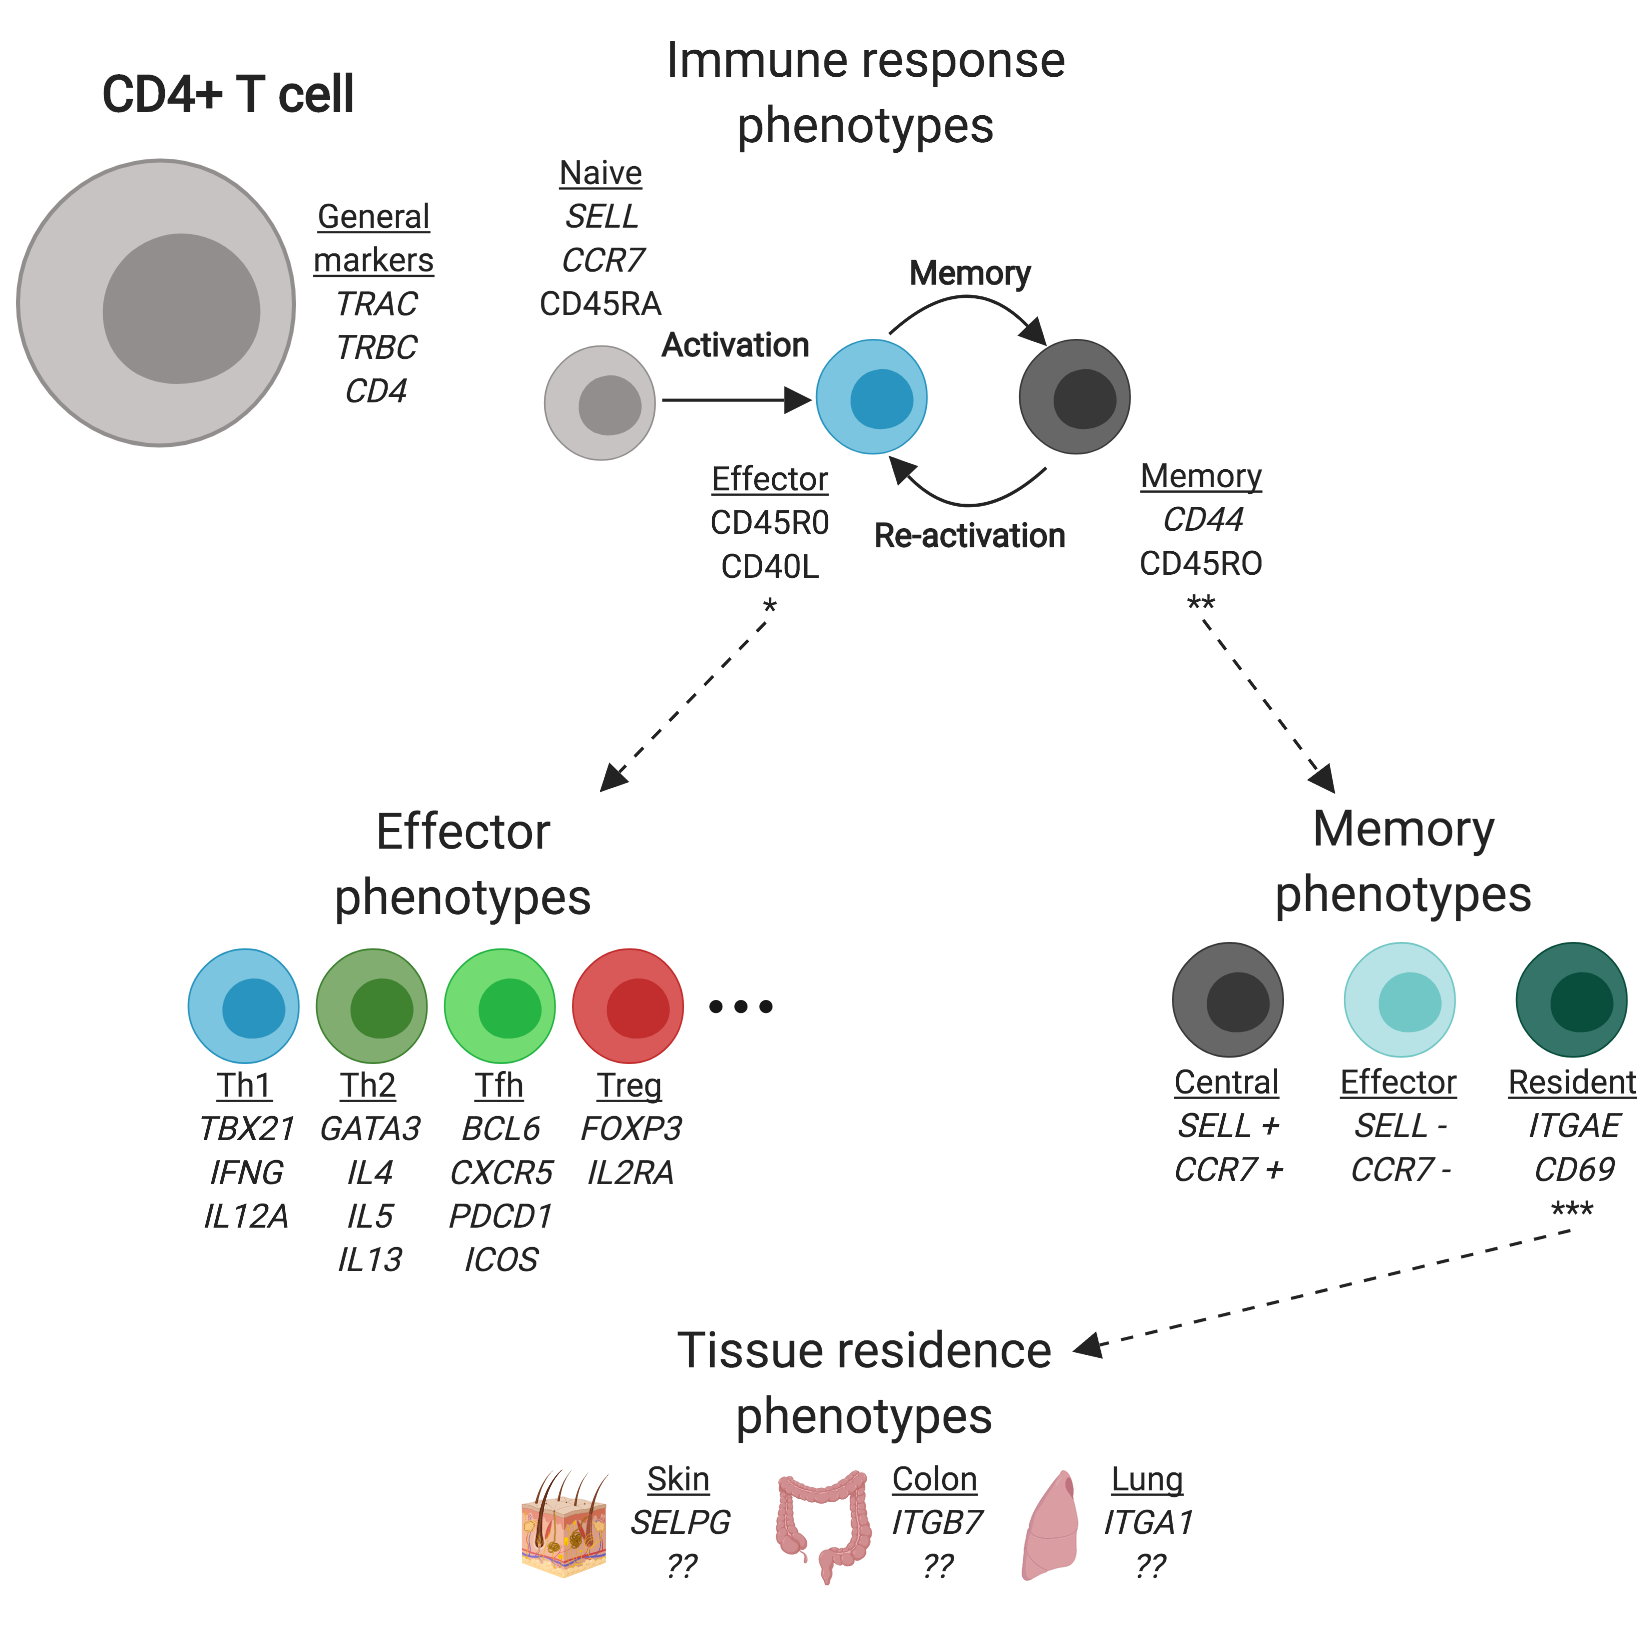
\includegraphics[width=1.0\textwidth]{Chapter1/Figs/chap1_fig1.png} % change word in curlies to change figure
    \caption[T-helper cell heterogeneity and key marker genes]{An overview of known T-helper cell heterogeneity and key marker genes. Beyond their core markers, Th cells can be classified into based on different phenotypes that depend on stage of immune response, the type of effector function, the type of memory cell they form and their tissue of residence (a topic understudied comparatively to the rest).}
    \label{fig:chap1_fig1}
\end{figure}

CD4\textsuperscript{+} T cells are the other side of T cell. Also known as T-helper (Th) cells, these lymphocytes are credited with the organisation of immune response, producing cytokines that serve as triggers or blockers of particular immune reactions~\citep{luckheeram_cd4+t_2012}. Th cells recognise antigens presented by the MHC class II, present only on the membrane of dendritic cells, mononuclear phagocytes, some endothelial cells, thymic epithelial cells (important during T cell selection for functional, non-self-responding TCR), and B cells. This interaction, combined with signalling from the media where the cell is acting, induce an activation programme of the cell that is specific to the external threat being handled. It is not then surprising that CD4\textsuperscript{+} cells encompass a large transcriptional plasticity, which results in diverse related phenotypes (Figure~\ref{fig:chap1_fig1}). Th cells have classically been organised in various effector phenotypes on the grounds of their cytokine output~\citep{mosmann_two_1986,schmitt_regulation_2015}, correlating with the type of immune response at hand. T cells producing different signalling molecules will interact with different cells. These effector phenotypes are not the sole drivers of variability between Th cells, rather they exist in parallel with other expression programmes. Upon finishing responding to an infection, T cells can go into a lowly replicative memory state in which they will save the TCR that drove the specialized response. The various memory states relate to the level of activation of the cell, but also to its tissue of residence. Cells expressing the chemokine receptor CCR7 are in a more naive, non-stimulated state, and also target lymphoid tissues like lymph nodes or the spleen, where most of antigen presenting to CD4\textsuperscript{+} T cells takes place. Other tissue-homing and residency phenotypes exist, all of them characterised by the involvement of one or more chemokine receptors or adhesion molecules like integrins. Nonetheless, tissue-specificity in T-helper cells, and even more broadly in immune cells, is still generally understudied. Yet recent developments using single-cell high throughout methods have tackled this questions~\citep{wong_high-dimensional_2016,scott_transcription_2018}, and it is expected that future efforts will rely on the accumulation of data to extract these patterns from cross-tissue samples.

%% regulation and plasticity of T cell identity (mention Treg functions, mention homeostatic functions)
Among the phenotypic variability of T-helper cells we can find the particular subset termed T-regulatory (Treg) cells. They different from most Th cell subtypes in that, rather than boosting immune response, they are responsible for dampening it~\citep{sakaguchi_immunologic_1995}. This regulatory role in the immune system is of dire importance. Leaving the immune response unchecked can lead to destructive responses that will adversely affect the organism, as is seen in autoimmune diseases. Treg cells were originally identified by their high expression of CD25, but as a subset they are more clearly defined by the expression of the FOXP3 transcription factor~\citep{hori_control_2003}. Despite the focus on CD4\textsuperscript{+} Treg cells here presented, CD8\textsuperscript{+} cells can also have a regulatory phenotype, yet this are understudied compared to its CD4\textsuperscript{+} counterpart~\citep{yu_recent_2018}.

Treg cells have themselves described to have further subsets, either related to the various parallel programmes that Th cells can adopt or their developmental origin. All T cells develop in the bone marrow and mature in the thymus, where their TCR recombines and is tested for responsiveness to foreign antigens and against self-antigens. However, natural Treg cells are derived from an subset of T cells with an intermediate level of response to self-antigens. This subset is further supplemented by induced Treg cells, which originate from other T-helper cells. While both natural and induced T-regulatory cells share a role, their distinct origins extend their TCR repertoire and thus their action scope~\citep{zhang_subsets_2014}. Beyond this, Treg cells are also subject to memory and tissue-trafficking phenotypes like the remaining Th cells~\citep{huehn_developmental_2004}, although these are not as well studied.

Immune cells are also described to have roles beyond defense against pathogens. These roles involve interactions with other non-immune tissues and mostly focus on their maintenance~\citep{gordon_physiological_2017,laurent_immune-mediated_2017}, although the immune system has also been described as relaying signals to the nervous system~\citep{veiga-fernandes_neuro-immune_2016}. Treg cells have been increasingly noted to be relevant, not just for their role in the immune system, but also for their functions beyond it. This regulatory subset has been shown to be involved in tissue repair~\citep{li_regulatory_2018} (chiefly muscle~\citep{burzyn_special_2013}), hair growth~\citep{ali_regulatory_2017}, and homeostatic regulation of gut microbiota~\citep{cebula_thymus-derived_2013} and adipose tissue~\citep{cipolletta_adipose_2014,sharma_emerging_2018}. These functions, being widespread in the organism, consequently rely on and efficient trafficking and tissue localization scheme~\citep{liston_homeostatic_2014}. Despite the clear potential for biomedicine in understanding how these migration and adaptation programmes are constituted and regulated~\citep{agace_tissue-tropic_2006}, work on this front is still in need for more robust comparisons across tissues, that additionally incorporate the population heterogeneity aspect and how they relate between different locations.


\nomenclature[z-TCR]{TCR}{T Cell Receptor}
\nomenclature[z-APC]{APC}{Antigen-Presenting Cell}
\nomenclature[z-MHC]{MHC}{Major Histocompatibility Complex}
\nomenclature[z-Th]{Th}{T-helper (cells)}
\nomenclature[z-Treg]{Treg}{T-regulatory (cells)}

%********************************** % Fifth Section  *************************************
\section{Tissue-specific gene expression}  %Section - 1.5 
\label{section1.5}

%% Advances in tissue biology from RNA-seq
%% RNA-seq used to compare tissue, discover pathways, understand tissue function
%% also mention primary cell work
Histological studies have uncovered many details of organ biology and physiology. Tissue staining is routinely used in pathology, and a better understanding of which molecules are markers of different tissues and cells in steady-state can result in important medical advancements.

Early studies in transcriptomics, that relied on microarrays, took an interest in dissecting transcriptional responses to metabolic shifts~\citep{derisi_exploring_1997} and disease (with a particular focus in cancer)~\citep{rhodes_large-scale_2004}, with homeostatic tissue sample comparison only appearing later~\citep{shyamsundar_dna_2005}. 
RNA-sequencing has, from its inception, been linked to the unraveling of cross-organ and tissue differences~\citep{mortazavi_mapping_2008}. Compared with preceding technologies, RNA-seq was capable of detecting a broader variety of transcripts in an unbiased way, along with high confidence splice junctions and allele-specific expression, with the added benefit of doing it for a lower cost~\citep{wang_rna-seq:_2009}. RNA-seq was quickly adopted and improved (see Section~\ref{section1.2}), extending its sensitivity and breadth of applications. Consortia were developed around the use of sequencing technologies for different biomedical purposes, often with RNA-seq taking a pivotal role~\citep{the_cancer_genome_atlas_research_network_cancer_2013,the_encode_project_consortium_integrated_2012,lonsdale_genotype-tissue_2013}. These large collections of data were instrumental in revealing the functionality of genomic regions as well as the relationships between the tested biological samples. With data from the Genotype-Tissue Expression (GTEx) consortium, it was revealed how human tissues transcriptionally relate to each other, as well as what genes have their expression more dependent on individual or tissue-specific expression~\citep{mele_human_2015}. The Cancer Genome Atlas (TCGA) relied on RNA-seq, as well as other data modalities, from several cancer types to map the similarities between different tumours, and identify potentially important pathways for the treatment of those malignancies~\citep{hoadley_cell--origin_2018}. Comparison between disease samples and steady-state can also be particularly informative, for example in understanding how tumours affect their adjacent tissue~\citep{aran_comprehensive_2017}, or how tumour growth compares to developmental tissues and which pathways are involved~\citep{young_single-cell_2018}. In short, while large databases of expression data can serve as useful resources for broader applications by the scientific community, they can also on their own be mined for important emerging patterns.

%% Cross-species comparative studies
%% RNA-seq used to compare conservation in gene expression
Transcriptomic data can also be analysed beyond one species to gain understanding of the evolutionary links of gene expression programmes. Early microarray analysis showed how human-chimpanzee divergence was especially accentuated when looking at brain RNA~\citep{enard_intra-_2002}. Collection of samples from more species, combined with the use of RNA-seq, augmented the resolution of what gene expression changes could be observed~\citep{brawand_evolution_2011}. Varying divergence rates for different tissues, gene groups and genomic regions, could be observed and associated to different selective pressures and tissue functions. Further studies have since compared other species~\citep{li_comparison_2014} or aspects of the transcriptome~\citep{barbosa-morais_evolutionary_2012}, revealing the intricate way evolution sculpted molecular programmes in different tissues across the tree of life, and what are the core drivers of tissue function. The application of scRNA-seq methods can extend these methods to comparisons between cell types, which results in larger scale comparisons, yet will open a window into how different programmes are specified for cell function in evolution and how they translate across species. It has recently been showed how variability in expression relates to evolution of innate immune response in fibroblasts~\citep{hagai_gene_2018}. Data from this study has been further used to test an artificial intelligence method that was capable of accurately predict species-specific responses solely based on the data from the remaining organisms sampled~\citep{lotfollahi_generative_2018}. As well as understanding evolutionary biology of cell types or immune responses, these types of studies and applications can have considerable impact in translating results from model organisms into the clinic.



%********************************** % Sixth Section  *************************************
\section{Insights and scope of this thesis}  %Section - 1.6
\label{section1.6}

Single-cell RNA-seq has revolutionized the profiling of cell type heterogeneity over the last decade. This has allowed for a deep, unbiased look into several organs and organisms, profiling hundreds of cell types with ground breaking resolution. At the same time, progress was made in computationally combining datasets for further analysis. As an increasing number of scRNA-seq datasets is produced, we come ever closer to a first draft of a transcriptional Human Cell Atlas, showcasing the full spectrum of cellular variety in our species.

The expansion in cell throughput is now permitting the study of smaller, rarer subpopulations. While specific cell types can still be sorted prior to sequencing for deeper profiling, unknown and underrepresented cell types will require larger numbers to be detected. This profound transcriptional portrayal of cells also often results in valuable resources that can be examined for functional targets of novel therapies and assays, which is especially true when studying immune cells. Developing directed cell therapies is a long-term goal of many medical fields, but a thorough knowledge of key cell types is still needed.

A transcriptional reference for cell types can be a key resource for those employing scRNA-seq. Having a ready-to-use resource that draws on the combined knowledge of the data generated would provide immediate assistance for automatic annotation of novel projects. Additionally, an exhaustive and integrated collection can be very informative about cell and tissue biology. However, the limits of this integration should also be tested and examined.

After this introductory chapter, Chapter~\ref{chap:Treg} will show a deep dive into T-regulatory cell heterogeneity using single-cell RNA-seq. Treg cells have been shown to have critical roles in steady-state and disease, but it is still not fully understood which subpopulations fulfill which functions in different tissues, and how this heterogeneity relates to cross-tissue diversity. The chapter will describe Treg cell subpopulations detected in mouse in different tissues and how they compare to other resident T-helper cells. These subpopulations reflect different activation states, and form a phenotypic continuum between peripheral tissues (skin and colon) and their respective draining lymph nodes. The first sections will also discuss the limits of heterogeneity detection using scRNA-seq, especially when using two different protocols. Lastly, a mouse-to-human comparison will be presented, comparing conservation and divergence of gene programmes and Treg cell subpopulations.

Chapters~\ref{chap:CT_method} and~\ref{chap:CT_bio} will focus on the use of broad scRNA-seq data collections to create informative references for automatic cell type annotation. Chapter~\ref{chap:CT_method} will detail the development of a pipeline to integrate diverse scRNA-seq datasets and cluster them into meaningful groups that approximate commonly defined cell identity, and the training of an updatable classifier that can be used to annotate new datasets. All annotation data available from these datasets is also collected, and the classifier train is also in itself informative. Thus, Chapter~\ref{chap:CT_bio} will be centered on the dissection of this data collection and what patterns are learned by the classifier and the pipeline.

This thesis ends in Chapter~\ref{chap:conc}, where I will be discussing the higher picture of the results described in this thesis. This chapter will explore what to what detail cell identity can be deconstructed, and what that means for informative automated annotation of new datasets, as well as to our understanding of cell biology and how they are categorized. 
%!TEX root = ../thesis.tex
%*******************************************************************************
%****************************** Second Chapter *********************************
%*******************************************************************************

\chapter{Tissue adaptation of T-regulatory cells} \label{chap:Treg}

\ifpdf
    \graphicspath{{Chapter2/Figs/Raster/}{Chapter2/Figs/PDF/}{Chapter2/Figs/}}
\else
    \graphicspath{{Chapter2/Figs/Vector/}{Chapter2/Figs/}}
\fi

Non-lymphoid tissues (NLTs) harbour a pool of adaptive immune cells with largely unexplored phenotype and development. We used single-cell RNA-seq to characterise 35000 CD4\textsuperscript{+} regulatory (Treg) and memory (Tmem) T cells in mouse skin and colon, their respective draining lymph nodes (LNs) and spleen. In these tissues, we identified Treg cell subpopulations with distinct degrees of NLT phenotype. Subpopulation pseudotime ordering and gene kinetics were consistent in recruitment to skin and colon, yet the initial NLT-priming in LNs and the final stages of NLT functional adaptation reflected tissue-specific differences. Predicted kinetics were recapitulated using an \textit{in vivo} melanoma-induction model, validating key regulators and receptors. Finally, we profiled human blood and NLT Treg and Tmem cells, and identified cross-mammalian conserved tissue signatures. In summary, we describe the relationship between Treg cell heterogeneity and recruitment to NLTs through the combined use of computational prediction and \textit{in vivo} validation.

This chapter has been published in \textit{Immunity} as \textit{Single-cell transcriptomics of regulatory T cells reveals trajectories of tissue adaptation}~\citep{miragaia_single-cell_2019}, with the exception of Section~\ref{section2.7} and parts of Sections~\ref{section2.8} and~\ref{section2.9}. The Methods section only includes the computational steps. The remaining experimental methods, as well as the supplementary figures, can be found in Appendix~\ref{appendix:treg}.

\textbf{Additional contributions}: experiments in this chapter were performed by Ricardo J Miragaia. The study was designed by Ricardo J Miragaia, Sarah A Teichmann, Agnieszka Chomka, Fiona Powrie, and myself. Ricardo J Miragaia is a leading co-author of the manuscript. Full acknowledgements can be found in Appendix~\ref{appendix:treg}.


\nomenclature[z-Tmem]{Tmem}{T-memory (cells)}
\nomenclature[z-NLT]{NLT}{Non Lymphoid Tissue}
\nomenclature[z-LT]{LT}{Lymphoid Tissues}
\nomenclature[z-LN]{LN}{Lymph Nodes}

\section{Introduction}
\label{section2.1}
T-regulatory (Treg) cells are a specialised CD4\textsuperscript{+} T cell subset which control immune responses and play a central role in homeostasis~\citep{Sakaguchi2004-kz,Izcue2009-sq}. Recent studies have described unique tissue-specific adaptations of non-lymphoid tissue (NLTs) Treg cells distinct from their lymphoid tissue (LT) counterparts. This includes acquisition of an effector phenotype with expression of transcripts encoding effector molecules (\textit{Ctla4}, \textit{Gzmb}, \textit{Klrg1}), chemokines and their receptors (\textit{Ccr4}), and immunosuppressive cytokines (\textit{Il10})~\citep{Panduro2016-fz,Bollrath2013-fa}, in addition to tissue-specific signature genes associated with their role in each environment~\citep{liston_homeostatic_2014}. Nonetheless, their full transcriptional phenotype and its reflection on NLT population heterogeneity is yet to be uncovered.

Trafficking of T cells to NLTs occurs in steady-state conditions and development~\citep{Kimpton1995-ei,Thome2015-vg} as well as in response to harmless stimuli at barrier surfaces such as commensal bacteria and dietary antigens~\citep{Ivanov2008-uz}. Treg cell migration requires tissue-specific cues involving integrins, chemokine and other G-protein coupled receptors~\citep{Cepek1994-sj,Kim2013-pu,Chow2015-tc}.

To provide a deeper insight into Treg cell populations in NLTs, we analysed single-cell RNA-seq (scRNA-seq) data of Treg cells from mouse colon and skin, and compared them to LT populations. We identified various transcriptionally distinct clusters of Treg cells in LTs and NLTs, namely a subpopulation in the LTs which showed heavy priming to the NLT environment. Pseudotime ordering of these subpopulations further revealed the transcriptomic adaptations occurring in Treg cells during their transition from the lymph node to barrier tissues. Our results show that these steady-state adaptations share a core signature between bLN-to-skin and mLN-to-colon trajectories, indicative of a general NLT residency programme in barrier tissues. These findings were recapitulated during \textit{de novo} Treg cell recruitment to melanoma in a murine model system. Lastly, we examined the evolutionarily conservation of NLT Treg cells’ identity between mouse and human.


\section{Treg and Tmem cell identity in NLTs is driven by a common expression module}
\label{section2.2}
We performed scRNA-seq on isolated CD4\textsuperscript{+}Foxp3\textsuperscript{+} (Treg) and CD4\textsuperscript{+}Foxp3\textsuperscript{-}CD44high memory (Tmem) T cells (Figure~\ref{fig:appA_fig1}A) from two barrier NLT sites - the colonic lamina propria (hereinafter referred to as colon) and the skin - their lymphoid counterparts in the draining mesenteric and brachial lymph nodes (mLN and bLN), and the spleen from a Foxp3-GFP mouse reporter line~\citep{Bettelli2006-dw} (Figure~\ref{fig:chap2_fig1}A). We will refer to Treg and Tmem cells together as CD4\textsuperscript{+} T cells. For each sorted population, single-cells were captured using the droplet-based microfluidic system Chromium (10x Genomics), hereinafter referred to as 10x. We obtained 30396 good quality cells (see Methods, Figure~\ref{fig:appA_fig1}C, Table S1). Using the same gating strategy, two Smart-seq2~\citep{picelli_full-length_2014} plate-based datasets were produced independently. These confirmed findings drawn from the 10x, and complemented them with higher gene coverage and full T cell receptor (TCR) sequences.

\begin{figure}[ht!] 
\centering    
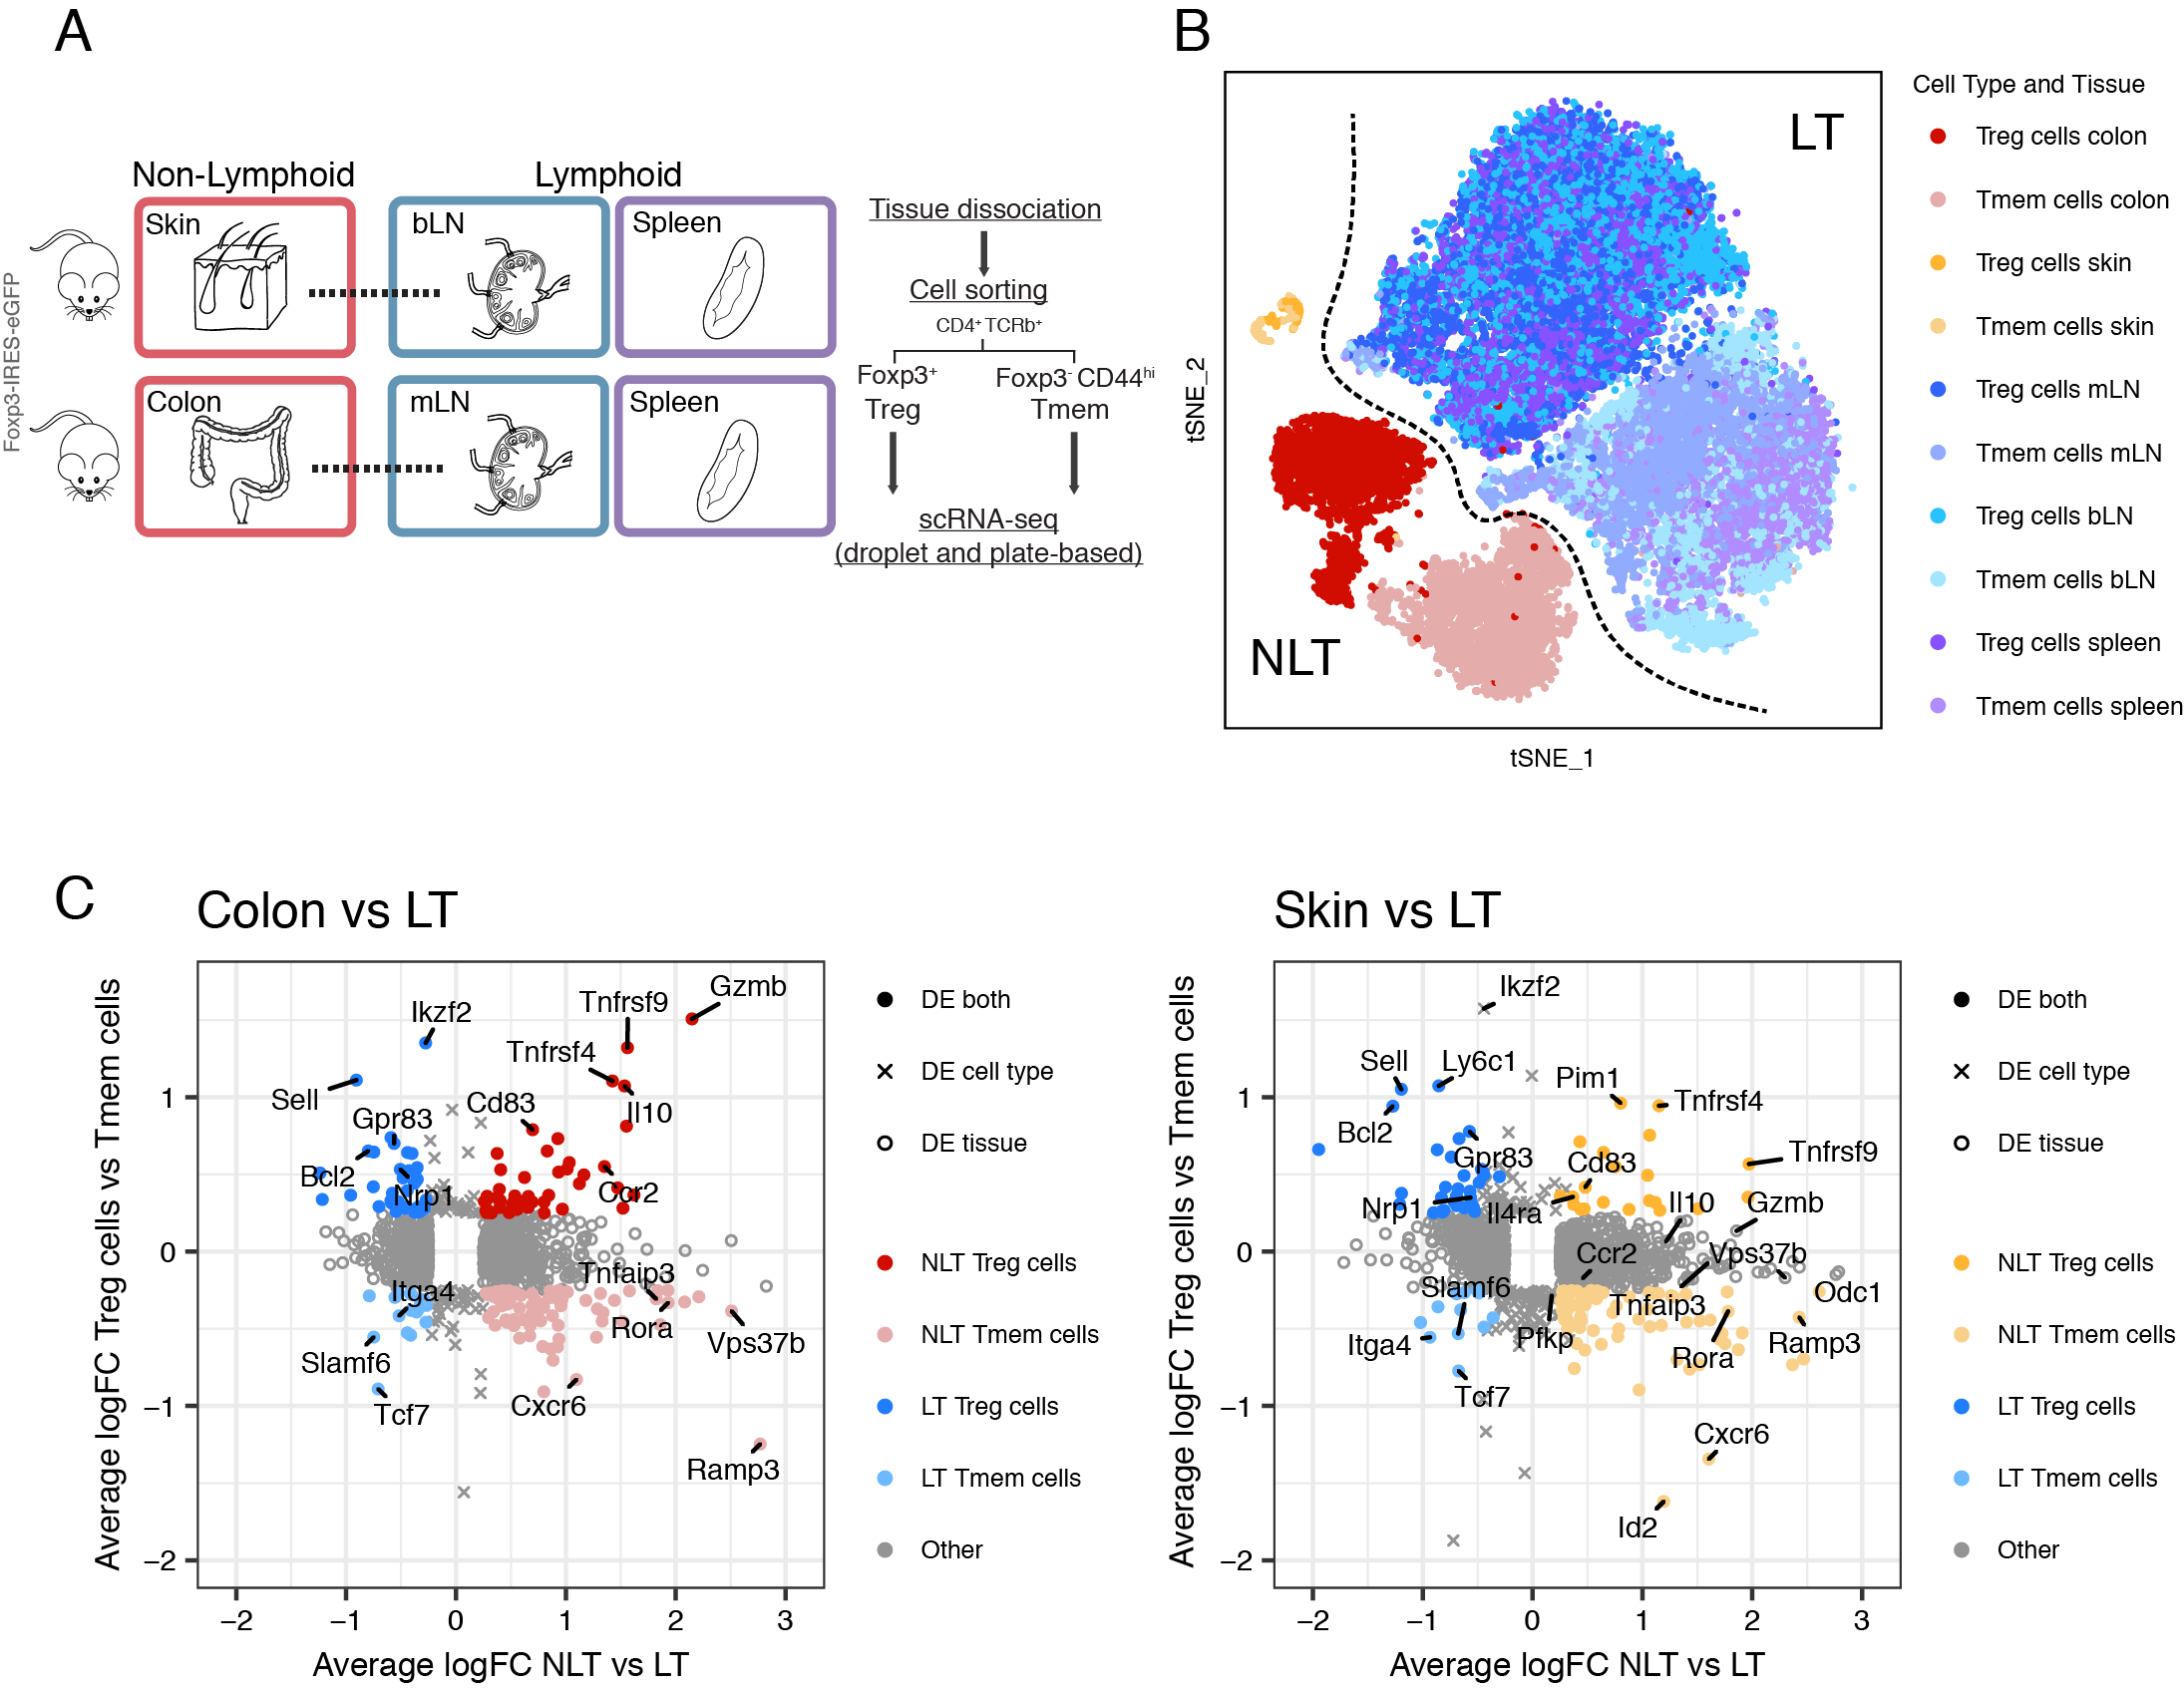
\includegraphics[width=1.0\textwidth]{Chapter2/Figs/chap2_fig1.png} % change word in curlies to change figure
\caption[Steady-state scRNA-seq datasets of CD4\textsuperscript{+} T cells from LT and NLT]{\textbf{Steady-state scRNA-seq datasets of CD4\textsuperscript{+} T cells from LT and NLT}\newline\textbf{(A)} Experimental design for scRNA-seq data collection. \textbf{(B)} t-SNE representing all Treg and Tmem cells that passed quality control. \textbf{(C)} Genes defining the identity of Treg and Tmem cells in lymphoid and non-lymphoid tissues. Colon and skin were individually compared with their corresponding draining lymph node and spleen cells. See also Figure~\ref{fig:appA_fig1}.}
\label{fig:chap2_fig1}
\end{figure}

A tSNE projection (Figure~\ref{fig:chap2_fig1}B) after filtering (Figure~\ref{fig:appA_fig1}B; Table S2) showed a division between LT and NLT, with cells from LTs divided into two clusters, according to cell-type. NLT cells formed one single skin cluster and two clusters separating Treg and Tmem cells from colon (Figure~\ref{fig:chap2_fig1}B). We defined gene expression signatures for Treg and Tmem cells in peripheral tissues by examining differentially expressed (DE) genes between all NLT and LT cells and, in parallel, between Treg and Tmem cells (Figure~\ref{fig:chap2_fig1}C). NLT T cell populations are characterised by the expression of several elements of the TNFRSF-NF-${\upkappa}$B pathway, including transducers (\textit{Traf1}, \textit{Traf4}, \textit{Traf2b}), effectors (\textit{Nfkb1}, \textit{Nfkb2}, \textit{Rel}, \textit{Rela}, \textit{Relb}) and inhibitors (\textit{Nfkbib}, \textit{Nfkbid}, \textit{Nfkbie}). In Tmem cells, these were accompanied by cytokines (\textit{Tnfsf8}, \textit{Tnfsf11}) and various pathway inhibitors, such as \textit{Tnfaip8}. In contrast, NLT Treg cells expressed TNF receptors (\textit{Tnfrsf4}, \textit{Tnfrsf9}, \textit{Tnfrsf18}) and transducers (\textit{Pim1}), underscoring the importance of signalling via the TNFRSF-NF-${\upkappa}$B axis in controlling Treg cells in the peripheral tissues. Several chemokine receptors appeared DE across tissues and cell types. \textit{Ccr4}, \textit{Ccr8} and \textit{Cxcr4} were upregulated in both colon and skin T cells, while \textit{Ccr1} and \textit{Ccr5} were specific to colon and \textit{Ccr6} to skin. \textit{Cxcr6} was more highly expressed in NLT Tmem cells. We also detected other genes involved in NLT identity (\textit{Crem}, \textit{Rgs2}, \textit{Il1r2}, \textit{Icos}, \textit{Hif1a}, \textit{Kdm6b}, \textit{Gata3}), including some specific to Tmem (\textit{Vps37b}, \textit{Id2}, \textit{Ramp3}, \textit{Tnfsf8}) and Treg cells (\textit{Il10}, \textit{Gzmb}, \textit{Ctla4}, \textit{Cd83}, \textit{Socs2}).

Together, the scRNA-seq datasets collected provide a comprehensive overview of Treg and Tmem cells in multiple lymphoid and non-lymphoid tissues, and identify the TNFRSF-NF-${\upkappa}$B pathway as key to their barrier tissue identity.


\section{Heterogeneity within LT and NLT Treg cell populations}
\label{section2.3}
Treg cell phenotypical and functional heterogeneity has been extensively discussed in recent years~\citep{Josefowicz2012-nh,Campbell2011-uc}. Clustering our data within each tissue grouped Treg cells into distinct subpopulations (Figure~\ref{fig:chap2_fig2}A) with clearly defined marker genes (Figure~\ref{fig:chap2_fig2}B; Table S3). Across lymphoid organs, we identified central and effector Treg (cTreg and eTreg) cell subsets~\citep{Cretney2011-zd,Vasanthakumar2015-jw}. cTreg cells express typical LT-associated markers, such as \textit{Tcf7}, \textit{Bcl2}, \textit{Sell}, \textit{S1pr1}, while eTreg cells expressed a subset of NLT-associated genes, like \textit{Tnfrsf9}, \textit{Relb}, \textit{Ikzf2} and \textit{Pdcd1}. We also detected a subpopulation of Treg cells with high expression of \textit{Stat1} and interferon stimulated genes exclusively in the bLN. A fourth, less frequent population in lymphoid tissues (~5-10\%; Figure~\ref{fig:chap2_fig2}C), which we named Treg NLT-like cells, expresses eTreg cell markers as well as genes characteristic of NLT T cells, such as \textit{Itgae}, \textit{Rora}, \textit{Fgl2}, \textit{Klrg1} (Figure~\ref{fig:chap2_fig2}B). We hypothesize that this population is primed to migrate and adapt to NLTs. Indeed, DE genes between NLT-like Treg cells from mLN and bLN revealed that the colon-homing molecules \textit{Ccr9} and \textit{Itga4}, as well as their regulator \textit{Batf} were upregulated specifically in the mLN, while \textit{Cxcr3} and \textit{Itgb1} were present in the bLN (Figure~\ref{fig:chap2_fig2}E). These differences were not observed between other LN subpopulations (data not shown).

\begin{figure}[tp!] 
\centering    
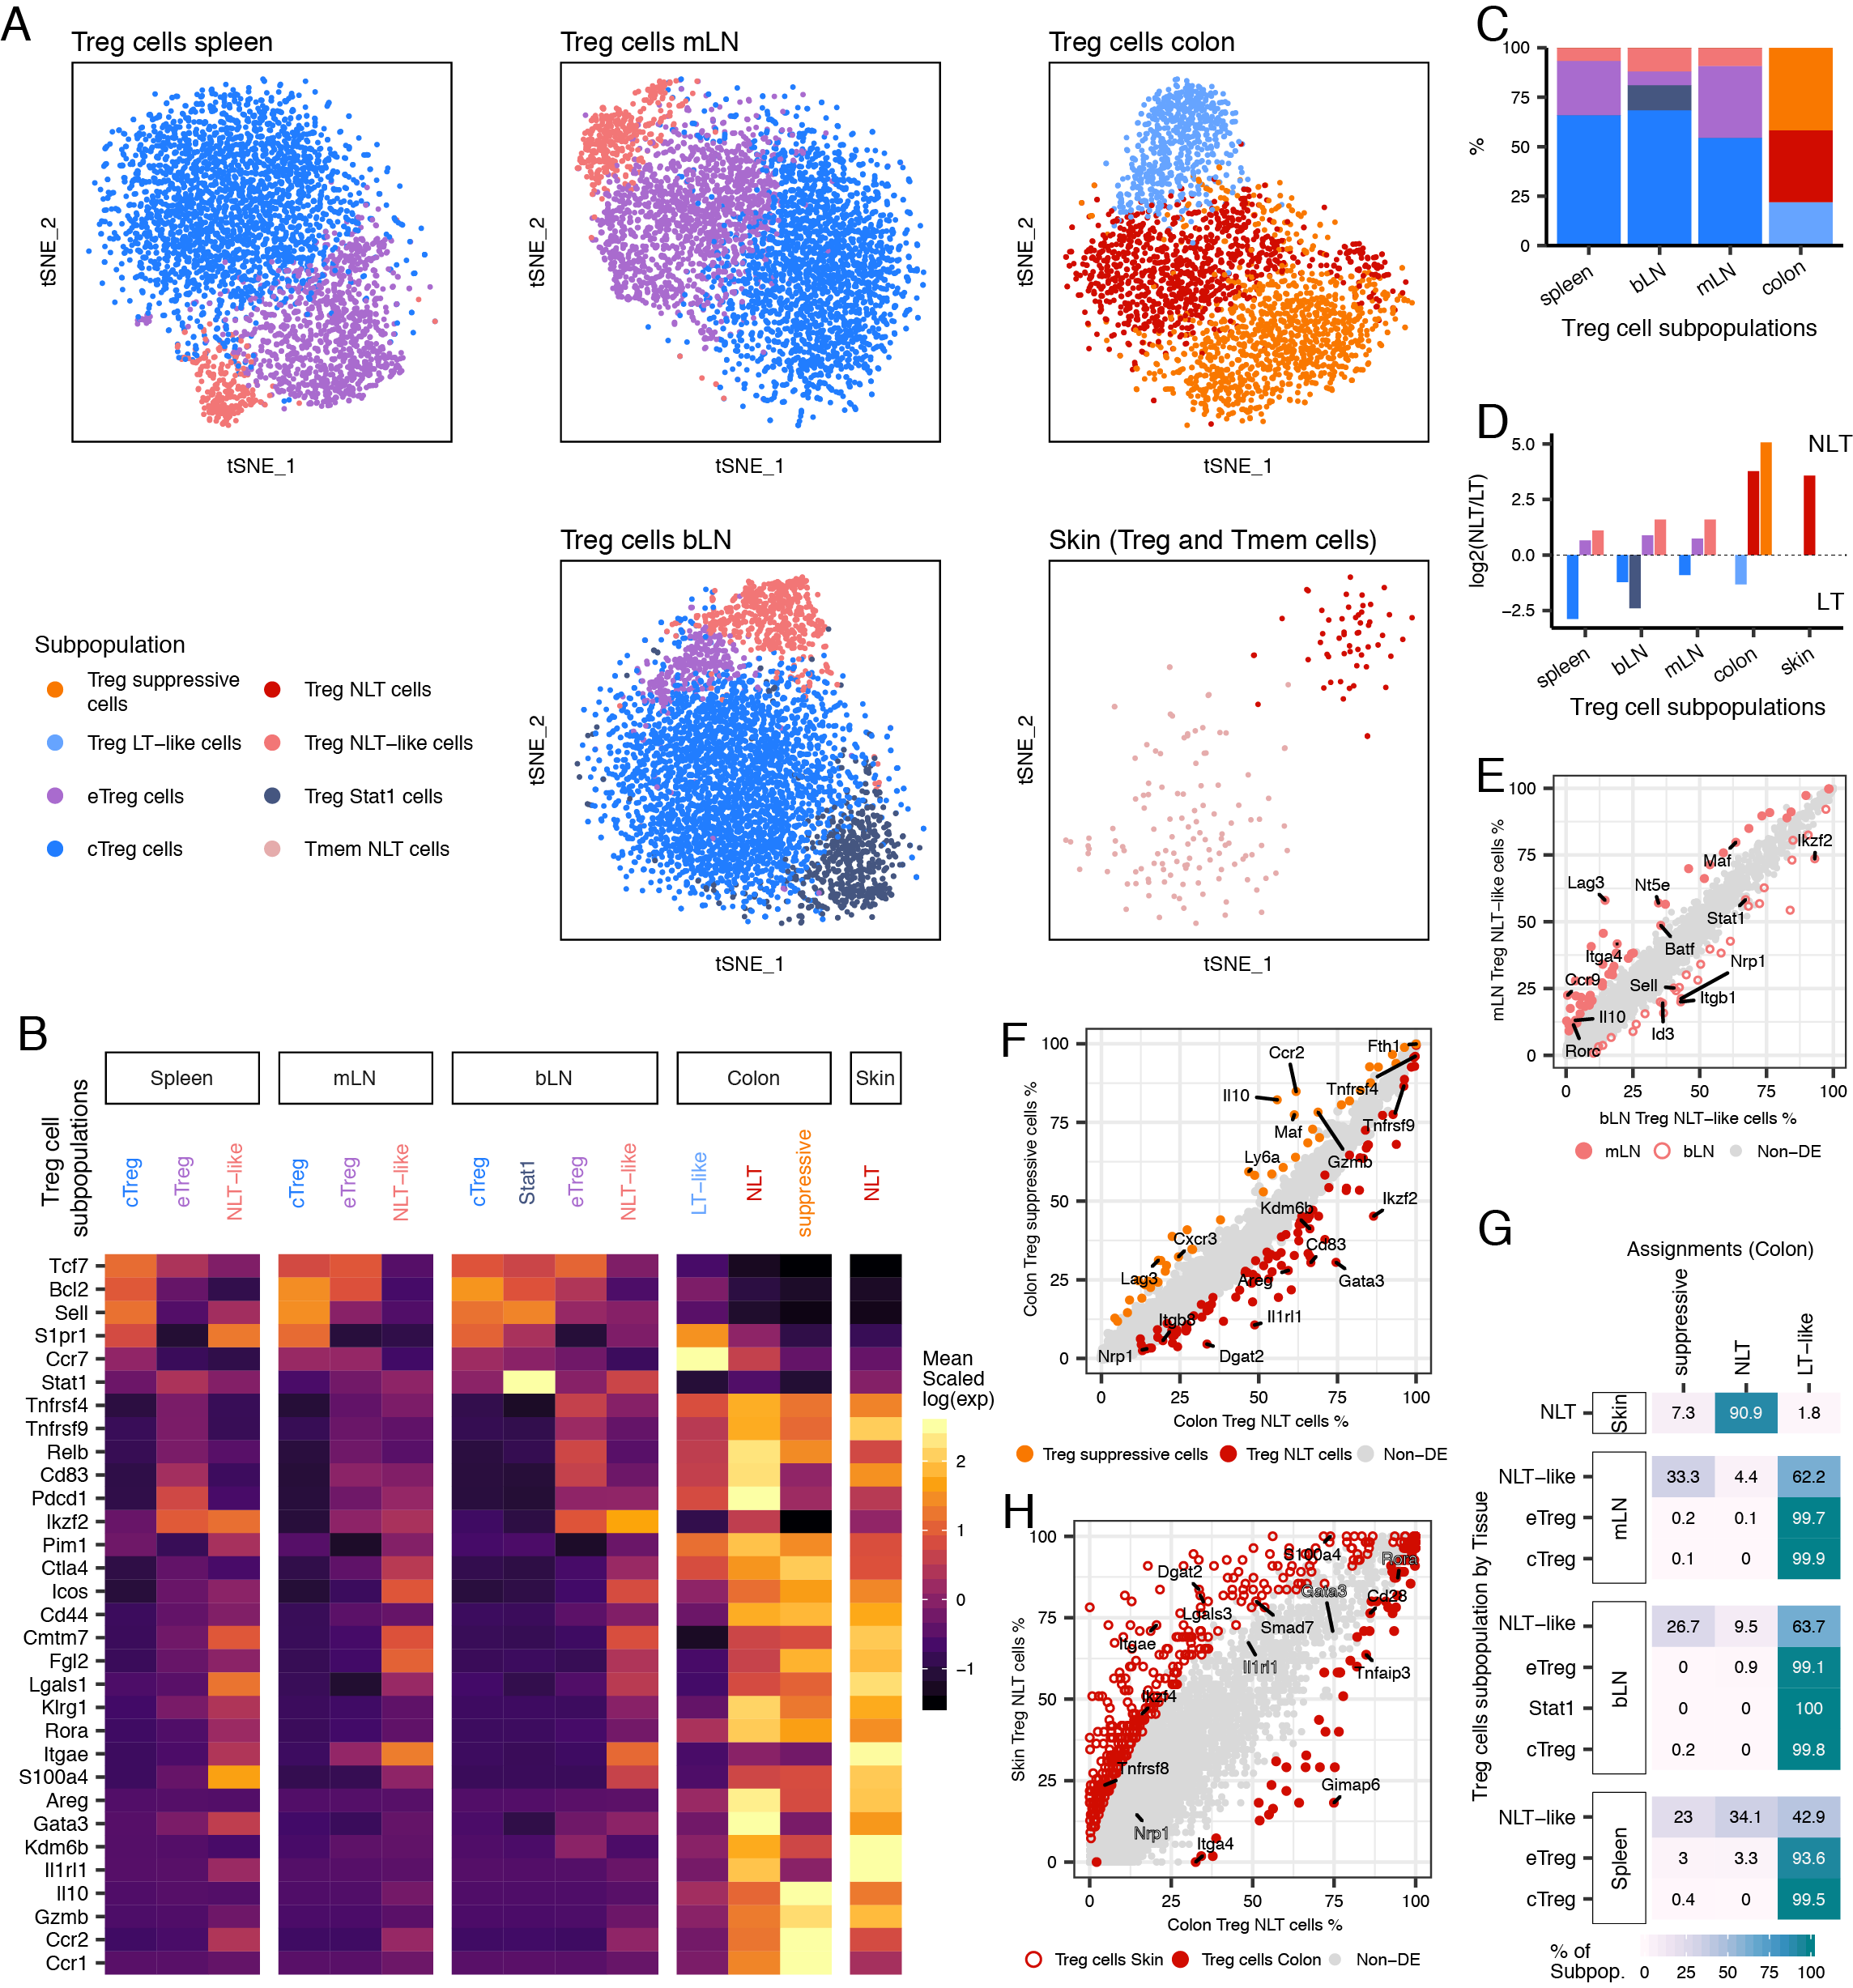
\includegraphics[width=1.0\textwidth]{Chapter2/Figs/chap2_fig2.png} % change word in curlies to change figure
\caption[Heterogeneity within LT and NLT Treg populations]{\textbf{Heterogeneity within LT and NLT Treg populations}\newline\textbf{(A)} t-SNE projections of Treg cells per tissue, coloured by subpopulation. cTreg: central Treg, eTreg: effector Treg. \textbf{(B)} Subpopulation marker gene mean expression (z-score). Values greater than 2.5 or lower than -1.5 are coloured equally. \textbf{(C)} Relative proportions of Treg cell subpopulations within each tissue that revealed heterogeneity. \textbf{(D)} NLT/LT signature score in each Treg cell subpopulation, measured as the ratio between the number of NLT and LT genes that have been identified as significantly upregulated in each cluster. \textbf{(E)} Percentage of cells expressing each gene in Treg NLT-like cells from mLN and bLN. Genes that are upregulated in the bLN subpopulation are represented by an open circle, and genes upregulated in mLN are represented by a filled circle. (Continued on the following page.)}
\label{fig:chap2_fig2}
\end{figure}
\begin{figure}[t]
  \contcaption{(continued) \textbf{(F)} Percentage of cells expressing each gene in colon Treg suppressive and Treg NLT subpopulations. \textbf{(G)} Matching of non-colonic Treg cells to colonic Treg cell subpopulations using a logistic regression model (90${\%}$ accuracy, see Methods). Table shows the percentage of each identified subpopulation (y-axis) that were labelled by the model as each Treg cell cluster (x-axis). \textbf{(H)} Percentage of cells expressing each gene in skin Treg NLT and colon Treg NLT cell subpopulations. See also Figure~\ref{fig:appA_fig2}.}% Continued caption
\end{figure}

To quantify the bias towards LT or NLT phenotypes, we calculated an NLT-LT marker gene signature for each cluster (Figure~\ref{fig:chap2_fig2}D; see Methods). Consistently across all LTs, cTreg cells exhibited a clear LT signature, while eTregs and NLT-like Tregs leaned towards an NLT profile, which was more pronounced in the latter. 

In the colon, we found three subpopulations of Treg cells that we labeled as NLT, suppressive and LT-like. Treg NLT and suppressive cells were present in equal proportions, both exhibiting NLT traits (Figure~\ref{fig:chap2_fig2}C,D). Treg NLT cells in colon express higher amounts of \textit{Gata3}, \textit{Nrp1}, \textit{Areg}, \textit{Il1rl1}, \textit{Ikzf2}, matching the known thymic-derived GATA3\textsuperscript{+}-subpopulation~\citep{Schiering2014-ry,Hu2015-yc}, while suppressive colonic Treg cells expressed more \textit{Il10}, \textit{Gzmb}, \textit{Lag3}, \textit{Cxcr3}, resembling the peripherally-derived ROR${\upgamma}$t\textsuperscript{+}-subpopulation~\citep{Ohnmacht2015-mo,Schiering2014-ry,Sefik2015-jq}. \textit{Rorc} itself, while not present as a marker, appears in a higher percentage of Treg suppressive cells (6.16${\%}$ vs 2.85${\%}$ in colonic Treg NLT cells). Technical limitations for detection of lowly expressed genes by scRNA-seq might account for the difficulty in capturing \textit{Rorc} transcripts. Lastly, LT-like Treg cells differed from other colonic populations by expressing LT-associated genes including \textit{Sell}, \textit{Ccr7}, \textit{Tcf7}, \textit{Bcl2}, and lower amounts of NLT-associated genes such as \textit{Klrg1}, \textit{Cd44}, \textit{Icos}, \textit{Rora}, \textit{Tnfrsf9}, \textit{Itgae} (Figure~\ref{fig:chap2_fig2}B).
In contrast to the colon, and likely as a consequence of fewer cells captured, skin Treg cells did not show evident heterogeneity (Figure~\ref{fig:chap2_fig2}A). They expressed an unequivocal NLT signature (Figure~\ref{fig:chap2_fig2}D), but it was not clear to which colonic Treg cell populations they were most similar (Figure~\ref{fig:chap2_fig2}B). We addressed this by using a logistic regression model to calculate the probability of each skin Treg cell identifying as one of the colonic subpopulations (Figure~\ref{fig:chap2_fig2}G, see Methods). This revealed that most skin Treg cells were more similar to colonic Treg NLT than to Treg suppressive cells. Accordingly, colon Treg NLT cell marker genes \textit{Gata3}, \textit{Il1rl1}, \textit{Tnfrsf4}, \textit{Rora} were not differentially expressed between skin and colon Treg NLT cells (Figure~\ref{fig:chap2_fig2}H, Figure~\ref{fig:appA_fig2}A). Despite their resemblance, differences in function and/or state between skin and colon Treg NLT might reside in a few genes. Among these are \textit{Dgat2}, an enzyme involved in lipid synthesis in skin~\citep{Fagerberg2014-pj}, and \textit{Ikzf4}, a transcription factor relevant for Treg stability~\citep{Sharma2013-ou}.

The same approach applied to Treg cells from the spleen, mLN and bLN (Figure~\ref{fig:chap2_fig2}G) classified most central and effector Treg cells as Treg LT-like cells. Treg NLT-like cells, on the other hand, were more similar to Treg NLT and Treg suppressive cells. Both the mLN and the bLN had a higher proportion of Treg cells assigned as suppressive than spleen, which contained the highest fraction of Treg NLT cells. We confirmed the presence and proportions of Treg cell subpopulations in the Smart-seq2 datasets by matching these cells to the subpopulations found across LTs and NLTs in the 10x dataset (Figure~\ref{fig:appA_fig2}B).

Clustering of Tmem cells revealed multiple subpopulations (T helper-1 (Th1 cell), Th2 cells, Th17 cells, T follicular helper (Tfh) cells, lymphoid) (Figure~\ref{fig:appA_fig2}C and D; Table S3) distributed differently across the tissues analysed (Figure~\ref{fig:appA_fig2}D). Th1, Th2 and Th17 cells in lymphoid tissues exhibited a stronger NLT phenotype than Tmem lymphoid cells and Tfh cells (Figure~\ref{fig:appA_fig2}E), which is likely an indication of their ability to adapt to and function in the NLTs.

In summary, scRNA-seq allowed us to dissect the heterogeneity of Treg cells from LTs and NLTs. We identified NLT- and LT-like Treg cell subpopulations that suggest progressive cross-tissue adaptation to the NLT environment. We found a close correspondence between skin and colonic Treg NLT cells, whilst revealing differences in gene expression that might explain their adaptation to the two environments.


\section{Treg cells adapting to skin and colon share a transcriptional trajectory}
\label{section2.4}
The mechanisms underlying Treg cell recruitment and adaptation from LT to NLT are far from understood. Having identified multiple subpopulations at different stages of NLT adaptation (Figure~\ref{fig:chap2_fig2}D), we further dissected the dynamics of this transition. We obtained evidence of CD4\textsuperscript{+} T cell recruitment from LT to NLT by reconstructing TCR clonotypes using TraCeR~\citep{stubbington_t_2016} from the Smart-seq2 datasets. This showed Tmem and Treg cell clones present in LNs and respective NLTs (Figure~\ref{fig:appA_fig4}A and~\ref{fig:appA_fig4}B), suggesting cell migration between them.

To identify Treg cell LN-to-NLT adaptation trends in the data, we reconstructed a pseudospace relationship between cells by obtaining latent variables (LV) from Bayesian Gaussian Process Latent Variable Modelling (BGPLVM, see Methods)~\citep{Michalis_K_Titsias2010-na}. Along the mLN to colon trajectory laid out by LV0, Treg cells are ordered from cTreg to eTreg cells, followed by NLT-like and LT-like Treg cells, and ending with the overlapping Treg suppressive and Treg NLT cell subpopulations (Figure~\ref{fig:chap2_fig3}A, “Colon” density plot, Figure~\ref{fig:appA_fig3}A). This order matches the increasing expression of NLT marker genes and decrease of LT ones across mLN subpopulations (Figure~\ref{fig:chap2_fig2}B and D). Importantly, Treg NLT-like cells from the mLN partially mixed with Treg LT-like cells from the colon, supporting the notion that NLT adaptation is a continuous process spanning LT and NLT. Overall, LV0 accurately represented the progressive migration and adaptation of Treg cells to the NLT environment, providing a reference to study the gene expression dynamics along this process. Skin and bLN Treg cells were projected onto the latent space defined for colon and mLN, resulting in a similar subpopulation distribution (Figure~\ref{fig:chap2_fig3}A, “Skin” density plot; see Methods). Nevertheless, a similar projection was observed when using just those cells (Figure~\ref{fig:appA_fig3}A and B). Applying the same approach to the Smart-seq2 datasets yielded similar distributions of the inferred cell subpopulations (Figure~\ref{fig:appA_fig2}B) along the LT-to-NLT adaptation trajectory, as well as considerable overlaps between LV correlated genes (Figure~\ref{fig:appA_fig3}C-E). The use of velocyto~\citep{manno_rna_2018} to infer the directionality of adaptation suggests that most Treg cells found in the NLTs, as well as some of the NLT-like Treg and eTreg cells, are adapting towards a more pronounced NLT phenotype (Figure~\ref{fig:appA_fig3}C).

\begin{figure}[pt] 
\centering    
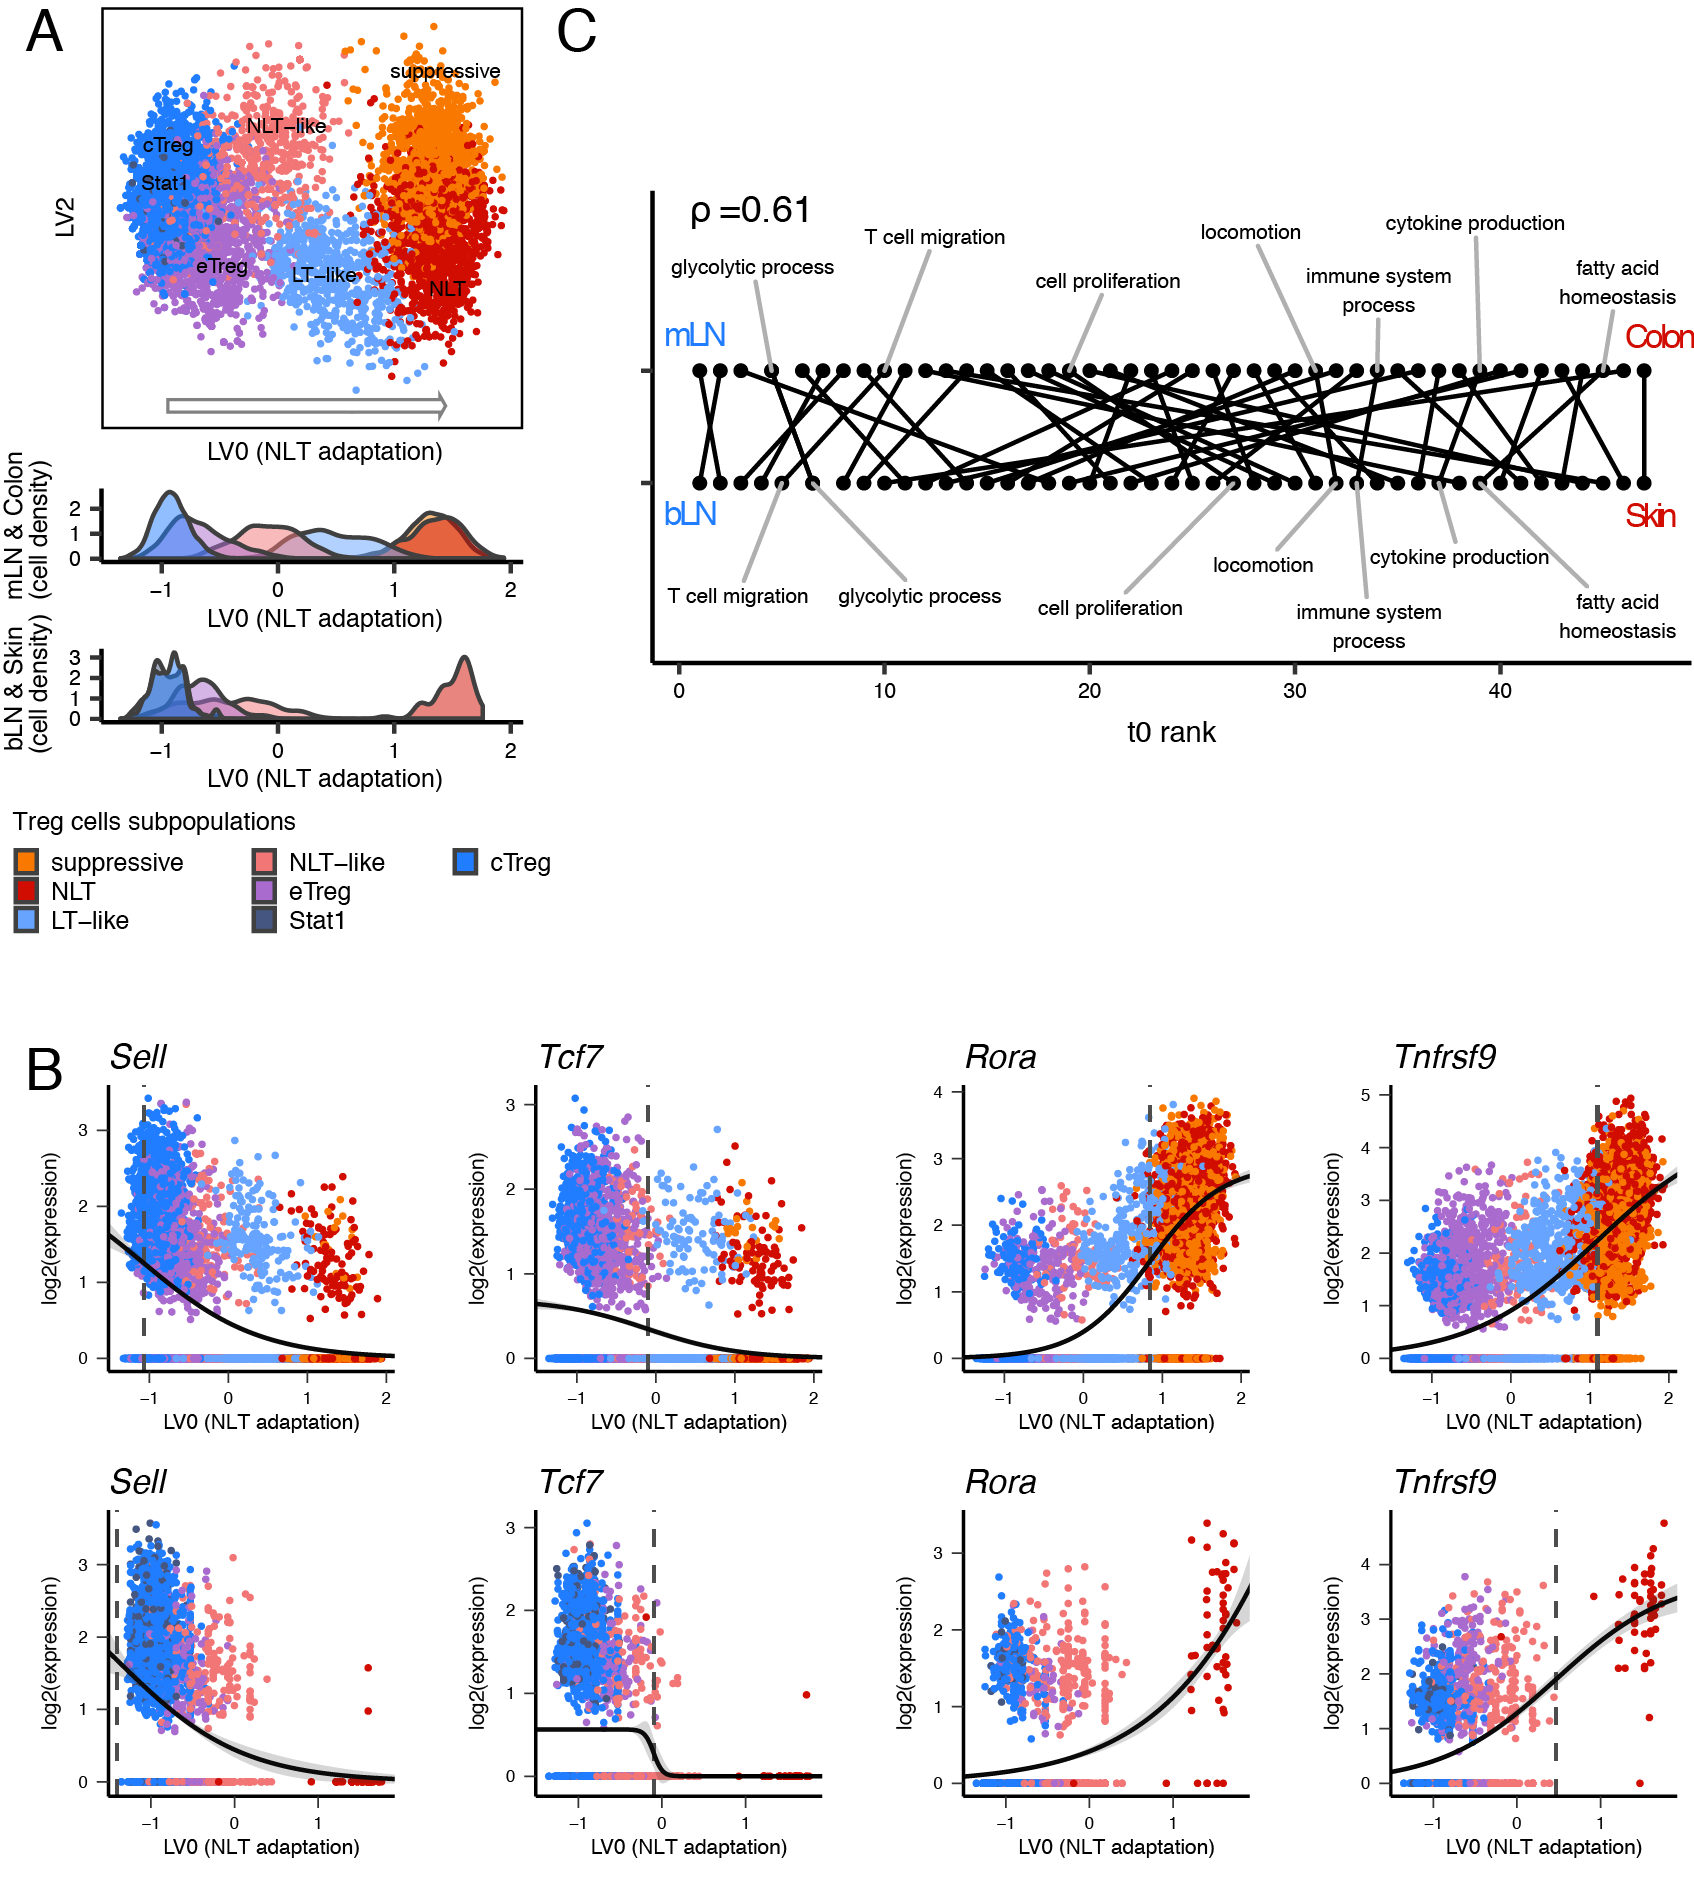
\includegraphics[width=1.0\textwidth]{Chapter2/Figs/chap2_fig3.png} % change word in curlies to change figure
\caption[Reconstruction of Treg cell recruitment from lymphoid to non-lymphoid tissues in steady-state]{\textbf{Reconstruction of Treg cell recruitment from lymphoid to non-lymphoid tissues in steady-state}\newline\textbf{(A)} Top two latent variables (LV) found with BGPLVM for mLN and colonic Treg cells, with bLN and skin Treg cells mapped over the same coordinates. \textbf{(B)} Gene expression in mLN and colon (top) or bLN and skin (bottom) over LV0 modelled as a sigmoidal curve. Dashed vertical line marks the activation point of each gene. \textbf{(C)} Sequence of activation of GO biological processes across the transition to colon (top) or skin (bottom), evidencing a conservation between both trajectories (Spearman’s rho - 0.61). See also Figures~\ref{fig:appA_fig3} and ~\ref{fig:appA_fig4}.}
\label{fig:chap2_fig3}
\end{figure}

We then used the inferred LN-NLT trajectory to identify the cascade of transcriptional changes driving adaptation to NLTs by modelling genes with a sigmoid curve and find their activation or deactivation “times” (Figure~\ref{fig:chap2_fig3}B; Table S4; see Methods). We found 812 and 1209 genes with a switch in expression (either up or down) along the bLN-to-skin and mLN-to-colon trajectories, respectively, with 511 of those being shared. LT-related genes (\textit{Lef1}, \textit{Tcf7}, \textit{Sell}) were downregulated, while NLT associated genes like \textit{Nfil3}, \textit{Ccr8}, \textit{Cxcr6}, \textit{Gzmb} were upregulated. TNFRSF-NF-${\upkappa}$B-related genes (\textit{Tnfrsf1b}, \textit{Tnfrsf4}, \textit{Tnfrsf18}) and the \textit{Batf} transcription factor were upregulated still in the LN, reflecting the relevance of this pathway for eTreg cell development and the NLT phenotype~\citep{Vasanthakumar2017-ib,Vasanthakumar2015-jw}. Towards the NLT side of the trajectory there is evidence of further Treg cell differentiation, with upregulation of additional genes involved in this pathway (\textit{Nfkb2}, \textit{Tnfrsf9}), as well as other effector molecules (\textit{Il10}, \textit{Cd44}). Important regulators for the final tissue adaptation include \textit{Rora}, recently described in skin Treg cells~\citep{Malhotra2018-nz}. We searched for enriched Biological Processes GO Terms, and calculated the mean time of activation or deactivation (t0) of the genes within each term. We found the gene expression kinetics along the adaptation trajectories to skin and to colon to be consistent (Spearman’s rho=0.61, Figure~\ref{fig:chap2_fig3}C): T cell migration and glycolytic process are among the earlier events in both colon and skin, followed by cell proliferation; cytokine production and fatty acid homeostasis emerge towards the end of the adaptation trajectory.

In summary, we determined a continuous trajectory aligning Treg cell subpopulations from bLN, mLN, skin and colon according to the stage of recruitment and adaptation to the NLT environments. Furthermore, the consistent ordering of gene expression programmes shows that gene kinetics leading to NLT adaptation follows a similar regulatory sequence in both bLN-to-skin and mLN-to-colon trajectories.


\section{Treg cell recruitment into skin and melanoma uses common mechanisms}
\label{section2.5}
To validate our findings in steady-state cells, we used a mouse melanoma model to investigate if Treg cell migration and adaptation trajectory to peripheral tissues could be recapitulated. Previous studies analysing human TCR repertoires~\citep{Sherwood2013-jf,Plitas2016-rg} have shown that tumour-Treg cells are likely to be recruited \textit{de novo} from LTs and not from the adjacent NLT, despite exhibiting a phenotype similar to that of NLT Treg cells~\citep{Plitas2016-rg,De_Simone2016-yo}. We therefore purified Treg and Tmem cells from B16.F10 melanomas or PBS controls 11 days after subcutaneous implantation into Foxp3-IRES-eGFP reporter mice~\citep{Haribhai2007-tk} to produce a plate-based scRNA-seq dataset (Figure~\ref{fig:chap2_fig4}A; see Methods).

\begin{figure}[pt] 
\centering    
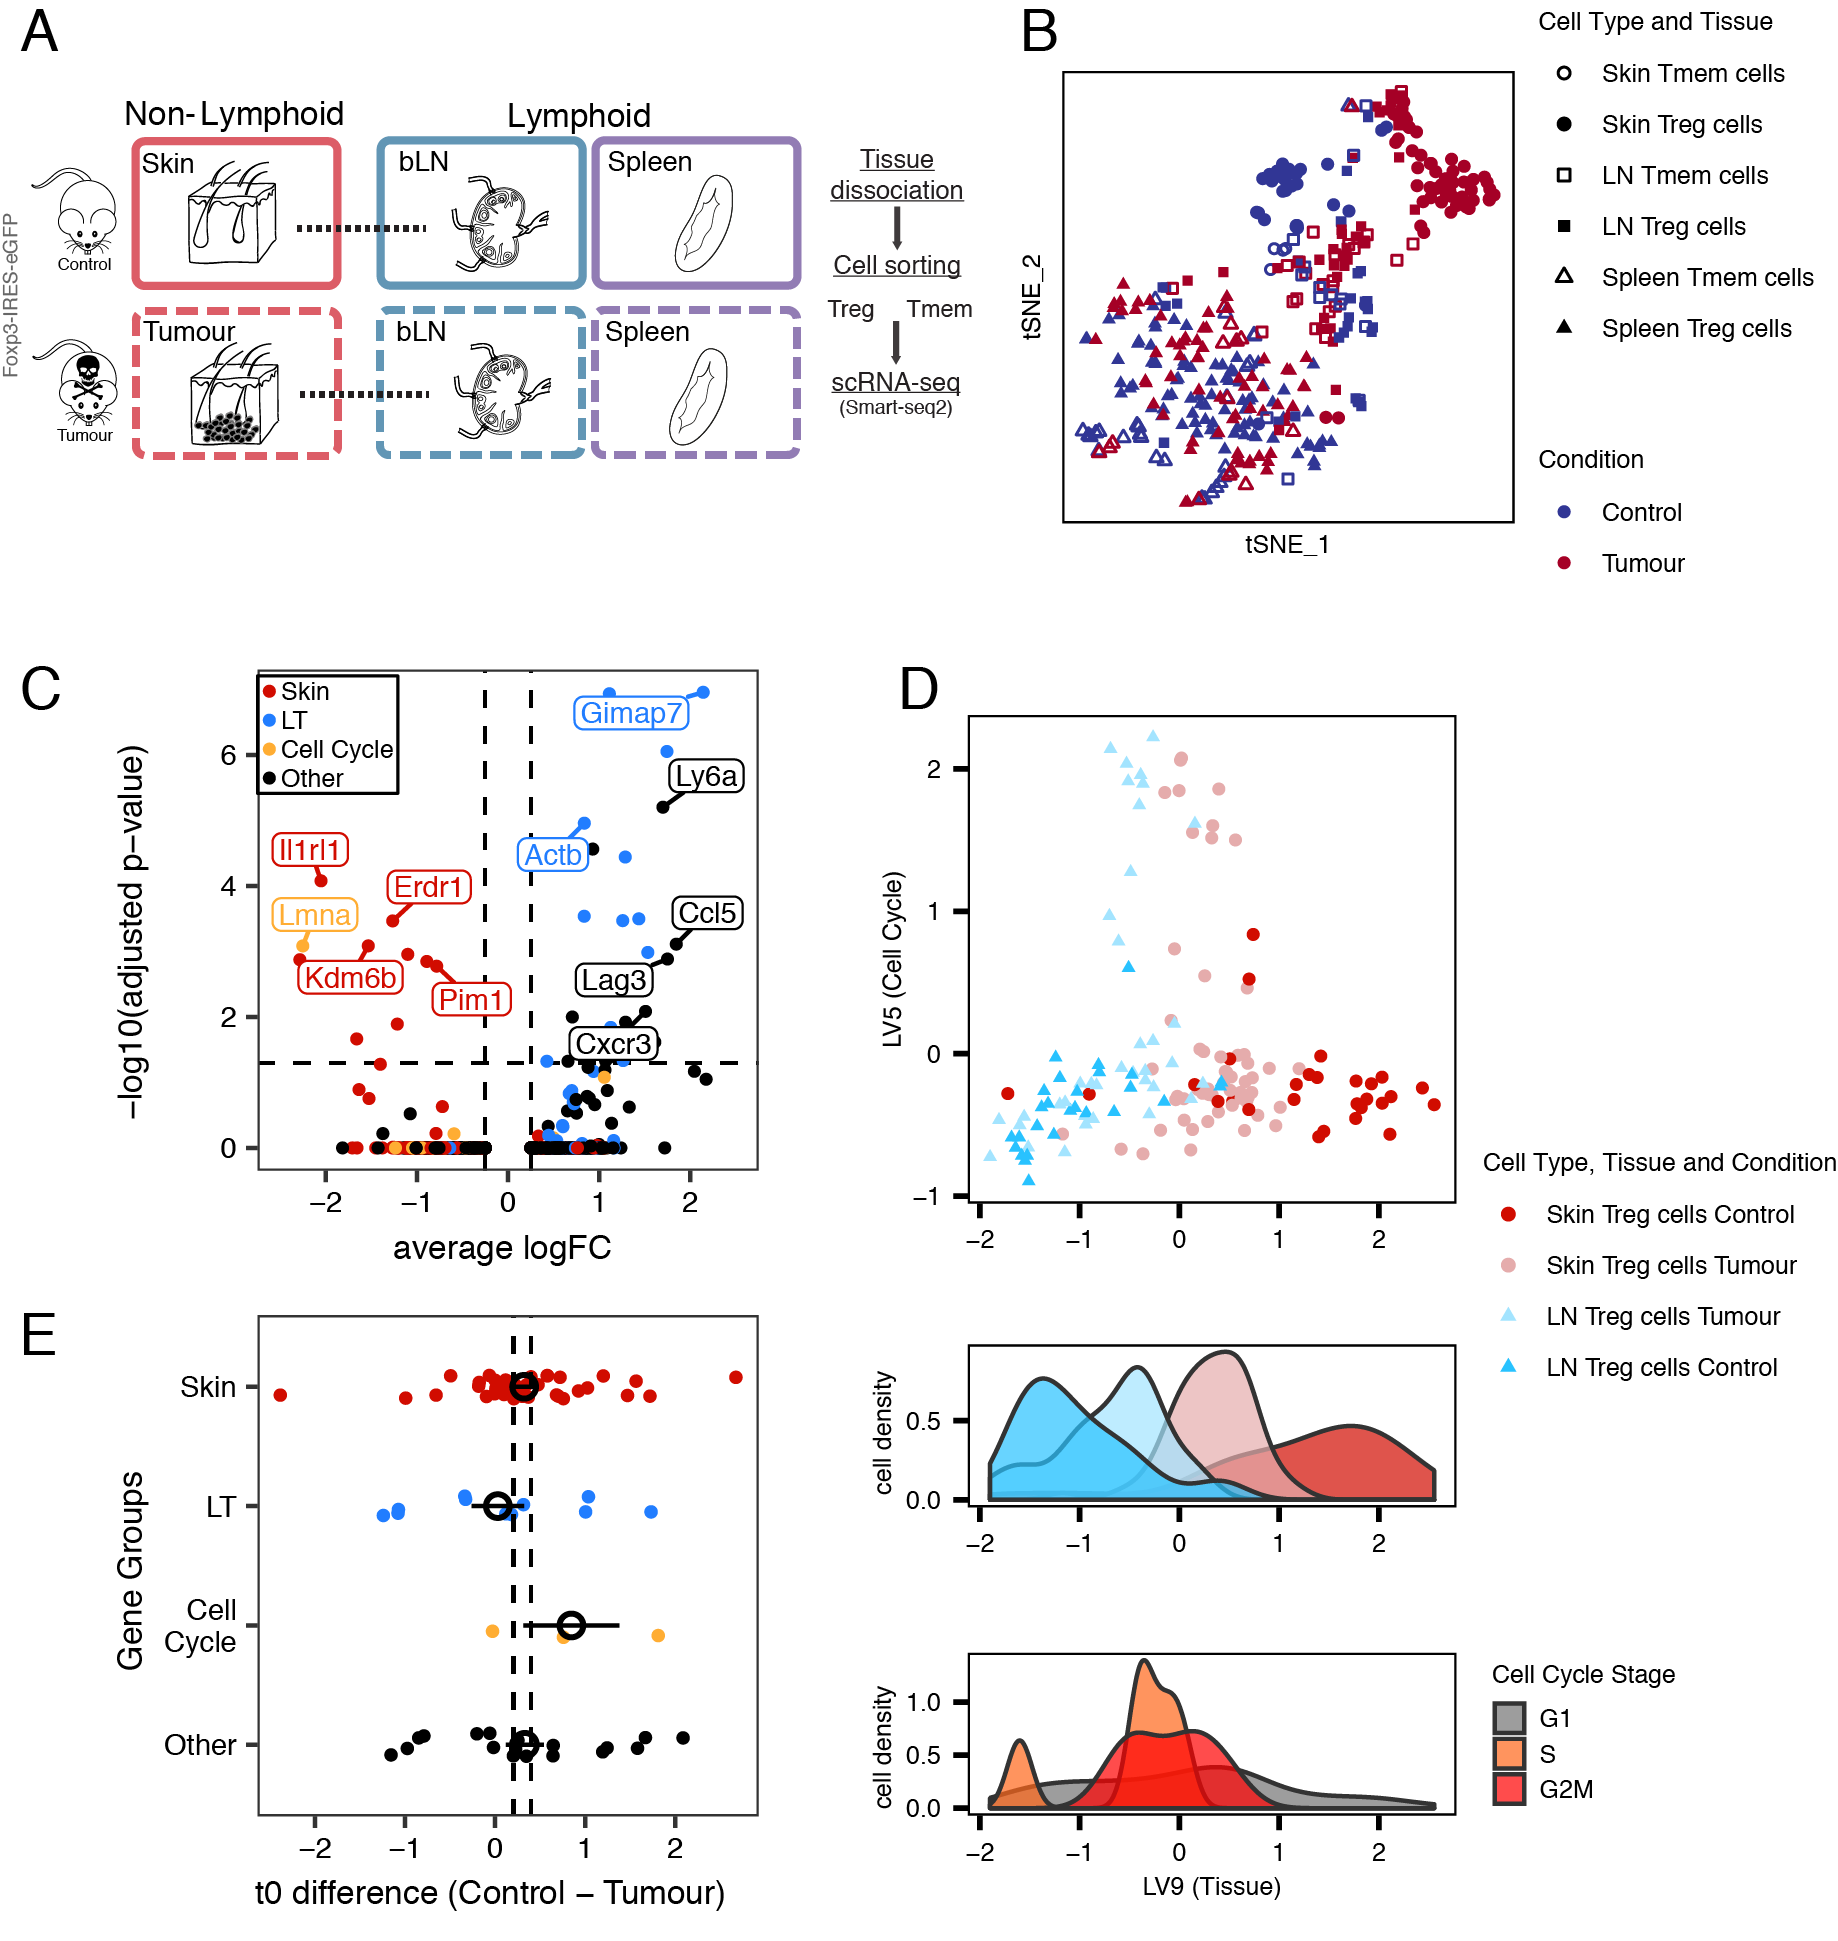
\includegraphics[width=1.0\textwidth]{Chapter2/Figs/chap2_fig4.png} % change word in curlies to change figure
\caption[Recruitment and adaptation of Treg cells to the tumour environment recapitulates steady-state migration]{\textbf{Recruitment and adaptation of Treg cells to the tumour environment recapitulates steady-state migration}\newline\textbf{(A)} Melanoma induction strategy and sampled tissues. \textbf{(B)} t-SNE depicting Treg and Tmem cells from tumour and steady-state skin, draining brachial lymph nodes and spleen. \textbf{(C)} Differential expression between skin and tumour Treg cells. Treg cells classified as cycling were excluded. \textbf{(D)} (top) Latent variables found with MRD-BGPLVM representing cell cycle (LV5) and non-lymphoid tissue recruitment/adaptation of Treg cells (LV9). (bottom) Distribution of cells based on Tissue and Condition and Cell Cycle phase along the recruitment trajectory. (Continued on the following page.)}
\label{fig:chap2_fig4}
\end{figure}
\begin{figure}[t]
  \contcaption{(continued) \textbf{(E)} Difference in activation time (t0) of genes in control and tumour. Genes are classified as being markers of skin, lymph node, cell cycle or other. Coloured points show mean +/- mean standard error for each group. Vertical dashed lines represent the mean +/- standard error for all t0 values. T-test between control and melanoma t0 indicates no change (p-value = 0.2631), with t0 values having a Spearman correlation coefficient of 0.65 between both conditions. See also Figure~\ref{fig:appA_fig5}.}% Continued caption
\end{figure}

Skin and tumour Treg cells clustered separately (Figure~\ref{fig:chap2_fig4}B). As with steady-state skin, we observed shared clonotypes between tumour and bLN Treg cells (Figure~\ref{fig:appA_fig5}B). In the tumour-bearing mice, we detected an additional cluster of cycling cells in both the LN and tumour (Figure~\ref{fig:appA_fig5}A). These observations suggest \textit{de novo} recruitment from LN and simultaneous expansion in both tumour and draining-LN. DE between non-cycling tumour Treg and control skin Treg cells revealed a relatively small number of genes significantly different between the two Treg cell populations (28 upregulated in tumour and 10 in steady-state skin (Figure~\ref{fig:chap2_fig4}C)), in line with recently published human data~\citep{Plitas2016-rg}. Tumour Treg cells upregulate the exhaustion marker \textit{Lag3}~\citep{Malik2017-pw}, as well as \textit{Cxcr3} and \textit{Ccl5}, while control skin Treg cells upregulate skin Treg cell markers such as \textit{Il1rl1}, \textit{Pim1}, \textit{Sdc4}, \textit{Kdm6b} and \textit{Erdr1}. However, skin Treg cell signature genes such as \textit{Batf}, \textit{Tnfrsf4}, \textit{Tnfrsf9}, \textit{Samsn1}, \textit{Tigit}, \textit{Tchp}, \textit{Ccr8}, \textit{Ccr2} and \textit{Itgav} are similarly expressed in both populations.

Next, we sought to obtain a shared migration trajectory of steady-state versus perturbed system (tumour model) Treg NLT cells recruitment. To this end, we used the MRD-BGPLVM algorithm~\citep{Andreas_Damianou_Carl_Ek_Michalis_Titsias_Neil_Lawrence2012-do} (see Methods) to explore gene expression trends across Treg cells from the control skin, tumour and respective draining-LNs together. Two main latent variables were identified, one explained almost entirely by cell-cycle-associated variability (LV5), and one mainly associated with the LT-NLT signature (LV9) (Figure~\ref{fig:chap2_fig4}D, Figure~\ref{fig:appA_fig5}C). Notably, NLT adaptation trajectory (LV9) was strongly related to the trajectories found in control and melanoma conditions when MRD-BGPLVM is applied to each one individually (respectively, 86${\%}$ and 61${\%}$ of genes correlated with LV9 are also correlated with control LV1 and tumour LV1; Figure~\ref{fig:appA_fig5}E-H, see Methods).

Gene kinetics along NLT adaptation (LV9) for each condition show 158 shared genes, with 71${\%}$ of which also present in the steady-state skin trajectory determined previously. Values of t0 remain largely unchanged between control and melanoma (Figure~\ref{fig:chap2_fig4}E), suggesting that NLT recruitment and adaptation follow the same program in homeostatic and perturbed conditions. The tissue adaptation genes shared between control and melanoma include many of the players in the TNFRSF-NF-${\upkappa}$B pathway we previously described in the steady-state (\textit{Tnfrsf9}, \textit{Tnfrsf18}). These were accompanied by genes associated with cell migration and adhesion (\textit{Ccr2}, \textit{Gpr55}, \textit{Plxna2}), transcription factors (\textit{Rora}, \textit{Ikzf3}, \textit{Id2}, \textit{Batf}, \textit{Hif1a}, \textit{Prdm1}), secreted factors (\textit{Lgasl1}), and others related to immune activation and effector states (\textit{Klrg1}, \textit{Icos}, \textit{Tigit}, \textit{Gzmb}).

Despite the similarities between melanoma and control trajectories, cells from both conditions do not completely overlap, and Treg cells could be ordered by NLT adaptation between populations (from least to most adapted cells: control LN, melanoma LN, tumour, and control skin) (Figure~\ref{fig:chap2_fig4}D). This implies that in response to an immune challenge in a barrier tissue, a higher fraction of Treg cells in the LNs acquires NLT adaptations. In fact, for several NLT markers we observed more cells expressing them in the tumour-draining LN compared to the control, e.g. \textit{Id2} (59${\%}$ vs 26${\%}$), \textit{Batf} (57${\%}$ vs 26${\%}$), \textit{Lgals1} (89${\%}$ vs 67${\%}$), further supporting our hypothesis that there is priming of Treg cells to NLTs while still in the LN. Overall, Treg cells from challenged mice recapitulate the steady-state NLT adaptation.


\nomenclature[z-PBS]{PBS}{Phosphate Buffer Saline}

\section{Conserved NLT identity in mouse and human}
\label{section2.6}

\begin{figure}[pt] 
\centering    
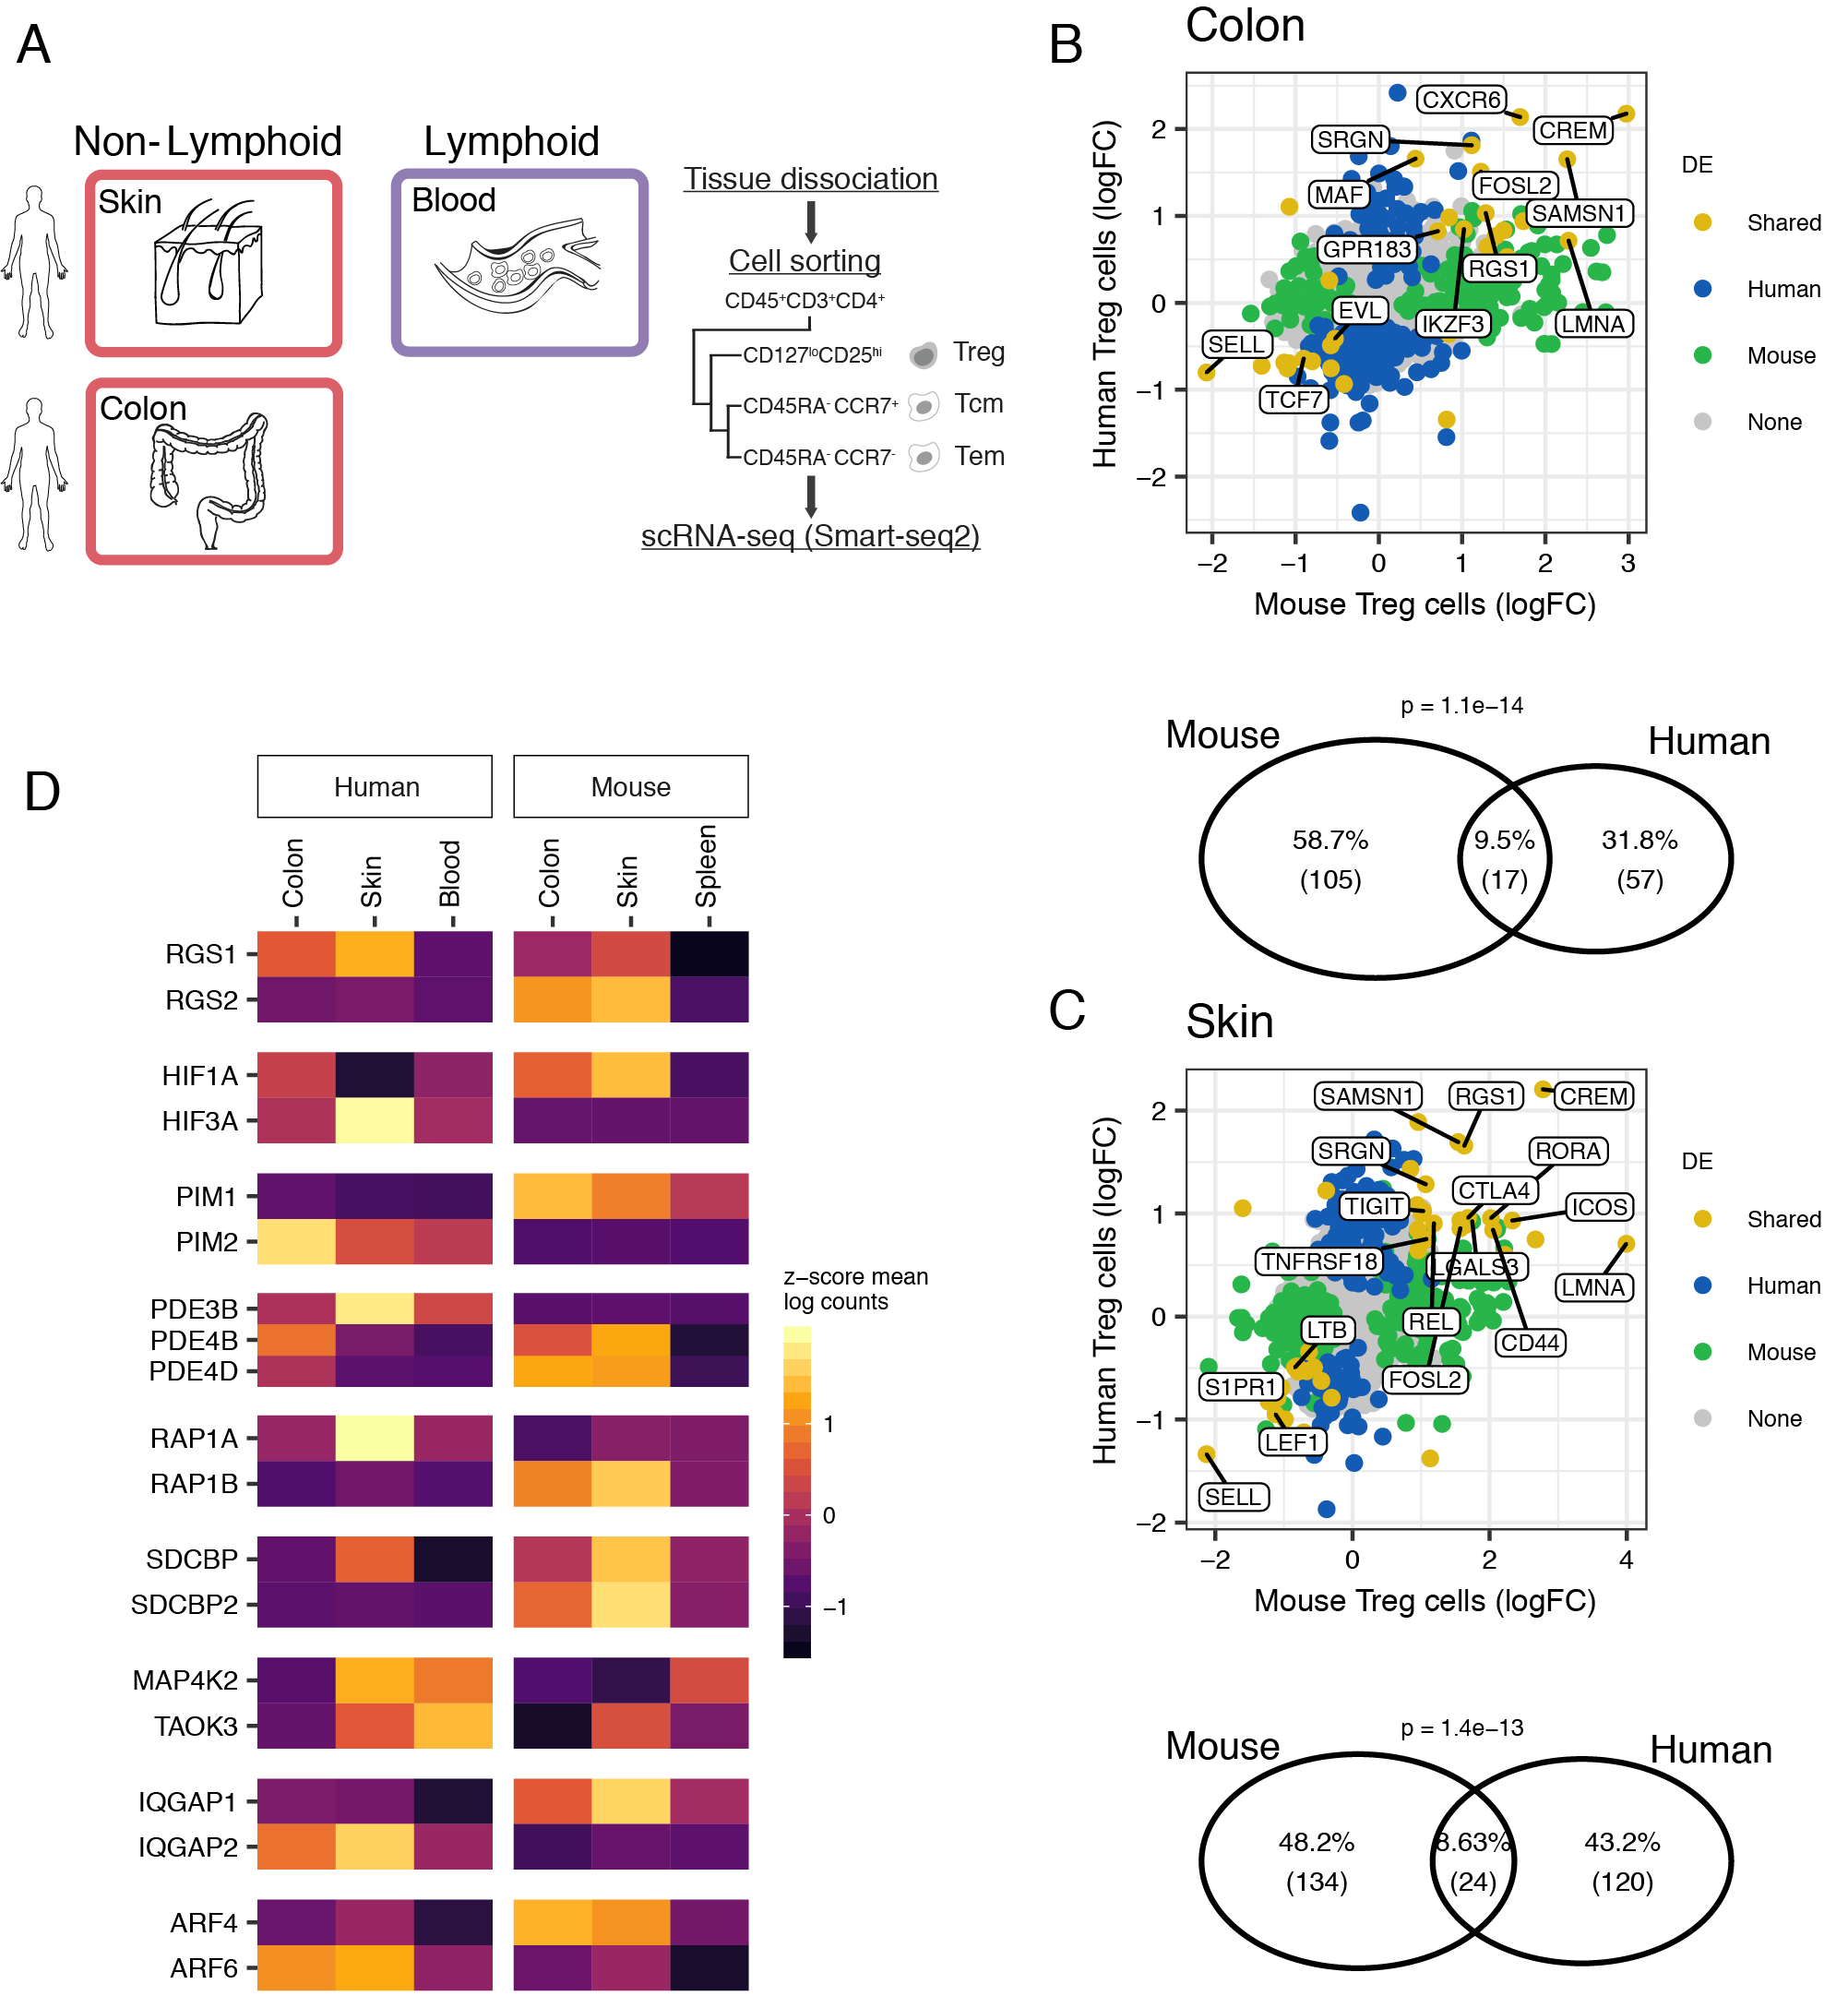
\includegraphics[width=1.0\textwidth]{Chapter2/Figs/chap2_fig5.png} % change word in curlies to change figure
\caption[Human-mouse comparison of NLT Treg cell marker genes.]{\textbf{Human-mouse comparison of NLT Treg cell marker genes.}\newline\textbf{(A)} Tissues and cell types sampled from human. \textbf{(B and C)} Top: Overlap between NLT Treg cell markers detected in human and mouse, in either (B) colon or (C) skin datasets. Bottom: Fold-change between gene expression in non-lymphoid and lymphoid tissues in mouse and human. Blood and spleen were used as lymphoid tissues in human and mouse respectively. \textbf{(D)} NLT paralogs exhibiting opposing expression patterns between human and mouse. See also Figure~\ref{fig:appA_fig6}.}
\label{fig:chap2_fig5}
\end{figure}

We complemented our characterisation of murine NLT Treg and Tmem cells by collecting human Treg cells, as well as Tmem (sorted into central and effector memory) cells from blood and skin, and from tumour-adjacent colon sections from patients undergoing colonic resection (Figure~\ref{fig:chap2_fig5}A, Figure~\ref{fig:appA_fig6}). Similar to the mouse analysis, we identified gene markers for human CD4\textsuperscript{+} T cell populations (see Methods).

Focusing on one-to-one orthologs, we found that 24 out of 144 human skin Treg cell markers and 17 out of 74 human colon Treg cell markers overlapped with the respective mouse signature. In colon, we observe the conservation of \textit{Tnfrsf4}, \textit{Lgals1}, \textit{Srgn}, \textit{Cxcr6}, \textit{Maf}, or \textit{Ikzf3} (Figure~\ref{fig:chap2_fig5}B), genes that we had previously identified as important in defining tissue identity and Treg cell subpopulations. The same applied to skin Treg cells, where we saw expression of \textit{Batf}, \textit{Rora}, \textit{Rel}, \textit{Srgn}, \textit{Tnfrsf18}, and \textit{Tigit} across species (Figure~\ref{fig:chap2_fig5}C). Overall, this indicates a conserved role of the core NLT signature, namely the TNFRSF-NF-${\upkappa}$B-pathway.

In several instances we observed the expression pattern of one gene being substituted by a paralog in the other organism (Figure~\ref{fig:chap2_fig5}D). For example, while the kinase \textit{Pim1} is a marker of mouse NLT Treg cells, and was not expressed in human, the inverse was true of \textit{Pim2}. A similar situation was observed for \textit{Rgs1}-\textit{Rgs2}, \textit{Hif1a}-\textit{Hif3a} and others. This suggests that some paralogous proteins have evolved to substitute each other during evolution of NLT Treg cells in mammals. The fact that several of the identified cases are receptors related to signal transduction leads us to believe that evolution of cell-cell communication pathways owes some plasticity to differential paralog usage.

Our cross-species comparison suggests that despite cross-species differences, the NLT Treg cell adaptation program defined in mouse is generally conserved in human. 


\section{Classfication of Treg populations across species}
\label{section2.7}
The increase in the number of datasets from a variety of species enables the comparison of cell types between them. In the previous section, it was explained how the core NLT Treg cell programmes were conserved between mouse and human, based on one-to-one orthologs. This type of orthologs make up the majority of conserved genes between these species, but one-to-many and many-to-many orthologs can also have important roles in cell identity and function.

\begin{figure}[pt] 
\centering    
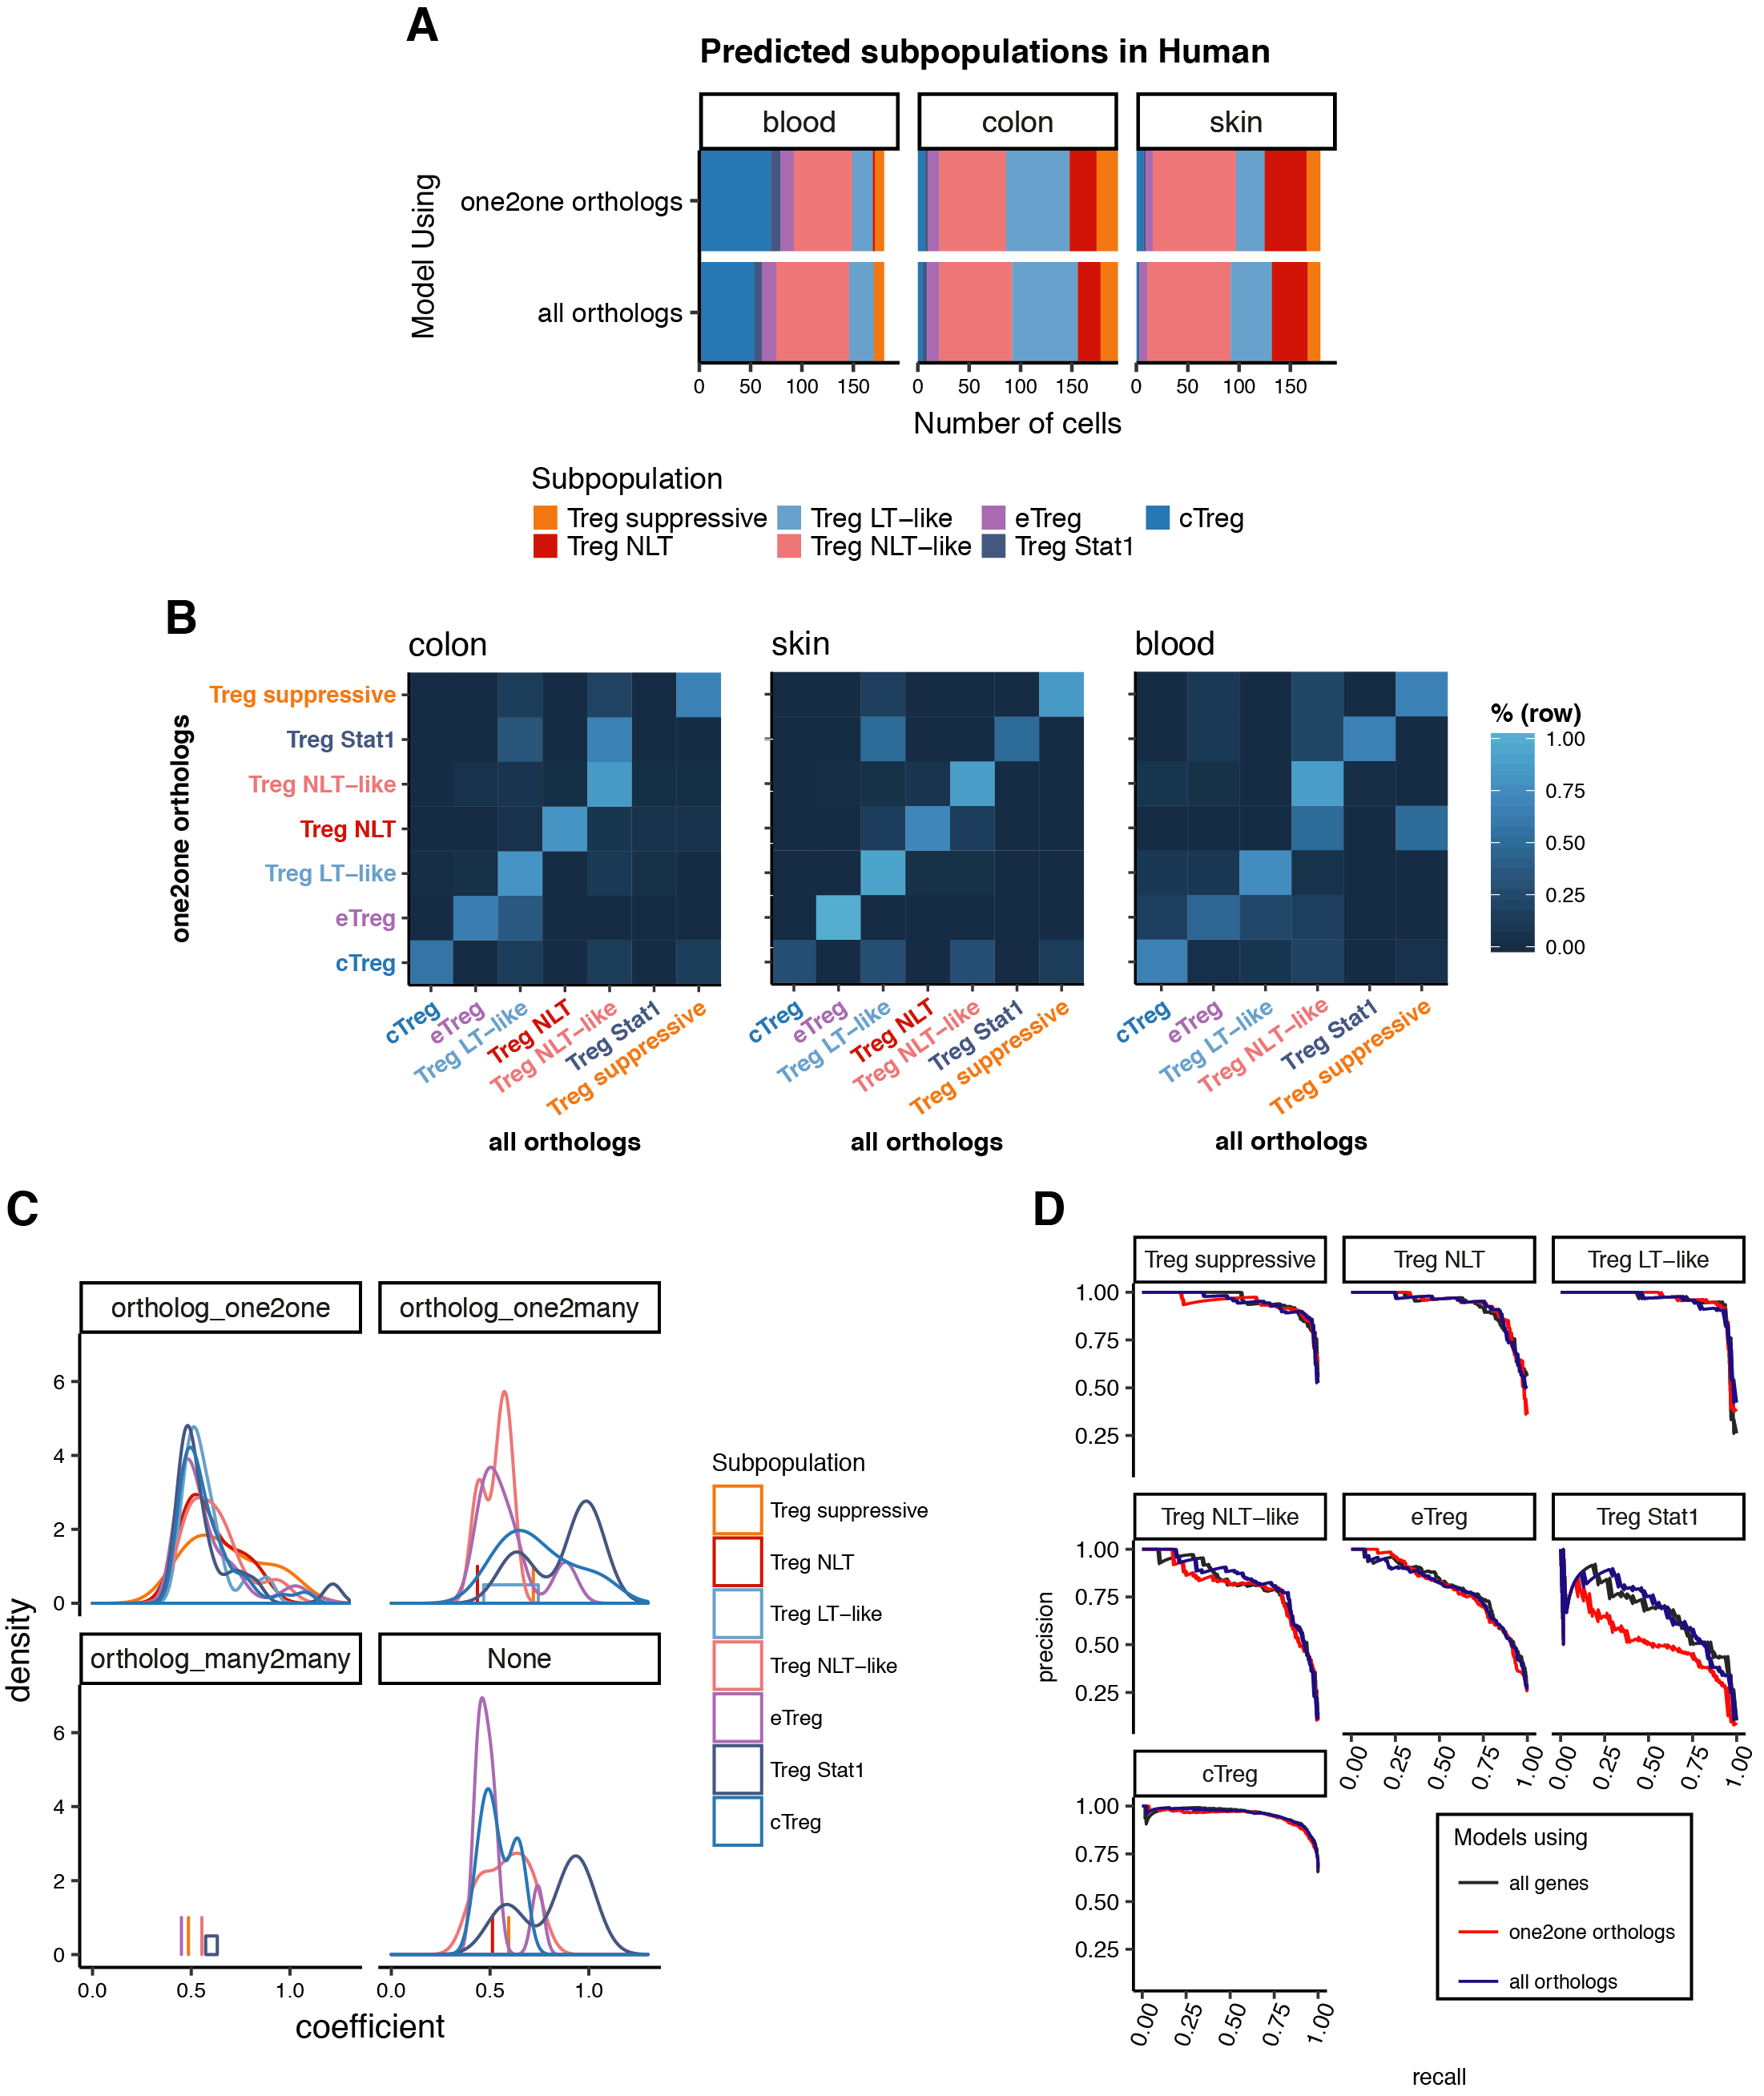
\includegraphics[width=1.0\textwidth]{Chapter2/Figs/chap2_fig6.png} % change word in curlies to change figure
\caption[Examining models for cross-species Treg classification]{\textbf{Training models for cross-species Treg classification.}\newline\textbf{(A)} Treg cells of each human tissue classified as each subpopulation detected in mouse using a logistic regression model trained with one-to-one orthologs (top) or all orthologs (bottom). \textbf{(B)} Row-normalised confusion matrices for each tissue, comparing the classifications using the one-to-one ortholog model (y-axis) against the all orthologs model (x-axis). \textbf{(C)} Distribution of the absolute value of coefficients for the top 300 genes learned for each population, in a model using all expressed mouse genes. \textbf{(D)} Precision-recall curves for models trained using all mouse genes, all orthologs or just one-to-one mouse-human orthologs. Precision and recall were calculated on a balanced test set composed of 10\% of mouse Treg cells.}
\label{fig:chap2_fig6}
\end{figure}

Two logistic regression models were trained to detect mouse Treg cell subpopulations in human cells (see Methods). The first model was trained solely using one-to-one orthologs expressed in both datasets. The second model included all genes with any sort of orthology by adding the counts of related genes. Within each tissue, predicted subpopulations appeared as expected, with blood containing more cTreg and eTreg cells than NLTs, which in their turn had more Treg NLT and suppressive cells (Figure~\ref{fig:chap2_fig6}A). Transition populations (Treg LT-like and NLT-like) appeared more represented in general, as well as present in both lymphoid and non-lymphoid tissues. This is an effect comparable to that observed in Figure~\ref{fig:chap2_fig2}G, where Treg NLT-like cells are shown to match Treg NLT or Treg LT-like cells from colon, likely because of the intermediate phenotype of the cells. 

When comparing the models per tissue (Figure~\ref{fig:chap2_fig6}A, top vs bottom row), similar subpopulation proportions are predicted per human tissue, indicating reduced differences between methods. However, we observe that the "one-to-one orthologs" model is the only that unexpectedly predicts the presence of Treg NLT in blood, and predicts in general a higher number of the rare, bLN-restricted Treg Stat1 subpopulation (Figure~\ref{fig:chap2_fig6}B). In the "all orthologs" model, cells that would be assigned to this subpopulation are instead distributed between Treg NLT-like or LT-like, which are more evidently present in the same tissues in mouse.

To examine the contribution of different types of genes for cell identity prediction, we used a model trained on all mouse genes, and plotted the genes with the top 300 coefficients in absolute value by subpopulation and orthology type (Figure~\ref{fig:chap2_fig6}C. This shows that, while different subpopulations have similar distributions of absolute coefficients for one-to-one ortholog genes, distributions for one-to-many orthologs (and genes with no listed ortholog) are more dissimilar. In particular, Treg Stat1 cells have a larger number of one-to-many ortholog genes with a higher coefficient than the remaining populations, underscoring the importance of this type of genes in defining this subset. Concomitantly, precision-recall curves calculated for a test set comprised of 10\% of mouse Treg shows that, while most subpopulations are equally well classified by both ortholog-based models, for Treg Stat1 cells only the "all orthologs" model performs as well as the "all genes" full model. These observations provide evidence that, while most cell states can be distinguished from one-to-one orthologs alone, this may not always be the case.


\section{Discussion}
\label{section2.8}
Our work sheds light on the phenotype of skin and colon Treg cells. We profiled NLT Treg and Tmem cells to identify global relationships between cell populations, discriminating general CD4\textsuperscript{+} and specific Treg cell markers in NLT. We found that these Treg populations conserve fundamental traits shared across the skin and colon compartments, namely a substantial prevalence of genes part of the TNFRSF-NF-${\upkappa}$B axis.
We leveraged the single-cell resolution of our data to explain Treg cell heterogeneity in the context of LT-to-NLT transition. Besides the eTreg cell state previously described in lymphoid organs~\citep{Cretney2011-zd}, we found two transitional subpopulations, Treg NLT-like cells in the lymphoid tissues and Treg LT-like cell in the non-lymphoid ones, which together explain the cross-tissue transition from central Treg to Treg NLT cell populations. NLT-like Treg cells in the mLN and bLN showed extensive NLT-priming, including the upregulation of tissue-specific homing-molecules to the drained NLT. Others have demonstrated that a subpopulation of spleen Treg cells can express a partial visceral adipose tissue (VAT) signature and later give rise to fully-mature VAT-Treg cells upon migration~\citep{Li2018-xq}, implying that this is valid for various tissues and should be considered in the design of future precision medicine strategies involving targeting of Treg cells to NLTs.

Our pseudotime results support migration and adaptation relationships between subpopulations, and allowed us to explore the basic mechanisms for the establishment of peripheral Treg cell phenotypes. In this transition, metabolic and proliferation changes in Treg cells happen concurrently with priming for migration, followed by changes in cytokine production machinery upon establishment in the periphery. Despite the overall similarity of recruitment and adaptation to NLTs, and although all three subpopulations (skin NLT, colon NLT, colon suppressive) fell close along the NLT adaptation trajectory, colon but mainly skin Treg NLT cells exhibited greater adaptation to the NLT environment. We hypothesise that the upregulation of \textit{Ikzf4}, \textit{Dgat2} and \textit{Itgae} observed in skin might explain and contribute to the further stabilisation, retention and metabolic adaptation of Treg cells to the NLT compartment.

Treg cell priming in LNs is apparent from their increased NLT signature and expression of tissue-homing molecules, yet it is likely that Treg NLT-like cells are a heterogeneous subpopulation, with some cells egressing to the NLTs and others recently drained from the NLTs. This was confirmed using velocyto, and agrees with the bidirectional migration between LNs and the NLTs described in skin using a photoconversion system~\citep{Matsushima2010-ph}. Studies coupling photoconversion and scRNA-seq can further our understanding of Treg cell migration patterns, as previously shown with single-cell qPCR~\citep{Ikebuchi2016-hb}.

A considerable proportion of the adaptation programme between bLN-to-tumour was contained within the bLN-to-skin trajectories. Similarly to steady-state, cues derived from NLTs are likely to prime Treg cells located in the draining LNs, as indicated by a higher percentage of cells expressing \textit{Batf}, \textit{Lgals1}, \textit{Id2} and other NLT markers in melanoma. In sum, tumour Treg cells resemble less mature versions of their homeostatic skin counterparts that, nevertheless, follow the same NLT adaptation trajectory.

The establishment of correct orthology relationships can be important for cross species comparisons. While we show that including a broader variety of ortholog genes improves prediction for one Treg subpopulation, this is not a definitive solution and should warrant further testing. A drawback still present is the exclusion of genes with no defined orthology relationship. These could be included by an approach that aggregated the genes by gene sets that would match between species, which can be agnostic to these evolutionary relationships and instead rely on per-species gene functional descriptions. It can however leave out less well studied genes, or have poorer performance for less well described or annotated species.

Despite the conserved tissue-specific signatures, the differential paralog usage identified between species (Figure~\ref{fig:chap2_fig5}D) suggests a pivotal role for expanded gene families in rewiring signalling pathways throughout evolution. Studies focusing not only on tissue-resident cells, but also on the surrounding environment and organs can help dissect the relevance of these pathways in T cell biology, and how this evolutionary rewiring might affect immune response and homeostasis.

Overall, we reveal a dynamic adaptation of T cells as they traffic across tissues, and provide an open resource (data.teichlab.org) for investigating \textit{in vivo} CD4\textsuperscript{+} T cell phenotypes in mouse and human, to ultimately harness NLT CD4\textsuperscript{+} T cells as future therapeutic targets.


\section{Methods}
\label{section2.9}

For further experimental methods see Appendix~\ref{appendix:treg}.

\subsection{RNA expression quantification and normalisation}
Sequencing data from 10x runs was aligned and quantified using the CellRanger software package with default parameters.

Gene expression from Smart-seq2 scRNA-seq data was quantified in counts using Salmon v0.6.0~\citep{Patro2017-ce}, with the parameters --fldMax 150000000 --fldMean 350 --fldSD 250 --numBootstraps 100 --biasCorrect --allowOrphans --useVBOpt. For mouse, the cDNA sequences used contain genes from GRCm38 and sequences from RepBase, as well as ERCC sequences and an EGFP sequence. Since the EGFP RNA is transcribed together with \textit{Foxp3}, counts from these two genes were added after quantification to represent \textit{Foxp3} expression. For human data quantification, cDNA sequences from GRCh38 and ERCC were used.

Standard scRNA-seq analysis (QC, differential expression and marker gene detection, and clustering) was performed using Seurat~\citep{Satija2015-ti}. All data was log-normalised using the NormaliseData function with a scale factor of 10000. Our expression data for different tissues is also available for user-friendly interactive browsing online at data.teichlab.org.

\subsection{scRNA-seq quality control}
Quality control of 10x-derived data was made taking into account number of UMIs - keeping cells with between 1000 and 15000 UMI - and number of genes - keeping cells with between 700 and 3500 genes with at least 1 UMI (Table S1). While cells were not filtered by their mitochondrial read content, cells with an elevated number of these reads are eventually removed via clustering (see “Subpopulation detection in 10x data”).

For Smart-seq2 data, count values for each cell were grouped in an expression matrix, and ERCC expression were separated from true gene expression. Cells were then filtered based on different quality parameters calculated for each dataset (Table S1). Additionally, the output of TraCeR~\citep{stubbington_t_2016} was used to remove cells without a detected TCR sequence, as well as invariant Natural Killer T (iNKT) cells and ${\upgamma\updelta}$ T cells (defined as cells with at least one ${\upgamma}$ and one ${\updelta}$ chain detected and no ${\upalpha\upbeta}$ pair). For the colon and skin datasets, 433 and 745 cells passed quality control, respectively.

Importantly, we note that TCR detection greatly improved our filtering by excluding cell types captured by FACS that did not fit the intended categories. This is the case for iNKT cells - captured mostly together with spleen T memory cells - and ${\upgamma\updelta}$-T cells - sorted together with skin Tmem cells in the melanoma experiment. Indeed, we also identified a NKT population in the 10x dataset, mostly within the cells sorted as spleen Tmem cells, as well as some LN Tmem cells (Figure~\ref{fig:appA_fig1}B and~\ref{fig:appA_fig1}C). We cannot, however, state that these are “invariant”, since we have no access to their complete TCR chains. TCR filtering also enables removal of cell doublets by identifying cells expressing an excessive diversity of recombined TCR chains. Even in cases of no allelic exclusion for TCR ${\upalpha}$ and ${\upbeta}$ sequences, each cell would still only be able to produce two recombinants of each, allowing removal of cell doublets expressing more than two recombinants for a TCR locus. Lastly, we removed all cells not expressing any recombinant TCR in order to have a more stringent quality control. While in the human dataset the number of cells without a TCR was evenly distributed across tissues and cell types, there was a clear skew towards TCR absence in peripheral Treg cells (colon and skin) in the mouse datasets. These Treg cells did not appear to differ from the remaining population, having no differentially expressed genes or major differences in their overall number, presenting only a skew towards a higher number of reads (data not shown).

\subsection{Dimensionality reduction methods}
To obtain an overview of the datasets showing the relationships between cell population clusters, Principal Component Analysis (PCA) and tSNE were used. Before PCA, data was scaled using the ScaleData function (negative binomial model, normalising by the number of UMI and centering the data). PCA and tSNE were calculated using the RunPCA and RunTSNE functions, respectively. For each dataset, a different number of Principal Components (PCs) and values for perplexity were used (Table S1), chosen by visual inspection of an elbow plot representing the relative importance of each PC. With exception of the PCA projection for the complete 10x dataset, only highly variable genes were used, calculated using the FindVariableGenes function from Seurat with the parameters num.bin=100 and binning.method="equal${\_}$frequency". Using all genes for dimensionality reduction of the whole 10x dataset resulted in more accurate clustering, allowing for the identification of most contaminant cells on this first step (Figure~\ref{fig:appA_fig1}B). Plate-based datasets were treated separately as much as possible to avoid confounding batch effects from experiments performed separately.

\subsection{Subpopulation detection in 10x data}
To find clusters in the data, we used the FindClusters function from Seurat, with the same number of principal components used for tSNE. Cluster annotation was done by inspecting markers detected by the FindAllMarkers function.

Global clustering of the 10x dataset was done with the resolution parameter set to 0.2. After clustering the complete dataset, we excluded artifactual subpopulations (Figure~\ref{fig:appA_fig1}, Table S2). A mixed Treg and Tmem cell population characterised by high expression of immediate-early response genes (e.g. Jun, Junb, Fos, Fosb), which has previously been reported in other cell types~\citep{Adam2017-wd,Van_den_Brink2017-lg,Wu2017-jn} was removed. An additional population of lymphoid tissue Tmem cells was also excluded because they presented expression profiles similar to NKT cells (\textit{Nkg7}, \textit{Ccl5}, \textit{Cd160}, \textit{Klrbc1}, \textit{Cxcr6}).

Clustering on individual tissues used the following resolutions: for Treg cells, 0.3 on Spleen, 0.4 on bLN, 0.4 on mLN, 0.5 on Colon, 0.4 on all skin cells; for Tmem cells 0.4 on Spleen, 0.3 on bLN, 0.7 on mLN, and 0.6 on Colon. Annotation was performed and subpopulations characterised by immediate-early response genes were removed (Table S3).

\subsection{Differential expression analysis}
Differential expression (DE) and marker gene detection was performed using the FindMarkers and the FindaAllMarkers functions from the Seurat R package, using the default Wilcoxon test. Genes were considered differentially expressed if they had an average log fold-change of at least 0.25 and a Bonferroni-adjusted p-value of 0.05 or lower. 

For DE including all cells of the 10x dataset, a minimum of 5${\%}$ of cells had to express the gene, otherwise a minimum of 1${\%}$ was used. For comparisons between tests (for example Treg vs Tmem cells and LT vs NLT, see Figure~\ref{fig:chap2_fig1}C), the FindMarkers function was run twice - the first time to determine all genes considered expressed for each comparison, the second using the union of all those genes.

In the human and mouse comparison, human NLTs were compared to blood and mouse NLTs were compared to spleen only, and testing was restricted to genes with one-to-one orthologs.

\subsection{Mapping cells to known populations using logistic regression classification}
To make a correspondence of cells in the 10x dataset with the identified Treg cell subtypes in the colon (Figure~\ref{fig:chap2_fig2}G), or between Smart-seq2 data and the complete 10x dataset (Figure~\ref{fig:appA_fig2}B), the counts and subpopulation labels of the 10x dataset Treg cell subpopulations and the complete 10x dataset were used to train a logistic regression classification model using scikit-learn with an L1 penalty and default parameters. The label with the highest probability predicted by the model was then attributed to each cell. The figures show the percentage of each tested population that was predicted as matching to each learned label.

For cross-species mapping of Treg subpopulations, 90\% of the sorted Treg cells from mouse were used to construct two models, with the remaining subpopulation-balanced partition kept separately for model testing. The first model (refered to in Figure~\ref{fig:chap2_fig6} as "one-to-one orthologs") was used only using genes expressed in both species that are one-to-one orthologs. Another model was trained by using all genes with known orthologs, and adding the counts for genes with many orthologs. For example, if a gene in mouse corresponds to three genes in human (i.e. a one-to-many relationship), then the counts of the three human genes are added and given one identifier. For many-to-many relationships, the same happens in both species simultaneously. Additionally, a third model was trained using all mouse genes, to use as a ground truth for the predictive power of the other models. With 10-fold cross validation, these three models have a mean accuracy of 84.0\%, 84.7\%, and 85.6\%, respectively. Precision-recall curves were then calculated using the 10\% test set.

\subsection{Obtaining a migration latent variable for steady-state Treg cells}
The large dimensionality of single-cell RNA-seq data has been used before to gain insights on time-dependent events~\citep{trapnell_dynamics_2014,lonnberg_single-cell_2017} by applying methods for pseudotime inference. Although it is impossible to follow one cell through the complete process, these methods can order single-cell data into a continuous dimension, using the discrete samples as snapshots containing a multitude of intermediate states.

Immune cells are expected to migrate between LTs and NLTs. We assumed that this effect would be reflected as a gradual single-cell expression phenotype, which could be captured as a latent variable of the data. To achieve this, we used Bayesian Gaussian Process Latent Variable Modelling (BGPLVM)~\citep{Michalis_K_Titsias2010-na}, implemented in the python package GPy (https://github.com/SheffieldML/GPy) as “GPy.models.BayesianGPLVM”, which was already used before for dimensionality reduction in scRNA-seq data to model Th1-Tfh cell differentiation~\citep{lonnberg_single-cell_2017}. BGPLVM was used on log-scaled counts and only considering highly variable genes. We run the method with six latent variables (LV) to be sure we capture the most relevant ones by Automatic Relevance Determination (ARD, Figure~\ref{fig:appA_fig3}A), although this number does not alter significantly the performance of the algorithm. We then interpret the most important LV as the one ordering the cells between tissues along a migration and adaptation transition. In agreement, we observe gene expression changes associated with losing the lymphoid tissue identity and acquiring a peripheral tissue transcriptional profile (Figure~\ref{fig:chap2_fig3}B).

For 10x data, the method was used on mLN and colon Treg cells. We then mapped bLN and skin Treg cells onto the same LV using the predict function from the BGPLVM module, in order to have a similar coordinate system for both trajectories. Running BGPLVM with all data together would achieve a similar result (not shown). A BGPLVM projection of bLN and skin Treg cells (Figure~\ref{fig:appA_fig3}B) shows an identical projection but with a wider gap between bLN and skin cells due to the large differences in cell numbers. We excluded spleen cells from this analysis to focus specifically on LN to NLT adaptation.

Similar effects are also observed in the corresponding Smart-seq2 cells (Figure~\ref{fig:appA_fig4}D). We then show that all the LVs chosen as a “pseudospace variable” (LV0) have a similar effect between datasets by comparing the shared proportions of genes correlated with each of them (Figure~\ref{fig:appA_fig4}E). 

\subsection{Identifying a common tissue migration trajectory in control and melanoma}
Similarly to the steady-state, migration from the LN to the skin with a melanoma challenge is also expected. A common between-tissue Treg cell migration trajectory in control and melanoma conditions was obtained using Manifold Relevance Determination~\citep{Andreas_Damianou_Carl_Ek_Michalis_Titsias_Neil_Lawrence2012-do} (MRD). MRD works by having an underlying BGPLVM model whose dimensions can be shared or private between sections of the data. Having the prior knowledge that a cell-cycle effect is present in the data (Figure~\ref{fig:appA_fig5}A) and with the goal of obtaining a LV explaining tissue recruitment in both conditions, the melanoma dataset was divided into three sections for input: one with the expression in all cell-cycle associated genes, one with marker genes for any tissue, and one with the remaining genes. The importance of each section in each latent variable is shown in the ARD plot (Figure~\ref{fig:appA_fig5}C). The model was run allowing for 12 LVs as output, and the one highly influenced by tissue-specific genes but not cell-cycle or other genes was used as a migration trajectory for both conditions (Figure~\ref{fig:chap2_fig4}D). The effects captured by these LVs can be observed in BGPLVM projections for the individual conditions (Figure~\ref{fig:appA_fig5}E-G).

\subsection{Switch-like genes in the migration latent variable}
Gene expression changes in a continuous trajectory can be interpreted as a series of switch-like events. These can be modeled using a sigmoid curve, described by the following equation:

\begin{align}
S = \frac{2 x \mu_0}{1 + \mathrm{e}^{-k(t - t_0)}}
\end{align}

where ${\upmu\textsubscript{0}}$ is the mean expression between the sigmoid “on” and “off” states, t\textsubscript{0} is the point in which the switch in expression happens, and k defines the sigmoid inclination and can be interpreted as the activation strength. Parameter k will additionally inform on the direction of the switch (activation or inhibition) from its signal.

The R package switchde~\citep{Campbell2017-cf} was used to model gene expression as a sigmoid in the inferred migration trajectories, using the appropriate latent variable as pseudotime. 

In the steady-state 10x dataset partitions (mLN+colon Treg cells and bLN+skin Treg cells), switchde was applied for non-Tmem cell specific genes expressed in at least 30 cells, as well as genes with an absolute correlation greater than 0.25 with the LV chosen for both partitions. Due to the large differences in the number of cells in the skin partition, we ran switchde 100 times on different subsamples of each Treg cell subpopulation matching the smallest subpopulation size (405 for the colon partition, 55 for the skin partition), and used the median values of the parameters for further analysis. For the melanoma dataset, genes expressed in at least 5 cells in both conditions were tested. Only genes with a q-value<=0.05 and that had a t\textsubscript{0} within the LV range were kept for further interpretation.

\subsection{RNA velocity estimation}
RNA velocity is a measure that leverages detection of spliced and unspliced transcripts to predict single-cell development directionality ~\citep{manno_rna_2018}. We used velocyto to determine in which direction cells were changing in the cross-tissue adaptation trajectories. We have followed the python implementation of velocyto, and the code can be found in \url{https://github.com/tomasgomes/Treg\_analysis/blob/master/Velocyto.ipynb}, where each of the runs is present.

\subsection{Detection of expanded clonotypes}
T cell receptor (TCR) sequences were reconstructed from single-cell RNA-seq data and used to infer clonality using TraCeR~\citep{stubbington_t_2016}. We used TraCeR with the parameters --loci A B D G, --max\_junc\_len 120 to allow reconstruction of TCR${\upalpha}$, TCR${\upbeta}$, TCR${\updelta}$ and TCR${\upgamma}$ chains in each cell and to permit TCR${\upgamma}$ chains with long CDR3 regions. 

\subsection{GO Term enrichment}
To test for enriched GO Biological Processes or KEGG Pathways in gene sets, the gprofiler R package~\citep{Reimand2016-fj} was used, with the option of moderate hierarchical filtering enabled.
To determine the succession of Biological Processes GO Terms (Figure~\ref{fig:chap2_fig3}C, Table S4), we used the approach above on all genes called DE by switchde, and plotted only the terms with at least two genes.

\subsection{Cell-cycle analysis}
To assess potential effects of cell-cycle in the interpretation of the scRNA-seq datasets, Cyclone~\citep{Scialdone2015-tw} (implemented in the scran R package) was used on all datasets. Results for the mouse melanoma dataset (where a relevant cycling population exists) were projected on the tSNE (Figure~\ref{fig:appA_fig5}A). As the vast majority of cells was assigned to the default cell-cycle stage (G0/G1 in mouse, S in human), no cell-cycle correction was performed.

%!TEX root = ../thesis.tex
%*******************************************************************************
%****************************** Third Chapter **********************************
%*******************************************************************************
\chapter{Developing an integrated reference for automatic cell type annotation} \label{chap:CT_method}

% **************************** Define Graphics Path **************************
\ifpdf
    \graphicspath{{Chapter3/Figs/Raster/}{Chapter3/Figs/PDF/}{Chapter3/Figs/}}
\else
    \graphicspath{{Chapter3/Figs/Vector/}{Chapter3/Figs/}}
\fi
The widespread adoption of single-cell sequencing technologies has revolutionised the molecular profiling of cells. The use of these methods allows us to understand the building blocks of tissues at an unprecedented resolution. As further human tissues are examined, a catalog of cell types and their gene expression profile can be compiled from published data. Such compilation, covering a broad variety of organs and obtained using different methodologies, can provide a reference to which newly collected data can be compared for immediate annotation, while in parallel revealing the underlying relationships between cell populations across the organism.

This chapter outlines the development of \textit{CellTypist} - an integrative reference of cell types based on single-cell transcriptomic data. The \textit{CellTypist} pipeline relies on predictive models to integrate data from different sources, and allows for automatic and unbiased annotation of scRNA-seq datasets. Additionally, integration of data from numerous sources can inform on cell type similarity, and thus serve as a framework for an expression-based cell type ontology.

This project was initially conceived together with Valentine Svensson while he was part of the Teichmann group. The pipeline here outlined serves as the basis for the analyses performed in Chapter~\ref{chap:CT_bio}.


\section{Introduction}
\label{section3.1}
% cataloguing all cell types
The aim of classifying and characterising all different types of cells that compose the various anatomical regions has been present ever since it was first postulated that all living organisms are composed of cells~\citep{schwann_microscopical_1847}. For the greater part of the history of cell biology, cells have been characterised and identified based on their physical appearance~\citep{mazzarello_unifying_1999}. The development of immunohistochemistry~\citep{coons_immunological_1941}, and later its combination with the large throughput provided by flow cytometry and FACS~\citep{hulett_cell_1969,bonner_fluorescence_1972}, started the current trend of molecular definition of cell types. More recently, developments in single-cell sequencing have enabled unbiased and high-throughput assessment of cell types through transcriptomic profiling~\citep{svensson_exponential_2018}. A few individual works have aimed at profiling cell types across most tissues of an organism~\citep{fincher_cell_2018,plass_cell_2018,han_mapping_2018,noauthor_single-cell_2018}. Other more complex and detailed cellular census have been done for individual tissues, and large consortia have been established to aggregate some of these datasets and establish guidelines and collaborations to identify all cell types across an organism~\citep{regev_human_2017}.

% integration methods, classification methods, comparison
Individually, studies using scRNA-seq have provided crucial insights into cell biology. Nonetheless, the data generated can often be reused for new purposes, either on its own to extract new conclusions, or through combination or comparison with novel data. To combine scRNA-seq datasets, batch correction and batch alignment methods seek to either correct gene expression values accounting for technical metadata~\citep{ritchie_limma_2015,johnson_adjusting_2007,buettner_f-sclvm:_2017,haghverdi_batch_2018,buttner_test_2019}, or place cells from different batches, technologies and datasets in a common manifold, allowing joint clustering and pseudotime analysis~\citep{butler_integrating_2018,polanski_bbknn:_2019,hie_efficient_2019,korsunsky_fast_2018,stuart_comprehensive_2019}. Conversely, comparison between scRNA-seq datasets aims to impart the knowledge gained from one dataset into another, usually through classification models. Various methods have been developed to compare cell types (and indeed other labels) across datasets (reviewed in Chapter~\ref{section1.3}, Table~\ref{table:tab_1_2}). Nonetheless, while these tools are highly effective at annotating new data using specific datasets, their scope will be limited to the dataset chosen as a reference.

% short description of the chapter
%% mention nomenclature: cell types - prior annotation; clusters - any derived, not named labelling. CellTypist, by default, uses CLUSTERS
To address the need for a reference that can allow fast and automatic annotation across tissues, we have developed \textit{CellTypist}, a pipeline for integration and classification based on logistic regression classifiers. Providing this pipeline with a broad collection of datasets creates an unbiased cell identity reference to be used in novel datasets. While previous work has been developed for well annotated mouse data  using a neural network-based classifier~\citep{alavi_web_2018}, \textit{CellTypist} can leverage data with different levels of annotation, focusing on providing broad identifiers for cells based on a reference from pooled data.

\begin{figure}[ht!]
    \centering    
    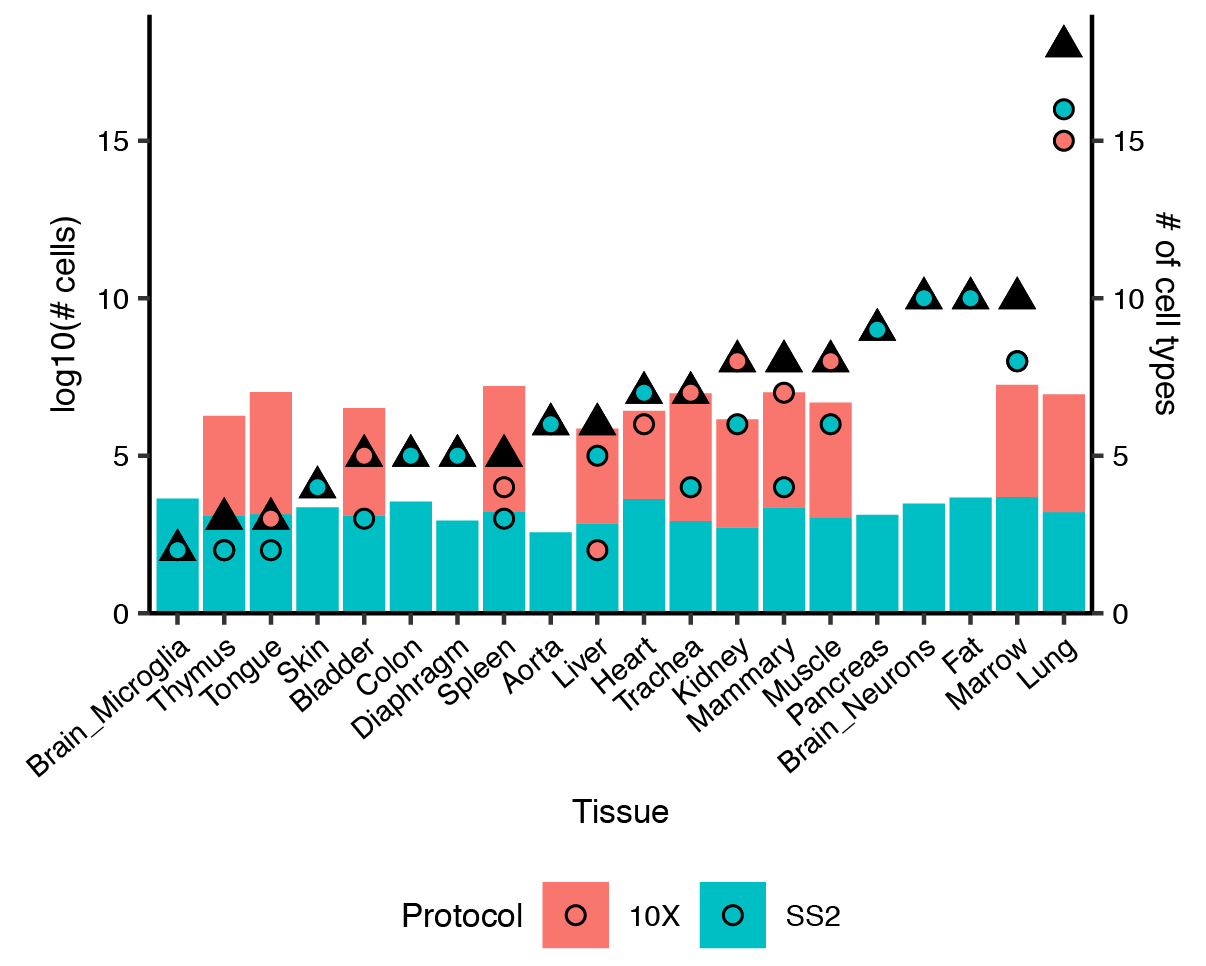
\includegraphics[width=1.0\textwidth]{Chapter3/Figs/countsCTCells_TabulaMuris.png} % change word in curlies to change figure
    \caption[Cell numbers in the \textit{Tabula Muris} dataset]{\textbf{Cell numbers in the \textit{Tabula Muris} dataset} \newline Bars show number of cells (left y axis) collected from different tissues (x axis), split by scRNA-seq protocol (colour). Points show the number of cell types (right y axis) identified by protocol (coloured circles) or their union (triangle). 10X - Chromium (10X Genomics) protocol; SS2 - Smart-seq2 protocol.}
    \label{fig:chap3_tmcounts}
\end{figure}

This chapter discusses the organisation of the \textit{CellTypist} pipeline, and explores its strengths and caveats. Evaluation of the pipeline will be performed on the \textit{Tabula Muris} data~\citep{noauthor_single-cell_2018}, summarised in Figure~\ref{fig:chap3_tmcounts}. Despite coming from a sole publication, this dataset has the advantage that it was generated in highly controlled conditions, spans 20 tissues, and includes a detailed and robust cell type annotation to which the clusters that result from integration using \textit{CellTypist} can be compared. The next Chapter will further explore the biological insights extracted from a collection of published human data from various sources, and how it can be used to interpret new data.


\nomenclature[z-SS2]{SS2}{Smart-seq2}

\section{Methodology and Results}
\label{section3.2}
\subsection{per-tissue clustering and cell type comparison}
\label{section3.2.1}
Reference data processing with \textit{CellTypist} follows three major steps. First, the data collected follows a procedure for uniform per-tissue processing (Figure~\ref{fig:chap3_pertiss}A). Next, the clusters determined in each tissue are matched across the whole dataset (Figure~\ref{fig:chap3_combcl}A). Lastly, the combined clusters are used as labels to train a logistic regression classifier using the complete data collection (Figure~\ref{fig:chap3_model}A).

Most studies using scRNA-seq profile cellular heterogeneity in a given biological sample, which often results in reporting the cell types or cell states present. While this is clearly displayed in the figures from these studies, this information in not always supplied in a machine-readable format, associated with either the raw sequencing reads or the quantified gene expression. Furthermore, most annotations do not follow a uniform, controlled vocabulary~\citep{bard_ontology_2005}, and is often done at varying resolutions depending on the focus of the study or the breadth of the dataset.

\textit{CellTypist} starts by splitting the collected data by tissues, grouping together data from different studies that profile the same body part, even if using distinct scRNA-seq protocols (Figure~\ref{fig:chap3_pertiss}A). At this stage, data from each tissue is processed following a uniform workflow using scanpy~\citep{wolf_scanpy:_2018}. Gene expression counts are normalised, and different datasets are batch aligned using BBKNN~\citep{polanski_bbknn:_2019} - in \textit{Tabula Muris}, different protocols are treated as independent data. Lastly, clustering at varying resolutions using the Leiden algorithm~\citep{traag_louvain_2019} is performed. This processing is executed to ensure that all tissues are similarly treated, regardless of the level of annotation, and to allow unannotated data to be included and bolster \textit{CellTypist}'s training data.

\begin{figure}[pht!]
    \centering    
    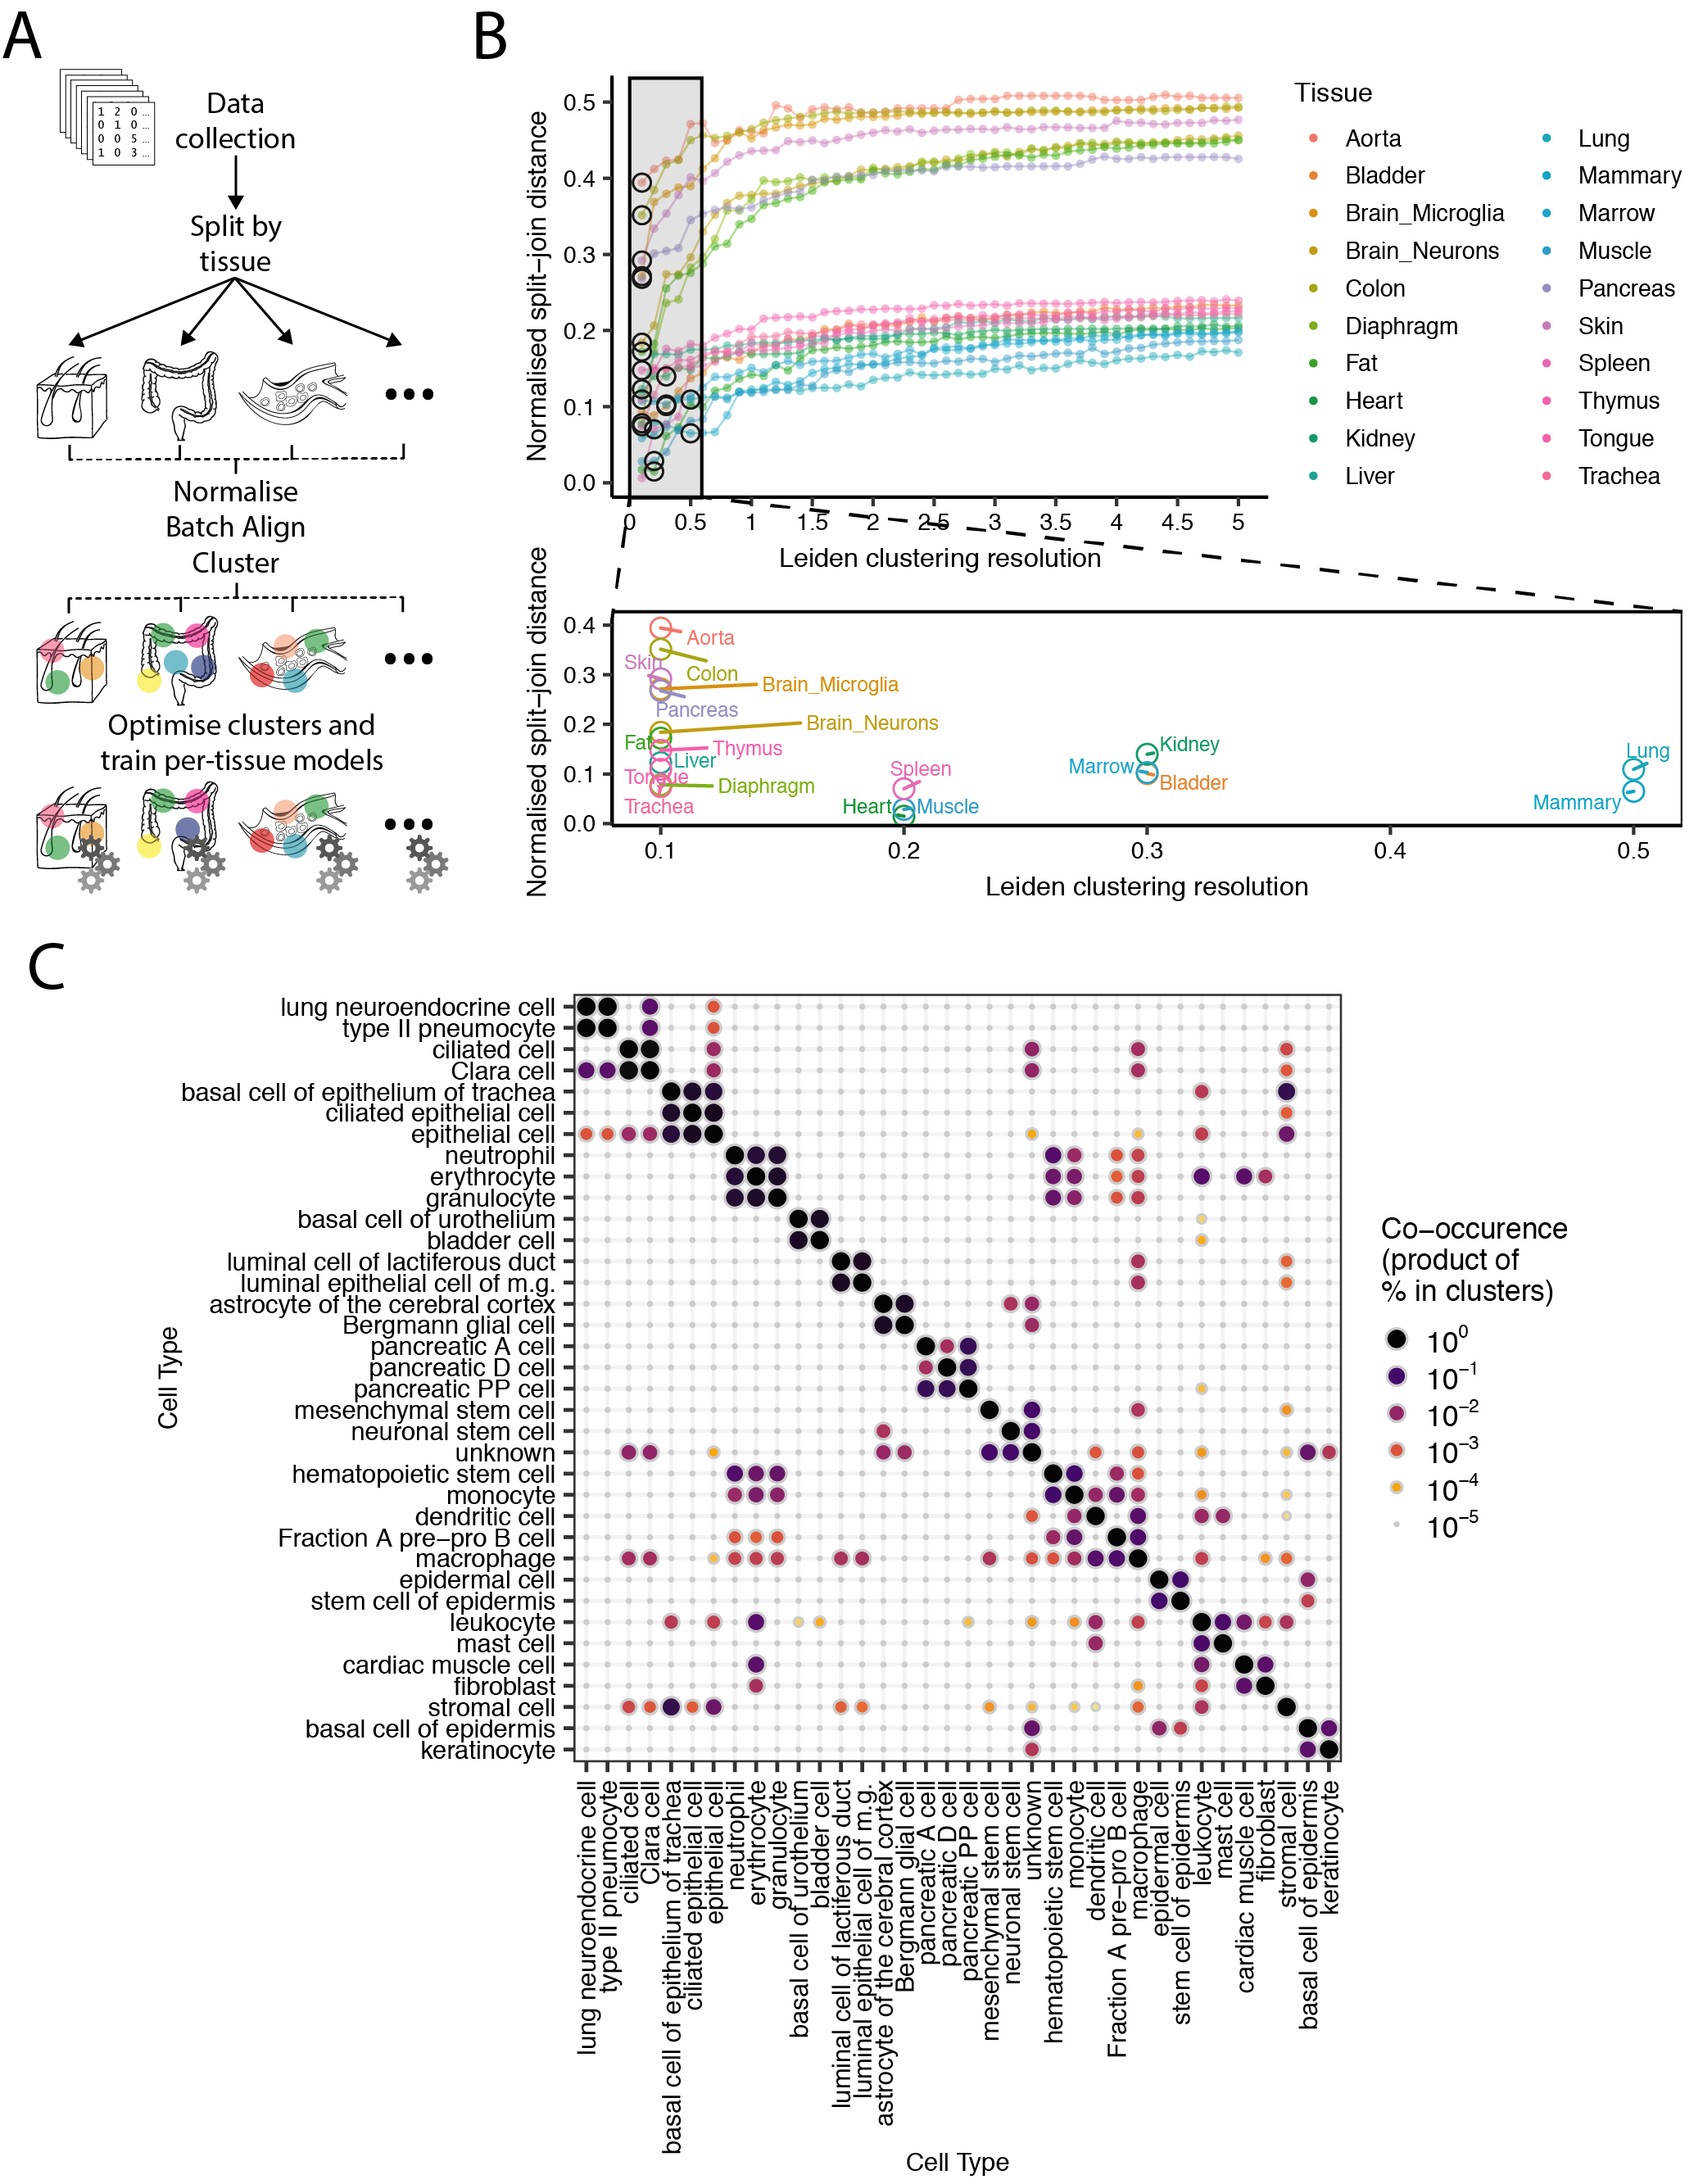
\includegraphics[width=1.0\textwidth]{Chapter3/Figs/chap3_TMperTissue.png} % change word in curlies to change figure
    \caption[Data reprocessing per-tissue]{\textbf{Data reprocessing per-tissue}\newline\textbf{(A)} Pipeline for initial data processing. Data collected is split into tissue, followed by integration of different datasets (in \textit{Tabula Muris}, different protocols), and clustered to optimally match existing cell type annotations. (Continued on the following page.)}
    \label{fig:chap3_pertiss}
\end{figure}
\begin{figure}[t]
  \contcaption{(continued) \textbf{(B)} Per-tissue cluster optimisation, choosing the resolution that approximates existing cell type annotations. Similarity is measured with normalised split-join distance, and constrained to solutions with a number of clusters of at least as many as existing annotations in the tissue. Upper panel shows the full range of resolutions tested per-tissue; lower panel shows the resolution range in which the optimal value for each tissue was present. \textbf{(C)} Co-occurrence of annotated cell types in the same clusters, determined by summing the products of each cell types per-cluster percentage. Only cell types with at least one co-occurrence value of 0.05 were kept. m.g. - mammary gland.}% Continued caption
\end{figure}

% explain SJ
Per-tissue clustering can be optimised to approximate existing cell type labels. To this end, clusters from each tissue were generated using a range of values for the resolution parameter of the Leiden algorithm. The clusters obtained were subsequently compared to known cell type annotations, and the resolution that is the closest and generates at least the same number of groupings was kept for the subsequent stages (Figure~\ref{fig:chap3_pertiss}B, top). Distance between clusters and cell types was calculated using the normalised split-join distance~\citep{dongen_performance_2000}. Briefly, the split-join metric measures the distance between two data partitions according to the number of element-wise division (split) or merge (join) operations necessary to fully convert the new partition into the former. In this specific example, it counts the number of operations necessary to convert the new cluster back into the known cell type annotations. Since the values in the original metric are dependent on the number of elements being cluster, and which here differ between tissues, Figure~\ref{fig:chap3_pertiss}B shows a normalised version of the metric, where it was divided by 2N, with N = number of cells for a given tissue.

Despite the broad range of clustering resolutions tested, (from 0.1 to 5 at 0.1 intervals), the parameters chosen for all tissues concentrated at resolutions of up to 0.5 (Figure~\ref{fig:chap3_pertiss}B, top shaded box and bottom expansion). Tissues appeared to organise into two distinct groups: a smaller group with a split-join distance above 0.2, and a larger one with a distance below 0.2. Interestingly, all tissues in the first group were only sequenced using Smart-seq2 (Figure~\ref{fig:chap3_tmcounts}), suggesting that integration of data from different protocols is not resulting in clusters that incorrectly approximate known cell types. The group with the higher distance had, in general, fewer cell types annotated, thus the higher values could be explained by tissue overclustering.

To gain a deeper insight into the performance of the per-tissue clustering step, co-clustering of known cell types was examined across all tissues (Figure~\ref{fig:chap3_pertiss}C). We started with a cell type-by-cluster matrix, showing the distribution of cell types per cluster as a percentage. To obtain a symmetric matrix, i.e. show the co-occurrence of two cell types normalised for the occurrence of each cell type, we obtained the product of this matrix with its transposed form. The resulting matrix is subsequently filtered to only include cell types with at least one co-occurrence value of 0.05 (meaning more than 20\% of the cells from each cell type in a pair would appear in the same clusters). Besides a high clustering of cells with the same annotation, the plot shows that most of the mixing happens between related cell types (e.g. epithelial cell, ciliated epithelial cell and basal cell of epithelium of trachea; luminal cell of lactiferous duct and luminal epithelial cell of mammary gland), or between hematopoietic-derived cells (e.g. neutrophil, erythrocyte, granulocyte; hematopoietic stem cell, macrophage and dendritic cell; leukocyte and mast cell). This is expected due to the similarities between related cell types, as well as due to less resolved clustering of immune and non-immune cells when these are analysed together. Another possible explanation is the existence of doublets, yet these tend to happen between specific pairs of cell types, which was not the most common case.

Overall, despite some losses in the resolution of cell groupings, the per-tissue clustering step of \textit{CellTypist} maintains much of the cell type information existing in the original data.


\subsection{Cross-tissue cluster combination}
\label{section3.2.2}
In order to obtain a global reference for cell type classification, cell identity should be harmonised between all surveyed tissues. To achieve this within \textit{CellTypist}, the clusters obtained at the end of the previous step are used as target labels predicted from gene expression using logistic regression models for each tissue (Figure~\ref{fig:chap3_combcl}A). Model characteristics and training parameters are detailed in Section~\ref{section3.2.3}. These models are then used to classify the complete datasets, thus obtaining assignment probabilities to the clusters in every tissue for each cell. These probabilities are further averaged per cluster, so that we obtain a mean probability of every per-tissue cluster corresponding to all others.

% explain thresholds/algorithm
The merging of clusters is dependent on two parameters. The first (thr1) is defined as a threshold for the dot product of the mean probabilities of two clusters, above which they are considered similar (i.e. "connected"). Based on this we can obtain a network showing the connections between all clusters. This network serves as the base to define the cluster groupings. Clusters are then ranked based on their degree, i.e. the number of clusters they connect to, and grouped with their neighbours that share at least a defined percentage of their neighbours (thr2) (Figure~\ref{fig:chap3_combcl}A). The clusters merged are removed from the ranking, and the condition is iteratively applied until it has been tested for all elements. Lastly, the solutions for all thresholds are ranked based on their improvement over the per-tissue labels as measured by the split-join distance (detailed below).

\begin{figure}[pht!]
    \centering    
    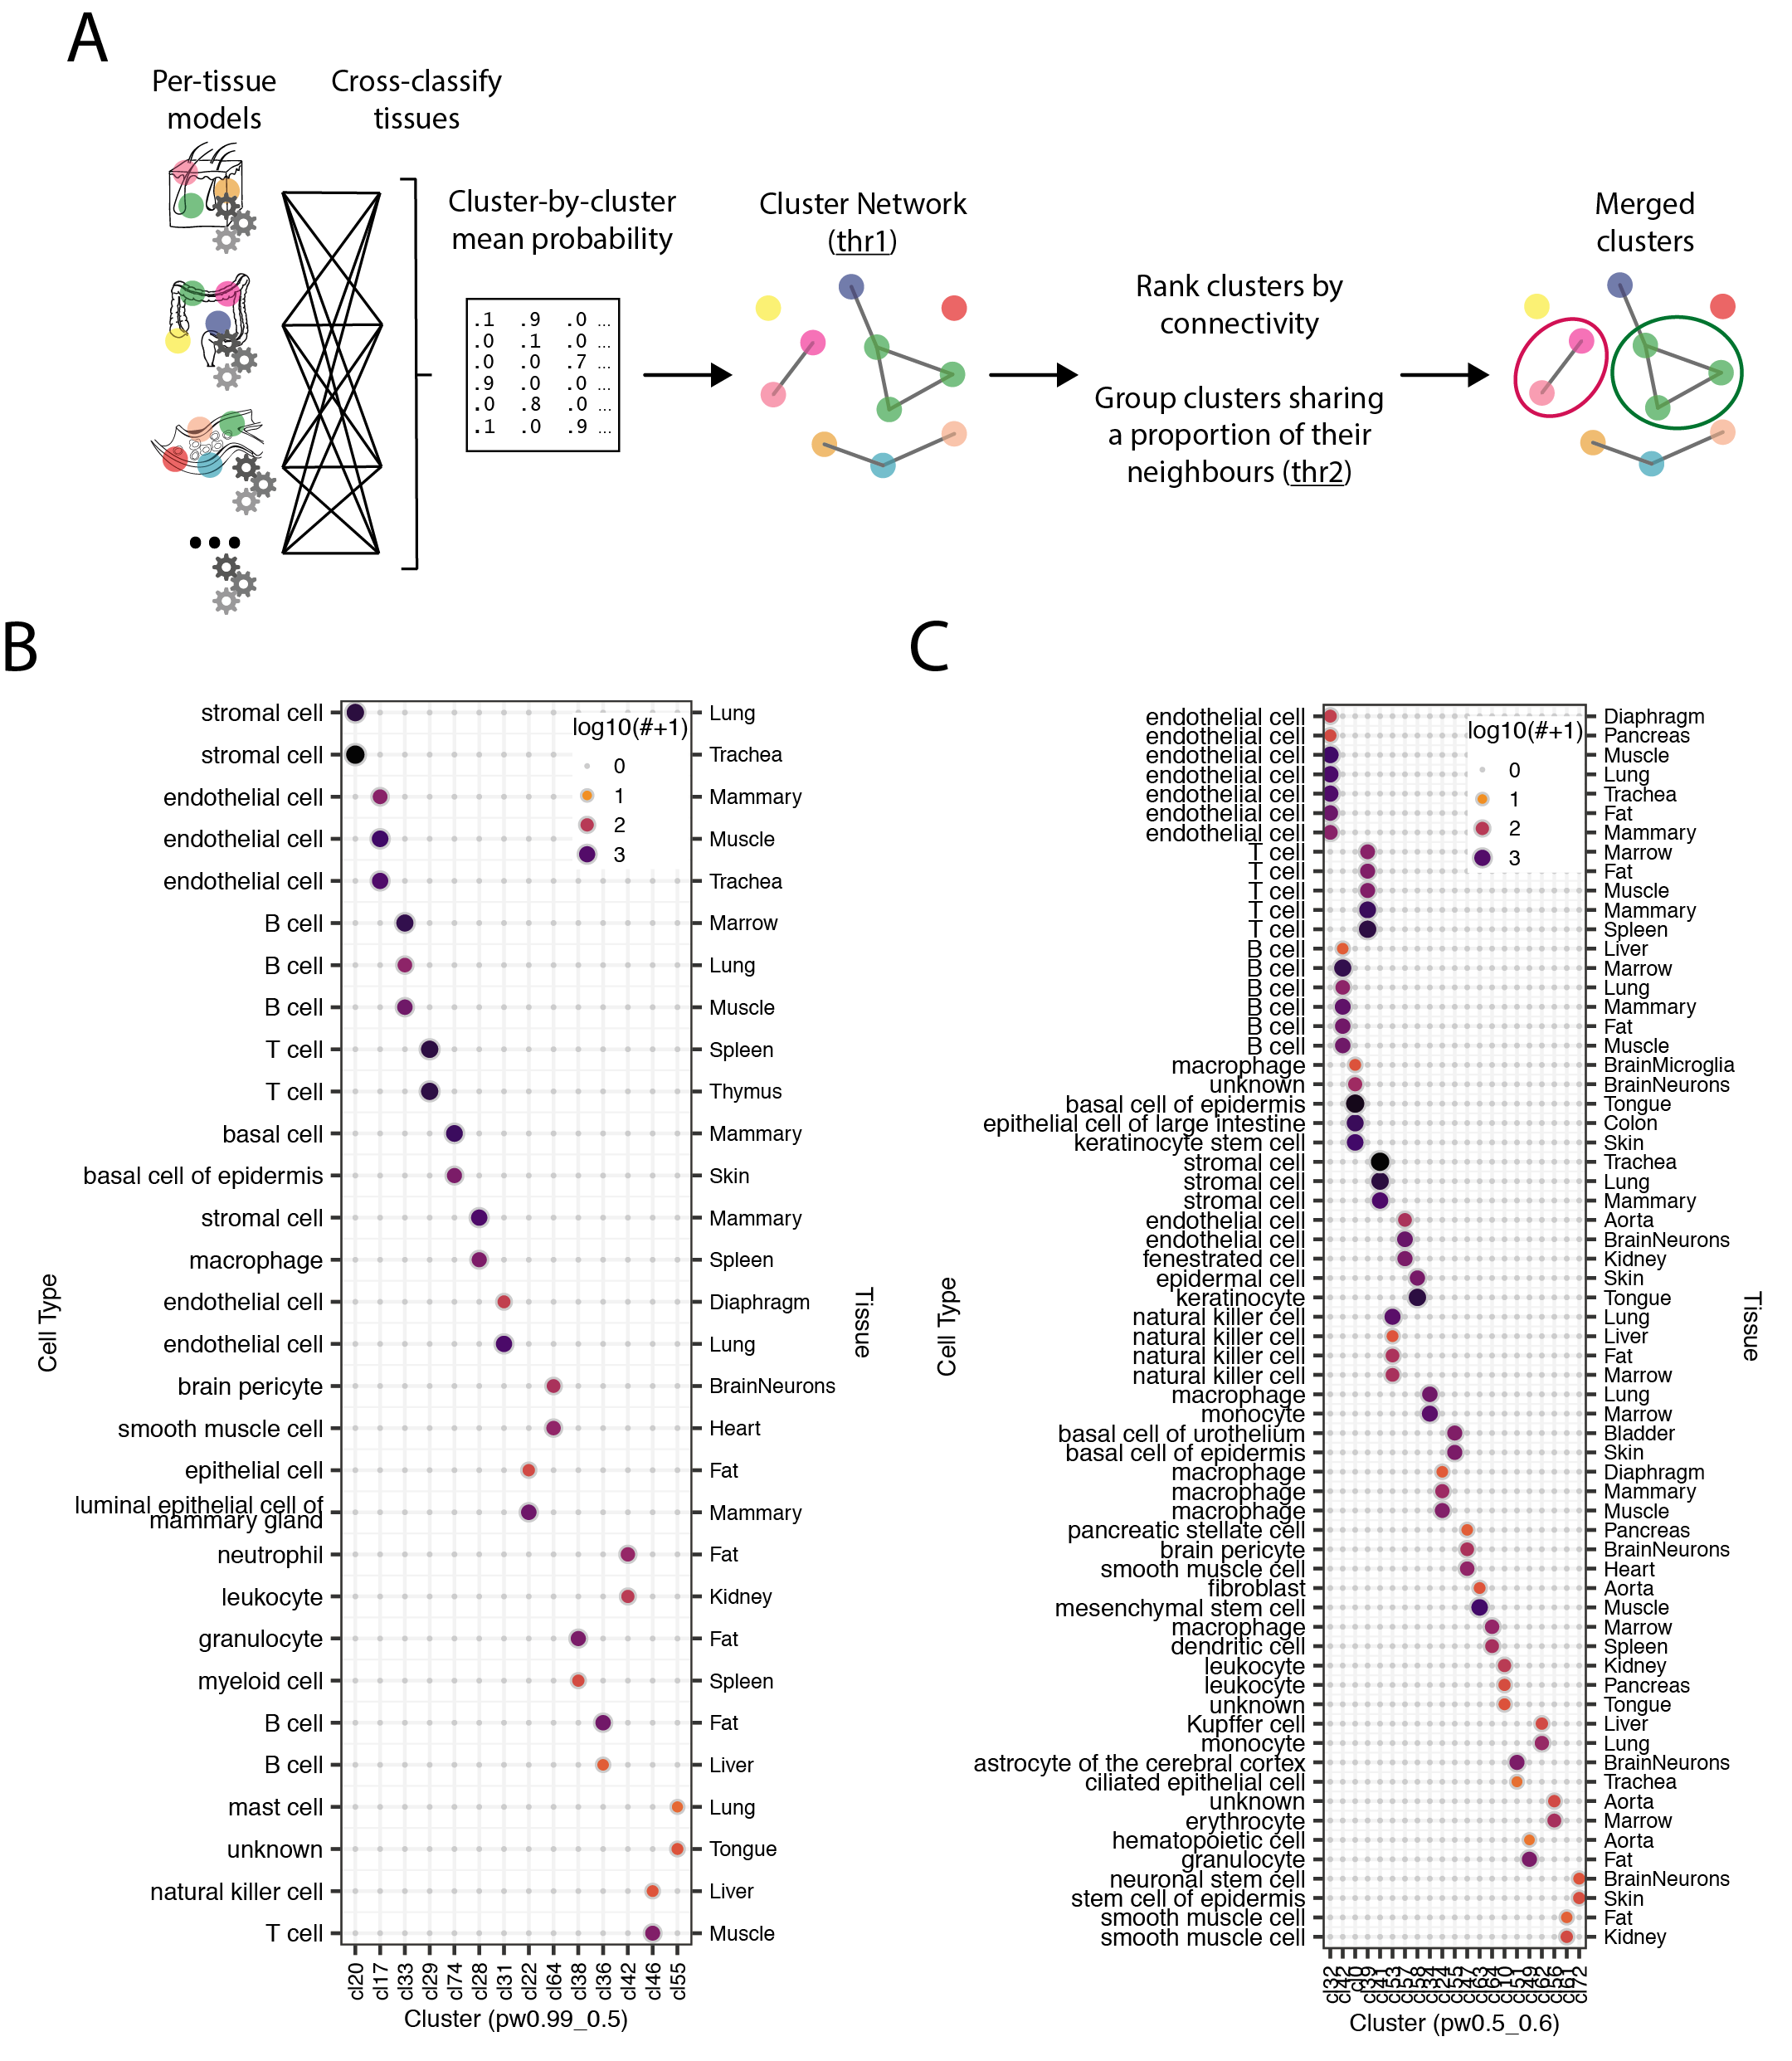
\includegraphics[width=1.0\textwidth]{Chapter3/Figs/chap3_combineClusters.png} % change word in curlies to change figure
    \caption[Cross-tissue matching of cell types]{\textbf{Cross-tissue matching of cell types}\newline\textbf{(A)} For each tissue, a logistic regression model is trained, and used obtain a classification probability of all tissues. Clusters are then linked depending on the mean probabilities of one cluster matching another (\textit{thr1}). Clusters are ranked on connectivity, and grouped with neighbouring clusters that share a proportion of its neighbours (\textit{thr2}). (Continued on the following page.)}
    \label{fig:chap3_combcl}
\end{figure}
\begin{figure}[t]
  \contcaption{(continued) \textbf{(B and C)} Merging of cell types (x-axis) using the method in (A) for models trained on known cell type labels (left y-axis). \textbf{(B)} shows the top parameter combination (thr1 = 0.99, thr2 = 0.5) based on split-join distance; \textbf{(C)} shows the combination that came in third (thr1 = 0.5, thr2 = 0.6) and which resulted in increased merging.}% Continued caption
\end{figure}

% B and C - testing using the cell types as labels - what cell types get merged?
To test how this algorithm performed in a situation with known labels, it was tested using the annotated cell types for each tissue instead of clusters. After ranking the solutions given by the different parameter combinations tested (combinations identical to Figure~\ref{fig:chap3_combdat}B), we inspected the top parameter combination (Figure~\ref{fig:chap3_combcl}B, thr1 = 0.99 and thr2 = 0.5), as well as the third, which presented the lowest combined cluster number (Figure~\ref{fig:chap3_combcl}C, thr1 = 0.5 and thr2 = 0.6). Most clusters resulting from the merging workflow, in both solutions, combined cell types annotated with the same name in different tissues. This is particularly evident for endothelial cells, B cells, and T cells. While the score for the merging  presented in panel C was not as good as that for panel B, it is immediately apparent that the more extensive merging still conserves most of the correct labeling, even grouping together identical cell types that are left separate in the first solution. This indicates that there can be a range of approximately correct parameter combinations, and hints at the tissue specificity of certain widespread cell types. Taking as an example endothelial cells, the first combination leaves lung and diaphragm separate from the remaining tissues.

% how it looks with clusters
This merging was then performed on the tissue clusters obtained in the first section of the pipeline. Both thresholds in the algorithm were tested with the values 0, 0.1, 0.2, 0.25, 0.3, 0.4, 0.5, 0.6, 0.7, 0.75, 0.8, 0.9, and 0.99. With the increase of both parameters, we observe an increase in the total number of clusters and a decrease in the fraction of merged clusters (Figure~\ref{fig:chap3_combdat}A). This trend is more evident for thr2, which is more directly involved in determining which clusters are kept together. Parameter combinations were then ranked based on their reduction of the split-join distance when comparing with known cell type labels, taking the original per-tissue clusters as a baseline. The parameter grid (Figure~\ref{fig:chap3_combdat}B) shows lower values for this ratio at higher thr2 values, with the top combination at thr1 = 0.8, thr2 = 0.99. Examining this combination for how cell type labels were grouped revealed that, similarly, to Figure~\ref{fig:chap3_combcl}B and C, many similar cell types had been grouped together (e.g. T cells; endothelial cells). Moreover, we can observe that cells with different names but similar functions are grouped together, as is the case of endothelial cells and fenestrated cells (an endothelial cell part of the renal glomerulus). In contrast, however, it could be observed that some cell types dispersed across more than one cluster. Even so, in cases where this happened (e.g. kidney tubule cell; mesenchymal stem cell of adipose), this dispersion tended to be minor, with a majority of cells from each of these annotated cell types coalescing in one cluster.

In sum, this demonstrates that this workflow is capable of merging cells with a similar transcriptome, and making cell identity across tissues uniform.


\subsection{Model training and evaluation}
\label{section3.2.3}

\begin{figure}[ht!] % LAST FIGURE FROM NEXT SECTION (PLACED HERE FOR FORMATING)
    \centering    
    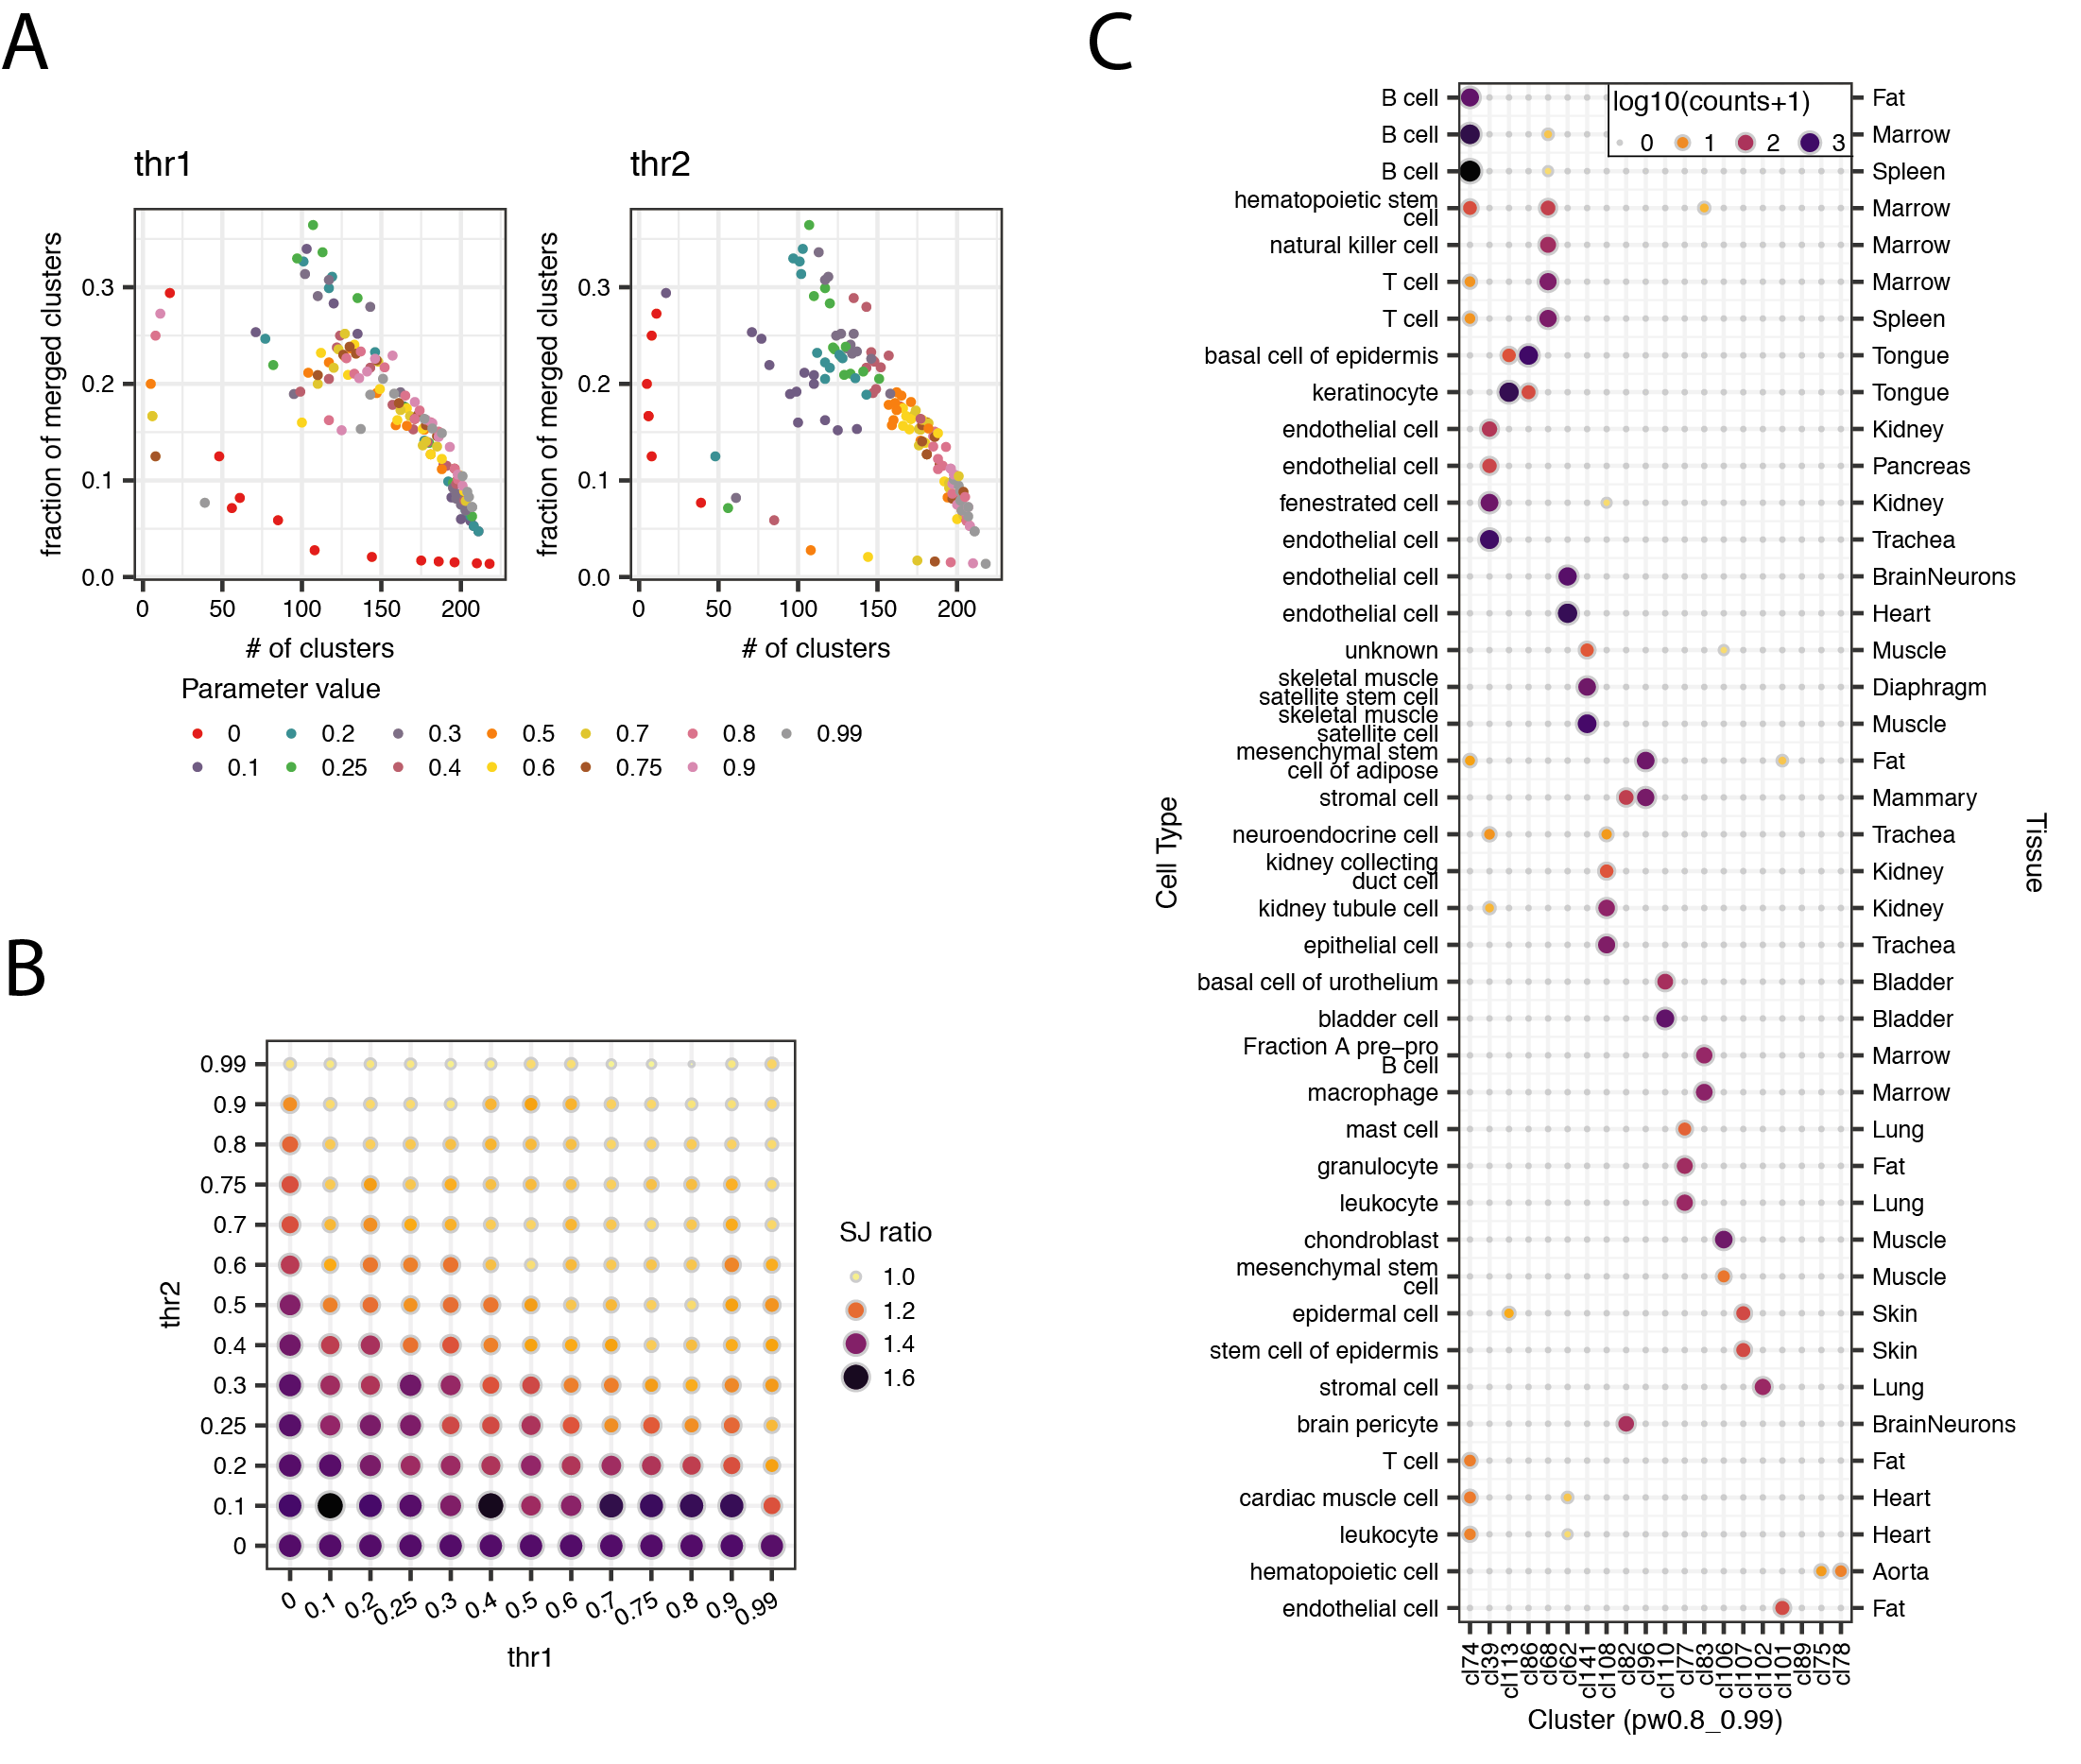
\includegraphics[width=1.0\textwidth]{Chapter3/Figs/chap3_combineData.png} % change word in curlies to change figure
    \caption[Evaluation of clusters matched across tissues]{\textbf{Evaluation of clusters matched across tissues}\newline\textbf{(A)} Change in number of total clusters and fraction of merged clusters with each threshold value (see Figure~\ref{fig:chap3_combcl}A for reference). Parameters resulting in a single cluster were not represented. \textbf{(B)} Parameter grid showing the variation of the ratio of split-join distance between merged clusters and cell type annotation, and per-tissue clusters and cell type annotation. \textbf{(C)} Grouping of cell types contained in per-tissue clusters (x-axis) using the top parameter combination (thr1 = 0.8, thr2 = 0.99) based on split-join distance.}
    \label{fig:chap3_combdat}
\end{figure}

\begin{figure}[ht!]
    \centering
    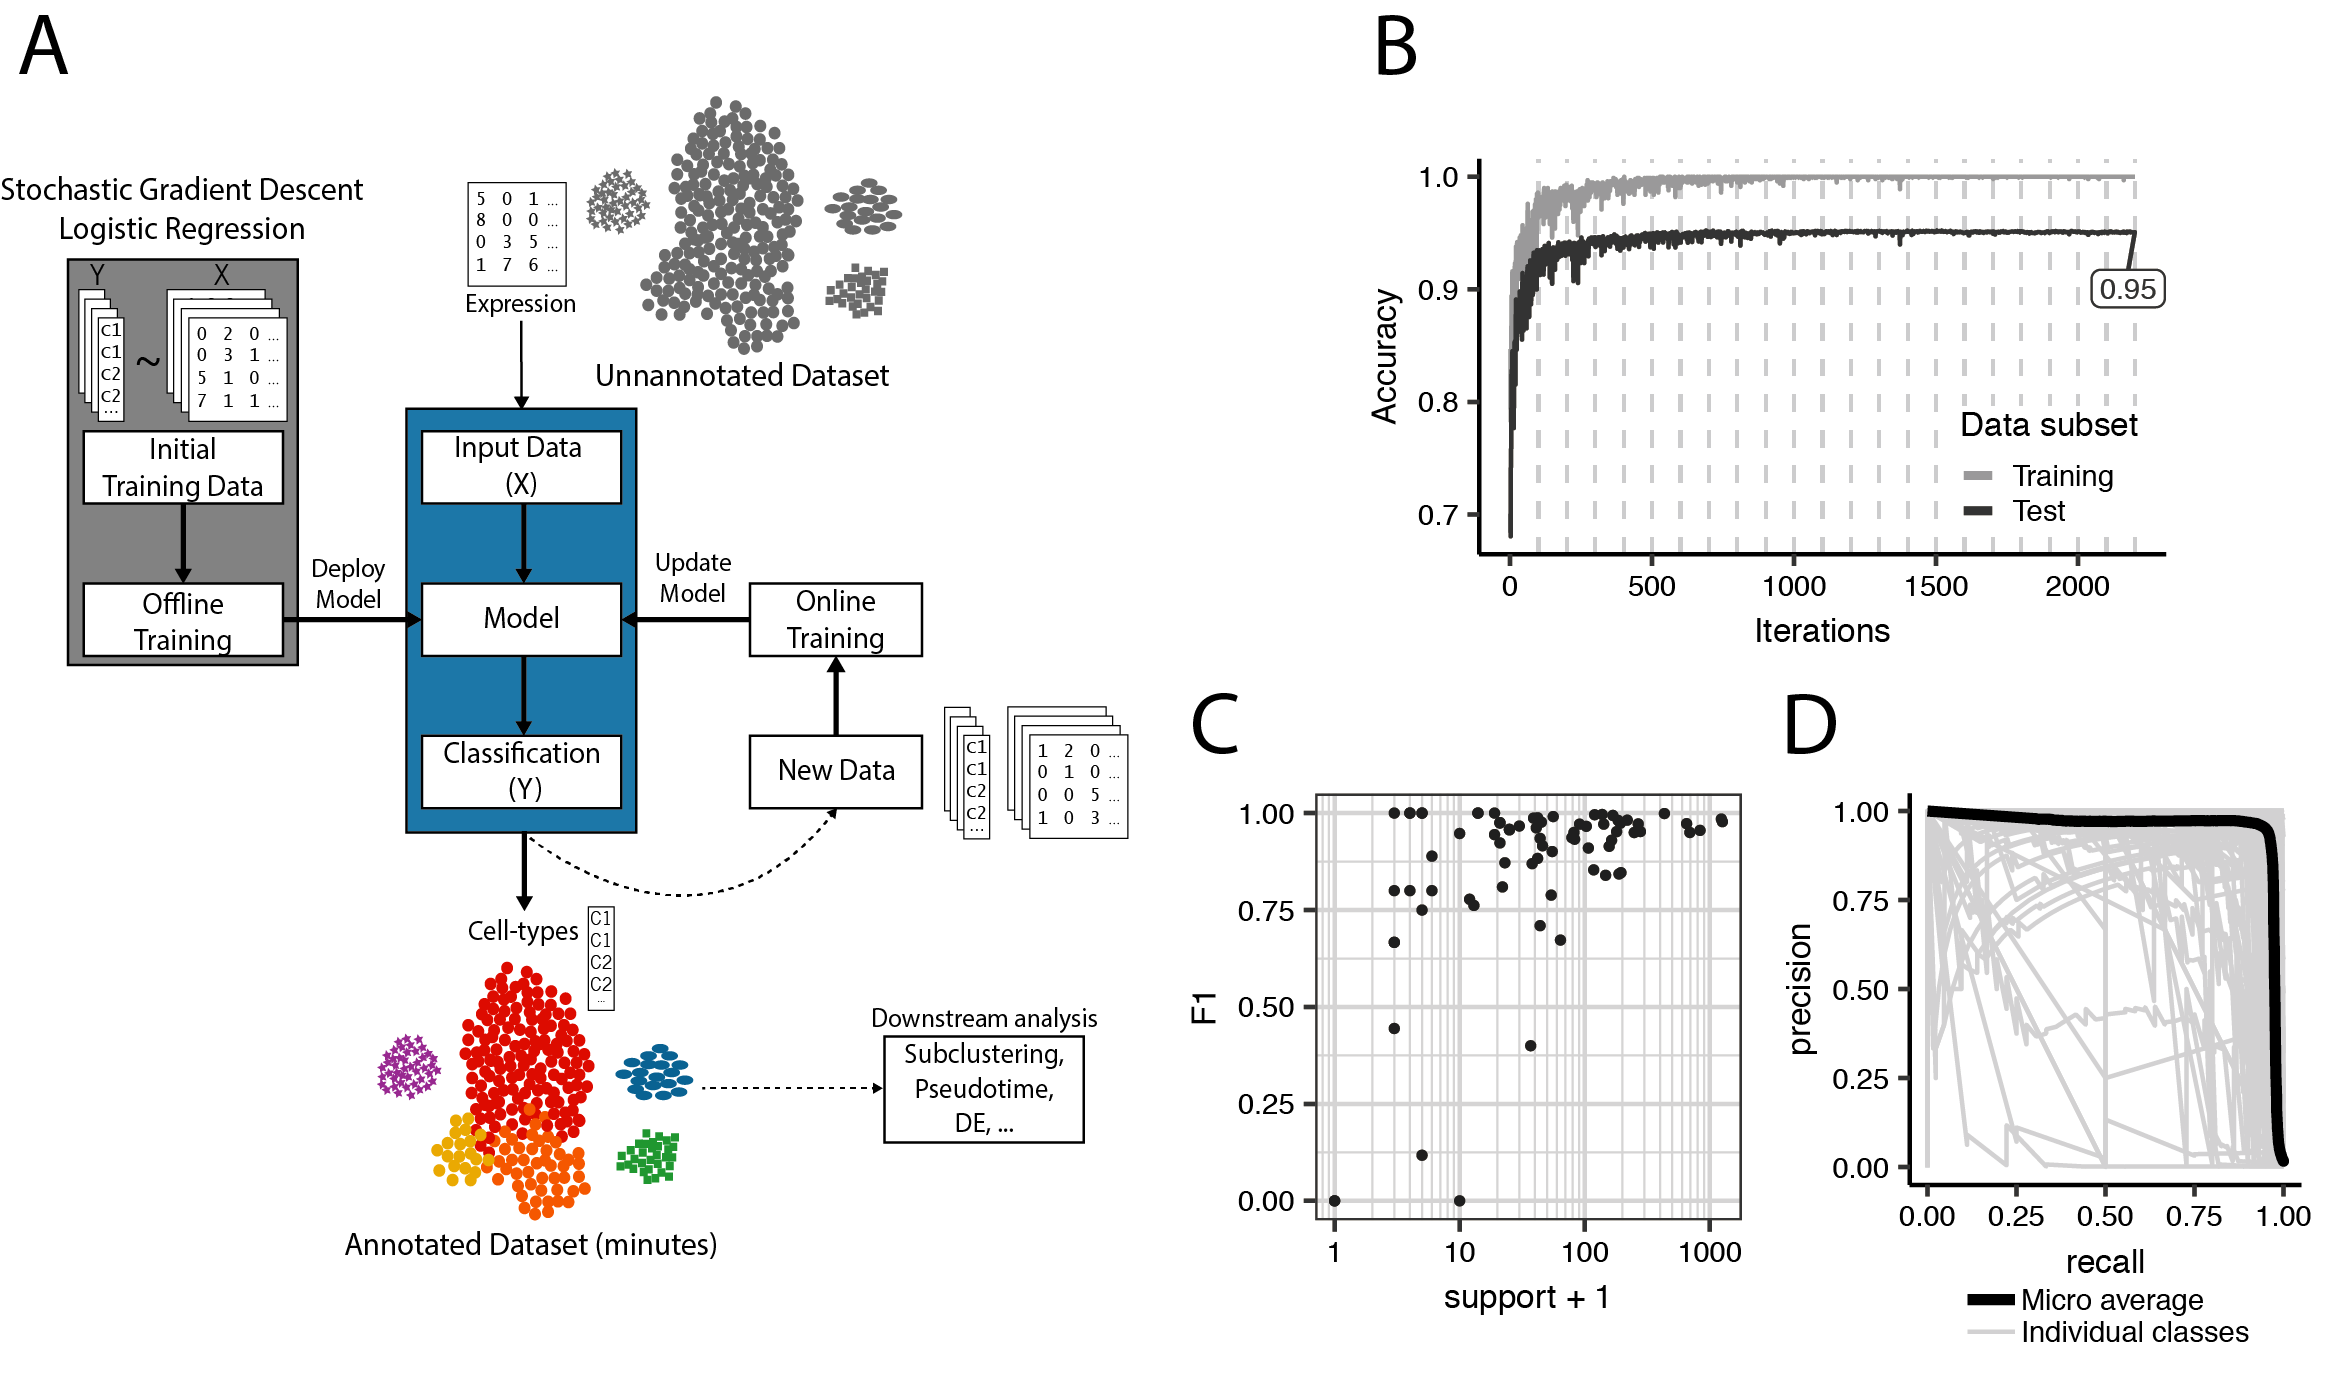
\includegraphics[width=1.0\textwidth]{Chapter3/Figs/chap3_model.png} % change word in curlies to change figure
    \caption[Model training outline and evaluation]{\textbf{Model training outline and evaluation}\newline\textbf{(A)} Model training and usage outline. A logistic regression model is trained using stochastic gradient descent. When deployed, it can provide annotations for unlabelled data, which can the be further supplied back into the model to update it. \textbf{(B)} Accuracy during model fitting for training and held-out test data, to directly predict \textit{Tabula Muris} cell type labels. Vertical dashed lines represent each training epoch. Terminal label indicated final accuracy for prediction in the test set. \textbf{(C)} F1-score for each cell type (black dots) as a function of class size (in log10 scale). \textbf{(D)} Precision-curves for each cell type (gray), and global micro average (black).}
    \label{fig:chap3_model}
\end{figure}

% explain models, mention how the per-tissue and global models were trained
The last step in \textit{CellTypist} is training the classifier. The goal of the classifier is to provide a fast and unbiased cell identity annotation of new datasets (Figure~\ref{fig:chap3_model}A). \textit{CellTypist}'s classifier is implemented in Python using scikit-learn~\citep{scikit-learn}, and uses a logistic regression model with L2 regularization. This allows the model to remain accurate, while still providing information about the contribution of all genes to determining the classification of each cell type. Training is done through mini-batch training using stochastic gradient descent (SGD). SGD is used since it makes the model more scalable, as it can converge without training over the whole dataset, needing approximately one million data points, provided that all observations from all labels are passed to it. For the models here presented however, the model will see the whole data a fixed number of times (epochs), to present its behaviour during training. The model encompassing all tissues was trained for 25 epochs, and the models trained on individual tissues (used in~\ref{section3.2.2}, Figure~\ref{fig:chap3_combcl}) were trained for 10 epochs. Additionally, SGD also allows for online training, meaning that if new data is obtained it can be easily incorporated into the model.

\begin{figure}[ht!]
    \centering    
    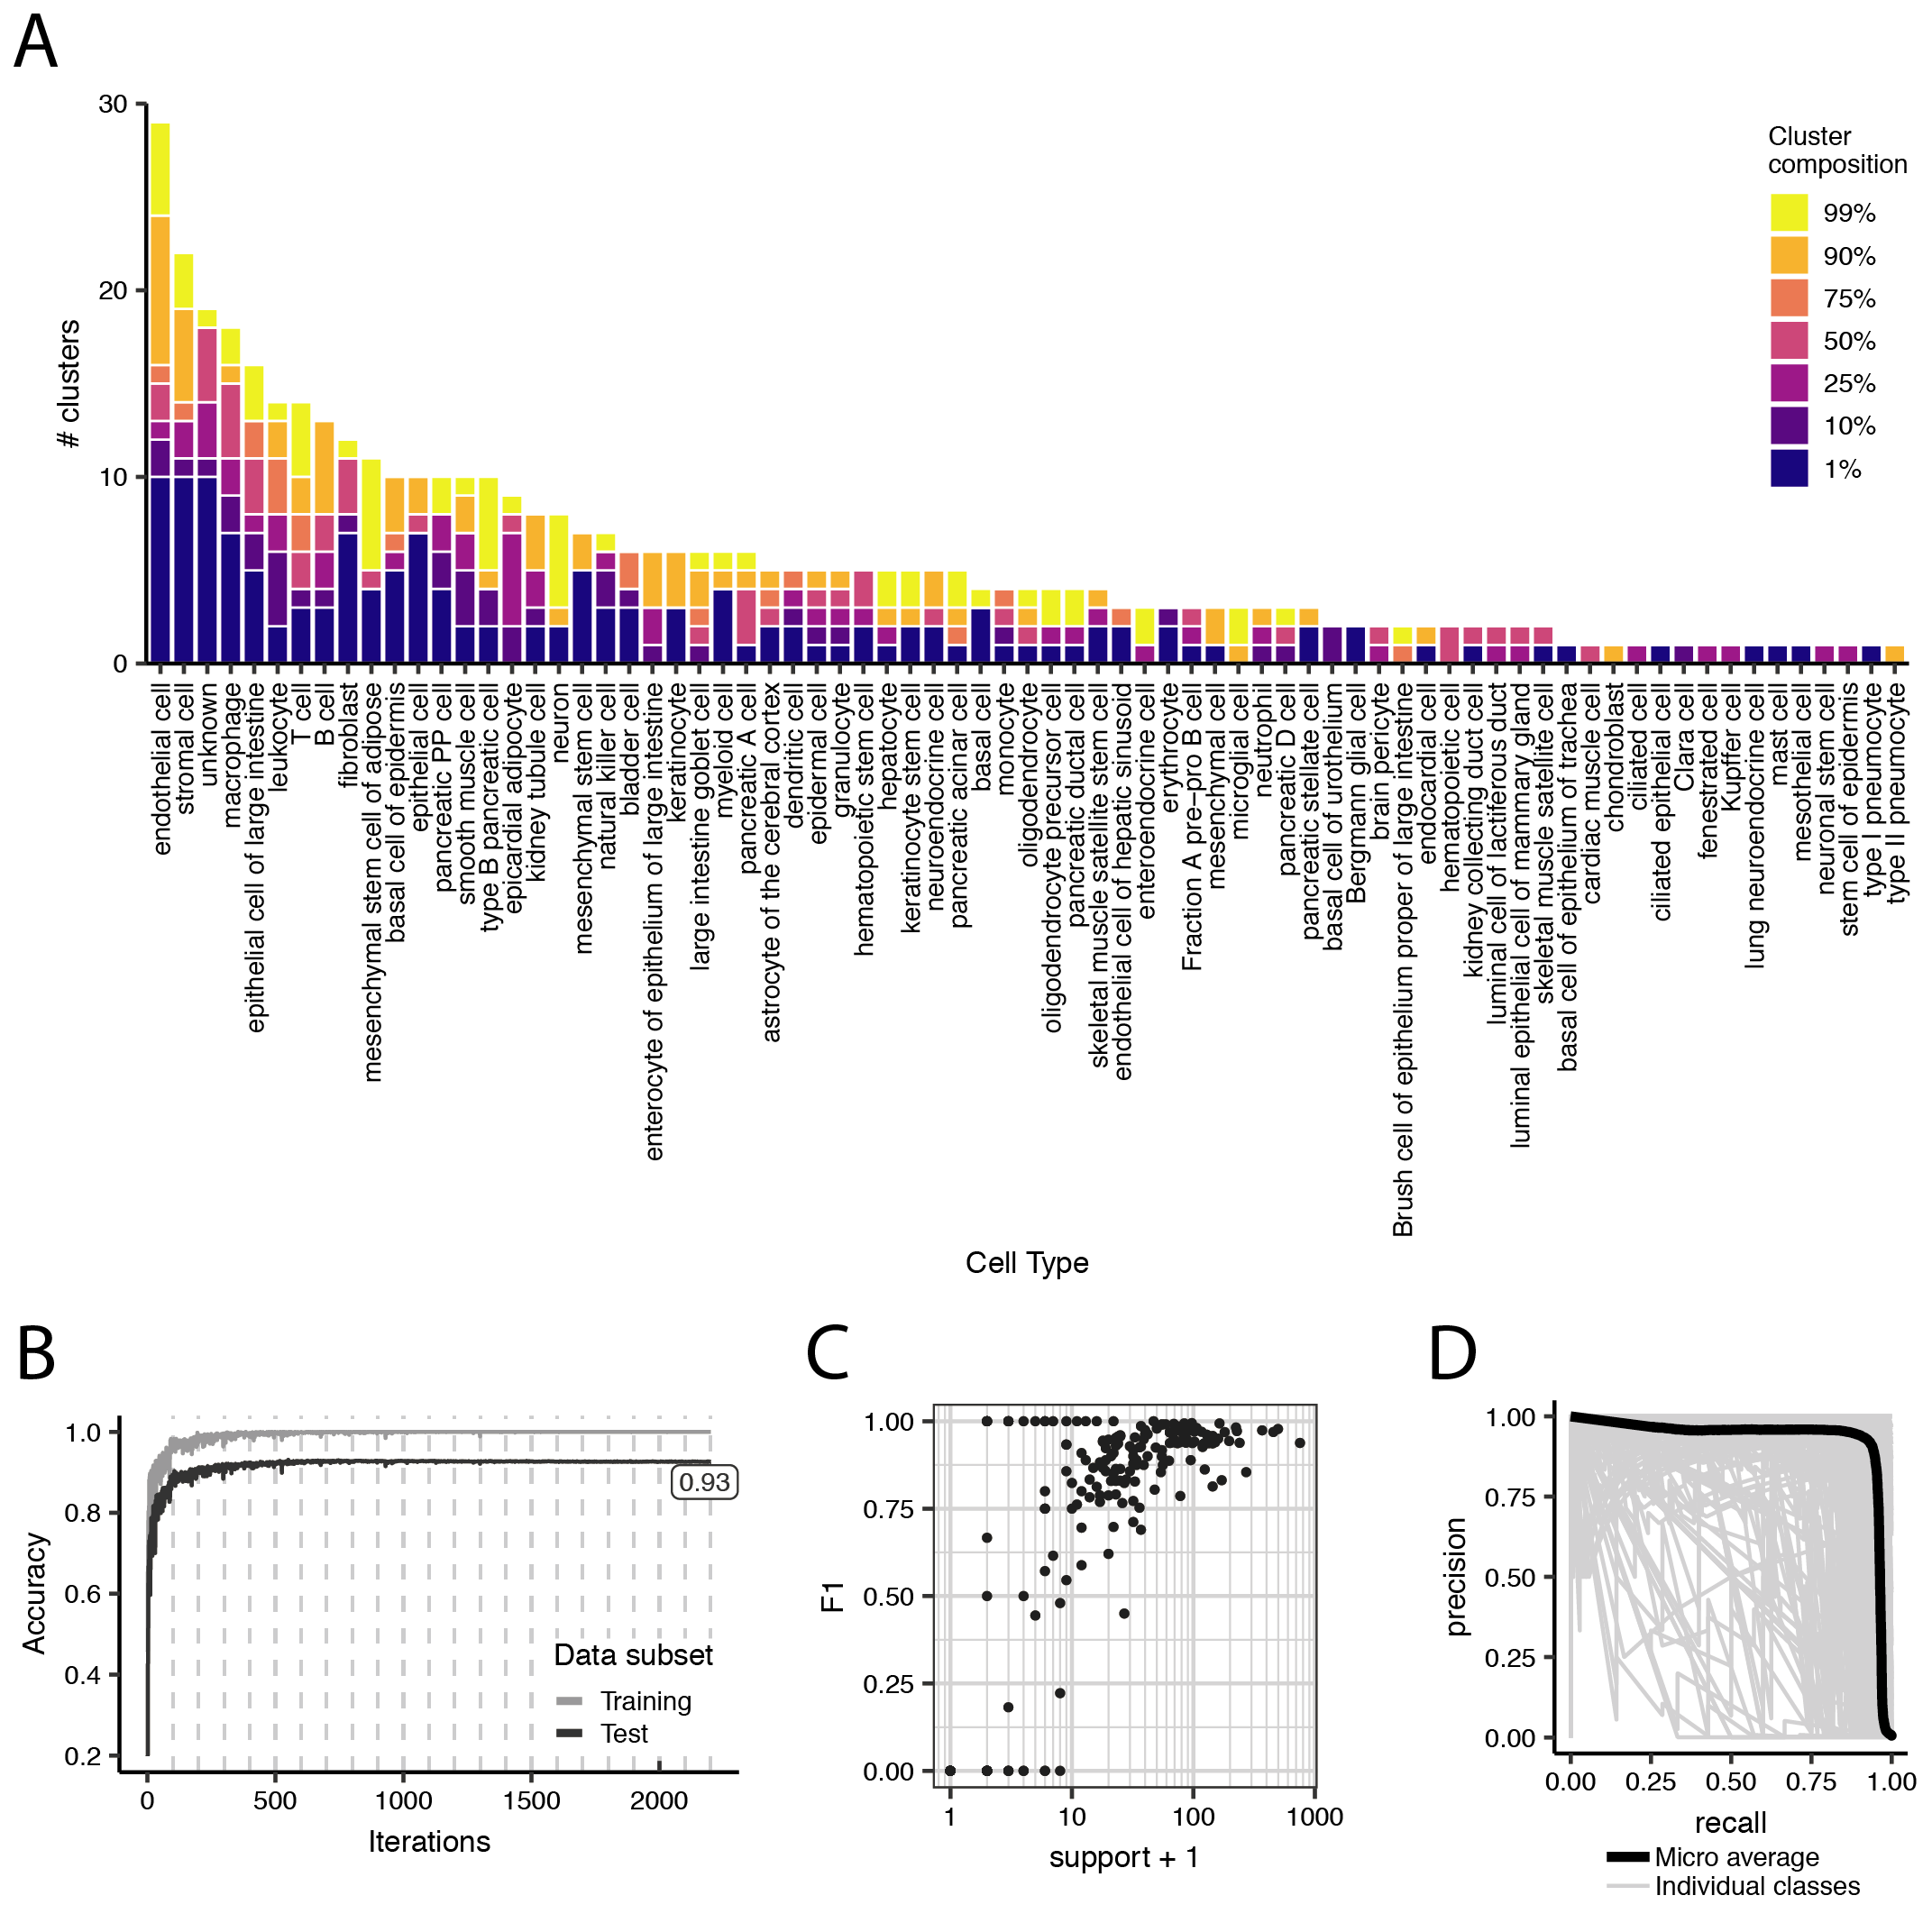
\includegraphics[width=1.0\textwidth]{Chapter3/Figs/chap3_modelcl.png} % change word in curlies to change figure
    \caption[Evaluating model trained on cross-tissue integrated clusters]{\textbf{Evaluating model trained on cross-tissue integrated clusters}\newline\textbf{(A)} Abundance of annotated cell types in cross-tissue clusters. Colours represent clusters with at least x\% of a given cell type. \textbf{(B)} Accuracy during model fitting for training and held-out test data, to predict cross-tissue integrated clusters. Vertical dashed lines represent each training epoch. Terminal label indicated final accuracy for prediction in the test set. \textbf{(C)} F1-score for each cluster label (black dots) as a function of class size (in log10 scale). \textbf{(D)} Precision-curves for each cluster (gray), and global micro average (black).}
    \label{fig:chap3_modelcl}
\end{figure}

This methodology was tested on the complete \textit{Tabula Muris} dataset, training the model to predict the existing cell type annotations. The model converged after fewer than 500 iterations (each iteration corresponding to a batch of 1000 cells), and resulted in a prediction accuracy of 95\% on the held-out test set (Figure~\ref{fig:chap3_model}B). Performance per class was assessed by calculating the F1 score, i.e. the harmonic mean between precision and recall for each class. A partial dependency between this score and the number of cells in a give class was observed for smaller groups (fewer than 100 cells, Figure~\ref{fig:chap3_model}C). The strong predictive capability of the model can be further observed by plotting the precision-recall curves for each class (Figure~\ref{fig:chap3_model}D). While we again observe some classes to have a poorer performance, a micro-averaging of precision and recall of all classes (i.e. average precision and recall by calculating true positives, false positives and false negatives for each class) shows a very strong performance.

The model training framework was further tested using the cluster labels resulting from the merging shown in Figure~\ref{fig:chap3_combdat} (thr1 = 0.8, thr2 = 0.99). Figure~\ref{fig:chap3_modelcl}A examines the representation of annotated cell types across all clusters, showing that a large majority of cell types are in one or more clusters where they represent at least 90\% of cells. Similarly to the cell type-based model, performance metrics globally show a fast convergence and high training accuracy (Figure~\ref{fig:chap3_modelcl}B), as well as a high per-label precision and recall (Figure~\ref{fig:chap3_modelcl}C, D), with most classes having an F1 score above 0.75.

These results demonstrate the high performance of simple and intuitive logistic regression to train models capable of annotating data from various sources.


\nomenclature[z-SGD]{SGD}{Stochastic Gradient Descent}

\section{Discussion}
\label{section3.5}
\textit{CellTypist} has been designed as a way of systematising cell identity from expression data, and use it directly for automatic annotation. The pipeline has been designed keeping scalability in mind, fully aware that the first model represents an initial release that will be continuously updated. It is expected that the increase in data sources and available expert annotations will greatly improve the usability of the framework going forwards.

The construction of the \textit{CellTypist} pipeline is also subject to evolution. It has been developed with the ability to include unannotated data in a cell type reference. Existing cell type annotation is highly informative when deposited together with the expression data or the accompanying publication, although this is not always the case. Even so, the vast majority of scRNA-seq analysis pipelines rely either on Leiden~\citep{traag_louvain_2019} or Louvain~\citep{blondel_fast_2008} clustering, which are used in the per-tissue processing step and thus results in a considerable approximation between known and new labels (Figure~\ref{fig:chap3_pertiss}B). Even though the final, merged labels can be manually curated and named, existing cell type annotations can also be made available to the end user, adding another layer of validation to the results.

The results here presented demonstrate that integration using the pipeline correctly merges similar cell types (Figures~\ref{fig:chap3_combcl}B,C and~\ref{fig:chap3_combdat}C). However, these results are not perfect. Figure~\ref{fig:chap3_combdat}C shows that the merged clusters are composed of more than one annotated cell type, and can at times include cells with unrelated annotations. This unexpected mixing is not a result of the cluster matching procedure, but rather a product of the initial per-tissue clustering step (Figure~\ref{fig:chap3_pertiss}C). The initial step combining datasets is thus crucial to obtain clusters representing specific cell types with high purity, while retaining as much cell type/state specificity as possible. The fact that, in some instances, T cells share clusters with natural killer cells, is an example that the method does not yet achieve perfect cell type separation. These two cell types have similar transcriptomes, which explains why in some reduced representations used for clustering they might appear very close. Nonetheless they are easily distinguishable by the expression of a small set of markers, and can thus be efficiently distinguished by a logistic regression model (Figure~\ref{fig:chap3_model}C and D). 

The resolution bottleneck introduced by the first, per-tissue integration step can be potentially improved in a few ways. One possibility is to adopt a more curated approach after clustering every tissue, although this would require significantly more human input. Another option would be to rely more on data with existing annotations. One way to achieve this is by using a label propagation method that, within each integrated tissue, passes existing labels to unannotated data~\citep{barkas_joint_2019}. Alternatively, the method can instead iteratively apply the algorithm used to integrate the clusters between tissues (Figure~\ref{fig:chap3_combcl}A). In the first step this would be applied for each dataset collected to merge all existing data for each tissue, and relying on existing annotations. A second step would then be applied between tissues as shown (Figure~\ref{fig:chap3_combcl}). This guarantees that any known heterogeneity in the collected data is preserved and propagated into the final annotation, but has the disadvantage that any novel populations that would be detected by data integration can be lost.

This Chapter also demonstrated the viability of logistic regression as a methodology for cell type classification using a broad atlas as a reference (Figures~\ref{fig:chap3_model}B-D and~\ref{fig:chap3_modelcl}B-D). This is in line with previous reports~\citep{kohler_deep_2019,abdelaal_comparison_2019}, showing that cell identity classification is not improved by the use of deep learning methods, and can be accurately performed using simpler machine learning frameworks. The results here also demonstrate that this method is robust enough to accommodate clusters with some mixture of cell types (which results in lower phenotypic resolution) (Figure~\ref{fig:chap3_modelcl}C).

The implementation of \textit{CellTypist} is also explicitly constructed such that the resulting model can be easily updated. This is due to the implementation using stochastic gradient descent, which allows for easy and direct updates to the model by running more learning iterations on novel data. This is important to maintain the reference up to date. However, it can only be done by classifying new data according to the existing labels. If the new datasets collected include cell types that are not represented in \textit{CellTypist}, then the full pipeline needs to be ran anew. Nonetheless, this allows for the database to have fast minor releases to maintain it up to date with the latest dataset publications, as well as less frequent major releases that more thoroughly integrate these datasets and revise the annotation database. \textit{CellTypist} will be available with a web interface, allowing for classifications to be ran via a web server, or, alternatively, download the models to test locally. It will include a database characterising the cell type labels present in the model. While different organisms will have different models, many of the cell types described are predicted to be present in multiple species, and can in future updates have their cross-species similarities defined and reflected in \textit{CellTypist}'s accompanying cell type compendium.

% usefulness (will be demonstrated in the next chapter)
Overall, this chapter has demonstrated that \textit{CellTypist} can organise a valuable resource for cell type annotation. Furthermore, this resource can be readily interpreted from inspection of gene coefficients for each label. In the next chapter, a practical application and interpretation of \textit{CellTypist} using human data will be presented.
%!TEX root = ../thesis.tex
%*******************************************************************************
%****************************** Fourth Chapter *********************************
%*******************************************************************************
\chapter{Application and biological insights of the \textit{CellTypist} model} \label{chap:CT_test}

% **************************** Define Graphics Path **************************
\ifpdf
    \graphicspath{{Chapter4/Figs/Raster/}{Chapter4/Figs/PDF/}{Chapter4/Figs/}}
\else
    \graphicspath{{Chapter4/Figs/Vector/}{Chapter4/Figs/}}
\fi
The identity of a cell can be defined by the genes it expresses. A continuously increasing number of studies has applied scRNA-seq to profile cells from various body locations and describe the cells that make up a tissue, in the steady-state or disease. A smaller number of studies have focused on the differences between the cell types detected in different tissues~\citep{miragaia_single-cell_2019,scott_transcription_2018}. However, we don't yet know how variable the transcriptome of most cell types is between tissues, and how much of a tissue's transcriptomic identity is reflected in each cell type.

This Chapter outlines the construction of a human cell type reference based on single-cell transcriptomics, by applying the \textit{CellTypist} framework presented in Chapter~\ref{chap:CT_method}. The present Chapter will focus on the interpretability of this pipeline, and reveal the genes driving cell identity across tissues. We will further dissect the relationships across tissues established by \textit{CellTypist}, and explore the influence of different major cell types in tissue biology.

The analyses here performed are based on the methodology outlined in Chapter~\ref{chap:CT_method}. Supplementary figures and tables are included in Appendix~\ref{appendix:CTsub}.


\section{Introduction}
\label{section4.1}
Recent developments in single-cell sequencing have enabled unbiased and high-throughput assessment of cell types through transcriptomic profiling~\citep{svensson_exponential_2018}. A few individual works have aimed at profiling cell types across most tissues of an organism~\citep{fincher_cell_2018,plass_cell_2018,han_mapping_2018,noauthor_single-cell_2018}. Other more complex and detailed cellular census have been done for individual tissues, and large consortia have been established to aggregate some of these datasets and establish guidelines and collaborations to identify all cell types across an organism~\citep{regev_human_2017}.




% defining and cataloguing cell types
The definition of cell type is, like many biological terms, a working definition. Cells have been classified based on different aspects of their morphology, molecular phenotype, or function. Historically, this knowledge of cell identity has been restricted to specific fields (e.g. immunology, neuroscience), hindering the development  of an integrative, systemic perspective of cell types in the body. Single-cell RNA-seq technologies (scRNA-seq) are now challenging this perspective, since they allow for an unbiased profiling of cell identity through the transcriptome. As scRNA-seq data acquisition grows~\citep{svensson_exponential_2018}, so does our understanding of the cellular make up of the profiled tissues. The Human Cell Atlas Consortium has defined as one of its goals to develop a cellular taxonomy~\citep{regev_human_2017}, which is necessarily harmonised across tissues. Nonetheless, a unified, transcriptome-driven perspective of cell identity is still lacking.

% understanding tissue and cell function
The molecular basis for the relationships between tissues were initially probed by high-throughput methods; first microarrays~\citep{enard_intra-_2002}, and later with RNA-seq~\citep{mortazavi_mapping_2008,brawand_evolution_2011,barbosa-morais_evolutionary_2012}. More recent studies are now linking this transcriptome cross-tissue  variability with genome variants~\citep{consortium_genotype-tissue_2015,gtex_consortium_genetic_2017}, unravelling the regulatory determinants behind tissue biology. Further analysis have delved into the importance of transcription factors for tissue identity~\citep{sonawane_understanding_2017}, revealing that tissue specificity lies not only in these molecules but mostly on the tissue-specific regulatory roles they play, while also showing that transcription factors are less likely to be identified as tissue-specific than other genes. An integrated predictive model of cell identity should be able to reveal patterns relating tissues through cell identity relationships, as well as offer a broad perspective of the genes determining cell types.

% this chapter
Here we will expand on the \textit{CellTypist} pipeline previously defined, and how it can be used to probe cellular identity in human primary cells across body locations. We detail the collection and integration of various human datasets, totalling close to 1.5 million cells from 21 different tissues. After applying \textit{CellTypist}, its integrated results are examined for cross-tissue relationships. The pipeline can recapitulate known tissue associations, caused either by comparable cell sampling (e.g. tissues solely profiled for immune cells), or by functional similarity. These are evident both at the tissue integration stage, as well as in the top genes learned by the model that define cell groupings in each tissue. These genes are further examined for patterns in cell identity definition, revealing a global pattern for genes coding for functional effector molecules (i.e. receptors and secreted proteins) to be more pivotal in defining cell identity than others involved in genomic regulation. Finally, we discuss the potential uses and implementation of a scRNA-seq-derived cell type reference.


\section{Results}
\label{section4.2}
\subsection{Human data collection and organisation}
\label{section4.2_coll}
To obtain a global, cross-tissue perspective of human cell types, we obtained a broad representation of single-cell transcriptomes by collecting several publicly available scRNA-seq datasets (Table~\ref{table:tab_4_1}). Information about tissue, scRNA-seq protocol, sampling method, and cell type annotation (when available) were obtained from the respective publications and data repositories, together with the gene expression matrices.

% table: Dataset; number of cells; ref
\begin{table}[ht!] % p for putting it in the next page available
\footnotesize
\caption[Datasets collected and references]{Datasets collected and references}
\centering
\label{table:tab_4_1}

\begin{tabular}{l|c|r}
\toprule
~\textbf{Dataset} & ~\textbf{Reference} & ~\textbf{\# cells} \\
\midrule
baron16 & ~\citep{baron_single-cell_2016} & 8.569  \\

bjorklund16 & ~\citep{bjorklund_heterogeneity_2016} & 648  \\

gierahn17 & ~\citep{gierahn_seq-well:_2017} & 3.694  \\

guo18 & ~\citep{guo_adult_2018} & 12.053  \\

habib17 & ~\citep{habib_massively_2017} & 14.963  \\

hcaImmune18 & \href{data.humancellatlas.org}{HCA Data Portal} & 593.844  \\

henry18 & ~\citep{henry_cellular_2018} & 109.061  \\

jaitin19 & ~\citep{jaitin_lipid-associated_2019} & 13.199  \\

james20 & \textit{Unpublished} & 32.228  \\

lamanno16 & ~\citep{la_manno_molecular_2016} & 1.977  \\

li19 & ~\citep{li_memory_2019} & 1.886  \\

masuda19 & ~\citep{masuda_spatial_2019} & 6.144  \\

menon18 & ~\citep{menon_single-cell_2018} & 9.846  \\

miragaia18 & ~\citep{miragaia_single-cell_2019} & 1.168  \\

muraro16 & ~\citep{muraro_single-cell_2016} & 2.126  \\

nowakowski17 & ~\citep{nowakowski_spatiotemporal_2017} & 4.261  \\

popescu19 & ~\citep{popescu_decoding_2019} & 113.063  \\

segal19 & ~\citep{segal_single_2019} & 1.475  \\

segerstolpe16 & ~\citep{segerstolpe_single-cell_2016} & 3.363  \\

smillie19 & ~\citep{smillie_intra-_2019} & 110.110  \\

sohni19 & ~\citep{sohni_neonatal_2019} & 34.729  \\

takeda19 & ~\citep{takeda_single-cell_2019} & 33.257  \\

vento18 & ~\citep{vento-tormo_single-cell_2018} & 69.883  \\

vieira19 & ~\citep{braga_cellular_2019} & 26.013  \\

wang16 & ~\citep{wang_single-cell_2016} & 635  \\

young18 & ~\citep{young_single-cell_2018} & 44.526  \\

zhang18 & ~\citep{zhang_lineage_2018} & 5.989  \\

zheng17 & ~\citep{zheng_massively_2017} & 163.234  \\
\midrule
\textbf{\textit{Total}} &  & 1.421.944  \\

\bottomrule
\end{tabular}
\end{table}

\begin{figure}[ht!]
    \centering    
    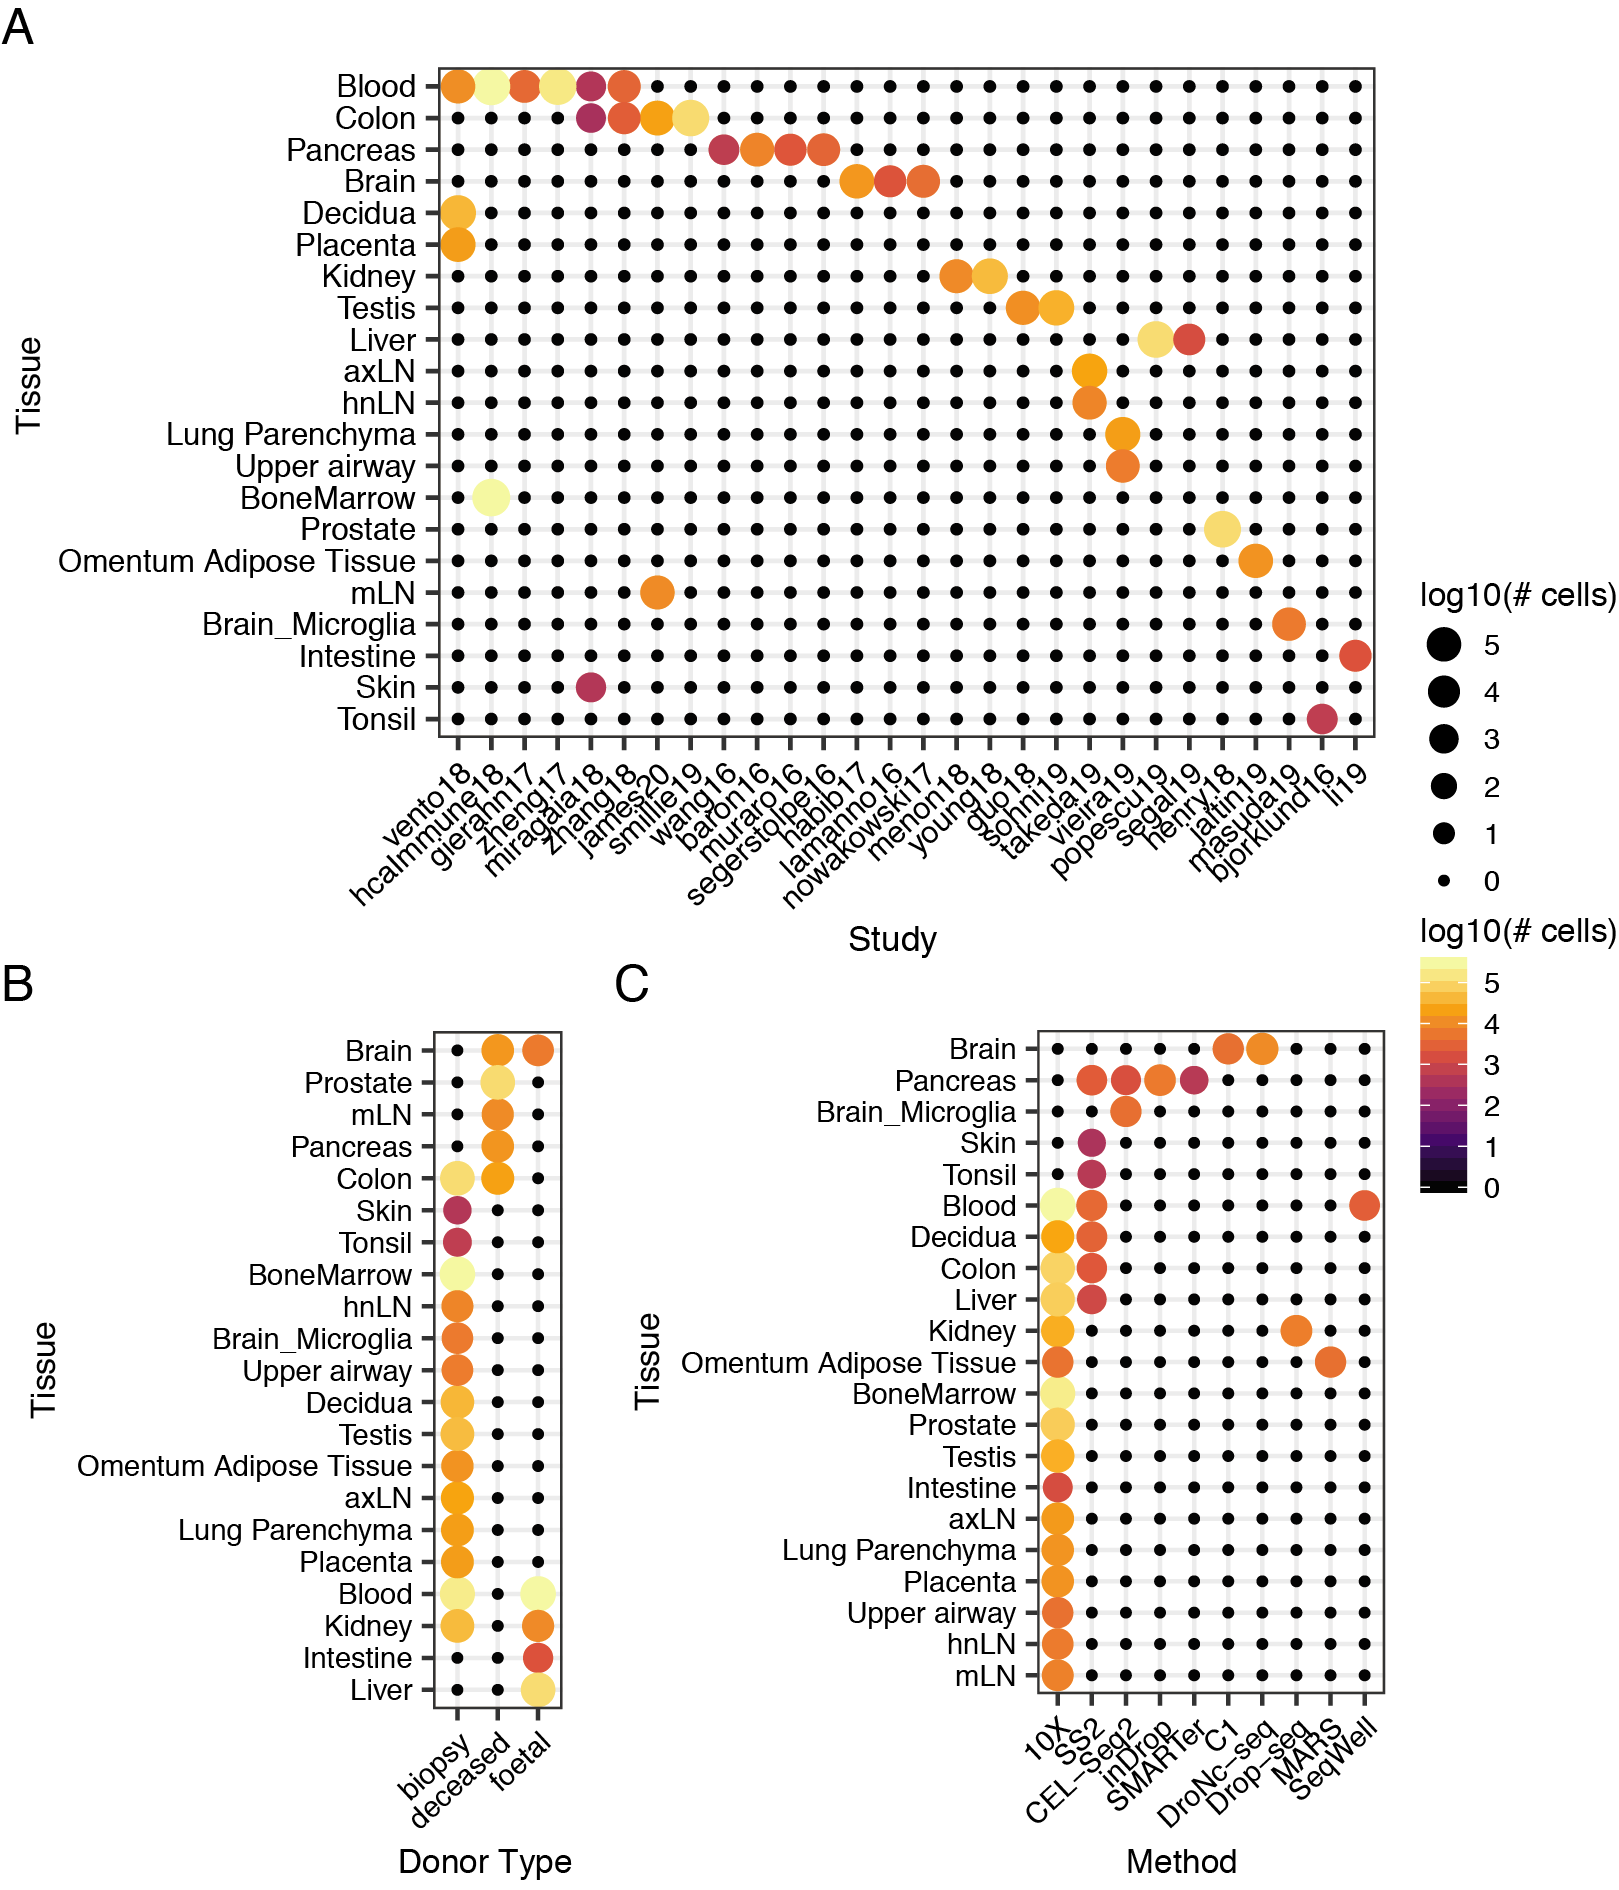
\includegraphics[width=1.0\textwidth]{Chapter4/Figs/chap4_countsHumanAtlas.png} % change word in curlies to change figure
    \caption[Cell numbers in the human dataset collection]{\textbf{Cell numbers in the human dataset collection} \newline Number of cells, in log10 scale, collected from different tissues, and distributed by publication \textbf{(A)}, type of collection \textbf{(B)}, and scRNA-seq protocol \textbf{(C)}. hnLN - head and neck lymph nodes; axLN - axilary lymph nodes; mLN - mesenteric lymph nodes.}
    \label{fig:chap4_cha}
\end{figure}

The 28 datasets collected include 21 tissues, mostly collected from adult biopsies (Figure~\ref{fig:chap4_cha}A and ~\ref{fig:chap4_cha}B), and totalling close to 1.5 million cells. Various studies focus on haematopoietic-derived cells, and as such many of the sampled tissues are mostly composed of immune cells (Figure~\ref{fig:appB_ptprc}). Most cells are obtained using the droplet-based "Chromium" instrument from 10x Genomics ("10X" in Figure~\ref{fig:chap4_cha}C), followed by the plate-based, full-length Smart-seq2 ("SS2"). Despite this unbalance in usage of different technologies, it is in agreement with what has been reported in an exhaustive curated reference of single-cell sequencing datasets~\citep{svensson_curated_2019}.

The collected expression matrices for the listed datasets were combined, and gene references were matched across all datasets (Methods Section~\ref{section4.4_datacol}). This was done to maintain the integrity of each dataset, as well as facilitate data collection and incorporation (see Section~\ref{section4.3}). The \textit{CellTypist} pipeline was then applied to this collection (see Methods Section~\ref{section4.4_model}), and parameter optimisation was done as described in the previous chapter, first selecting for each tissue a clustering resolution that yielded the lowest split-join distance between clusters and available cell type annotations (Figure~\ref{fig:chap4_HA}A), and then choosing the set of merged clusters that most resemble the existing cell type annotations in each dataset (Figure~\ref{fig:chap4_HA}B). Applying the optimised parameter combination (thr1 = 0.99, thr2 = 0.8, see Figure~\ref{fig:chap3_combcl}A) resulted in 627 clusters (Figure~\ref{fig:appB_grids}A). An example of a tissue (pancreas) with consistently annotated cell types across datasets can be seen in Figure~\ref{fig:appB_panc}. Using these clusters, a model was then trained as previously shown (Figure~\ref{fig:chap3_model}A, Methods Section~\ref{section4.4_model}) with a classification accuracy of 84\% on left-out test data (Figure~\ref{fig:chap4_HA}C). The F1 statistic calculated for each label was in most cases above 0.75, meaning elevated precision and recall in the model, especially for clusters with more than 100 cells, as previously shown (Figure~\ref{fig:chap3_model}C, Figure~\ref{fig:chap3_modelcl}C).

\begin{figure}[ht!]
    \centering    
    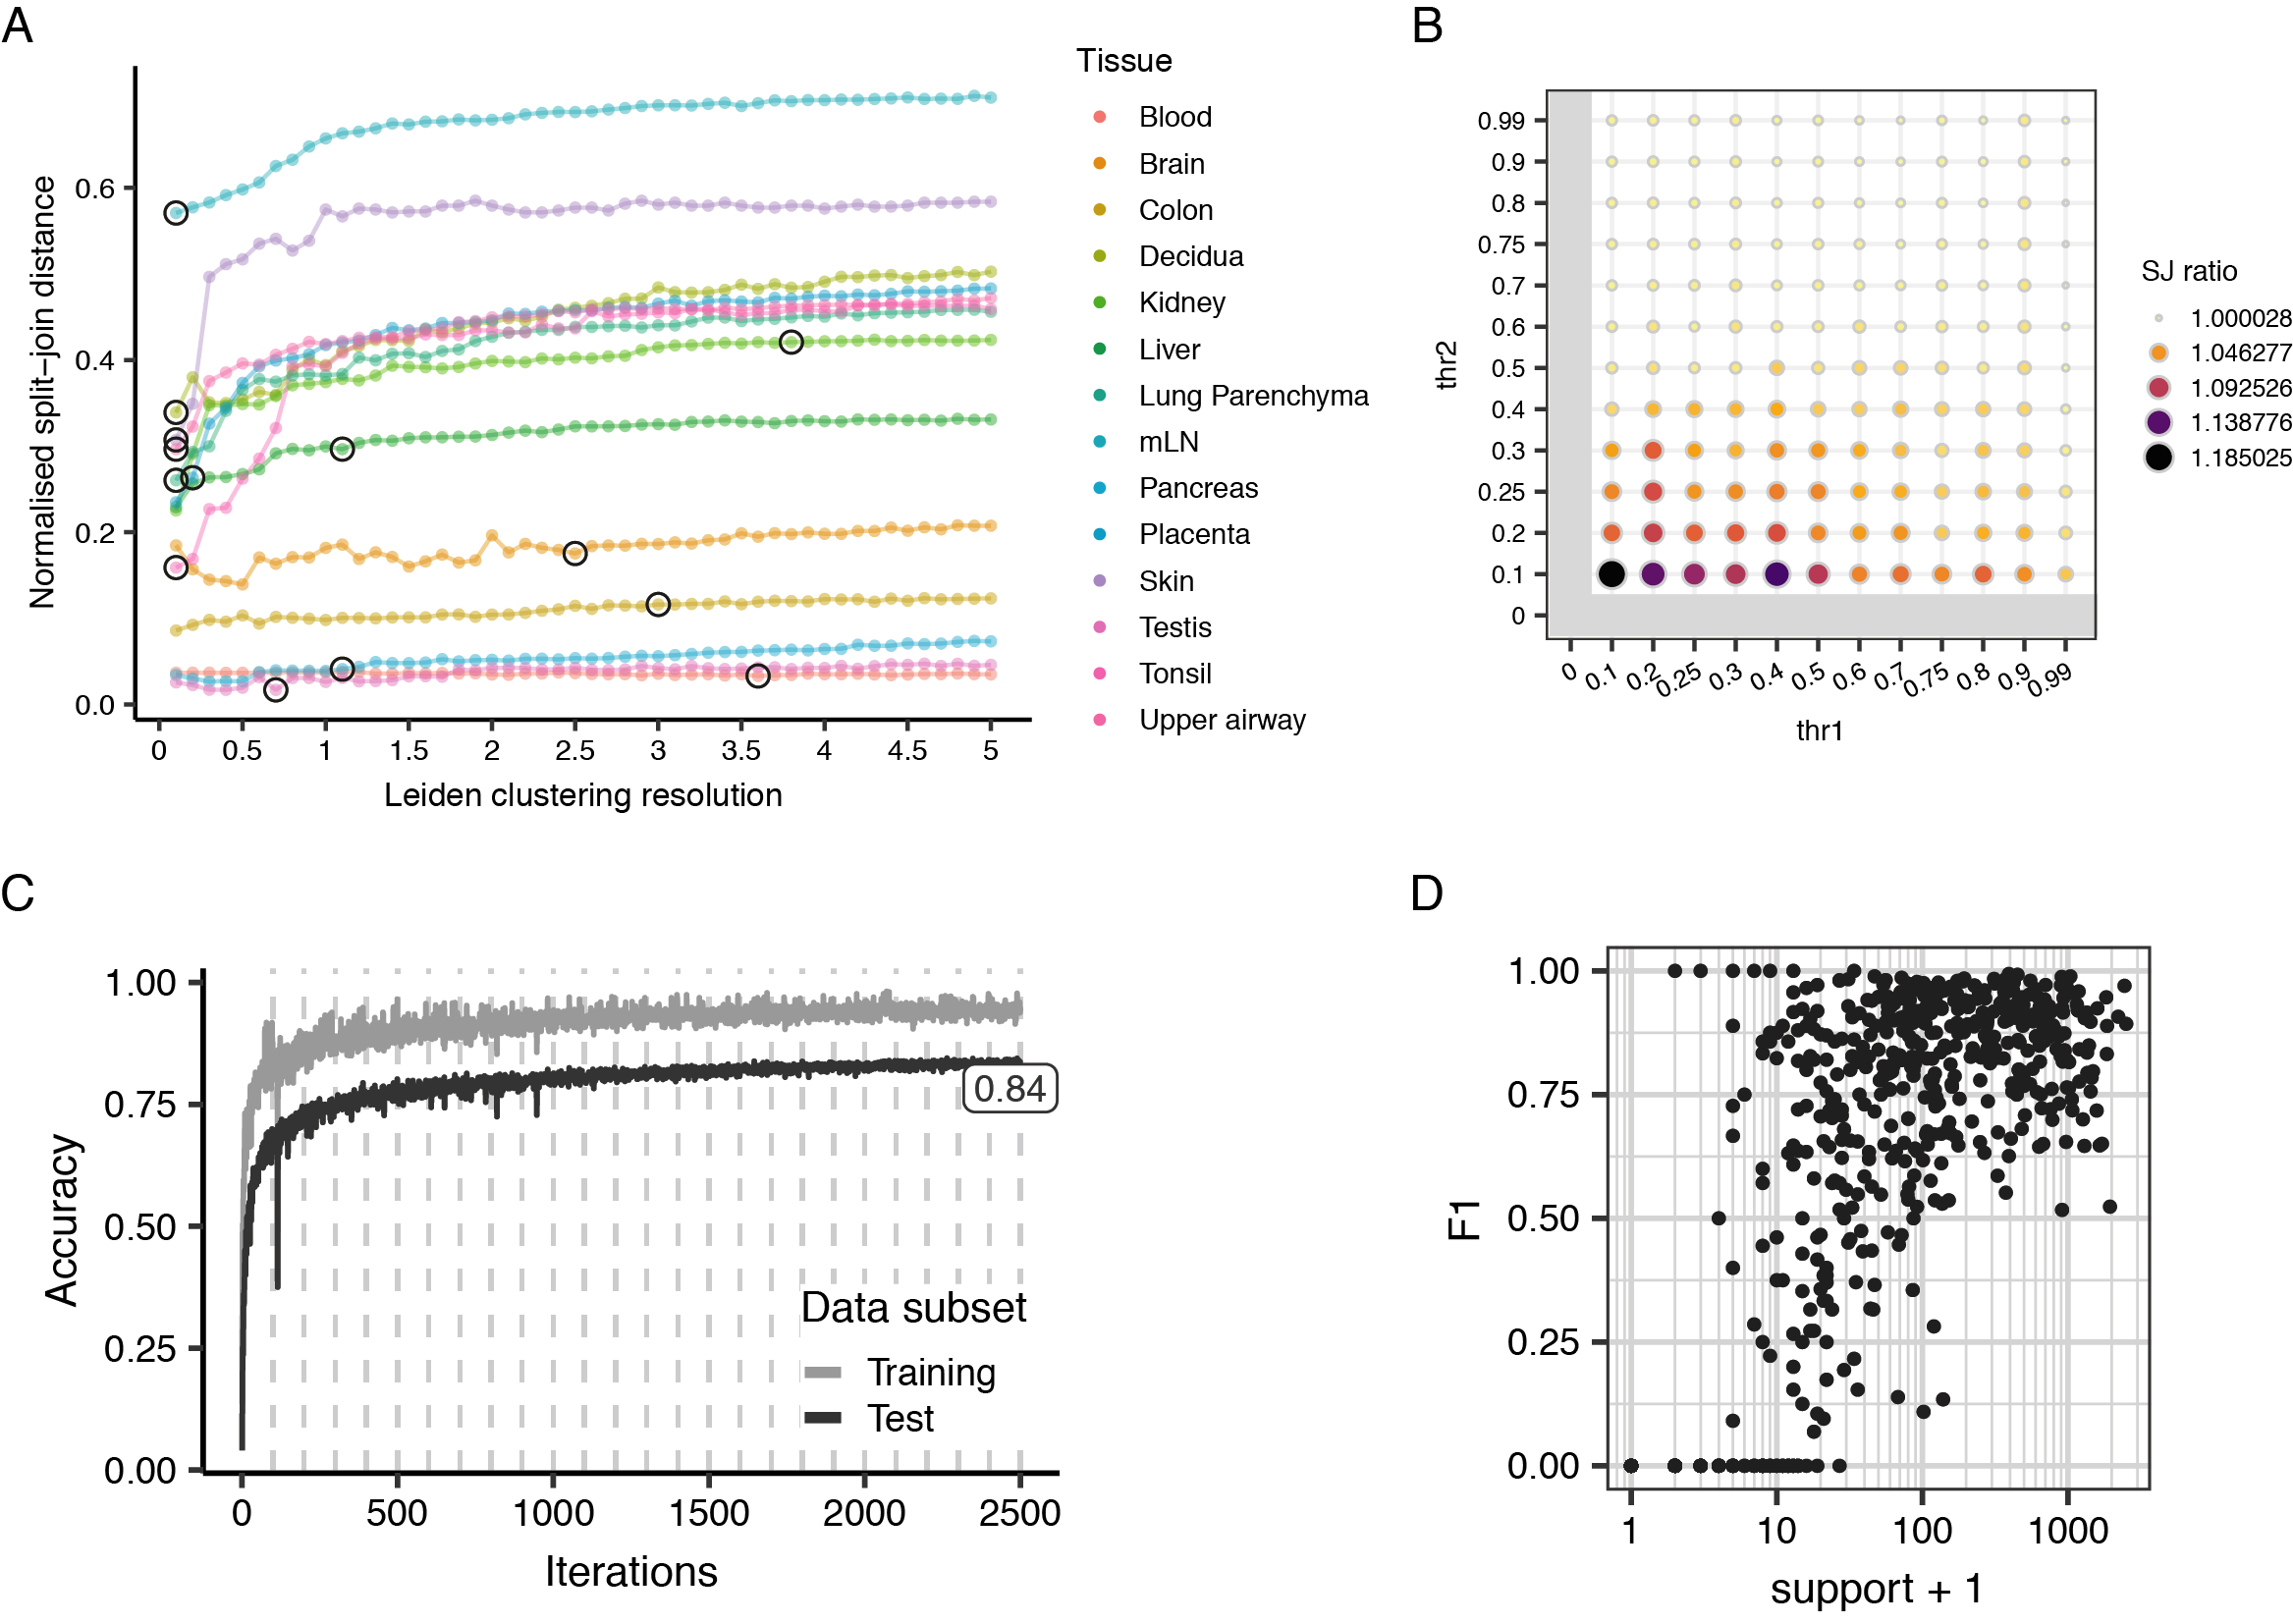
\includegraphics[width=1.0\textwidth]{Chapter4/Figs/chap4_figHA.png} % change word in curlies to change figure
    \caption[Running \textit{CellTypist} on a human scRNA-seq data collection]{\textbf{Running \textit{CellTypist} on a human scRNA-seq data collection}\newline\textbf{(A)} Per-tissue cluster optimisation, choosing the resolution that approximates existing cell type annotations. Similarity is measured with normalised split-join distance, and constrained to solutions with a number of clusters of at least as many as existing annotations in the largest collected dataset. Selected values are indicated with a black circle. \textbf{(B)} Grid of parameters tested for cross-tissue cluster merging, showing the variation of the ratio of split-join distance between merged clusters and cell type annotation, and per-tissue clusters and cell type annotation (colour and size of points). \textbf{(C)} Accuracy during model fitting for training and held-out test data, to predict cross-tissue integrated clusters obtained using thr1 = 0.99 and thr2 = 0.8 as parameters for \textit{CellTypist} (optimal value in (B)). Vertical dashed lines represent each training epoch. Terminal label indicated final accuracy for prediction in the test set. \textbf{(D)} F1-score for each cluster label (black dots) as a function of class size (in log10 scale).}
    \label{fig:chap4_HA}
\end{figure}

Three additional models, trained using sets of clusters derived using different parameters, were also examined. These were thr1 = 0.4 and thr2 = 0.99 (Figure~\ref{fig:appB_moremodels}A-B), thr1 = 0.25 and thr2 = 0.25 (Figure~\ref{fig:appB_moremodels}C-D), and thr1 = 0.1 and thr2 = 0.1 (Figure~\ref{fig:appB_moremodels}E-F, see Methods Section~\ref{section4.4_model}). These models show a lower performance, in particular the latter (thr1 = 0.1 and thr2 = 0.1), with a test classification accuracy of 73\%. This may be due to the excessive merging of clusters within and across tissues, thus leading to hybrid, undetermined groups of cells (Figure~\ref{fig:appC_tissrel}). Other models are more conservative in this regard, and show a better classification performance. The model using clusters obtained with thr1 = 0.25 and thr2 = 0.25 still has noticeably worse values for the split-join distance, yet also represents a more condensed cell type reference (420 clusters), without sacrificing accuracy (83\%). Lastly, the model with the parameters thr1 = 0.4 and thr2 = 0.99, in particular, is the one showing the greatest improvement in matching annotated cell types after cross-tissue merging, and is thus another possible reference model.

In sum, the collected datasets allow for the training of the \textit{CellTypist} pipeline and construct a fully interpretable human cell type reference.


\subsection{Matching cell identity across tissues}
\label{section_tissues}
The clusters detected per tissue using \textit{CellTypist} are independent of the number of datasets (Spearman Rank Correlation = -0.01), although moderately correlated with the number of cells present in each tissue (Spearman Rank Correlation = 0.52) (Figure~\ref{fig:appB_clustnumbs}). The subsequent cluster merging step draws a map of cell identity relationships across tissues. Examining this map can reveal higher order relationships between the tissues present in the global dataset. Thus, the per-tissue classification probabilities used to construct the cluster matching graph (Figure~\ref{fig:chap3_combcl}A) were used to calculate the mean probability of cells from a per-tissue (non-merged) cluster matching the clusters of all tissues. The resulting tissue-by-cluster mean probability matrix is represented in the clustered heatmap of Figure~\ref{fig:chap4_tiss}A. This plot shows that about a third of all clusters have an average high confidence assignment across tissues (bottom of the heatmap), with the remaining two-thirds having much lower per-tissue mean probabilities. 

The clustering of these values reveals a stark division between tissues whose immune compartment was predominantly profiled (left major branch of dendrogramme), and those with a more global or non-immune profiling (right branch). This is highlighted by the per tissue mean expression of \textit{PTPRC}, the gene encoding for the CD45 receptor, which is exclusively expressed in immune cells~\citep{altin_role_1997} (Figure~\ref{fig:appB_ptprc}). Expression of \textit{EPCAM} - an epithelial cell marker - and \textit{CD34} - an endothelial cell marker - further illustrate this division, being most expressed in tissues in the opposite dendrogramme branch. We can thus conclude that the cluster matches across tissues are driven by cell identity, in particular by the major lineage (immune, epithelial, endothelial, among others).

\begin{figure}[pht!]
    \centering    
    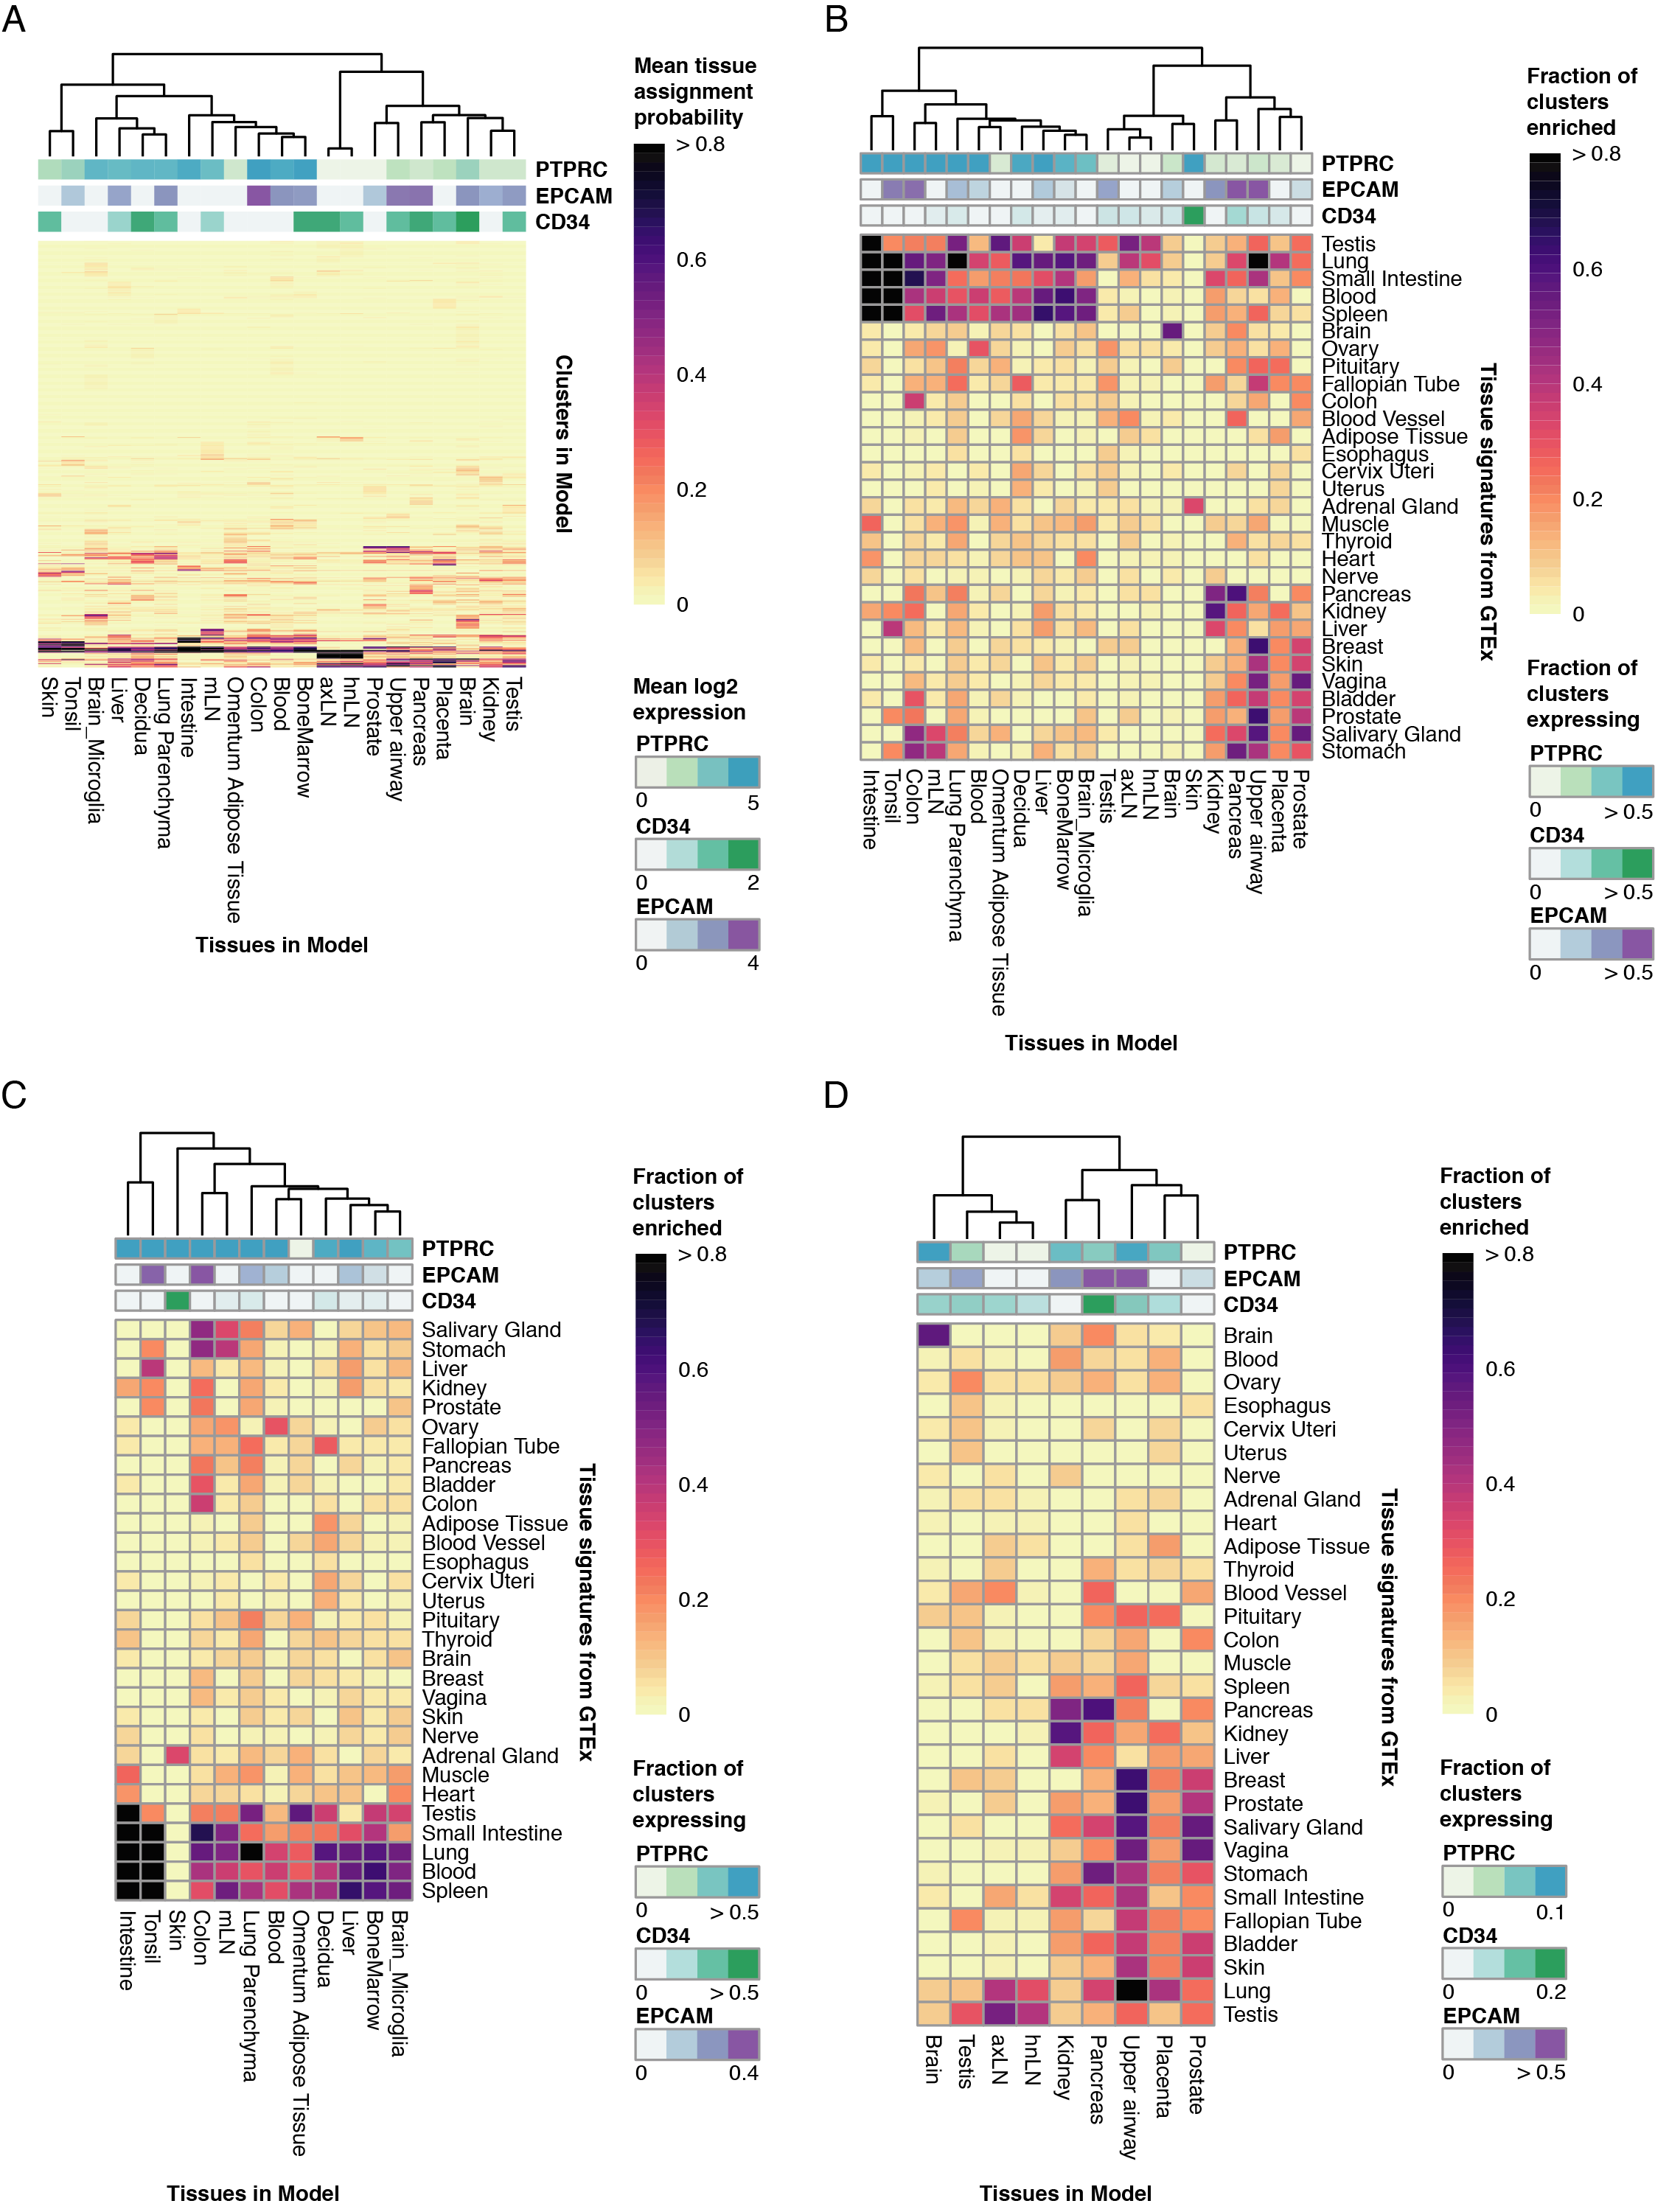
\includegraphics[scale=0.7185]{Chapter4/Figs/chap4_tissuefig.png} % change word in curlies to change figure
    \caption[Cell identity relationships across tissues]{\textbf{Cell identity relationships across tissues}\newline\textbf{(A)} Heatmap of the mean assignment probability of cells from a per-tissue cluster to the clusters of each given tissue in the dataset. \textbf{(B)} Heatmap of the fraction of clusters from a given tissue whose \textit{CellTypist} model signature is enriched in certain tissue-specific genes. \textbf{(C and D)} Two major branches of the column dendrogramme in (B), showing the immune enriched (C) and depleted (D) tissues. "Skin" was regrouped due to being an outlier grouped with the non-immune tissues in (B).}
    \label{fig:chap4_tiss}
\end{figure}

Tissue identity is also reflected in gene expression, and therefore in the genes with the top coefficients determined by the \textit{CellTypist} model. To unbiasedly probe the existence of tissue-specific signatures in the top genes of all clusters, tissue signatures were derived from the GTEx Consortium bulk RNA-seq dataset~\citep{consortium_genotype-tissue_2015} (see Methods Section~\ref{section4.4_genelists}). This provided an independent reference for tissue identity using gene expression. Inspection of tissue identity enrichment in cell clusters per tissue (Figure~\ref{fig:chap4_tiss}B) shows that, despite the sets of tissues in the \textit{CellTypist} and GTEx datasets not overlapping completely, matching between them is mostly concordant. Clustering of the enriched cluster fractions per tissue once again uncovered a similar picture as before, with a clear division between immune-enriched and immune-depleted tissues. The two cases that seem misaligned from \textit{PTPRC} expression - Omentum Adipose Tissue and Skin - both have an enrichment in immune cells. In the first, the low PTPRC fraction is likely derived from general low expression of this receptor. In the case of skin, the misclustering is likely related to the low number of clusters, as well as the specific cell types that make up the sample (Treg and Tmem cells~\citep{miragaia_single-cell_2019}). 

Tissues for which a large number of immune cells were obtained (either by biased sampling or biology) had more clusters enriched in signatures of lymphoid tissues  ("Blood", "Spleen"), as well as other barrier tissues, which potentially would include a greater number or activity of immune cells ("Lung", "Small intestine") (Figure~\ref{fig:chap4_tiss}C). The clustering of the profiled tissues (top dendrogramme of Figure~\ref{fig:chap4_tiss}C) revealed further relationships between them. Tonsil and intestine are grouped together likely due to their sampling bias: ILCs in tonsil, CD4\textsuperscript{+} T memory cells in intestine; and both of these cell types can have globally similar signatures. The clustering of liver and bone marrow is also expected, given that the vast majority of liver samples are from fetal origin, and reflect the organ's haematopoietic function at that stage of development. Lastly, the similarity between colon and the mesenteric lymph node (mLN) point towards a greater similarity between leukocyte populations present in both these tissues than with those from other tissues. However, an increase in sampling of immune cells from other lymph nodes and non-lymphoid tissues would further unravel their true relationships.

For the non-immune fraction (Figure~\ref{fig:chap4_tiss}D), cross tissue relationships could also be identified. Axilary (axLN) and head and neck (hnLN) lymph nodes were grouped together since both are uniquely sampled for endothelial cells only, in the same study~\citep{takeda_single-cell_2019}. They are outliers together with testis and brain, two tissues that have been repeatedly described has having very distinct transcriptomic profiles from other organs~\cite{brawand_evolution_2011,barbosa-morais_evolutionary_2012}. The brain clusters very uniquely match the "Brain" gene set, and clusters from testis are in their majority enriched for "Testis" signature as well as "Ovary". The remaining tissues grouped together show elevated enrichment in a group of signatures coming in their majority from barrier tissues ("Lung", "Bladder", "Skin", "Stomach", "Vagina"), as well as some tissues with secretory activity ("Salivary gland", "Prostate", "Breast"). This shows the difference in cellular function of these tissues compared with the immune group, and correlated with the functions of the tissues present (kidney, pancreas, upper airway, placenta and prostate).

The tissue relationships highlighted by the gene set enrichment directly derive from the \textit{CellTypist} model trained and the cell groupings that the pipeline defines. Examining other model alternatives shows that in some of them the tissue hierarchy is maintained (Figure~\ref{fig:appB_tissGSEA}), with the exception of the thr1 = 0.1, thr2 = 0.1 model. This is likely caused by excessive merging of clusters, leading to non-meaningful groupings and not so meaningful gene coefficients from the model.

%paragraph about the matching clusters
Plotting the clusters resulting from cross-tissue merging in \textit{CellTypist} can also reveal the similarity across tissues (Figure~\ref{fig:appC_tissrel}). As already shown by Figure~\ref{fig:appB_grids}A, the model with thr1 = 0.99 and thr2 = 0.8 is the one with the lowest number of merged clusters. We can however still observe clusters merging across tissues that have similar profiles and were included in the "immune enriched" group in Figure~\ref{fig:chap4_tiss}B - liver and bone marrow, lung parenchyma and intestine, decidua and omentum adipose tissue - as well as tissues that have functional associations - decidua and placenta, upper airway and lung parenchyma. The remaining models appear to maintain the occurrence of these associations between tissues, like the close clustering between axLN and hnLN, or the association of tissues including more immune sampling with blood and bone marrow. This is further underscored when the tissue gene signatures are examined in the merged clusters of each model (Figure~\ref{fig:appB_clmGSEA}). While the first model (thr1 = 0.99 and thr2 = 0.8) does not include enough merged clusters, both thr1 = 0.4 and thr2 = 0.99 and thr1 = 0.25 and thr2 = 0.25 again present the distinctive pattern of clustering the tissue signatures by the tissue functions as described before for the immune/non-immune partitions. This however is not evident for thr1 = 0.1 and thr2 = 0.1, likely due to excessive merging leading to a less meaningful model.

In conclusion, \textit{CellTypist} can reveal the relationships of cell identity across tissue, and relate it to a more structured hierarchy of cellular phenotypes (such as immune vs non-immune). However, this is also dependent of the profiled tissues, as well as how balanced the sampling of cell populations is in each tissue.


\subsection{Gene expression driving cell identity}
\label{section_genes}
Usage of logistic regression as a classification model in \textit{CellTypist} allows for a direct evaluation of the genes driving the classification for each cluster through their learned coefficients. With a comprehensive cell type reference, we can start to unravel what are the key determinants of cell identity across tissues.

\begin{figure}[pht!]
    \centering
    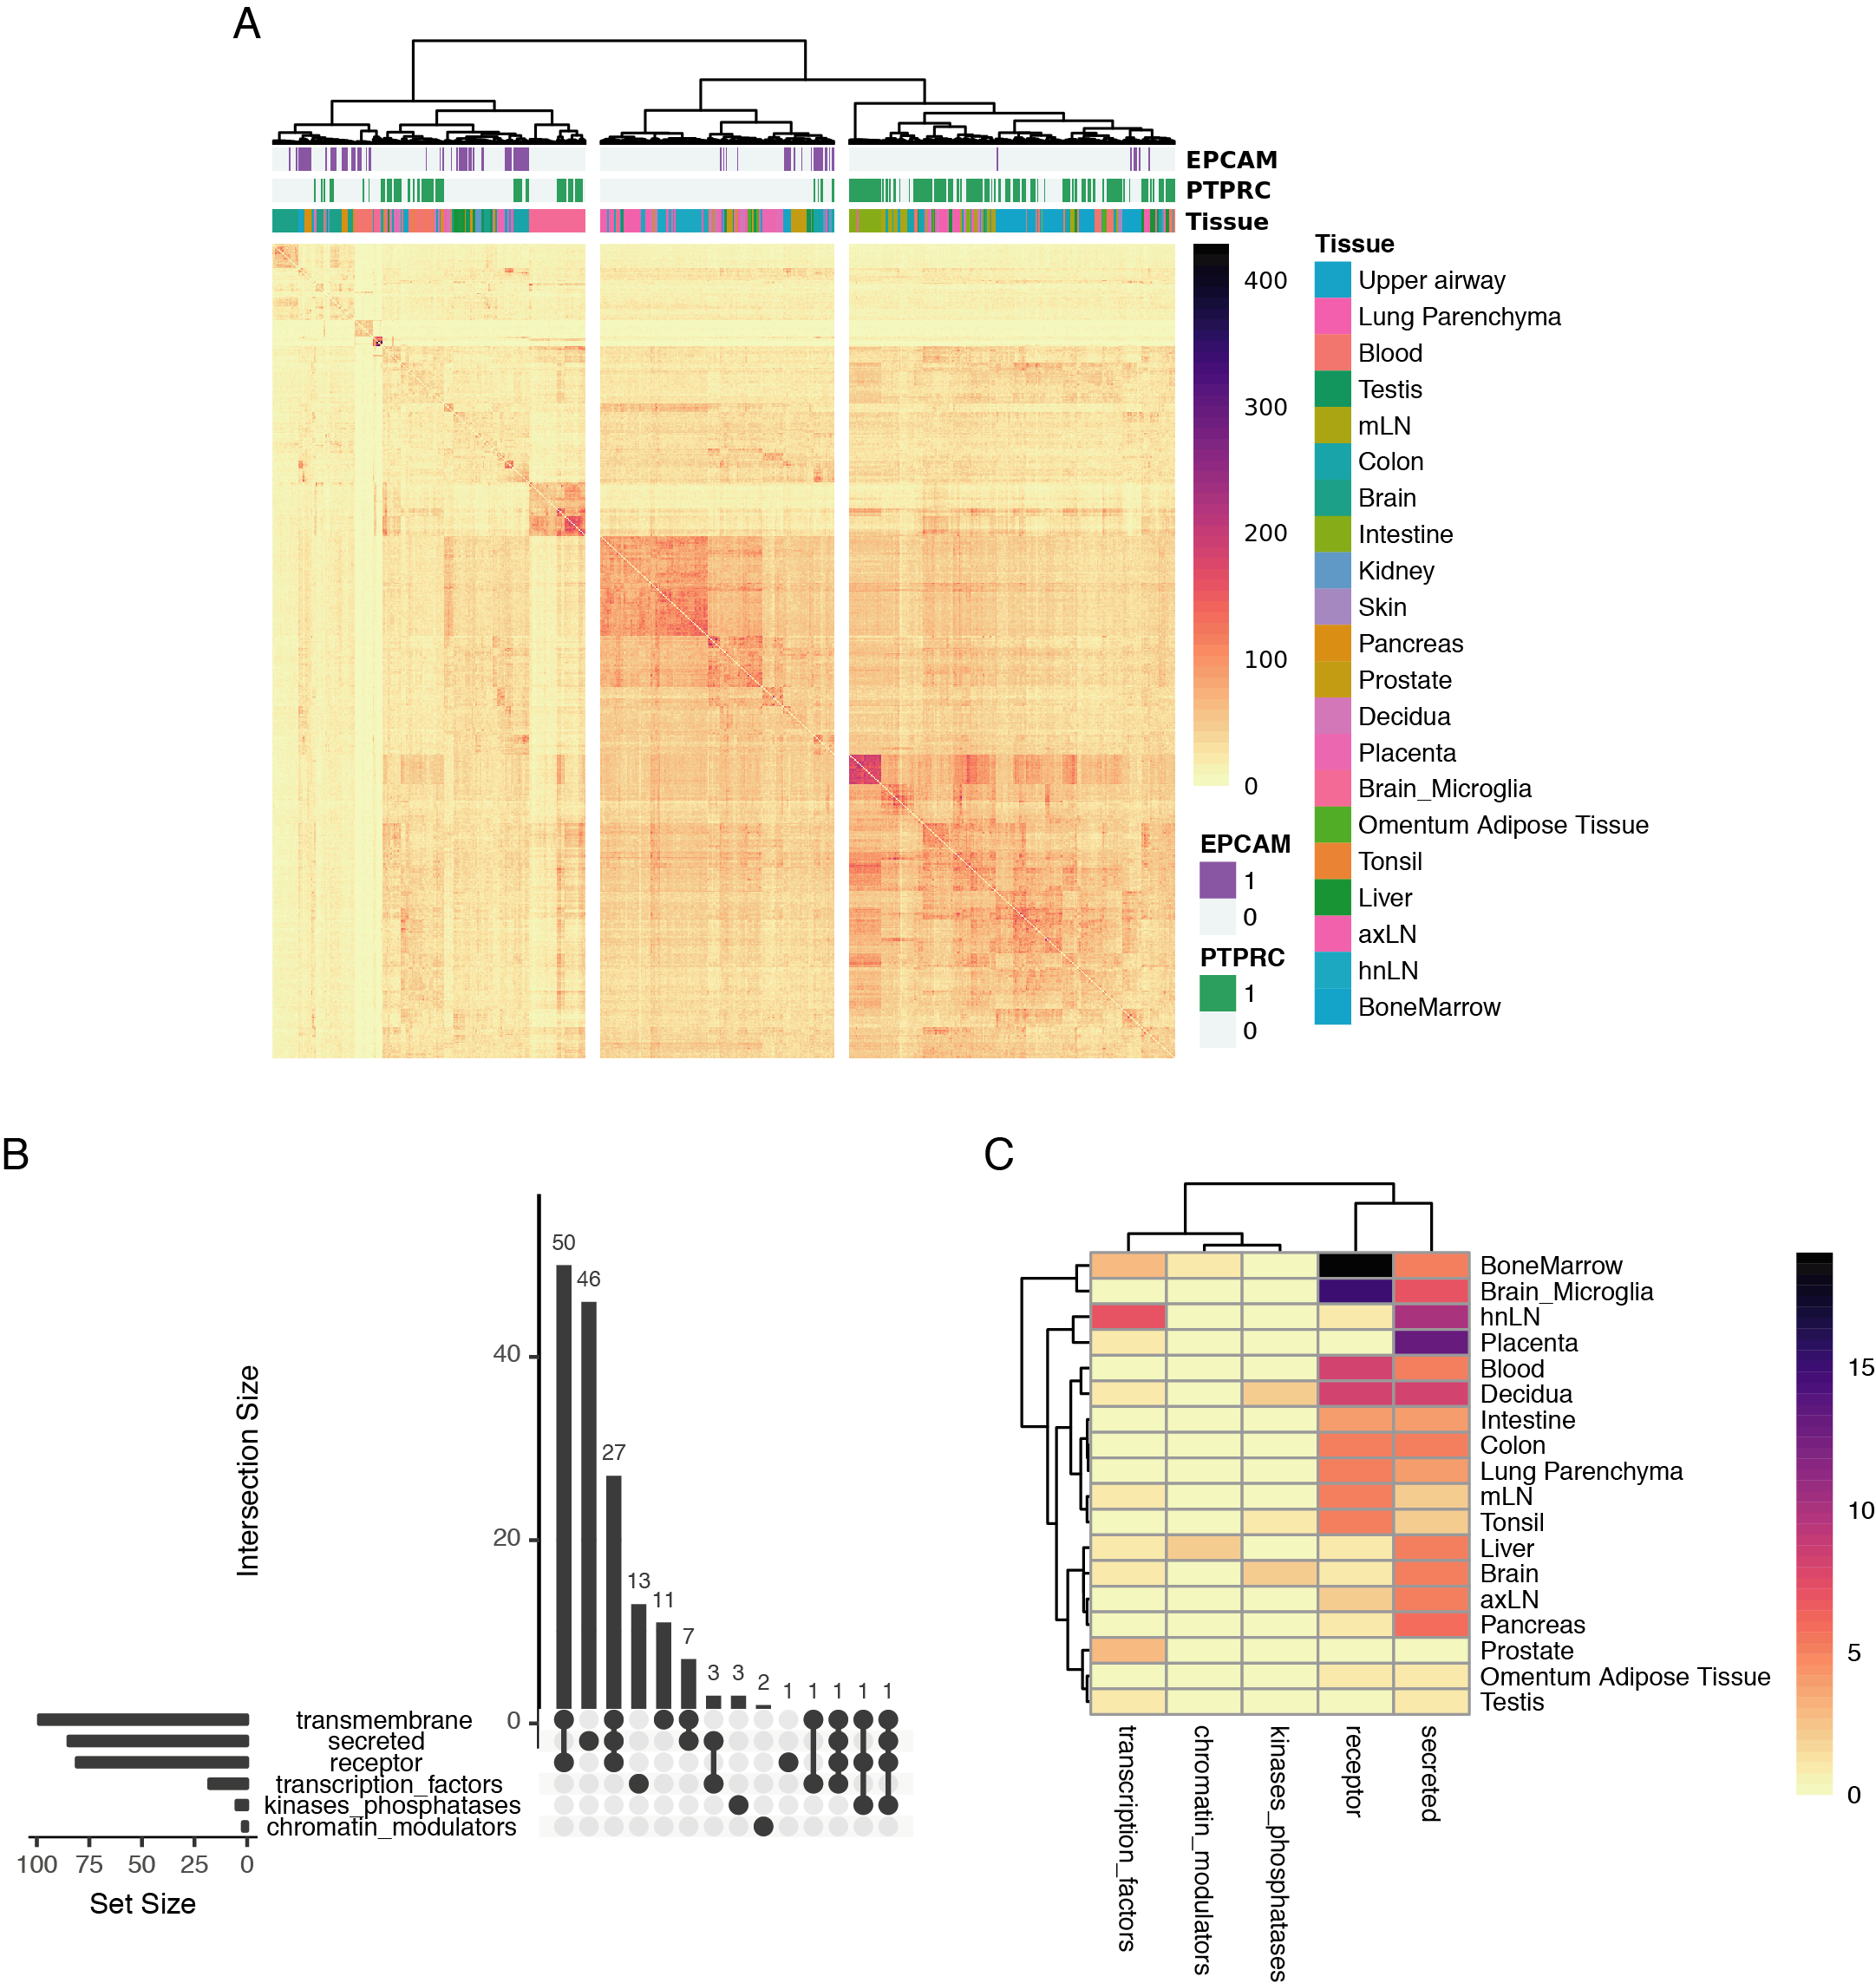
\includegraphics[scale=0.835]{Chapter4/Figs/chap4_genesAnalysis.png} % change word in curlies to change figure
    \caption[Genes driving cell identity definition across tissues]{\textbf{Genes driving cell identity definition across tissues}\newline\textbf{(A)} Clustered heatmap of the number of genes in common between pairs of \textit{CellTypist} clusters (thr1 = 0.99, thr2 = 0.8). Genes per cluster were determined as those with the top 500 coefficients as learned by the model. Values in the diagonal (number of genes per cluster, 500) were set to 0. \textbf{(B)} Upset plot counting the number of clusters enriched for a group of genes with a specific function. \textbf{(C)} Heatmap of number of clusters per tissue (y-axis) enriched for groups of genes with a specific function (x-axis). For panels (B) and (C), the gene groups tested were "transcription factors", "transmembrane", "secreted", "receptors", "membrane peripheral proteins", "kinases and phosphatases", "chromatin modulators", "catalytic enzymes", "housekeeping genes". Only the terms enriched in at least one cluster were shown.}
    \label{fig:chap4_genetypes}
\end{figure}

Relationships between clusters were probed by counting the number of pairwise shared genes. The top 500 genes were used to avoid a hard threshold across clusters, since the top coefficient values can be very variable between them. Clustering once more revealed a division between most immune and non-immune clusters (Figure~\ref{fig:chap4_genetypes}A). Moreover, various clusters containing cells from the same tissue were also grouped together, hinting at the existence of gene expression programmes shared by the different cell types within a tissue.

The concept of "cell type" is still inconclusively defined, yet it can be intimately related to a cell's molecular phenotype, i.e. the molecules driving cellular function. These drivers can either be the effector molecules directly responsible for the cell's array of functions, or the genomic regulators controlling the expression of genes involved in these functions. It has been showed that tissue-specificity at the gene expression level is mostly due to transcription factor-gene regulatory interactions~\citep{sonawane_understanding_2017}. The results from \textit{CellTypist} were used to assess what types of genes were more often at the top of the model coefficient rankings, which reflect the importance of expression of that gene in classifying a cell type. The following gene categories were tested for enrichment (see Methods Sections~\ref{section4.4_genelists} and~\ref{section4.4_enr}): Transcription Factors, Chromatin Modulators, Kinases and Phosphatases, Ligases and Deubiquitinases, Catalytic enzymes, Housekeeping genes, Receptors, Secreted proteins, Transmembrane proteins, and Peripheral membrane proteins. Analysis showed a consistent pattern for all surveyed models of predominantly enriched membrane and secreted proteins (Figure~\ref{fig:chap4_genetypes}B, Figure~\ref{fig:appB_supupset}). A number of clusters also had transcription factors enriched in their top hits, albeit in markedly lower number. Enrichment for the tested gene groups appeared evenly distributed across tissues, and did not group them in any meaningful manner (Figure~\ref{fig:chap4_genetypes}C). Lastly, it is also notable that only a fraction of the total clusters showed enrichment for any of the classes tested, which could be due to the restrictive test that only looks for enrichment at the very top genes, as well as the non-comprehensive list of functions tested.

These results point to the greater importance of the gene expression regulatory network's output molecules (genes coding for membrane and secreted proteins), in determining the identity of a cell.


\subsection{CellTypist as an operational reference for annotation}
\label{section_test}
% mention plans for a database
The operational goal of \textit{CellTypist} is to be used as an automatic classification framework for scRNA-seq data. Data integrated through the pipeline can be used as an unbiased model of cell identity to predict cell type labels in unannotated data.

\begin{figure}[pht!] 
\centering
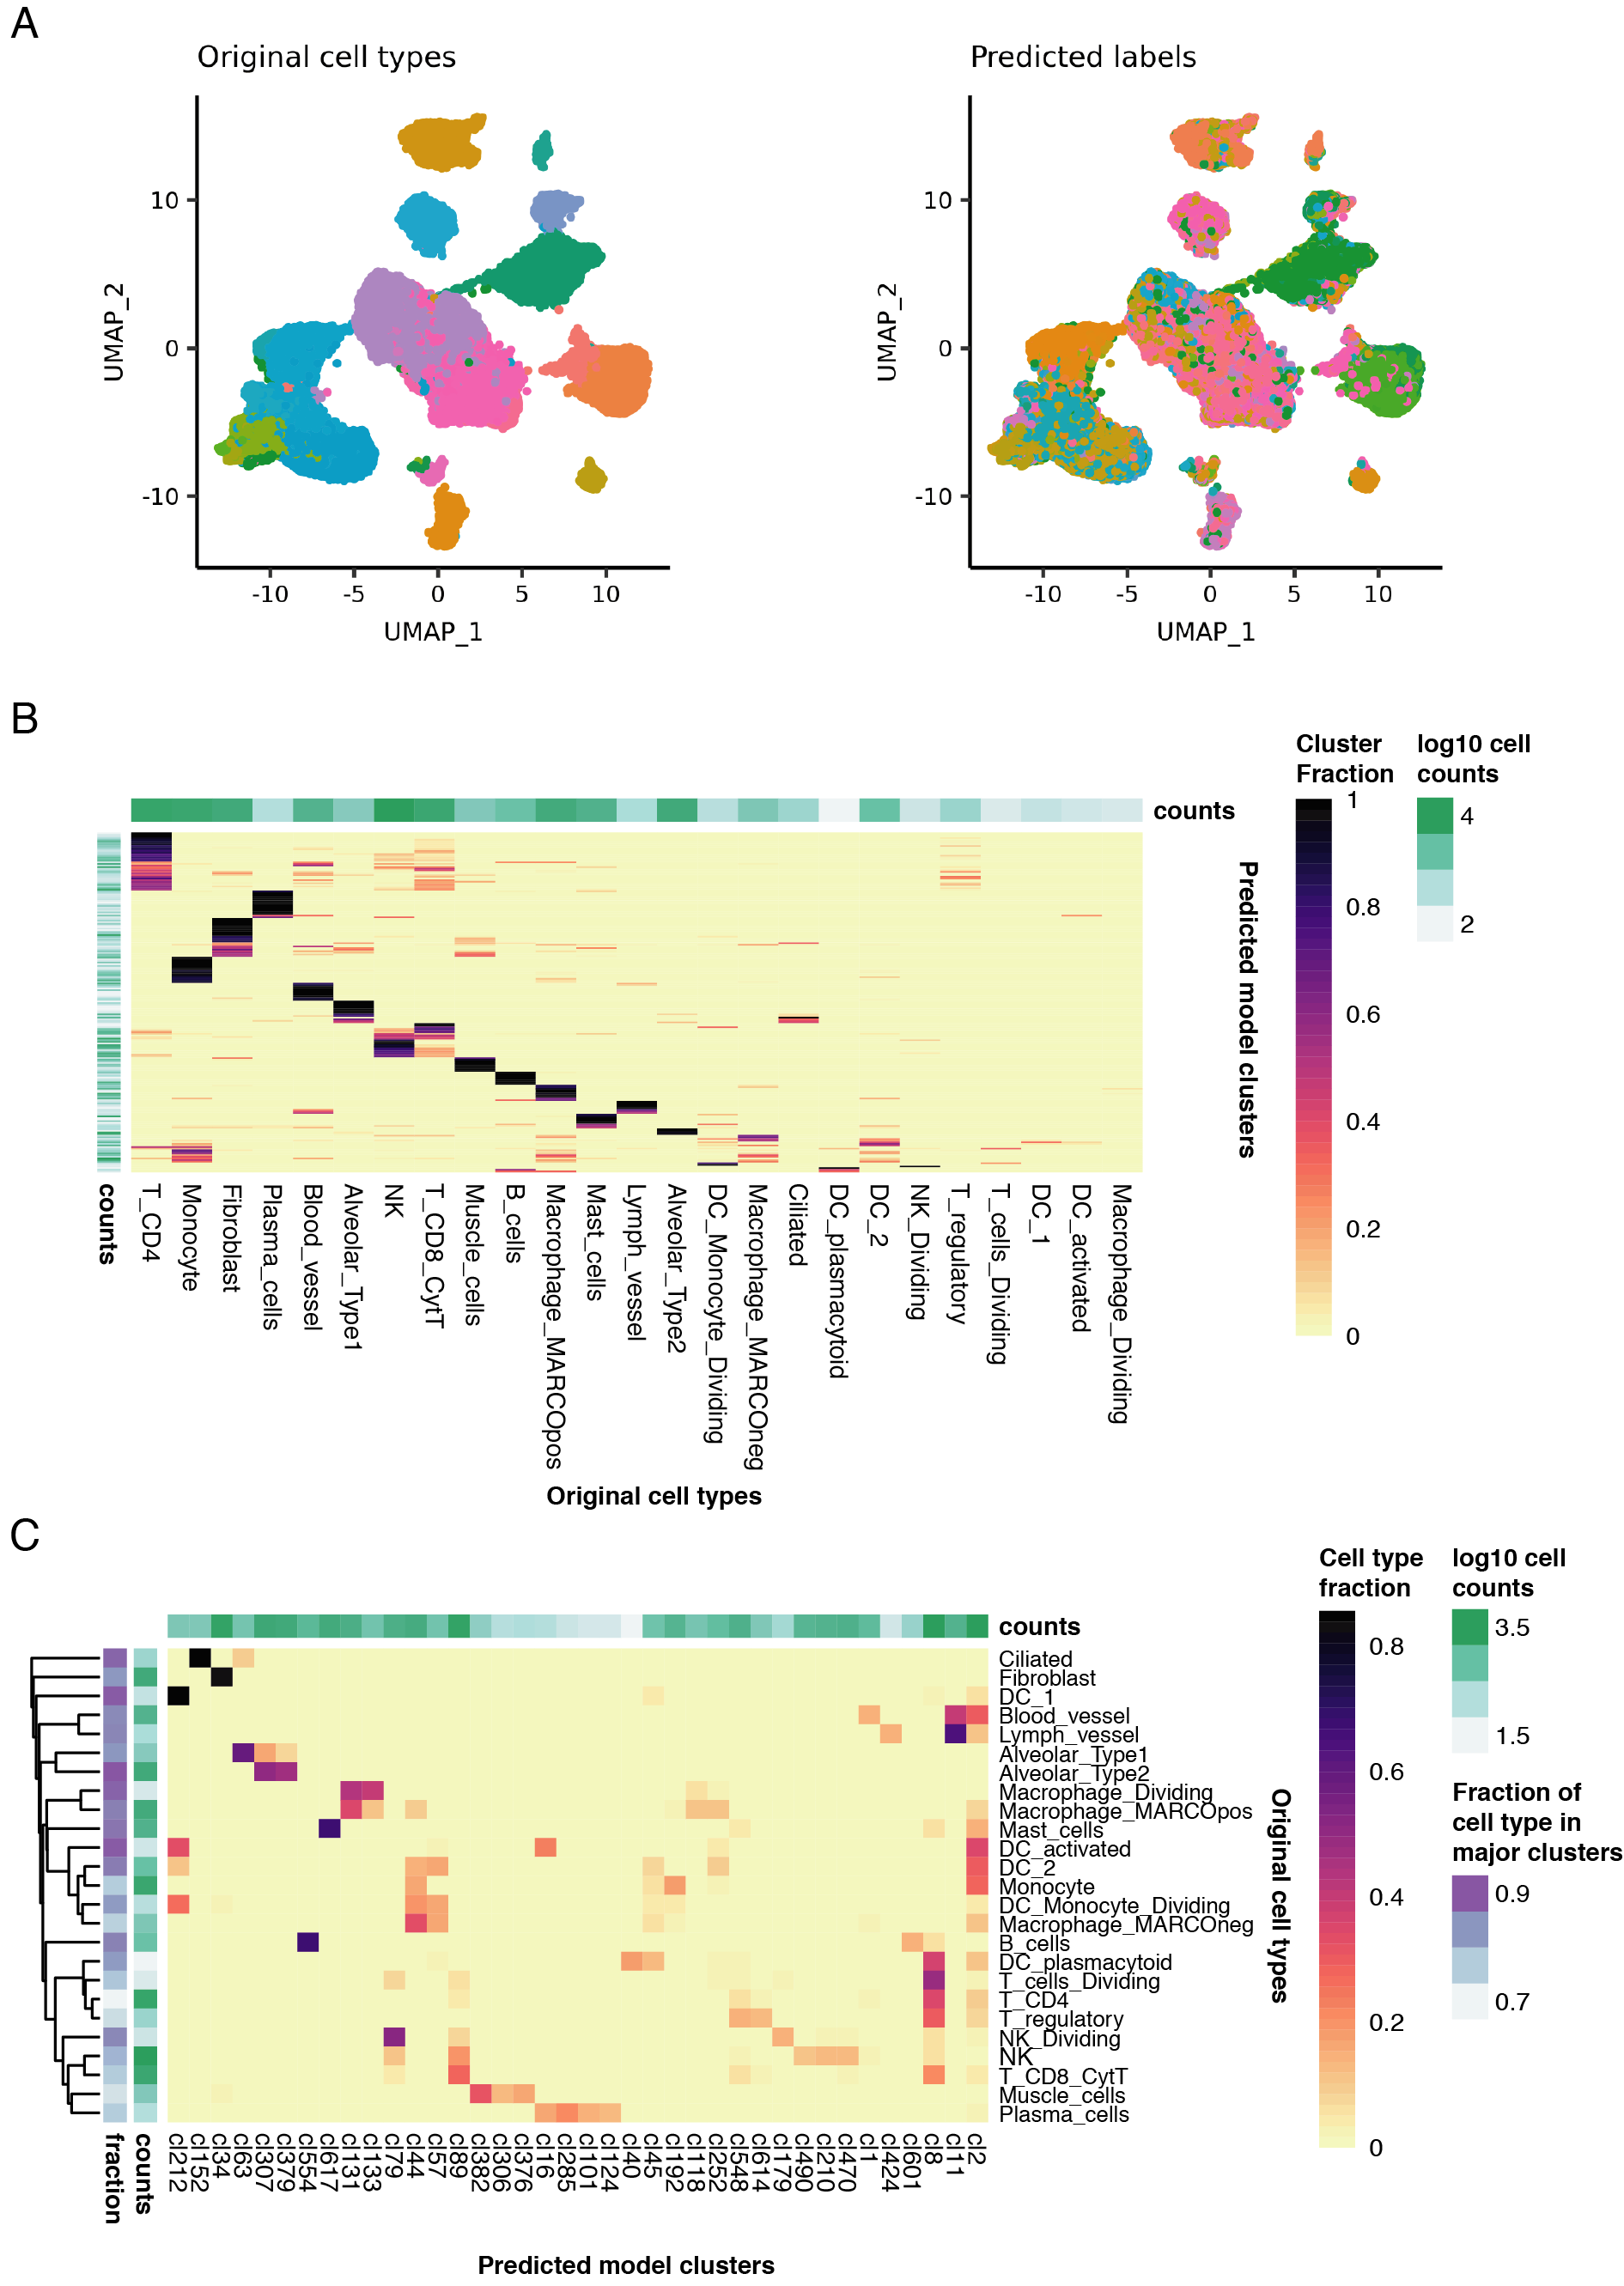
\includegraphics[scale=0.83]{Chapter4/Figs/chap4_preds.png} % change word in curlies to change figure
\caption[\textit{CellTypist} predictions for lung data from~\citep{madissoon_lung_2019}]{\textbf{\textit{CellTypist} predictions for lung data from~\citep{madissoon_lung_2019}}\newline\textbf{(A)} UMAP projections coloured by the original cell type annotations (left) and those predicted by \textit{CellTypist} (right) using thr1 = 0.99 and thr2 = 0.8. \textbf{(B)} Proportion of clusters (rows) matching each annotated cell type (columns). \textbf{(C)} Proportion of annotated cell types (rows) included in each cluster (columns). Only clusters including at least 10\% of a given cell type were included.}
\label{fig:chap4_preds}
\end{figure}

The data generated in~\citep{madissoon_lung_2019} was used to test the classification performance of \textit{CellTypist} with the compiled human data. This dataset was chosen because it includes three distinct tissues - lung, oesophagus, and spleen -, with only the first being represented in the collected datasets. More than 200.000 cells were collected from these three tissues, with various cell populations manually identified. The downside of this comparison is that the comparison can not be directly assessed, since the existing annotations for this dataset do not match those used by \textit{CellTypist}, which compiles a variety of nomenclatures used in each specific publication from where the data was obtained.

An overview of the classification results, projected in UMAP~\citep{mcinnes_umap:_2018} (Figure~\ref{fig:chap4_preds}A, Figure~\ref{fig:appB_oes}A, Figure~\ref{fig:appB_spleen}A), shows a similarity between the individual labelling of different clusters. The increased noise in \textit{CellTypist}'s annotations are likely due to the large number of categories it includes. Despite this, most model labels are highly specific, being attributed almost entirely to a single original cell type annotation (Figure~\ref{fig:chap4_preds}B, Figure~\ref{fig:appB_oes}B, Figure~\ref{fig:appB_spleen}B). While the opposite is not true (i.e. one cell type annotation can correspond to more than one cluster), it is nonetheless evident that each cell type is dominated by one or very few clusters (Figure~\ref{fig:chap4_preds}C, Figure~\ref{fig:appB_oes}C, Figure~\ref{fig:appB_spleen}C). Furthermore, even when excluding clusters including less than 10\% of cells from each annotated cell type (as is the case in the heatmap in Figure~\ref{fig:chap4_preds}C), the remaining clusters still include 70-90\% of cells (purple sidebar in Figure~\ref{fig:chap4_preds}C). 

A more careful look at the annotations present in the clusters that matched each original cell type in lung reveals the accuracy of the model. Type 2 alveolar cells matched clusters only containing that same annotation, whereas clusters in alveolar type 1 included type 1, and type 2, as well as secretory cells. Ciliated cells and fibrolasts mostly matched a single cluster each, in both cases composed of the exact same annotation. Cells annotated as "Lymph\_vessels" and "Blood\_vessels" both matched cl11 (containing "endothelium" and "lymphatic" cells), with the first also matching lymphatic endothelial cells from the axillary lymph node. T cell annotations were mostly assigned to cluster cl8, which includes a mix of CD4 and CD8 cells. In addition, T regulatory cells also matched cluster cl614, which includes activated T cells and Tregs. NK cells also matched a cluster with CD8 T cell annotation, but included two others containing mostly NK cells from other tissues. Lung cells that are derived from the myeloid lineage (Macrophages, Monocytes, Dendritic cells) all matched clusters mostly composed of these same annotations, albeit with some mix between them, which again demonstrates some of the difficulty that exists in separating these cell types.

% other models
The other models resulting from different parameters were also briefly examined. Despite the differences in number of clusters, all models show a similar specificity for the assigned clusters (Figure~\ref{fig:appB_othercl}). However, both models with fewer clusters (thr1 = 0.25, thr2 = 0.25; and thr1 = 0.1, thr2 = 0.1) both show less unique matching of original cell types to clusters (Figure~\ref{fig:appB_otherct}), with most of them matching the same larger clusters, which is likely an artifact of excessive merging within and across tissues (Figure~\ref{fig:chap3_combcl}A). 

Globally, it has been demonstrated that \textit{CellTypist} can be successfully used to annotate datasets with a broad diversity of cell types, and future improvements to the pipeline are likely to make it more precise in attributing cell identity. 


\section{Discussion}
\label{section4.3}
From its inception, the Human Cell Atlas (HCA) consortium has aimed to "define all human cell types in terms of distinctive molecular profiles (such as gene expression profiles)"~\citep{regev_human_2017}, a task that can not be easily accomplished by a single team. Beyond the financial and ethical constraints, collecting good quality scRNA-seq data requires tissue-specific knowledge, as well as profiling using both top-down and bottom-up approaches to obtain an overview of cell populations, while capturing cell type-specific phenotypic variations. Yet as data on human cells accumulates, methods capable of compiling the cellular census envisioned by the HCA members, and making it available to the community will be of great use.

% bias in collected data
%% model updating with new data will make it more inclusive/globally applicable
%% over represented cell types might "hide" smaller ones
%% data augmentation/downsampling can help
The human data presented provides a broad overview of several organs. This leads the cell type reference generated by \textit{CellTypist} to be broadly applicable to new datasets. This reference is dependent on the way these tissues are sampled. Currently, many of them are mostly or totally composed of immune cells which, while adding valuable information about their diverse phenotypes, can also bias the model. Collecting more datasets is the ideal way of mitigating this problem, but it can also be addressed by using data augmentation or downsampling approaches~\citep{wong_understanding_2016,hie_geometric_2019}. This would be especially relevant at the model training step, as we have observed the clear impact of number of cells per label in classification accuracy (Figure~\ref{fig:chap3_model}C, Figure~\ref{fig:chap3_modelcl}C, Figure~\ref{fig:chap4_HA}D).

Consistent data integration is also essential to avoid redundant classes and misleading interpretations about cell type and tissue relationships. Data integration for scRNA-seq is still a heavily studied topic~\citep{haghverdi_batch_2018,lopez_deep_2018,polanski_bbknn:_2019, stuart_comprehensive_2019}, and can considerably influence the cell groupings detected in the data. \textit{CellTypist} is likely to evolve as a pipeline, in order to adopt a within- and cross-tissue integration framework that closely reflects the cell type information available for each dataset.

%tissue biology
Tissue identity relationships appear as an emergent result from the application of \textit{CellTypist}. The associations revealed between tissues are present at the cross-tissue integration stage (Figure~\ref{fig:chap4_tiss}A), and then also reflected in the top genes learned by the logistic regression model (Figure~\ref{fig:chap4_tiss}B). Furthermore, tissue identity is to some degree robust to incorrect or excessive grouping of single-cells (Figure~\ref{fig:appB_tissGSEA}), which reveals that tissues-specific expression programmes might be intrinsic to the core cell identity. The resolution of these tissue connections and programmes can be improved by broader cell type sampling and integration. This will allow the model to reveal a more fine-grained hierarchy beyond the immune/non-immune split, and ultimately map cellular phenotypes to a structured cell identity atlas.

% gene biology
%% more detailed conclusions can be taken once the reference is uniformly annotated/if more annotated data is included (because we can now go beyond tissues/clusters to actual cell types)
%% discuss how more accurate gene groups can give more accurate results
The data compiled offers for the first time a window into the drivers of cell identity. Analysis of enriched gene expression programmes can be improved by using a more uniform gene reference, as well as adopting more informative labels for the clusters obtained (which can come from improved dataset merging or manual annotation). Nonetheless, the analysis showed consistently ranked receptors and secreted molecules above transcription factors when defining cell identity (Figure~\ref{fig:chap4_genetypes}B, Figure~\ref{fig:appB_supupset}). This is in agreement with previous reports~\citep{sonawane_understanding_2017}, yet this is the first instance where this type of analysis could achieve this level of cell type resolution. Importantly, defining which genes make up the core of cellular phenotypes is not the same as defining cell identity regulation. However, knowledge of the minimal gene expression set required to classify or obtain a determined phenotype (and consequently function) is a key point in understanding the operational definition of cell types. Thus, the expansion and improvement of the \textit{CellTypist} reference will increasingly provide a foundation to understanding how cell types arise and evolve~\citep{zimmermann_ancient_2019}, and will help prioritise gene targets for effective cellular engineering.

% use and availability of this data collection
This large human cell type reference can be very useful to characterise cell identity in a variety of systems. In disease-focused studies, the steady-state reference provided by \textit{CellTypist} can automatically annotate the cells obtained from a disease sample, eliminating the need to obtain a matching healthy sample. Another potential use is to characterise cell fates and heterogeneity when differentiating organoids. Classifying scRNA-seq data from the generated organoids using an unbiased reference can reveal the cell types present that a specific protocol was able to differentiate. \textit{CellTypist} will also be available as an online resource, where the model can be directly used, and is accompanied by a database showing the defining characteristics of each cell type - marker genes detected, tissues of origin, datasets characterising them, and similar cell types. This is further intended to be articulated with a Cell Ontology~\citep{bard_ontology_2005}, and have cell names be consistently used when new data is produced, with a direct correspondence to both databases. Lastly, future releases of \textit{CellTypist} models will include more species, adding an evolutionary layer to our knowledge of cell identity.


\section{Methods}
\label{section4.4}
\subsection{\textit{CellTypist} parameter optimisation and training}
\label{section4.4_model}
The \textit{CellTypist} pipeline was applied to the complete human dataset. Data from the same tissues was integrated and clustered using the Leiden algorithm~\citep{traag_louvain_2019} at several resolutions. For tissues with cell type annotations, resolution was optimised using the split-join distance~\citep{dongen_performance_2000} between clusters and cell type annotation and constrained to a number of clusters at least as large as the number of cell type annotations in the largest collected dataset (Figure~\ref{fig:chap4_HA}A, see also Chapter~\ref{chap:CT_method} Section~\ref{section3.2.1}).

Following clustering, per tissue logistic regression models were trained, running for 10 epochs of a maximum of 100 iterations each. These models were used to run the cross-tissue cluster merging pipeline (Chapter~\ref{chap:CT_method} Section~\ref{section3.2.2}), and a combination of parameters was chosen based on the ratio of split-join distances (merged vs annotated cell types over per tissue vs annotated cell types) (Figure~\ref{fig:chap4_HA}B), resulting in the choice of thr1 = 0.99 and thr2 = 0.8. Additionally, three other combinations were chosen for comparison: thr1 = 0.4 and thr2 = 0.99, the combination with the top split-join ratio when only considering merged clusters (Figure~\ref{fig:appB_grids}C, Figure~\ref{fig:appB_moremodels}A-B); thr1 = 0.25 and thr2 = 0.25, one of the combinations with the highest fraction of merged clusters (Figure~\ref{fig:appB_grids}B, Figure~\ref{fig:appB_moremodels}C-D); thr1 = 0.1 and thr2 = 0.1, the combination with the highest fraction of merged clusters, as well as highest split-join fraction (Figure~\ref{fig:appB_grids}B, Figure~\ref{fig:appB_moremodels}E-F).

The groupings obtained were used to train a logistic regression model using Stochastic Gradient Descent (Chapter~\ref{chap:CT_method} Section~\ref{section3.2.3}). Training was done for 25 epochs of a maximum of 100 iterations each, where in each iteration 1000 cells were seen by the model. 90\% of the total data was used as a training set, and the remaining as a left out test set that was tested at every iteration (Figure~\ref{fig:chap4_HA}C-D, Figure~\ref{fig:appB_moremodels}).


\subsection{Obtaining gene group lists}
\label{section4.4_genelists}
The groups of genes here presented were chosen to reflect various broad functions present in cells. They are not exhaustive, and overlaps between gene sets exist due to the ambiguity of some categories. In some tests, various categories were used, yet only those with at least one positive result were reported (Figure~\ref{fig:chap4_tiss}B, Figure~\ref{fig:chap4_genetypes}B).

\textit{GO Terms}: GO Terms were downloaded using the biomaRt R package~\citep{durinck_mapping_2009}. Genes from different terms were then grouped in the following categories (similar to~\citep{hagai_gene_2018}): chromatin modulators (GO:0006338 (chromatin remodelling), GO:0003682 (chromatin binding), GO:0042393 (histone binding), and GO:0016568 (chromatin modification)); kinases and phosphatases (GO:0004672 (protein kinase activity) and GO:0004721 (phosphoprotein phosphatase activity)) and catalytic enzymes (GO:0003824 (catalytic activity)).

\textit{Transcription Factors}: Human transcription factors were obtained from AnimalTFDB v3.0 (~\url{http://bioinfo.life.hust.edu.cn/AnimalTFDB/})~\citep{hu_animaltfdb_2019}.

\textit{Housekeeping genes}: Housekeeping genes were obtained from~\url{https://m.tau.ac.il/~elieis/HKG/}~\citep{eisenberg_human_2013}.

\textit{Cell communication-associated genes}: Genes involved in cell-cell communication were obtained from~\url{cellphonedb.org}~\citep{efremova_cellphonedb_2019}. Only genes annotated as "transmembrane", "secreted", "peripheral", and "receptor" were kept. Given the structure of the annotation in this database, some genes are included in more than one group. In particular, most receptors and some secreted proteins are also classified as transmembrane.

\textit{Tissue-specific genes}: Tissue specific genes were determined as described in~\citep{sonawane_understanding_2017}. Briefly, RNA-seq expression data from the GTex Consortium was obtained (~\url{https://gtexportal.org/home/index.html})~\citep{consortium_genotype-tissue_2015}, and genes were considered tissue-specific for a given tissue if the difference between their median expression in that tissue and across all tissues normalised by its interquartile range across all tissues, was greater than 2.


\subsection{Enrichment of gene groups}
\label{section4.4_enr}
To obtain enriched groups of genes (Sections~\ref{section_tissues} and~\ref{section_genes}), the top 500 genes based on their model coefficients were obtained for each cluster. Gene Set Enrichment Analysis (GSEA)~\citep{subramanian_gene_2005} was performed using the liger R package (\url{https://cran.rstudio.com/web/packages/liger/index.html}), considering the gene sets as defined in Section~\ref{section4.4_genelists}. Enrichment was deemed signifficant if the q-value was lower than 0.05, and if the enrichment score was positive, signifying an enrichment in the top genes. In heatmaps plotting GSEA results (Figure~\ref{fig:chap4_tiss}B-D; Figure~\ref{fig:appB_tissGSEA}), the colour scale is capped at 0.8 (fraction of enriched clusters per tissue), and the annotation scales are capped at 0.5 (fraction of clusters with mean expression of the indicated gene of at least 1). Clusters merge across tissues were only counted towards the tissue contributing the most cells to them.



%!TEX root = ../thesis.tex
%*******************************************************************************
%****************************** Fifth Chapter **********************************
%*******************************************************************************
\chapter{Concluding remarks} \label{chap:conc}

% **************************** Define Graphics Path **************************
\ifpdf
    \graphicspath{{Chapter5/Figs/Raster/}{Chapter5/Figs/PDF/}{Chapter5/Figs/}}
\else
    \graphicspath{{Chapter5/Figs/Vector/}{Chapter5/Figs/}}
\fi
Developments in single-cell genomics are still shaping the way we define cellular identity. With the increasing number of cell types, organs and species profiled, we are bound to obtain an exhaustive overview of eukaryotic cell diversity, together with their genomic determinants. This work illustrates the importance of studying cell types across different tissues, and discussed computational challenges as well as solutions for the integrative atlasing of cellular diversity.

\section{Cells and genes trade-offs in single-cell profiling}
\label{section_prof}
% changes in number of cells
The number of cells profiled per study is still increasing exponentially~\citep{svensson_exponential_2018}. This has been accompanied by a marked expansion in the number of studies using single-cell technologies~\citep{svensson_curated_2019}, much of it due to the spread in use of a more standardised cell isolation and sequencing pipeline, 10x Genomics' Chromium technology. This democratisation of single-cell omics is resulting in more cell types, tissues and species being profiled. Nevertheless, single-cell studies should be designed with a clear goal, and the choice of protocol should be adequate to the question at hand.

% changes in protocol (full length, 3', 5') - why?
With regards to the type of sequencing, scRNA-seq protocols can be broadly split between full length transcript profiling and 5'/3' RNA tagging. Full length protocols - the most widely used being Smart-seq2~\citep{picelli_full-length_2014} - follow in the footsteps of the majority of bulk RNA-seq studies. Smart-seq2 is still dependent on mRNA isolation by the poly-A tail, and thus does not reveal changes in non-polyadenylated transcript as other protocols might~\citep{hayashi_single-cell_2018,verboom_smarter_2019}. Despite this, Smart-seq2's full length characteristics have been important to study immune cells. The development of TraCeR~\citep{stubbington_t_2016} and BraCeR~\citep{lindeman_bracer:_2018} have allowed the detection of TCR and BCR transcripts in single-cell data, which in turn have been used to lineage trace T cells with similar developmental origin~\citep{lonnberg_single-cell_2017} and Treg cell migration between tissues~\citep{miragaia_single-cell_2019} (Chapter~\ref{chap:Treg}). Smart-seq2 has also allowed uncovering the diversity of KIR receptors in NK cells at the maternal-fetal interface~\citep{vento-tormo_single-cell_2018}. Splicing-oriented studies with this protocol, on the other hand, have been scarce~\citep{arzalluz-luque_single-cell_2018}, yet splicing can be important in revealing important features of cell identity. Combination of Chromium and PacBio long read sequence has revealed cell type specific isoforms in mouse cerebellum~\citep{gupta_single-cell_2018}. Other changes in isoform usage also exist that can influence cell identity, yet this has been underappreciated.

% more cells/more reads?
The dominance of 3' and 5' sequencing protocols stems from the fact that a large number of cells is more important to reveal of cell diversity in a given tissue or condition than increased sequencing depth or number of genes per cell~\citep{svensson_quantifying_2019}, which has been showed early on when profiling bipolar retinal cells in mouse~\citep{shekhar_comprehensive_2016}. Droplet-based protocols allow the user to more easily isolate a large number of cells, which are then only sequenced at lower levels. This increase in cell numbers was necessary in the Treg cell work presented in Chapter~\ref{chap:Treg} to detect the subpopulations composing the lymph node-peripheral tissue trajectory (Figures~\ref{fig:chap2_fig2} and~\ref{fig:chap2_fig3}). Thus, at the transcriptomic level, different protocols can serve complementary functions - either increasing the resolution of the cellular census, or provide a more detailed representation of the molecular makeup of cell populations.


\section{Building a transcriptomic atlas of cell types}
\label{section_atlas}
The study presented in Chapter~\ref{chap:Treg} shows that, to unravel the full extent of cell identity, it is not enough to unbiasedly profile a tissue, since even low-frequency cell populations may reveal functional heterogeneity. Furthermore, the relevance of this is sometimes only apparent once more tissue-specific context is added. In isolation, the census of colonic Treg cells would only reveal different levels of activation, but once this was combined with the draining mesenteric lymph node (mLN) populations, and compared with Treg cells in the brachial lymph nodes, it became clear that these subpopulations formed a continuum across organs, and the subpopulations present in the mLN expressed genes that coded for homing chemokine receptors specific for the colon.

%types of atlases (RNA, ATAC, regulation, spatial)
The development of single-cell sequencing methods has unlocked the ability to perform unbiased cellular phenotyping. Yet there are several layers, from DNA, RNA and protein, to probe this phenotype. From these, at the single-cell level, RNA is by far the most widely available. While it is not as close to cellular function as proteins, it nonetheless has a very good approximation, and can be unbiasedly amplified. The spread of cellular transcriptomic profiling was not initially accompanied by a development of dedicated databases for this type of data, although more recent efforts have been made towards this end~\citep{alavi_web_2018,franzen_panglaodb:_2019}, and is the goal of the Human Cell Atlas to gather and standardise single-cell expression data. Moreover, most of the data produced is not accompanied by cell type annotations in a machine-readable format, nor does it follow a standardised nomenclature. This is likely because the existing ontologies~\citep{bard_ontology_2005} were not prepared for this explosion in cell profiling and the diversity of cell types and states it brought. Thus, the existence of these scRNA-seq datasets creates an opportunity to develop and update an informed cell type reference~\citep{aevermann_cell_2018}. Chapter~\ref{chap:CT_method} introduced \textit{CellTypist}, a method to integrate scRNA-seq data from multiple sources and tissues. This pipeline does not require a uniform annotation \textit{a priori}, and produces an interpretable model for annotation of new data.

While most cell population profiling focus on RNA, other aspects are also relevant. Open chromatin regions are easily identifiable through scATAC-seq. These regions are often involved in regulation of gene expression, and have been shown to be sufficient to distinguish cell types similarly to expression profiling~\citep{cusanovich_single-cell_2018}. An open chromatin cell type atlas can then provide a more regulatory perspective of cell identity, perhaps more clearly illustrating what effective alterations at the DNA level result in acquisition or loss of cellular phenotypes.

%what to they teach us?
% mention the uses
Cell type references like \textit{CellTypist} have a multitude of applications, ranging from basic science to applied biomedicine. The predictive capabilities of this sort of models can be used to test cellular responses in organoids~\citep{brazovskaja_high-throughput_2019}. This assessment can range from evaluating the differentiation potential of cultured cells, to measuring deviations and responses caused by external factors, like varying differentiation molecules or infectious agents. Ultimately, this can further improve the efforts in the field of tissue engineering, by guiding the development of \textit{in vitro} differentiation protocols~\citep{camp_single-cell_2018}. Likewise, these references can also be used in a clinical setting to probe changes in cell diversity in disease. In cancer, infiltration and phenotypic changes of immune cells can be assessed, and single-cell phenotyping of tumour cells can monitor its progression. Monitoring of cell abundances and diversity in the clinic can provide a new view of disease from a "cell ecology" perspective.

More fundamentally, \textit{CellTypist} as an integrated, cross-tissue cell type compendium can inform us on the drivers and underlying structure of cell identity.


\section{Defining cellular identity}
\label{section_ident}
% how can cellular identity be defined?
%% function? morphology? spatial? molecular phenotype? developmental?
%% how are these measured?
The advent of single-cell genomics has re-ignited the debate on the definition of cell type identity. Historically, cell types have been defined based on their morphology, location, function, or developmental origin. Development of cellular staining, and especially flow cytometry, have added molecular phenotyping to this list. While flow cytometry already offered a large cell throughput capable of detecting even the smallest populations, the revolutionary aspect of single-cell transcriptomics has been the unbiased probing of RNA molecules, revealing a hitherto obscured cellular map of gene expression programmes.

% role of multi-omics
It is only through integration that we can achieve a organism-scale picture of cell identity. This is achieved by \textit{CellTypist}, which is capable of resolving cell type correspondences across tissues (Figure~\ref{fig:chap3_pertiss}, Figure~\ref{fig:chap4_tiss}), and provide the list of genes at the core of each cell grouping (Figure~\ref{fig:chap4_genetypes}). Despite the discussed limitations, owed in part to the still limited diversity of data available, \textit{CellTypist} can lay the groundwork to reveal the first systematic picture of human cell types (with an expansion to other species in sight).

The transcriptomic composition of cells is vastly informative for their taxonomy, yet  only makes up a small portion of the information we can obtain. Other omics modalities (open chromatin, chromatin modifications, methylation, proteomics, ...) can provide equally informative yet complementary perspectives on cellular identity. Furthermore, these can be integrated computationally~\citep{stuart_comprehensive_2019} or obtained simultaneously using appropriate protocols~\citep{angermueller_parallel_2016,clark_scnmt-seq_2018}. Nonetheless, an ideal compendium of cell types should strive to go beyond this low level and invasive characterisation, and merge back into the knowledge obtained from other modalities. Cellular interactions are of great importance to cell function, and thus spatial information adds a relevant layer to this. Mapping the developmental trajectories of all cell types can inform us on their origin and generative processes. Morphology is the most easily observed characteristic, and heavily related to cell function, thus controlled by the genome. Only through integration can this systems view of cell biology come to fruition.

% cell type vs cell state
When possessing information on these many layers of cell phenotypes, we will be able to more accurately define the boundary between cell types and cell states. Often these can be observed in each individual modality - transient versus definitive cell shapes, immune lineages and their response to pathogens, or intermediate versus leaf stages in cellular differentiation. Yet these perspectives need each other, as cellular form and function should be understood in the context of its origin and genomic programming. Reconciling these different perspectives through a multi-window approach will provide us with a complete blueprint of the basic unit of life. It is expected that the unified view provided by the Human Cell Atlas - and indeed all cell atlases - results in a Modern Synthesis of Cell Theory.




% ********************************** Back Matter *******************************
% Backmatter should be commented out, if you are using appendices after References
%\backmatter

% ********************************** Bibliography ******************************
\begin{spacing}{0.9}

% To use the conventional natbib style referencing
% Bibliography style previews: http://nodonn.tipido.net/bibstyle.php
% Reference styles: http://sites.stat.psu.edu/~surajit/present/bib.htm

\bibliographystyle{apalike}
%\bibliographystyle{unsrt} % Use for unsorted references  
%\bibliographystyle{plainnat} % use this to have URLs listed in References
\cleardoublepage
\bibliography{References/references} % Path to your References.bib file


% If you would like to use BibLaTeX for your references, pass `custombib' as
% an option in the document class. The location of 'reference.bib' should be
% specified in the preamble.tex file in the custombib section.
% Comment out the lines related to natbib above and uncomment the following line.

%\printbibliography[heading=bibintoc, title={References}]


\end{spacing}

% ********************************** Appendices ********************************

\begin{appendices} % Using appendices environment for more functionality

%!TEX root = ../thesis.tex
% ******************************* Thesis Appendix A ****************************
\chapter{How to install \LaTeX} 

\section*{Windows OS}

\subsection*{TeXLive package - full version}
\begin{enumerate}
\item	Download the TeXLive ISO (2.2GB) from\\
\href{https://www.tug.org/texlive/}{https://www.tug.org/texlive/}
\item	Download WinCDEmu (if you don't have a virtual drive) from \\
\href{http://wincdemu.sysprogs.org/download/}
{http://wincdemu.sysprogs.org/download/}
\item	To install Windows CD Emulator follow the instructions at\\
\href{http://wincdemu.sysprogs.org/tutorials/install/}
{http://wincdemu.sysprogs.org/tutorials/install/}
\item	Right click the iso and mount it using the WinCDEmu as shown in \\
\href{http://wincdemu.sysprogs.org/tutorials/mount/}{
http://wincdemu.sysprogs.org/tutorials/mount/}
\item	Open your virtual drive and run setup.pl
\end{enumerate}

or

\subsection*{Basic MikTeX - \TeX~ distribution}
\begin{enumerate}
\item	Download Basic-MiK\TeX (32bit or 64bit) from\\
\href{http://miktex.org/download}{http://miktex.org/download}
\item	Run the installer 
\item	To add a new package go to Start >> All Programs >> MikTex >> Maintenance (Admin) and choose Package Manager
\item	Select or search for packages to install
\end{enumerate}

\subsection*{TexStudio - \TeX~ editor}
\begin{enumerate}
\item	Download TexStudio from\\
\href{http://texstudio.sourceforge.net/\#downloads}
{http://texstudio.sourceforge.net/\#downloads} 
\item	Run the installer
\end{enumerate}

\section*{Mac OS X}
\subsection*{MacTeX - \TeX~ distribution}
\begin{enumerate}
\item	Download the file from\\
\href{https://www.tug.org/mactex/}{https://www.tug.org/mactex/}
\item	Extract and double click to run the installer. It does the entire configuration, sit back and relax.
\end{enumerate}

\subsection*{TexStudio - \TeX~ editor}
\begin{enumerate}
\item	Download TexStudio from\\
\href{http://texstudio.sourceforge.net/\#downloads}
{http://texstudio.sourceforge.net/\#downloads} 
\item	Extract and Start
\end{enumerate}


\section*{Unix/Linux}
\subsection*{TeXLive - \TeX~ distribution}
\subsubsection*{Getting the distribution:}
\begin{enumerate}
\item	TexLive can be downloaded from\\
\href{http://www.tug.org/texlive/acquire-netinstall.html}
{http://www.tug.org/texlive/acquire-netinstall.html}.
\item	TexLive is provided by most operating system you can use (rpm,apt-get or yum) to get TexLive distributions
\end{enumerate}

\subsubsection*{Installation}
\begin{enumerate}
\item	Mount the ISO file in the mnt directory
\begin{verbatim}
mount -t iso9660 -o ro,loop,noauto /your/texlive####.iso /mnt
\end{verbatim}

\item	Install wget on your OS (use rpm, apt-get or yum install)
\item	Run the installer script install-tl.
\begin{verbatim}
	cd /your/download/directory
	./install-tl
\end{verbatim}
\item	Enter command `i' for installation

\item	Post-Installation configuration:\\
\href{http://www.tug.org/texlive/doc/texlive-en/texlive-en.html\#x1-320003.4.1}
{http://www.tug.org/texlive/doc/texlive-en/texlive-en.html\#x1-320003.4.1} 
\item	Set the path for the directory of TexLive binaries in your .bashrc file
\end{enumerate}

\subsubsection*{For 32bit OS}
For Bourne-compatible shells such as bash, and using Intel x86 GNU/Linux and a default directory setup as an example, the file to edit might be \begin{verbatim}
edit $~/.bashrc file and add following lines
PATH=/usr/local/texlive/2011/bin/i386-linux:$PATH; 
export PATH 
MANPATH=/usr/local/texlive/2011/texmf/doc/man:$MANPATH;
export MANPATH 
INFOPATH=/usr/local/texlive/2011/texmf/doc/info:$INFOPATH;
export INFOPATH
\end{verbatim}
\subsubsection*{For 64bit OS}
\begin{verbatim}
edit $~/.bashrc file and add following lines
PATH=/usr/local/texlive/2011/bin/x86_64-linux:$PATH;
export PATH 
MANPATH=/usr/local/texlive/2011/texmf/doc/man:$MANPATH;
export MANPATH 
INFOPATH=/usr/local/texlive/2011/texmf/doc/info:$INFOPATH;
export INFOPATH

\end{verbatim}



%\subsection{Installing directly using Linux packages} 
\subsubsection*{Fedora/RedHat/CentOS:}
\begin{verbatim} 
sudo yum install texlive 
sudo yum install psutils 
\end{verbatim}


\subsubsection*{SUSE:}
\begin{verbatim}
sudo zypper install texlive
\end{verbatim}


\subsubsection*{Debian/Ubuntu:}
\begin{verbatim} 
sudo apt-get install texlive texlive-latex-extra 
sudo apt-get install psutils
\end{verbatim}

%!TEX root = ../thesis.tex
% ******************************* Thesis Appendix B ********************************

\chapter{Installing the CUED class file}

\LaTeX.cls files can be accessed system-wide when they are placed in the
<texmf>/tex/latex directory, where <texmf> is the root directory of the user’s \TeX installation. On systems that have a local texmf tree (<texmflocal>), which
may be named ``texmf-local'' or ``localtexmf'', it may be advisable to install packages in <texmflocal>, rather than <texmf> as the contents of the former, unlike that of the latter, are preserved after the \LaTeX system is reinstalled and/or upgraded.

It is recommended that the user create a subdirectory <texmf>/tex/latex/CUED for all CUED related \LaTeX class and package files. On some \LaTeX systems, the directory look-up tables will need to be refreshed after making additions or deletions to the system files. For \TeX Live systems this is accomplished via executing ``texhash'' as root. MIK\TeX users can run ``initexmf -u'' to accomplish the same thing.

Users not willing or able to install the files system-wide can install them in their personal directories, but will then have to provide the path (full or relative) in addition to the filename when referring to them in \LaTeX.
%!TEX root = ../thesis.tex
% ******************************* Thesis Appendix C ********************************

\chapter{Additional information to Chapter 4} \label{appendix:CTsub}
This Appendix contains supplementary figures for Chapter~\ref{chap:CT_test}.


\section{Supplementary Figures}
\label{sectionC1.1}

\begin{figure}[pt!] 
\centering    
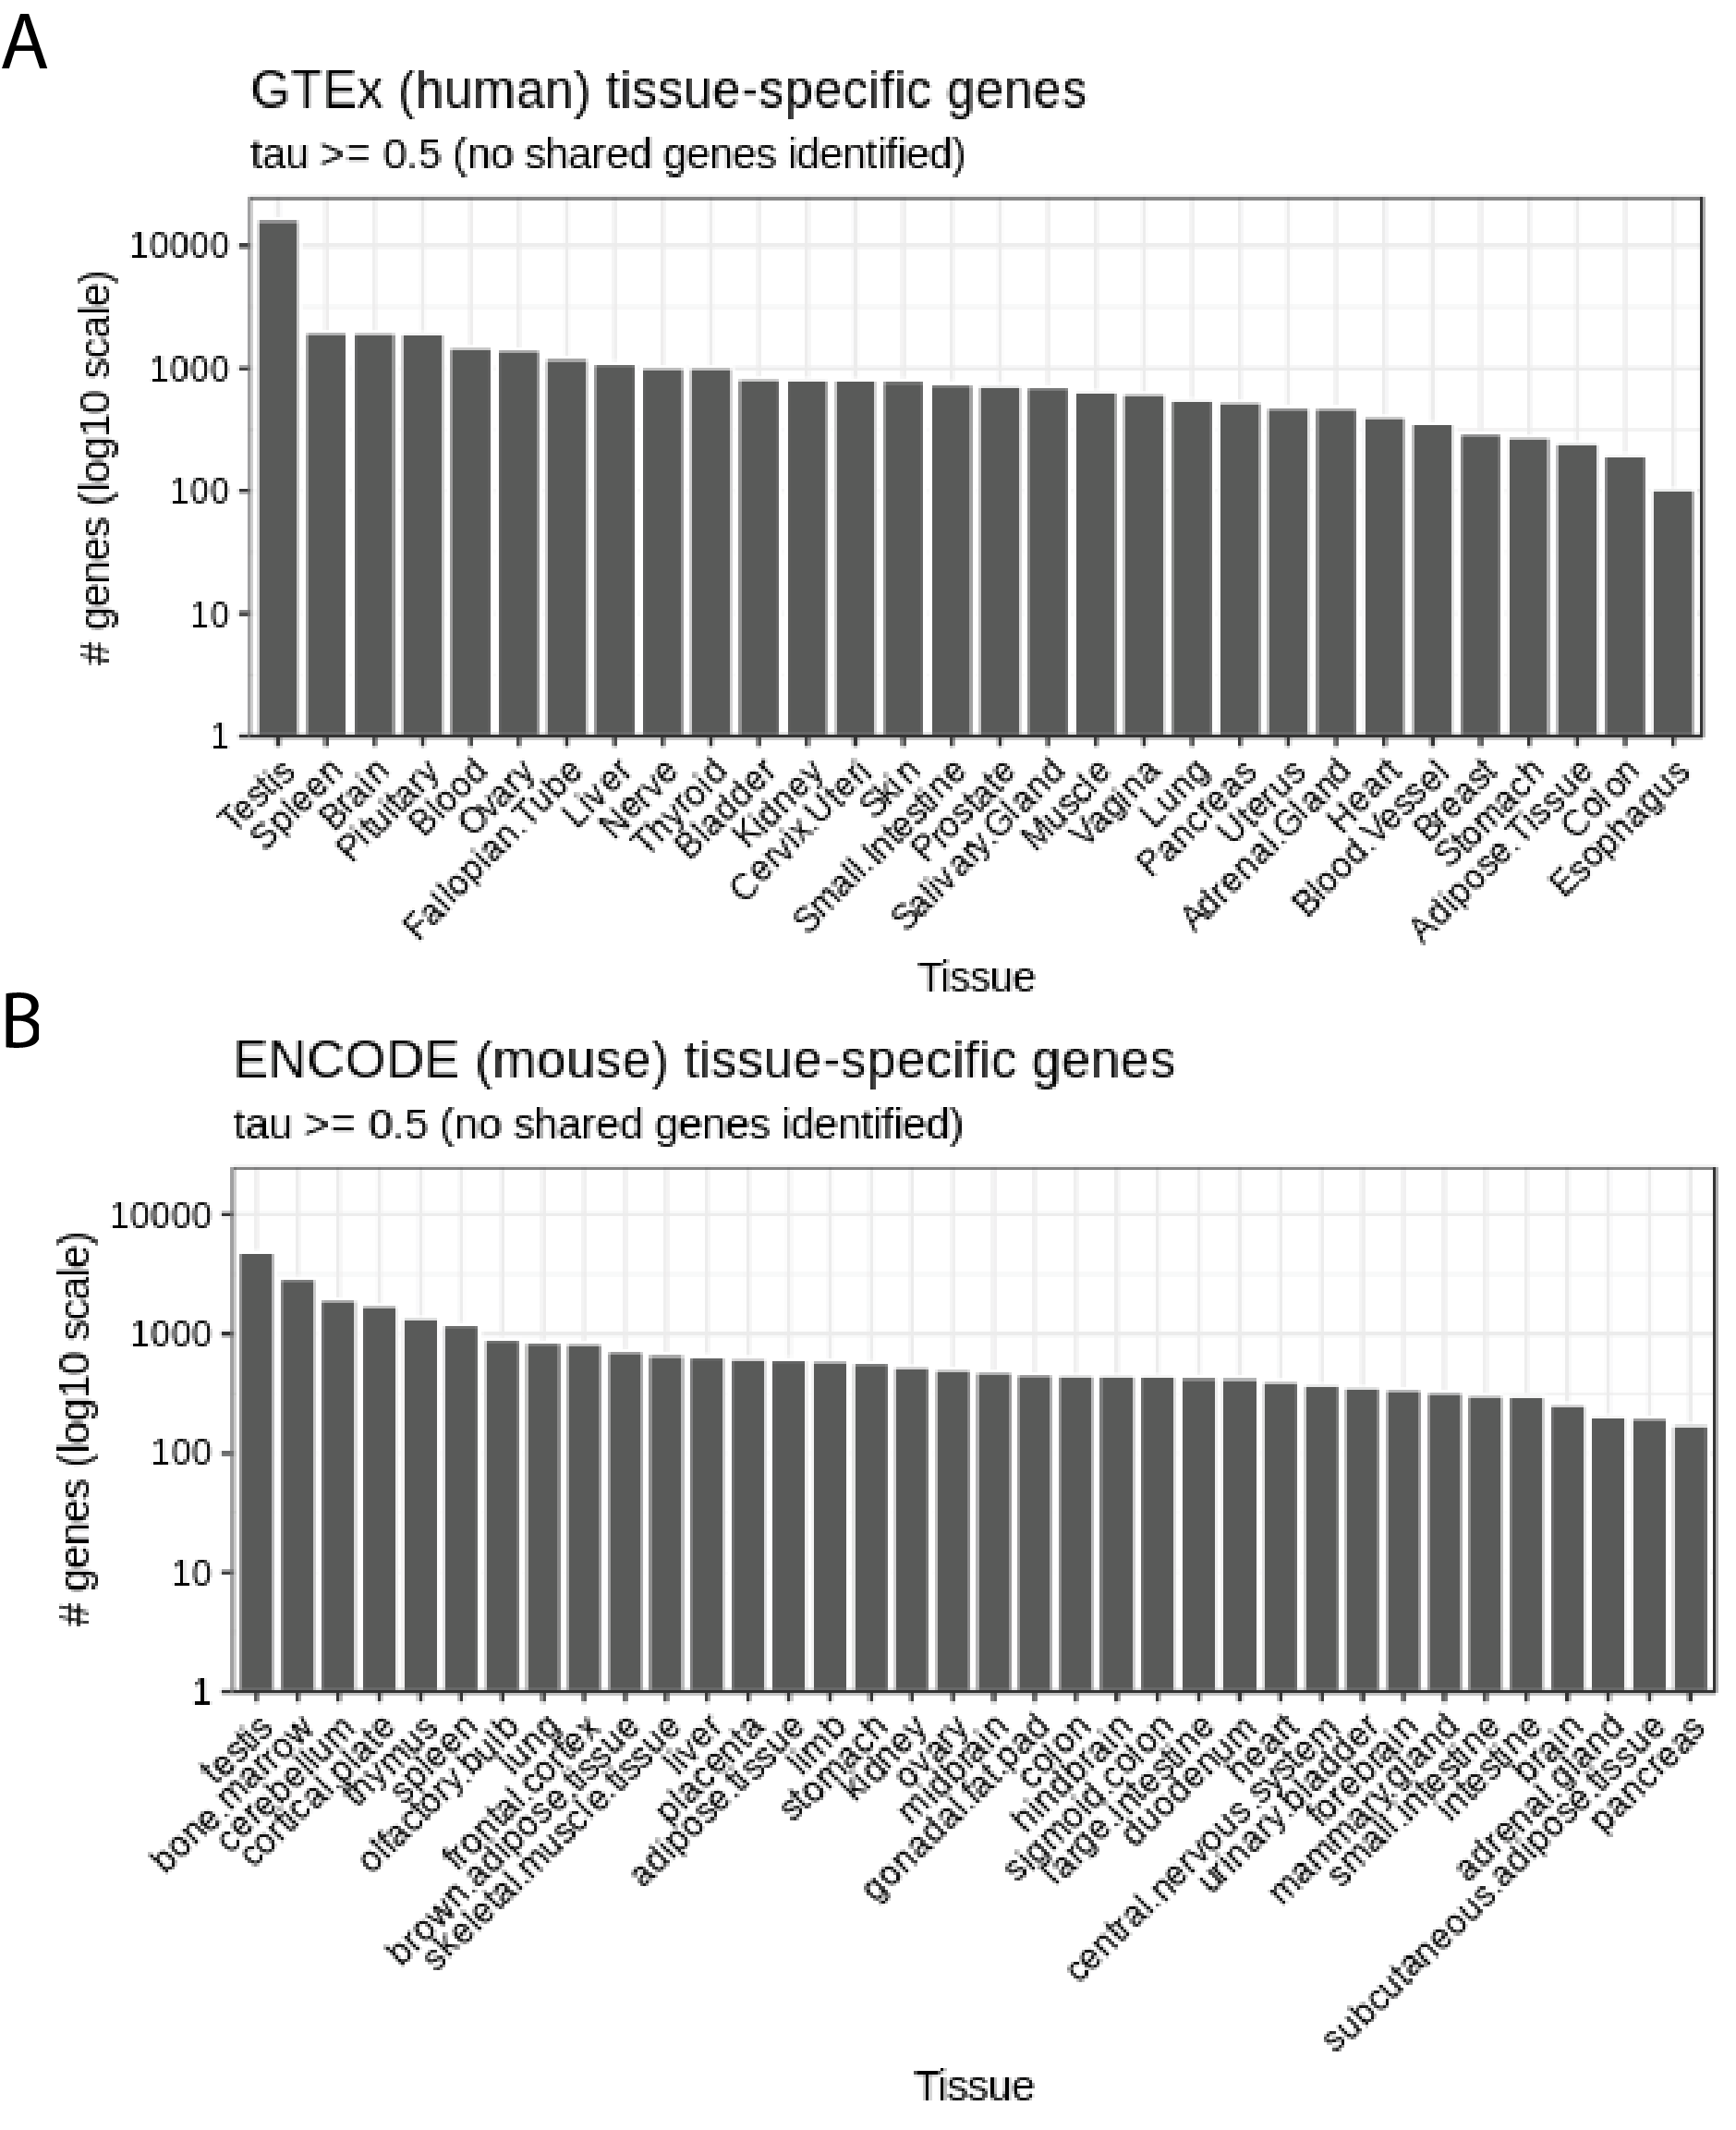
\includegraphics[width=1.0\textwidth]{Appendix3/Figs/appB_uniqueGenesTissue.png} % change word in curlies to change figure
\caption[Number of tissue-specific genes determined per tissue for mouse and human]{\textbf{Number of tissue-specific genes determined per tissue for human (A) and mouse (B))}\newline Tissue specific genes were determined by calculating tau (see Section~\ref{section4.4_genelists}) and keeping only those with a value greater than 0.5. No genes shared between tissues were found.}
\label{fig:appB_uniquegenes}
\end{figure}


\begin{figure}[hb!] 
\centering    
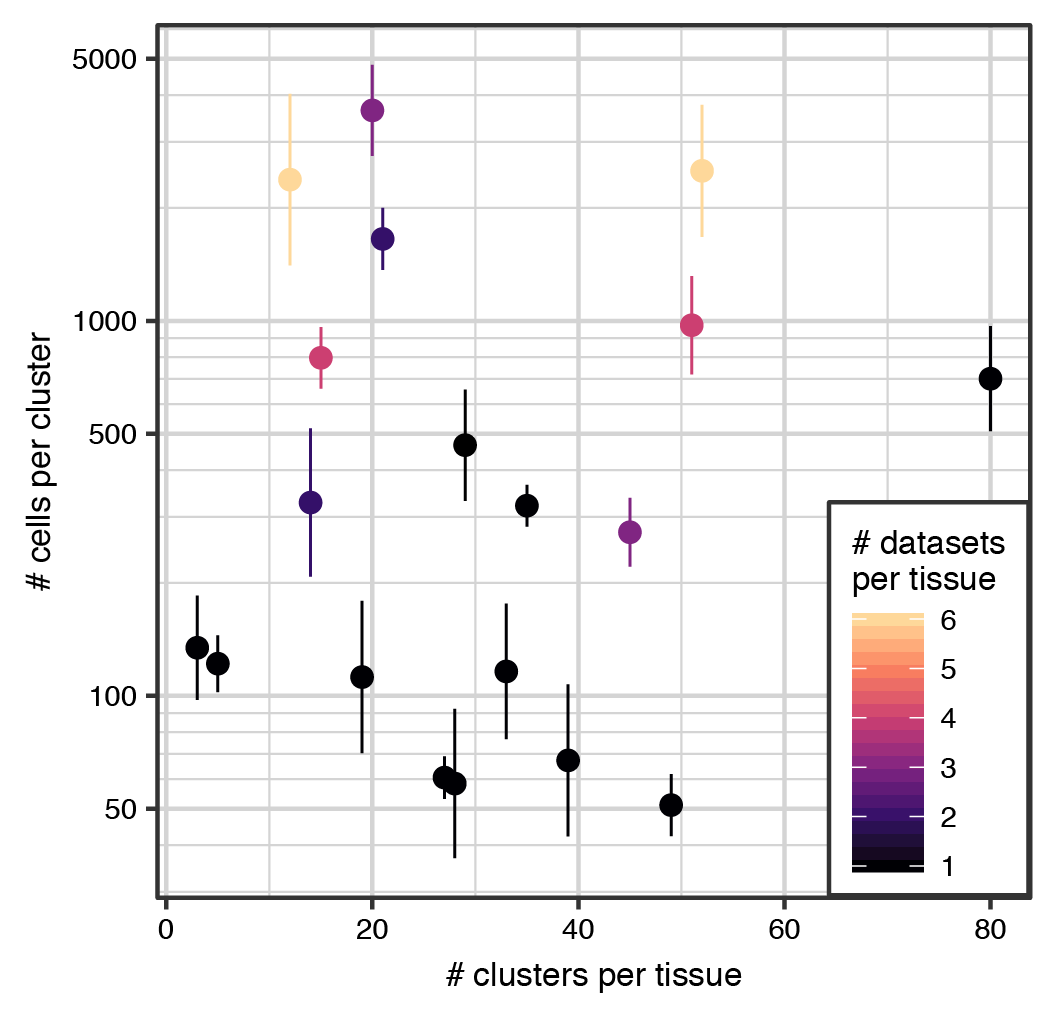
\includegraphics[scale=1.1]{Appendix3/Figs/tissue_cluster_dataset_numbers_HumanAtlas.png} % change word in curlies to change figure
\caption[Relating number of per-tissue clusters and number of cells]{\textbf{Relating number of per-tissue clusters and number of cells (Related to Figure~\ref{fig:chap3_HA}A)}\newline Scatter plot showing the variation of number of clusters per tissue with the number of cells, as well as number of datasets collected for each tissue (colour).}
\label{fig:appB_clustnumbs}
\end{figure}


\begin{figure}[ht!] 
\centering
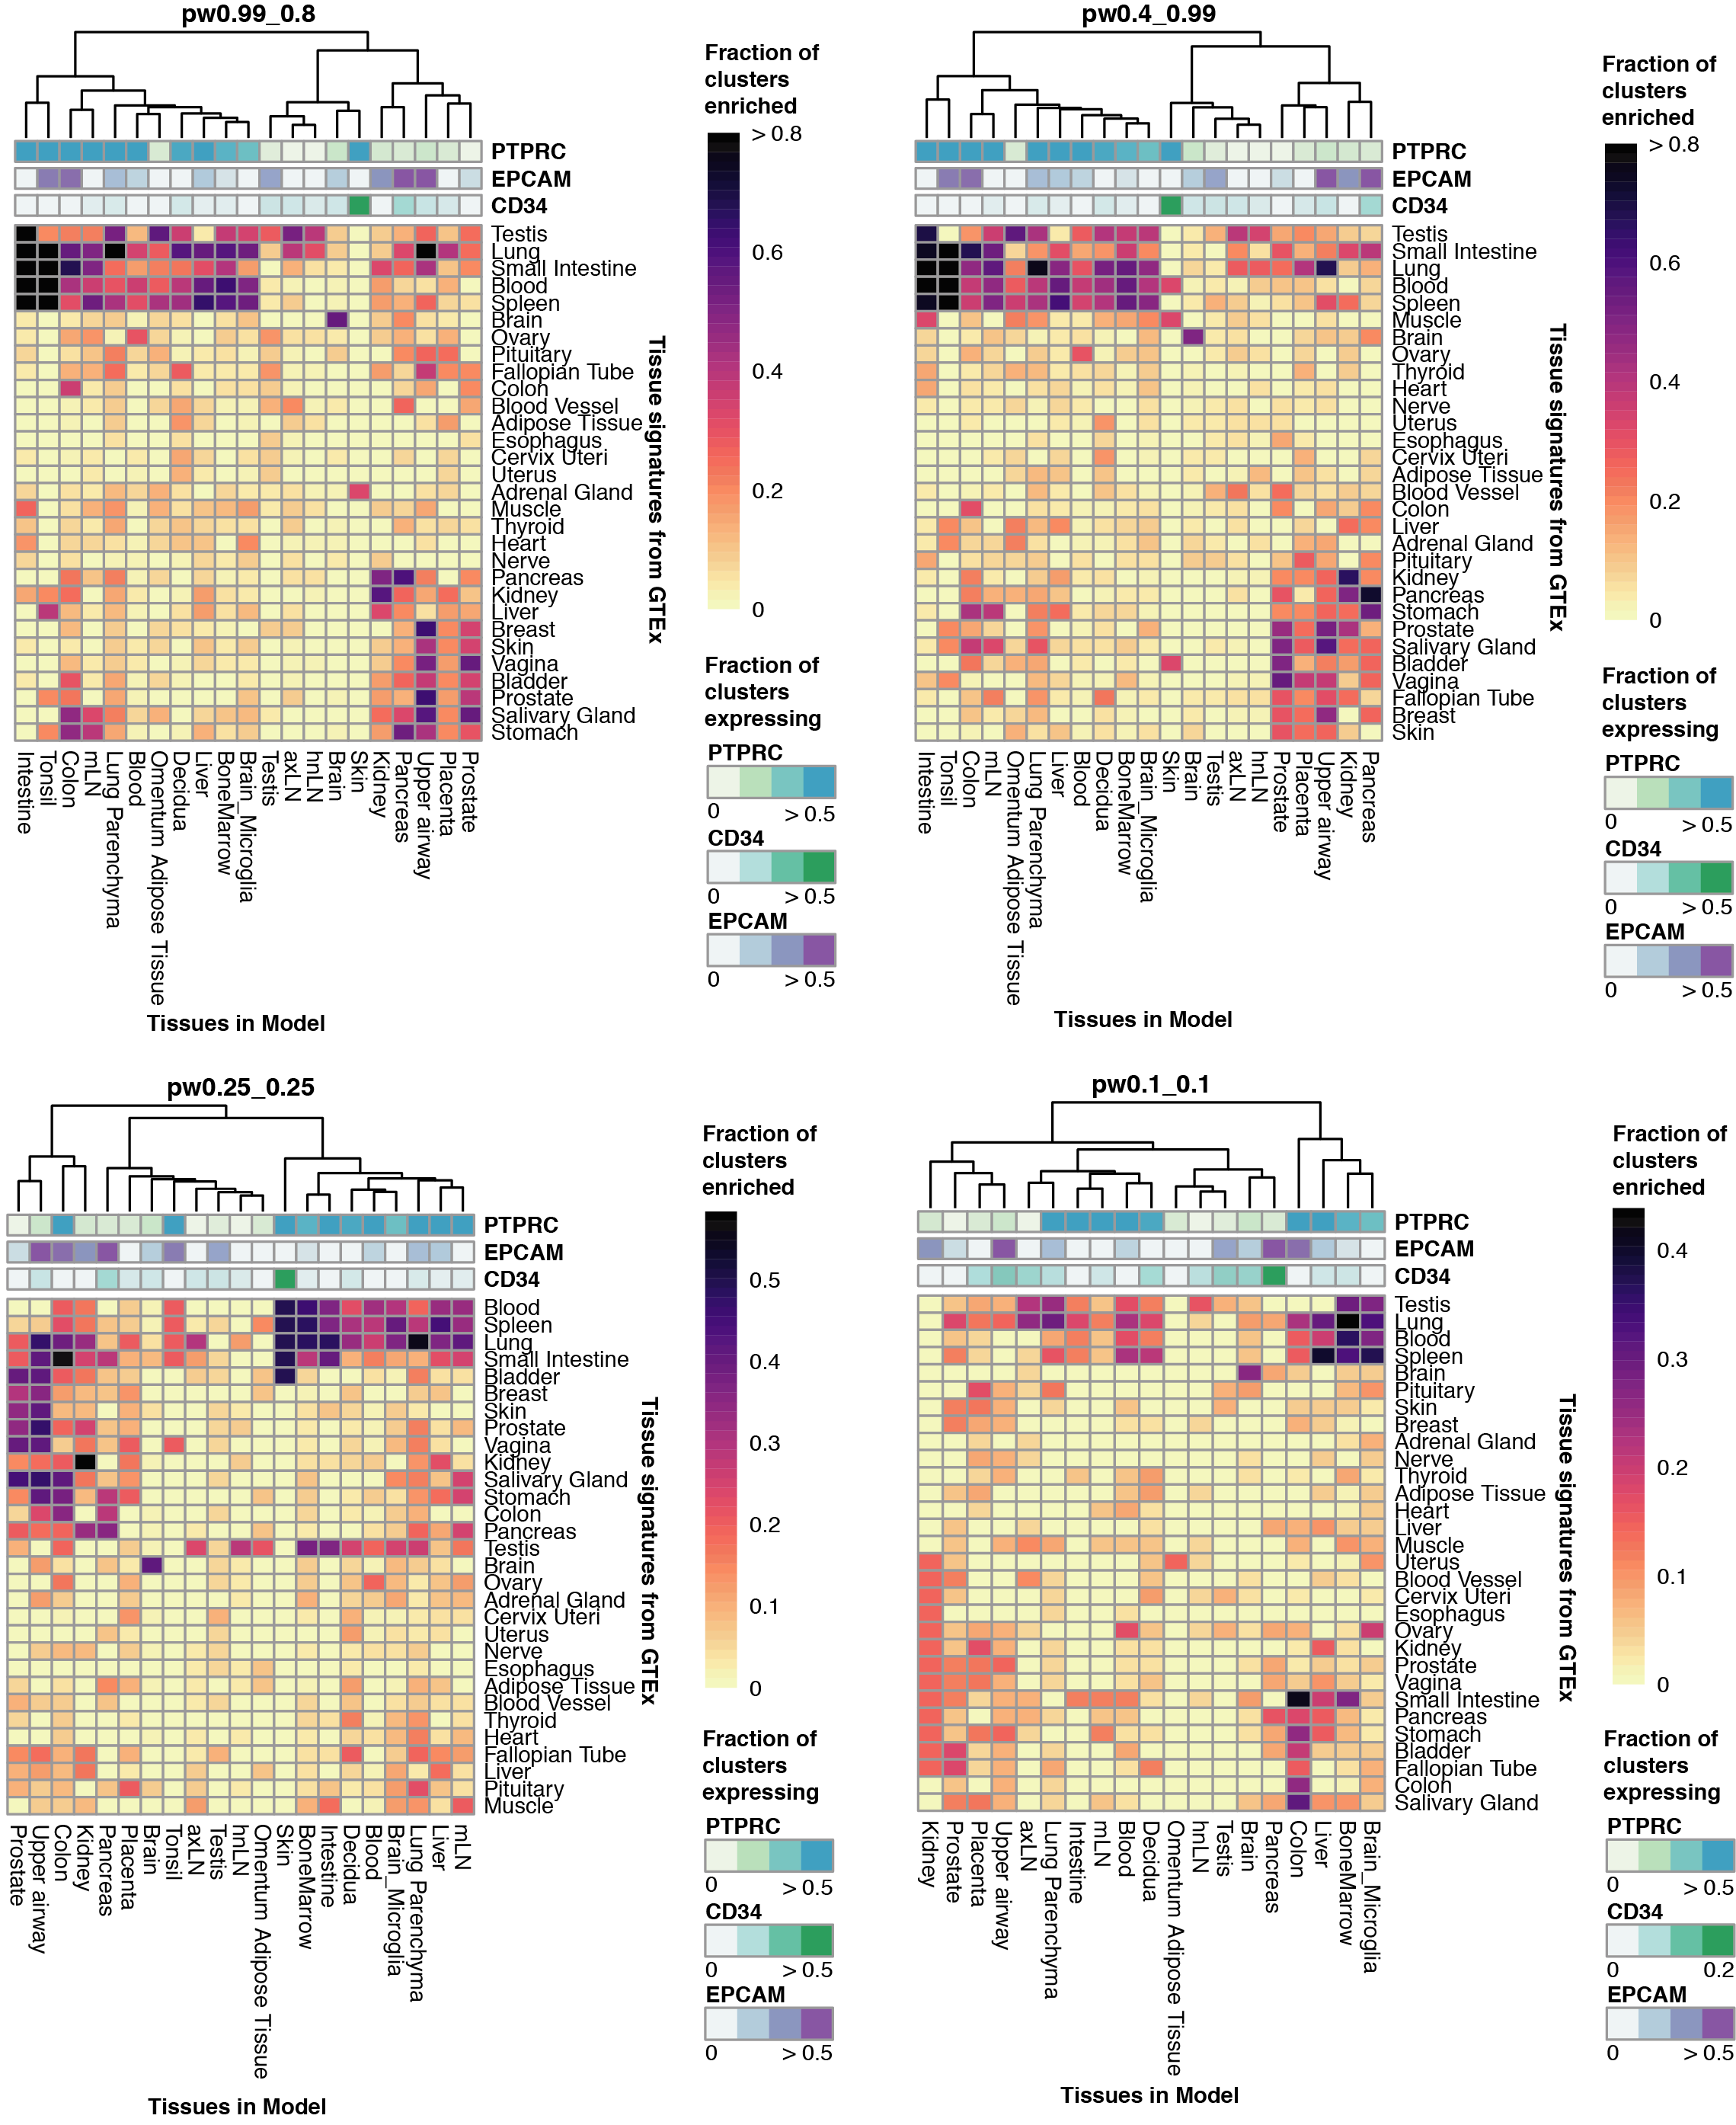
\includegraphics[scale=0.77]{Appendix3/Figs/appB_tissueGSEA.png} % change word in curlies to change figure
\caption[Enrichment of tissue gene modules in other \textit{CellTypist} models]{\textbf{Enrichment of tissue gene modules in other \textit{CellTypist} models (Related to Figure~\ref{fig:chap4_tiss})}\newline Heatmaps showing the fraction of clusters in each tissue (x-axis) with an enrichment for tissue-specific gene programmes (y-axis) determined from GTEx data. Each heatmap represents a different set of clusters per tissue, resulting from using different parameters in the \textit{CellTypist} pipeline. Plot for thr1 = 0.99, thr2 = 0.8 is identical to Figure~\ref{fig:chap4_tiss}B.}
\label{fig:appB_tissGSEA}
\end{figure}


\begin{figure}[ht!] 
\centering
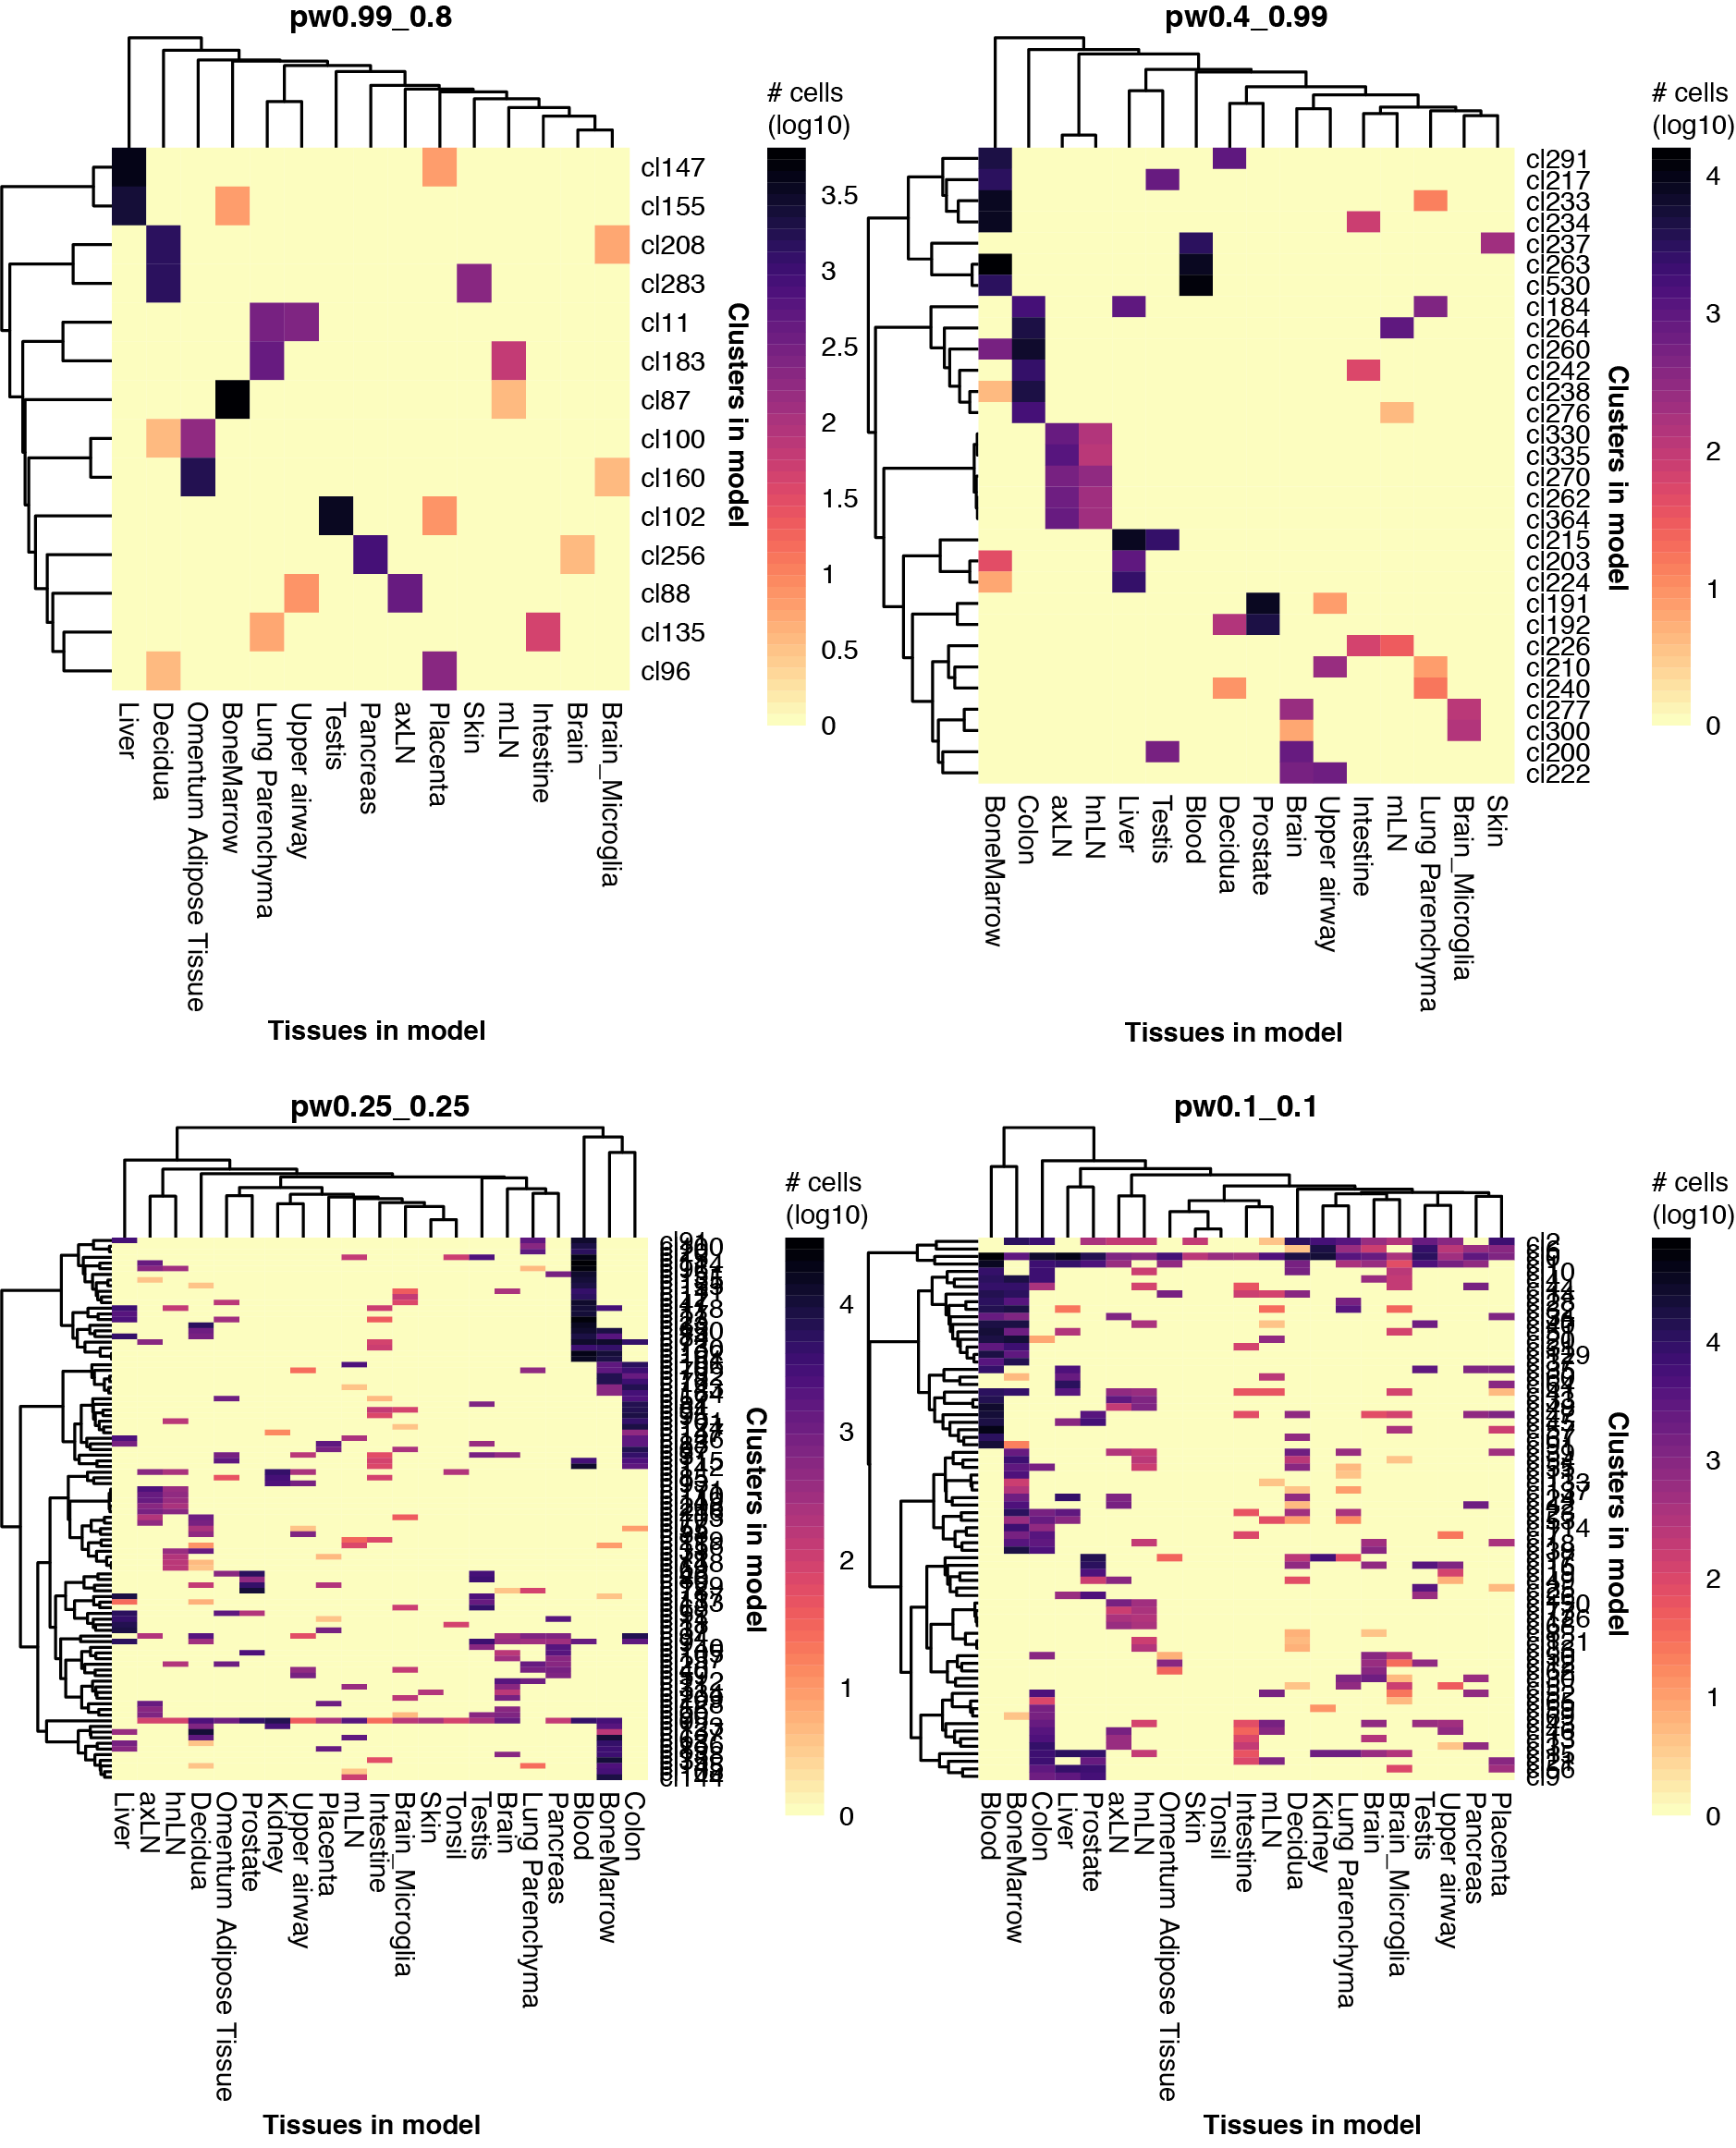
\includegraphics[width=1.0\textwidth]{Appendix3/Figs/appB_tissue_clustrelations_HumanAtlas.png} % change word in curlies to change figure
\caption[Clusters merged across tissues in the different models]{\textbf{Clusters merged across tissues in the different models (Related to Figure~\ref{fig:chap4_tiss})}\newline Heatmaps showing the number of cells contributed by each tissue into cross-tissue clusters for each model.}
\label{fig:appC_tissrel}
\end{figure}


\begin{figure}[ht!] 
\centering
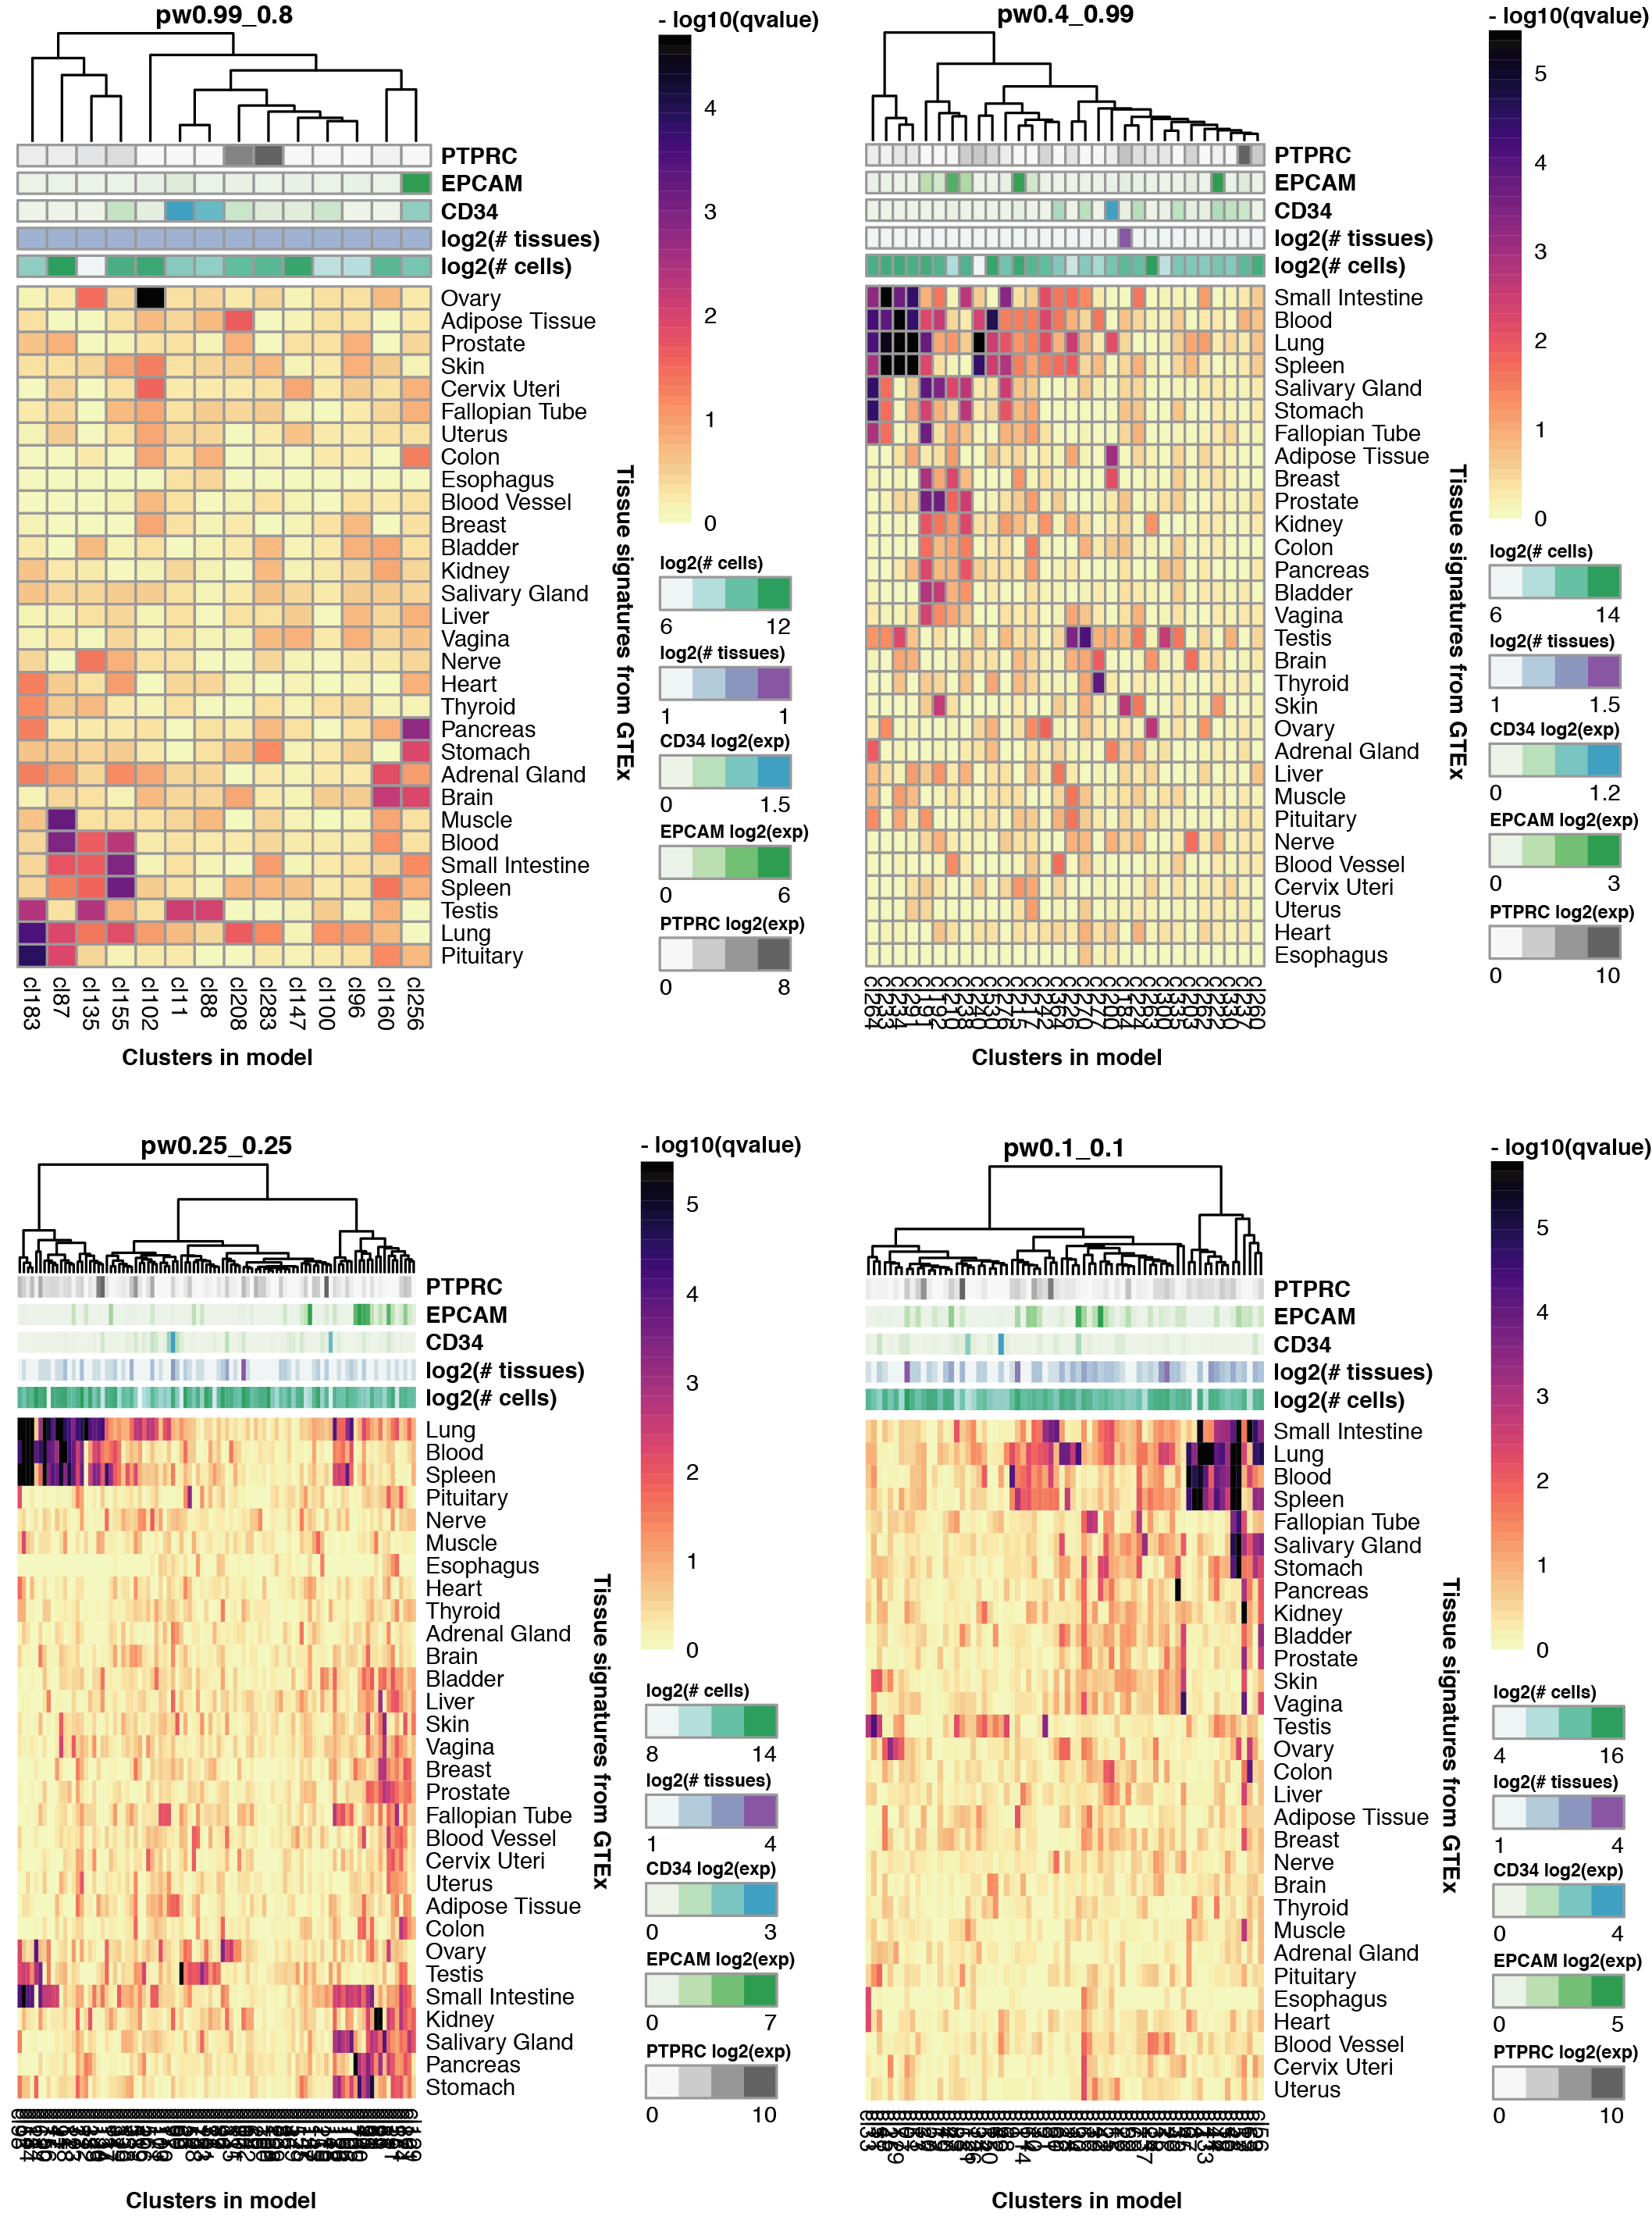
\includegraphics[scale=0.77]{Appendix3/Figs/appB_clmGSEA.png} % change word in curlies to change figure
\caption[Enrichment of tissue gene modules in merged clusters of different \textit{CellTypist} models]{\textbf{Enrichment of tissue gene modules in merged clusters of different \textit{CellTypist} models (Related to Figure~\ref{fig:chap4_tiss})}\newline Heatmaps showing the -log10(q-value) of each merged cluster (x-axis) for the enrichment of tissue-specific gene programmes (y-axis) in their top 500 genes output by the model. Each heatmap represents a different set of merged clusters, resulting from using different parameters in the \textit{CellTypist} pipeline.}
\label{fig:appB_clmGSEA}
\end{figure}


\begin{figure}[ht!] 
\centering
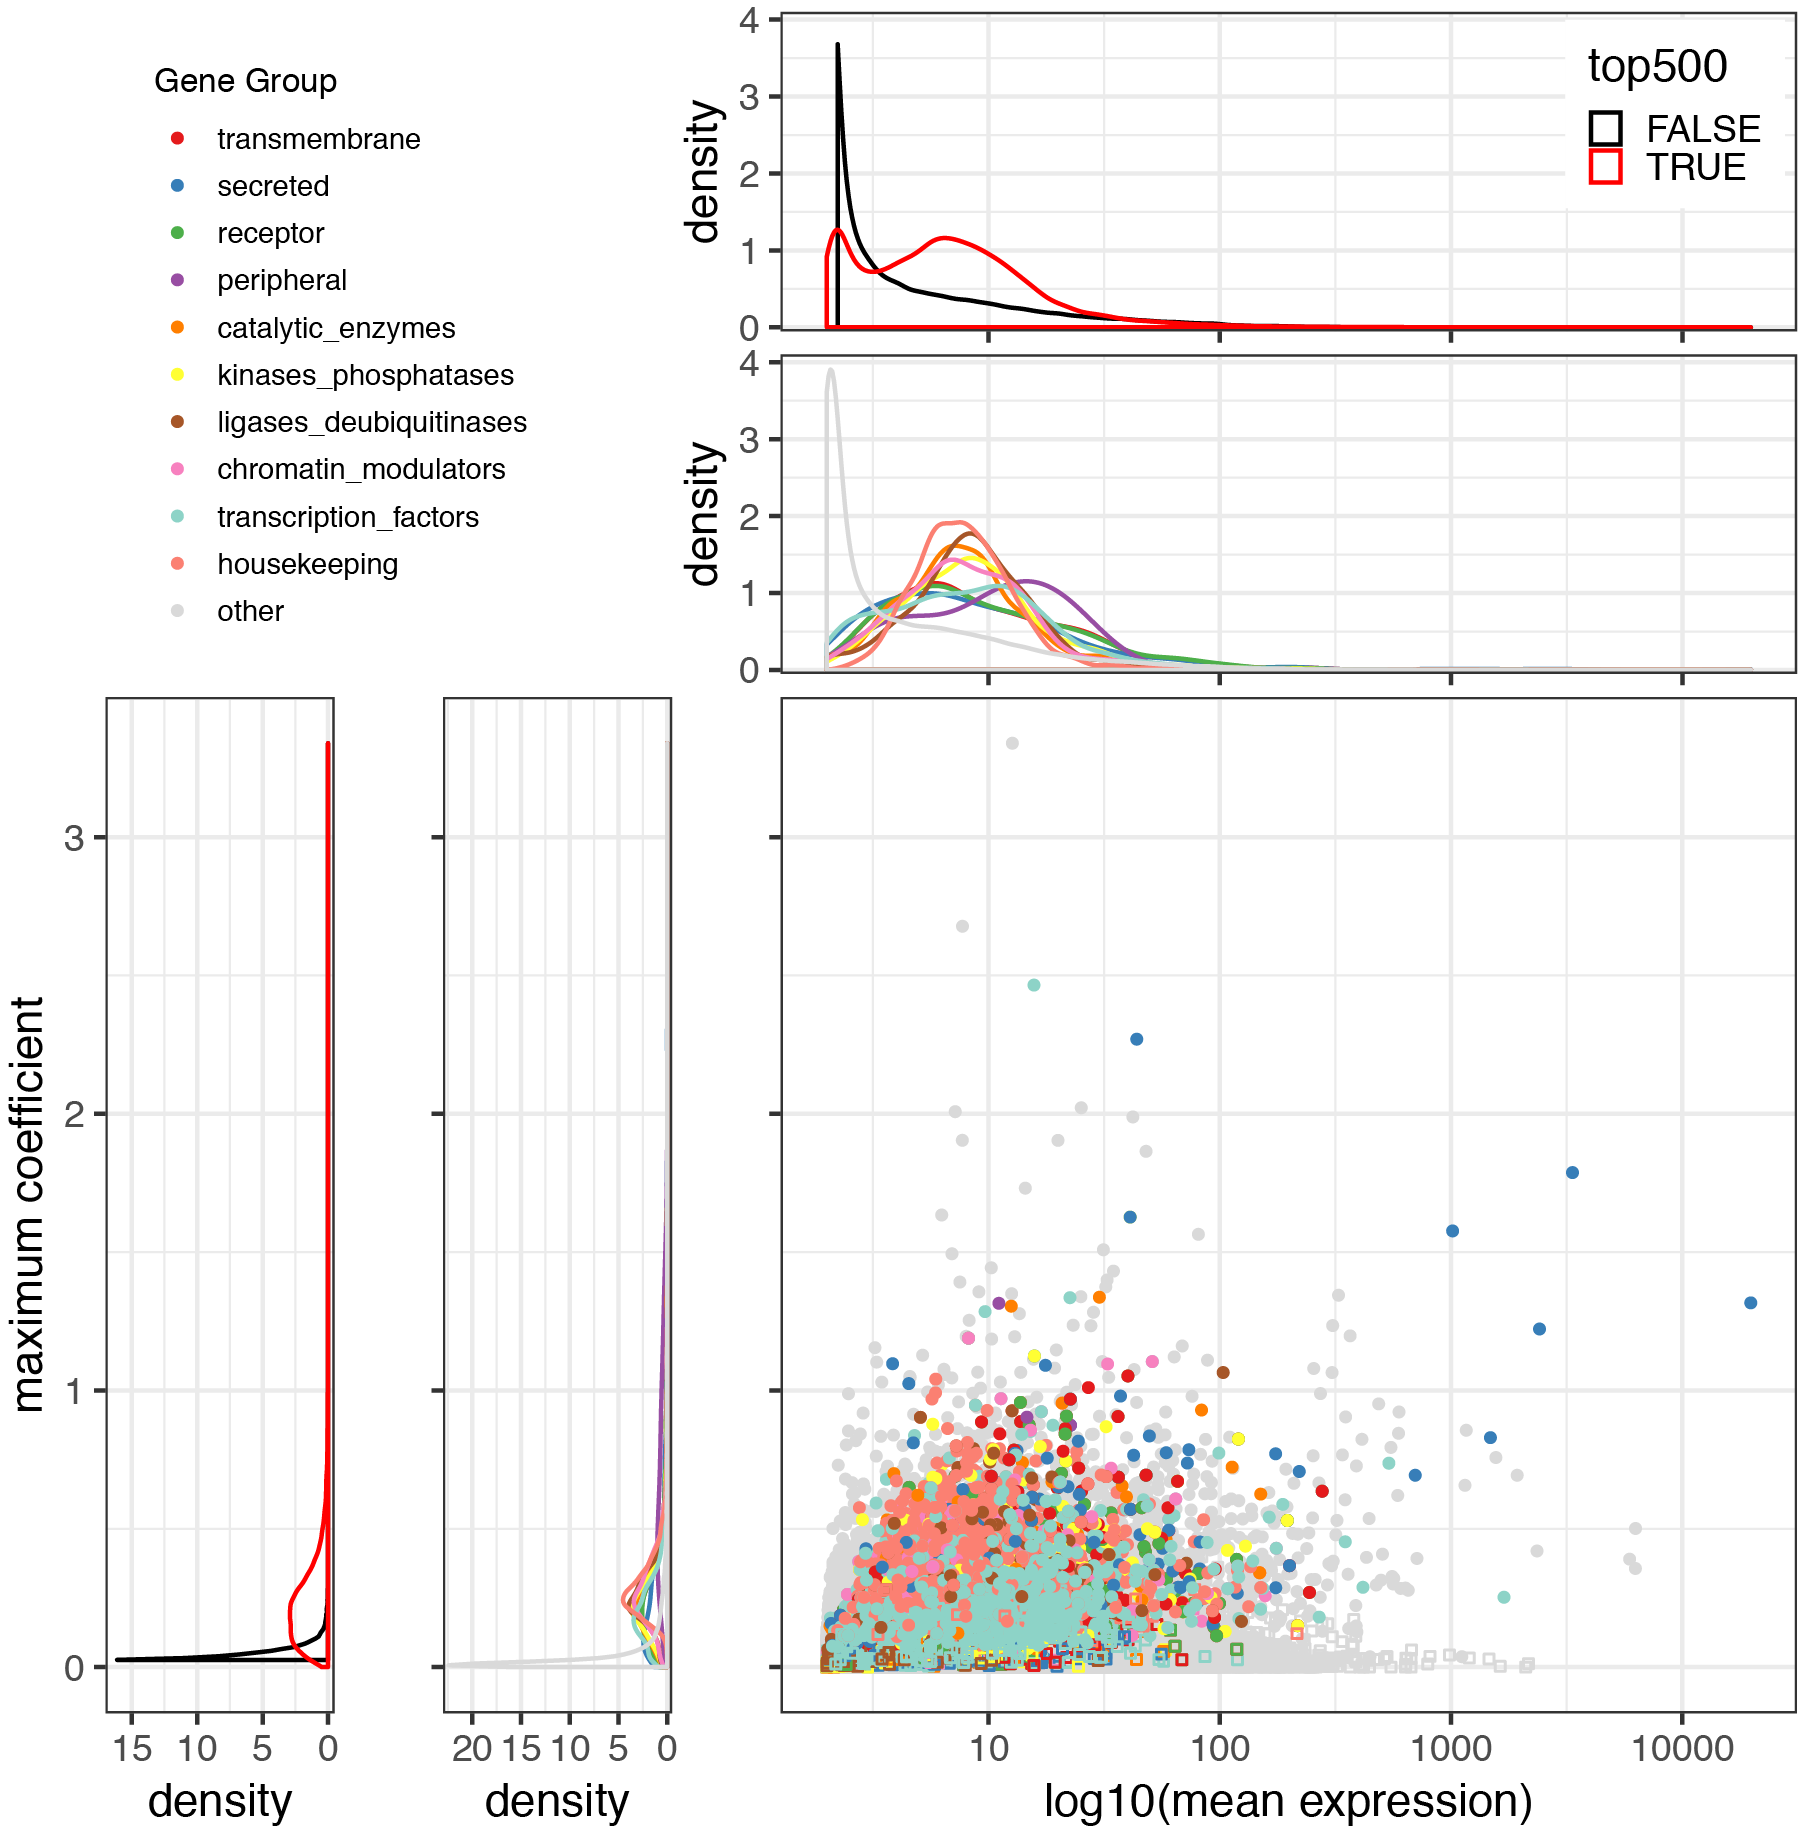
\includegraphics[scale=0.9]{Appendix3/Figs/gene_coeff_exp_HumanAtlas.png} % change word in curlies to change figure
\caption[Correlation between gene expression and importance in the human \textit{CellTypist} model]{\textbf{Correlation between gene expression and importance in the human \textit{CellTypist} model (Related to Figure~\ref{fig:chap4_genetypes})}\newline Scatterplot shows the relationship between mean expression across all cells and the maximum coefficient for each gene across all labels. Density plots show distribution of gene groups, and distribution of genes included in the top 500 coefficients of any label, along the mean expression (top) or maximum coefficient (left) range. Spearman correlation coefficient = 0.56, p-value < 0.01.}
\label{fig:appB_human_coeff_exp}
\end{figure}


\begin{figure}[ht!] 
\centering
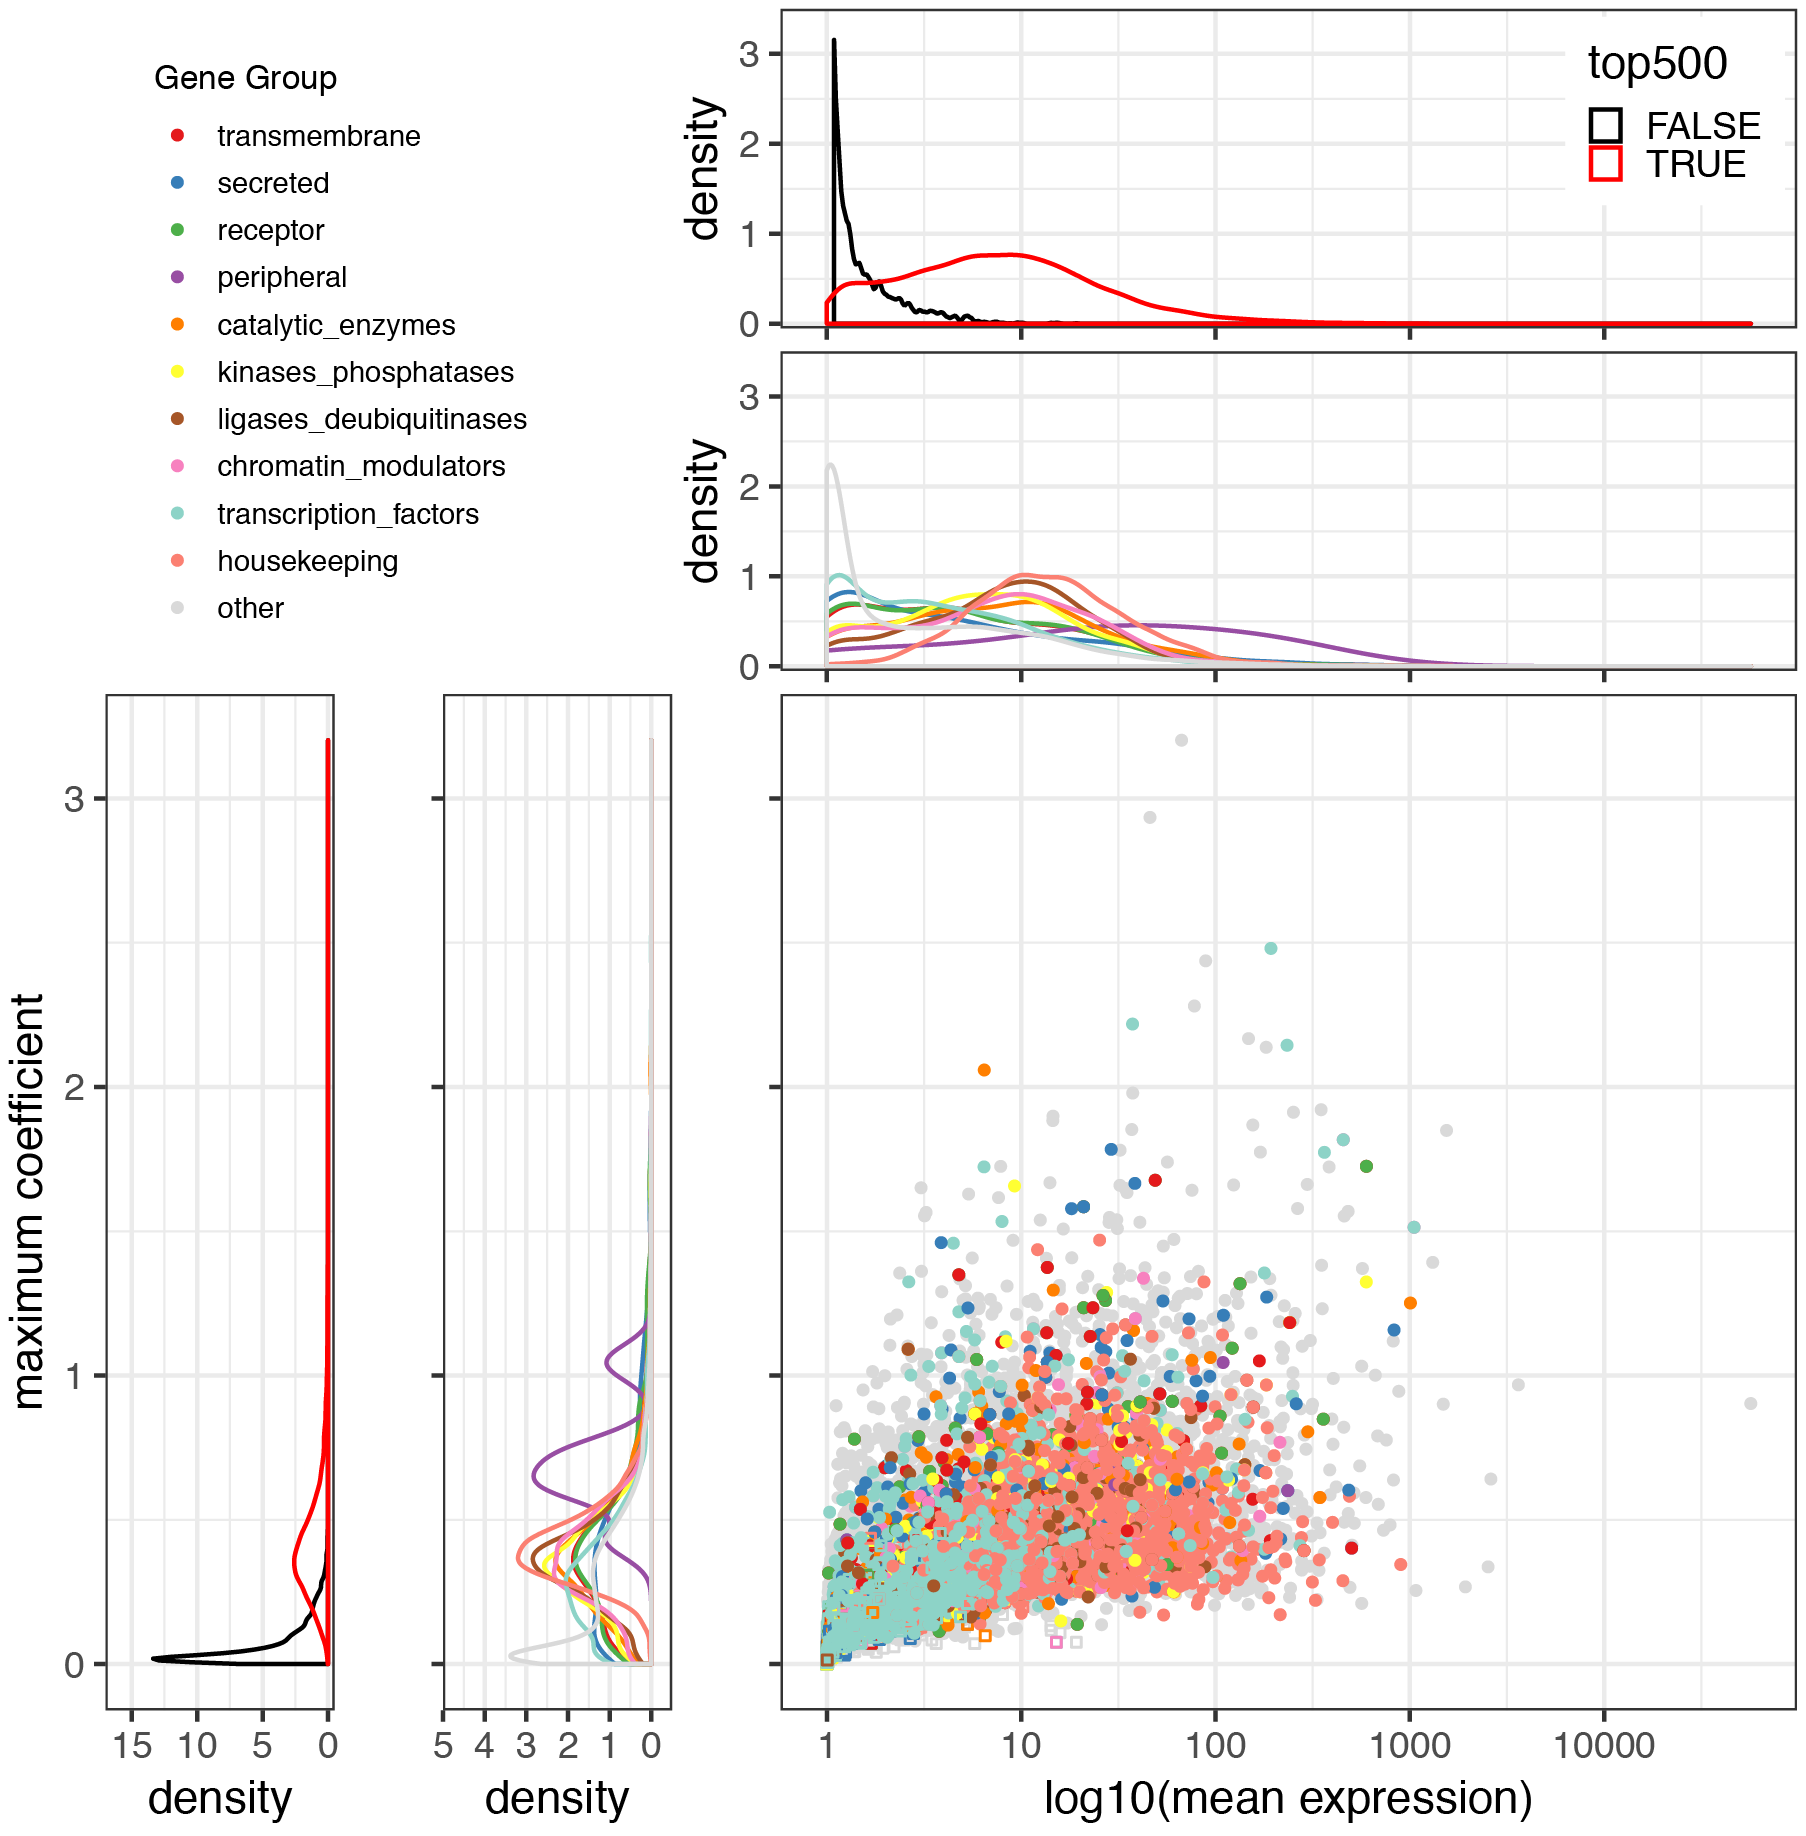
\includegraphics[scale=0.9]{Appendix3/Figs/gene_coeff_exp_TabulaMuris.png} % change word in curlies to change figure
\caption[Correlation between gene expression and importance in the \textit{Tabula Muris} \textit{CellTypist} model]{\textbf{Correlation between gene expression and importance in the \textit{Tabula Muris} \textit{CellTypist} model (Related to Figure~\ref{fig:chap4_genetypes_mouse})}\newline Scatterplot shows the relationship between mean expression across all cells and the maximum coefficient for each gene across all labels. Density plots show distribution of gene groups, and distribution of genes included in the top 500 coefficients of any label, along the mean expression (top) or maximum coefficient (left) range. Spearman correlation coefficient = 0.86, p-value < 0.01.}
\label{fig:appB_mouse_coeff_exp}
\end{figure}


\begin{figure}[ht!] 
\centering
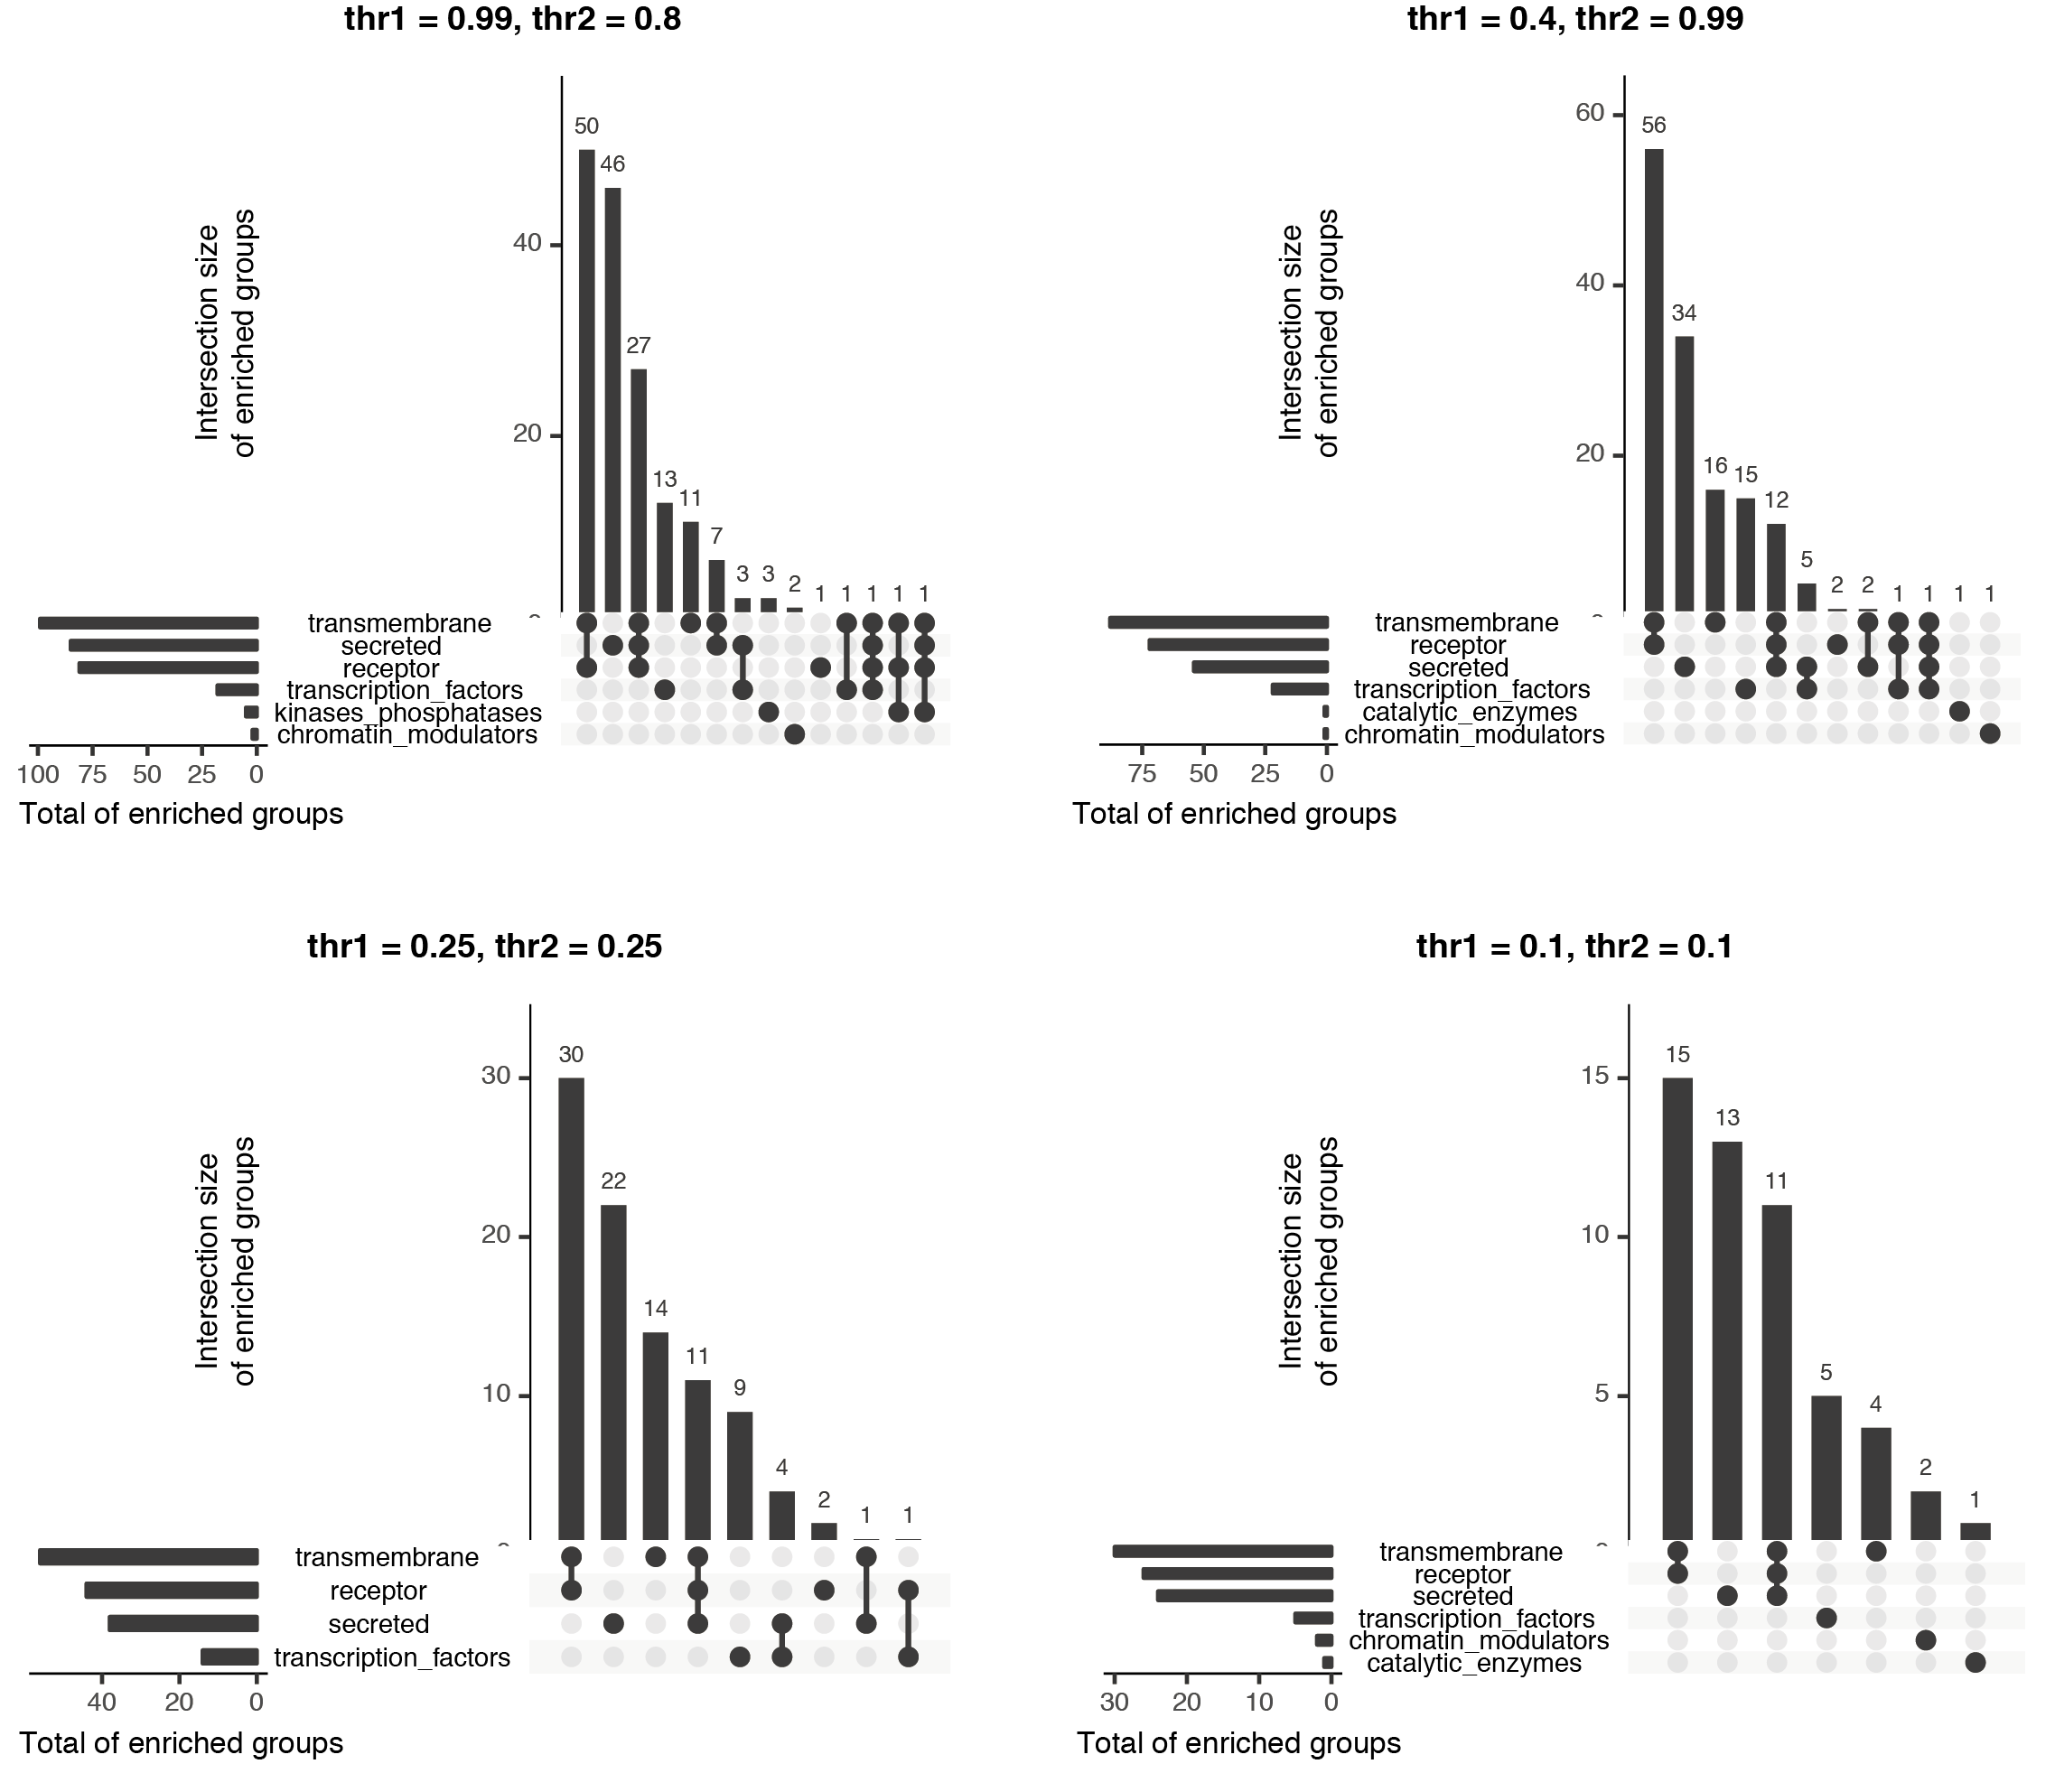
\includegraphics[scale=0.79]{Appendix3/Figs/appB_upset.png} % change word in curlies to change figure
\caption[Gene upset plots of different \textit{CellTypist} models]{\textbf{Gene upset plots of different \textit{CellTypist} models (Related to Figure~\ref{fig:chap4_genetypes})}\newline Upset plots counting the number of clusters enriched for a specific group of genes in each model. The gene groups tested were "transcription factors", "transmembrane", "secreted", "receptors", "membrane peripheral proteins", "kinases and phosphatases", "chromatin modulators", "catalytic enzymes", "housekeeping genes". Only the terms enriched in at least one cluster were shown. The plot for thr1 = 0.99, thr2 = 0.8 is identical to Figure~\ref{fig:chap4_genetypes}B.}
\label{fig:appB_supupset}
\end{figure}


\begin{figure}[pht!] 
\centering
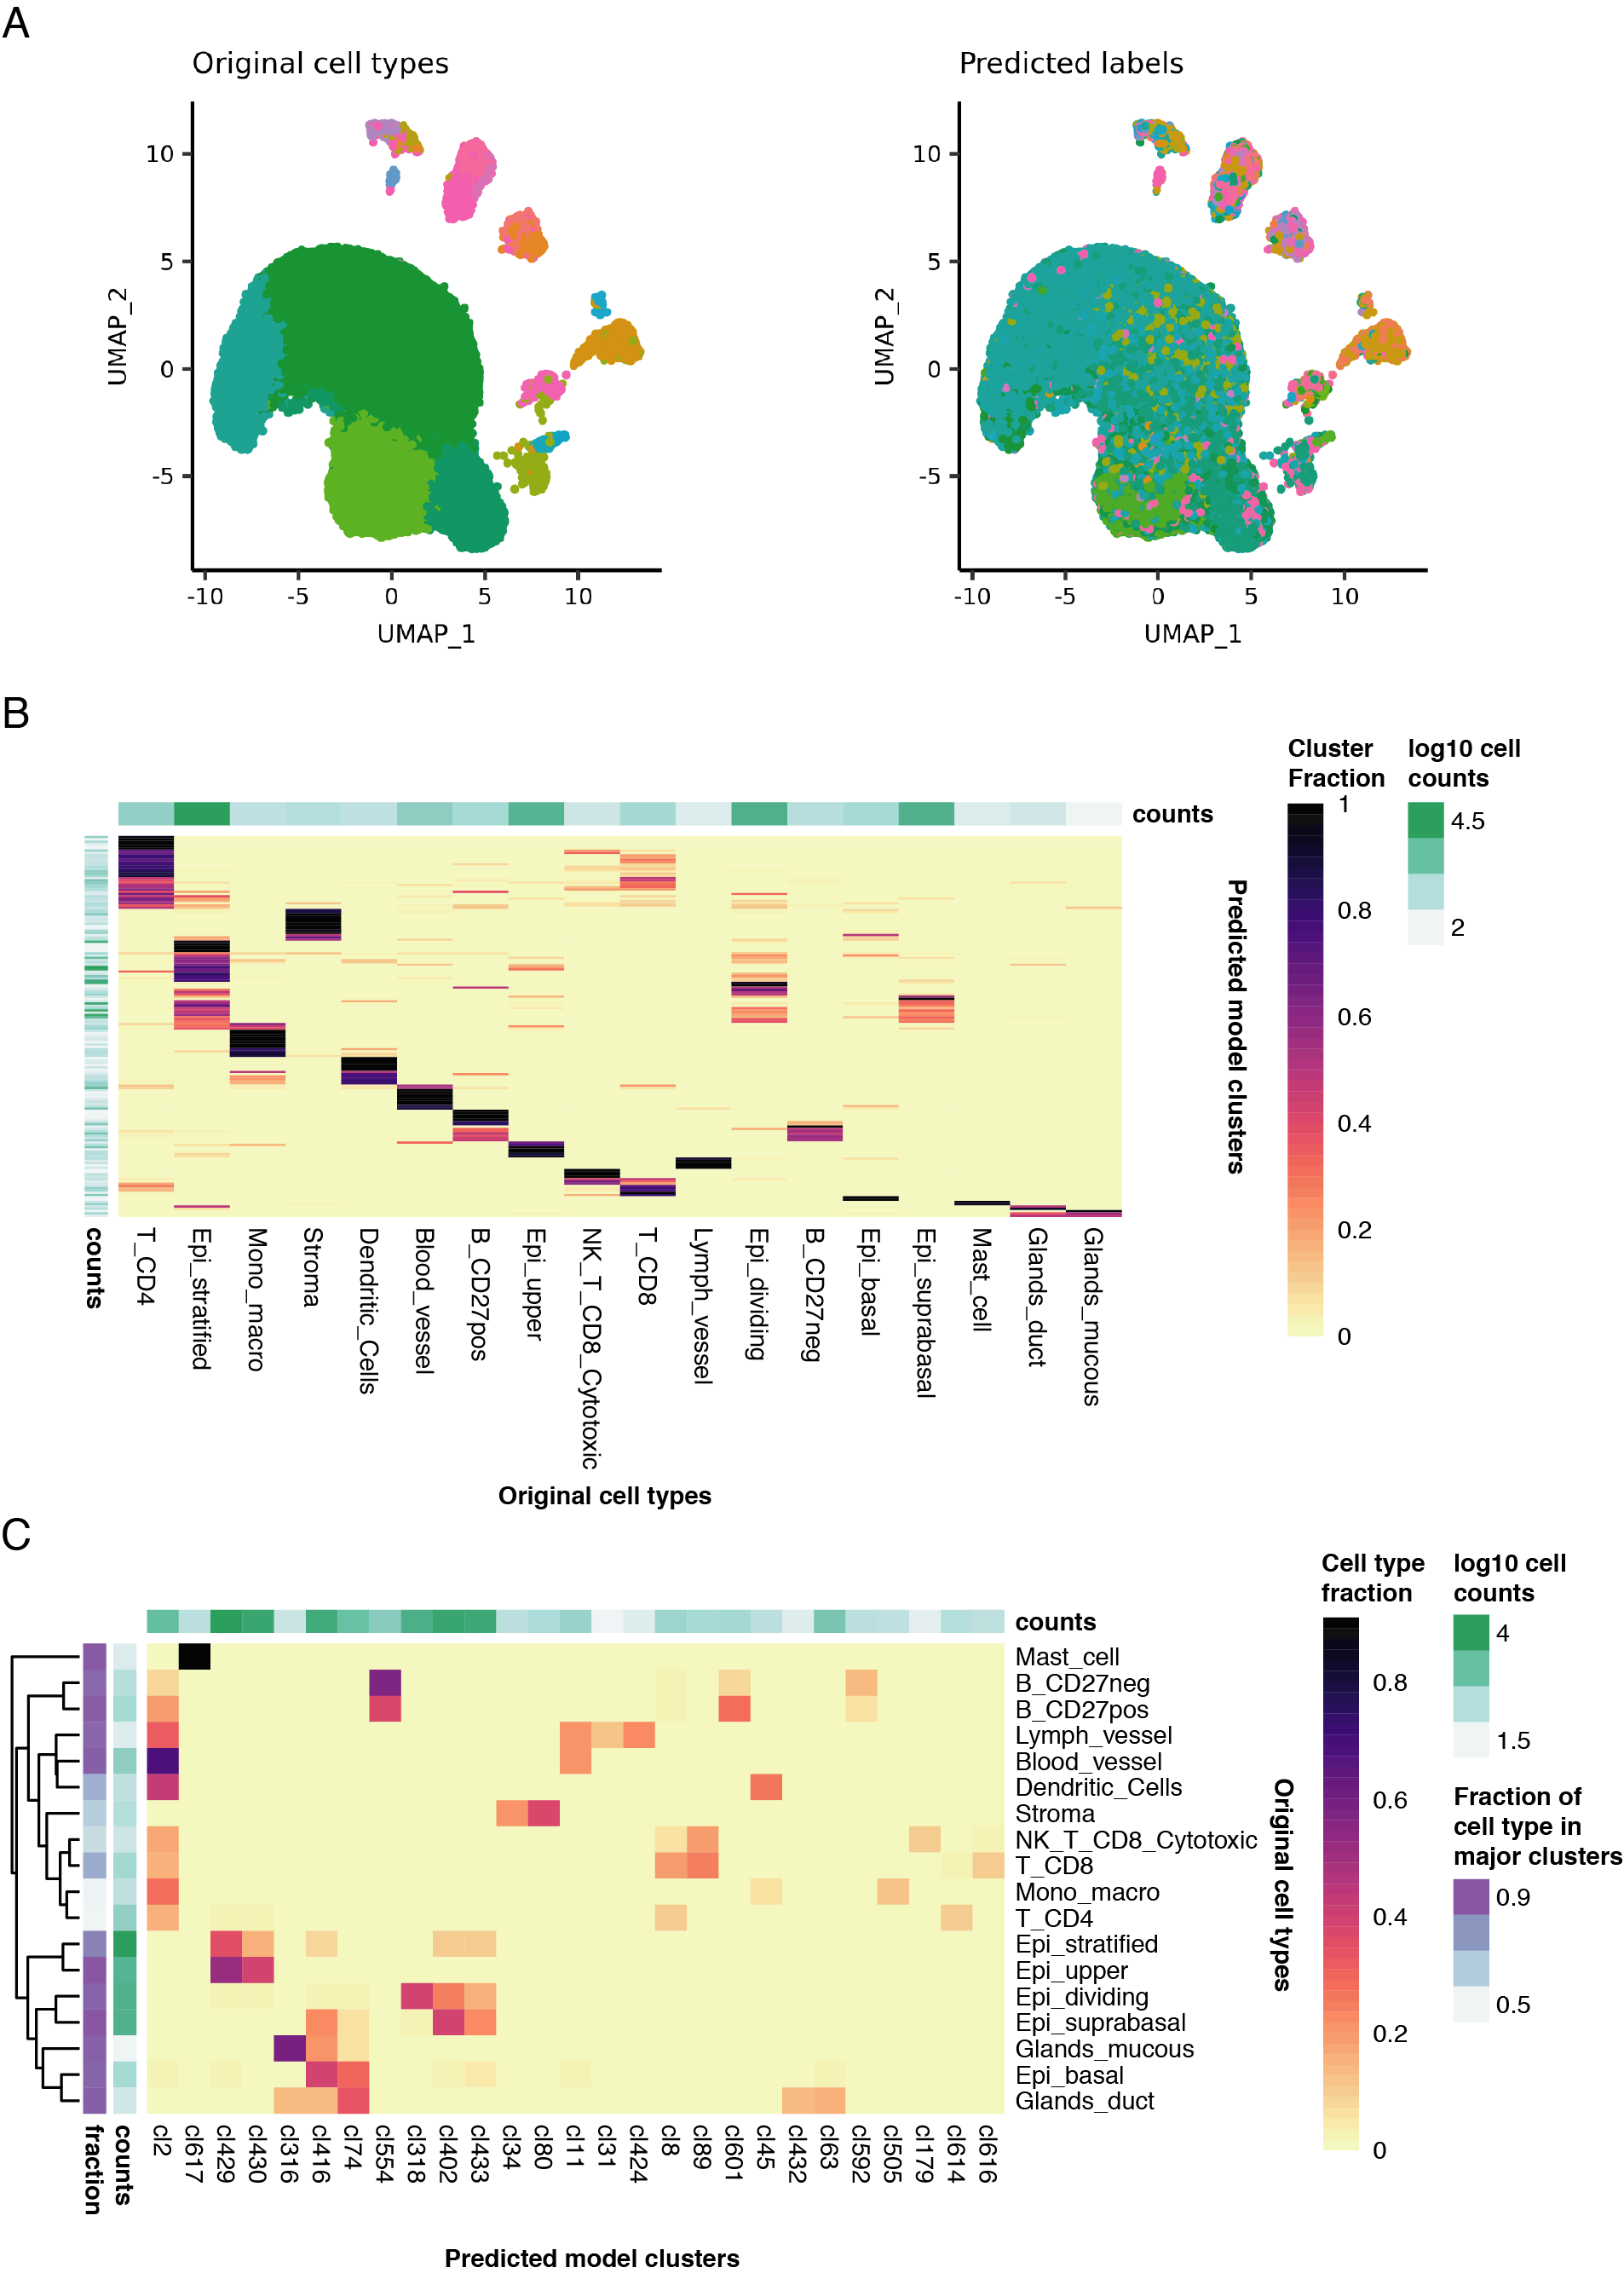
\includegraphics[scale=0.8]{Appendix3/Figs/appB_oes.png} % change word in curlies to change figure
\caption[\textit{CellTypist} predictions for oesophagus data from~\citep{madissoon_lung_2019}]{\textbf{\textit{CellTypist} predictions for oesophagus data from~\citep{madissoon_lung_2019} (Related to Figure~\ref{fig:chap4_preds})}\newline\textbf{(A)} UMAP projections coloured by the original cell type annotations (left) and those predicted by \textit{CellTypist} (right) using thr1 = 0.99 and thr2 = 0.8. \textbf{(B)} Proportion of clusters (rows) matching each annotated cell type (columns). \textbf{(C)} Proportion of annotated cell types (rows) included in each cluster (columns). Only clusters including at least 10\% of a given cell type were included.}
\label{fig:appB_oes}
\end{figure}


\begin{figure}[pht!] 
\centering
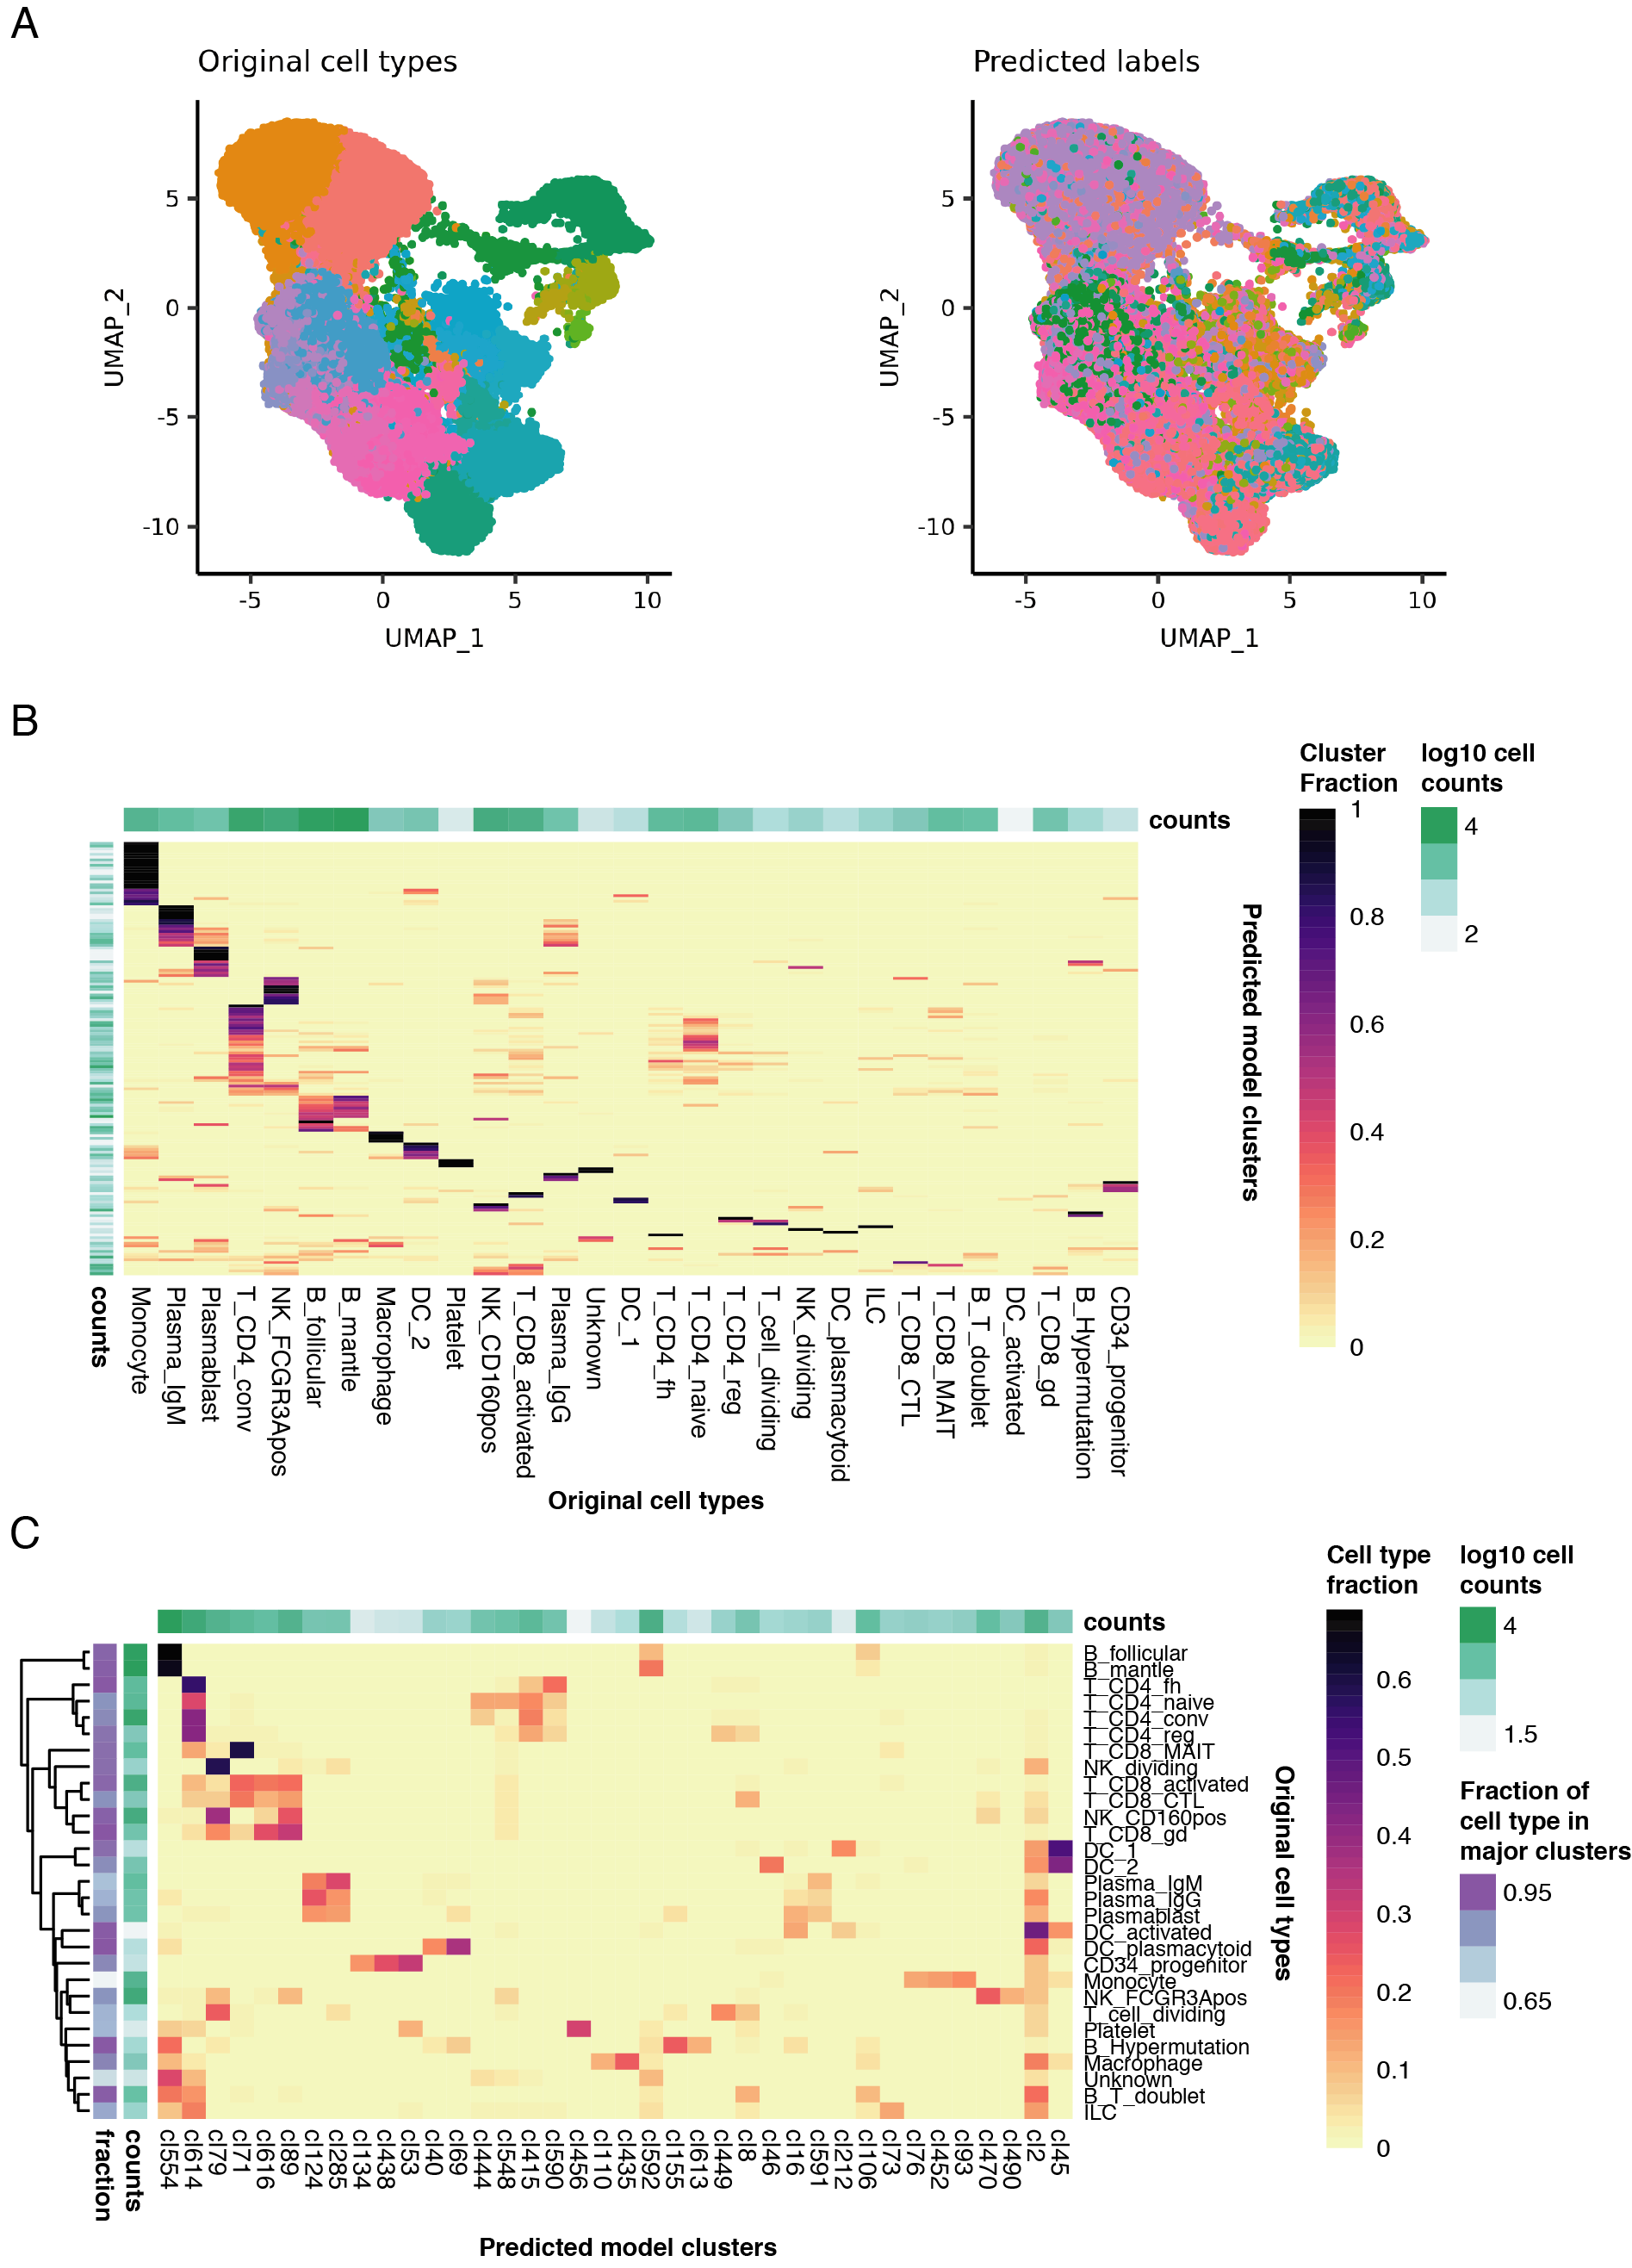
\includegraphics[scale=0.81]{Appendix3/Figs/appB_spleen.png} % change word in curlies to change figure
\caption[\textit{CellTypist} predictions for spleen data from~\citep{madissoon_lung_2019}]{\textbf{\textit{CellTypist} predictions for spleen data from~\citep{madissoon_lung_2019} (Related to Figure~\ref{fig:chap4_preds})}\newline\textbf{(A)} UMAP projections coloured by the original cell type annotations (left) and those predicted by \textit{CellTypist} (right) using thr1 = 0.99 and thr2 = 0.8. \textbf{(B)} Proportion of clusters (rows) matching each annotated cell type (columns). \textbf{(C)} Proportion of annotated cell types (rows) included in each cluster (columns). Only clusters including at least 10\% of a given cell type were included.}
\label{fig:appB_spleen}
\end{figure}


\begin{figure}[pht!] 
\centering
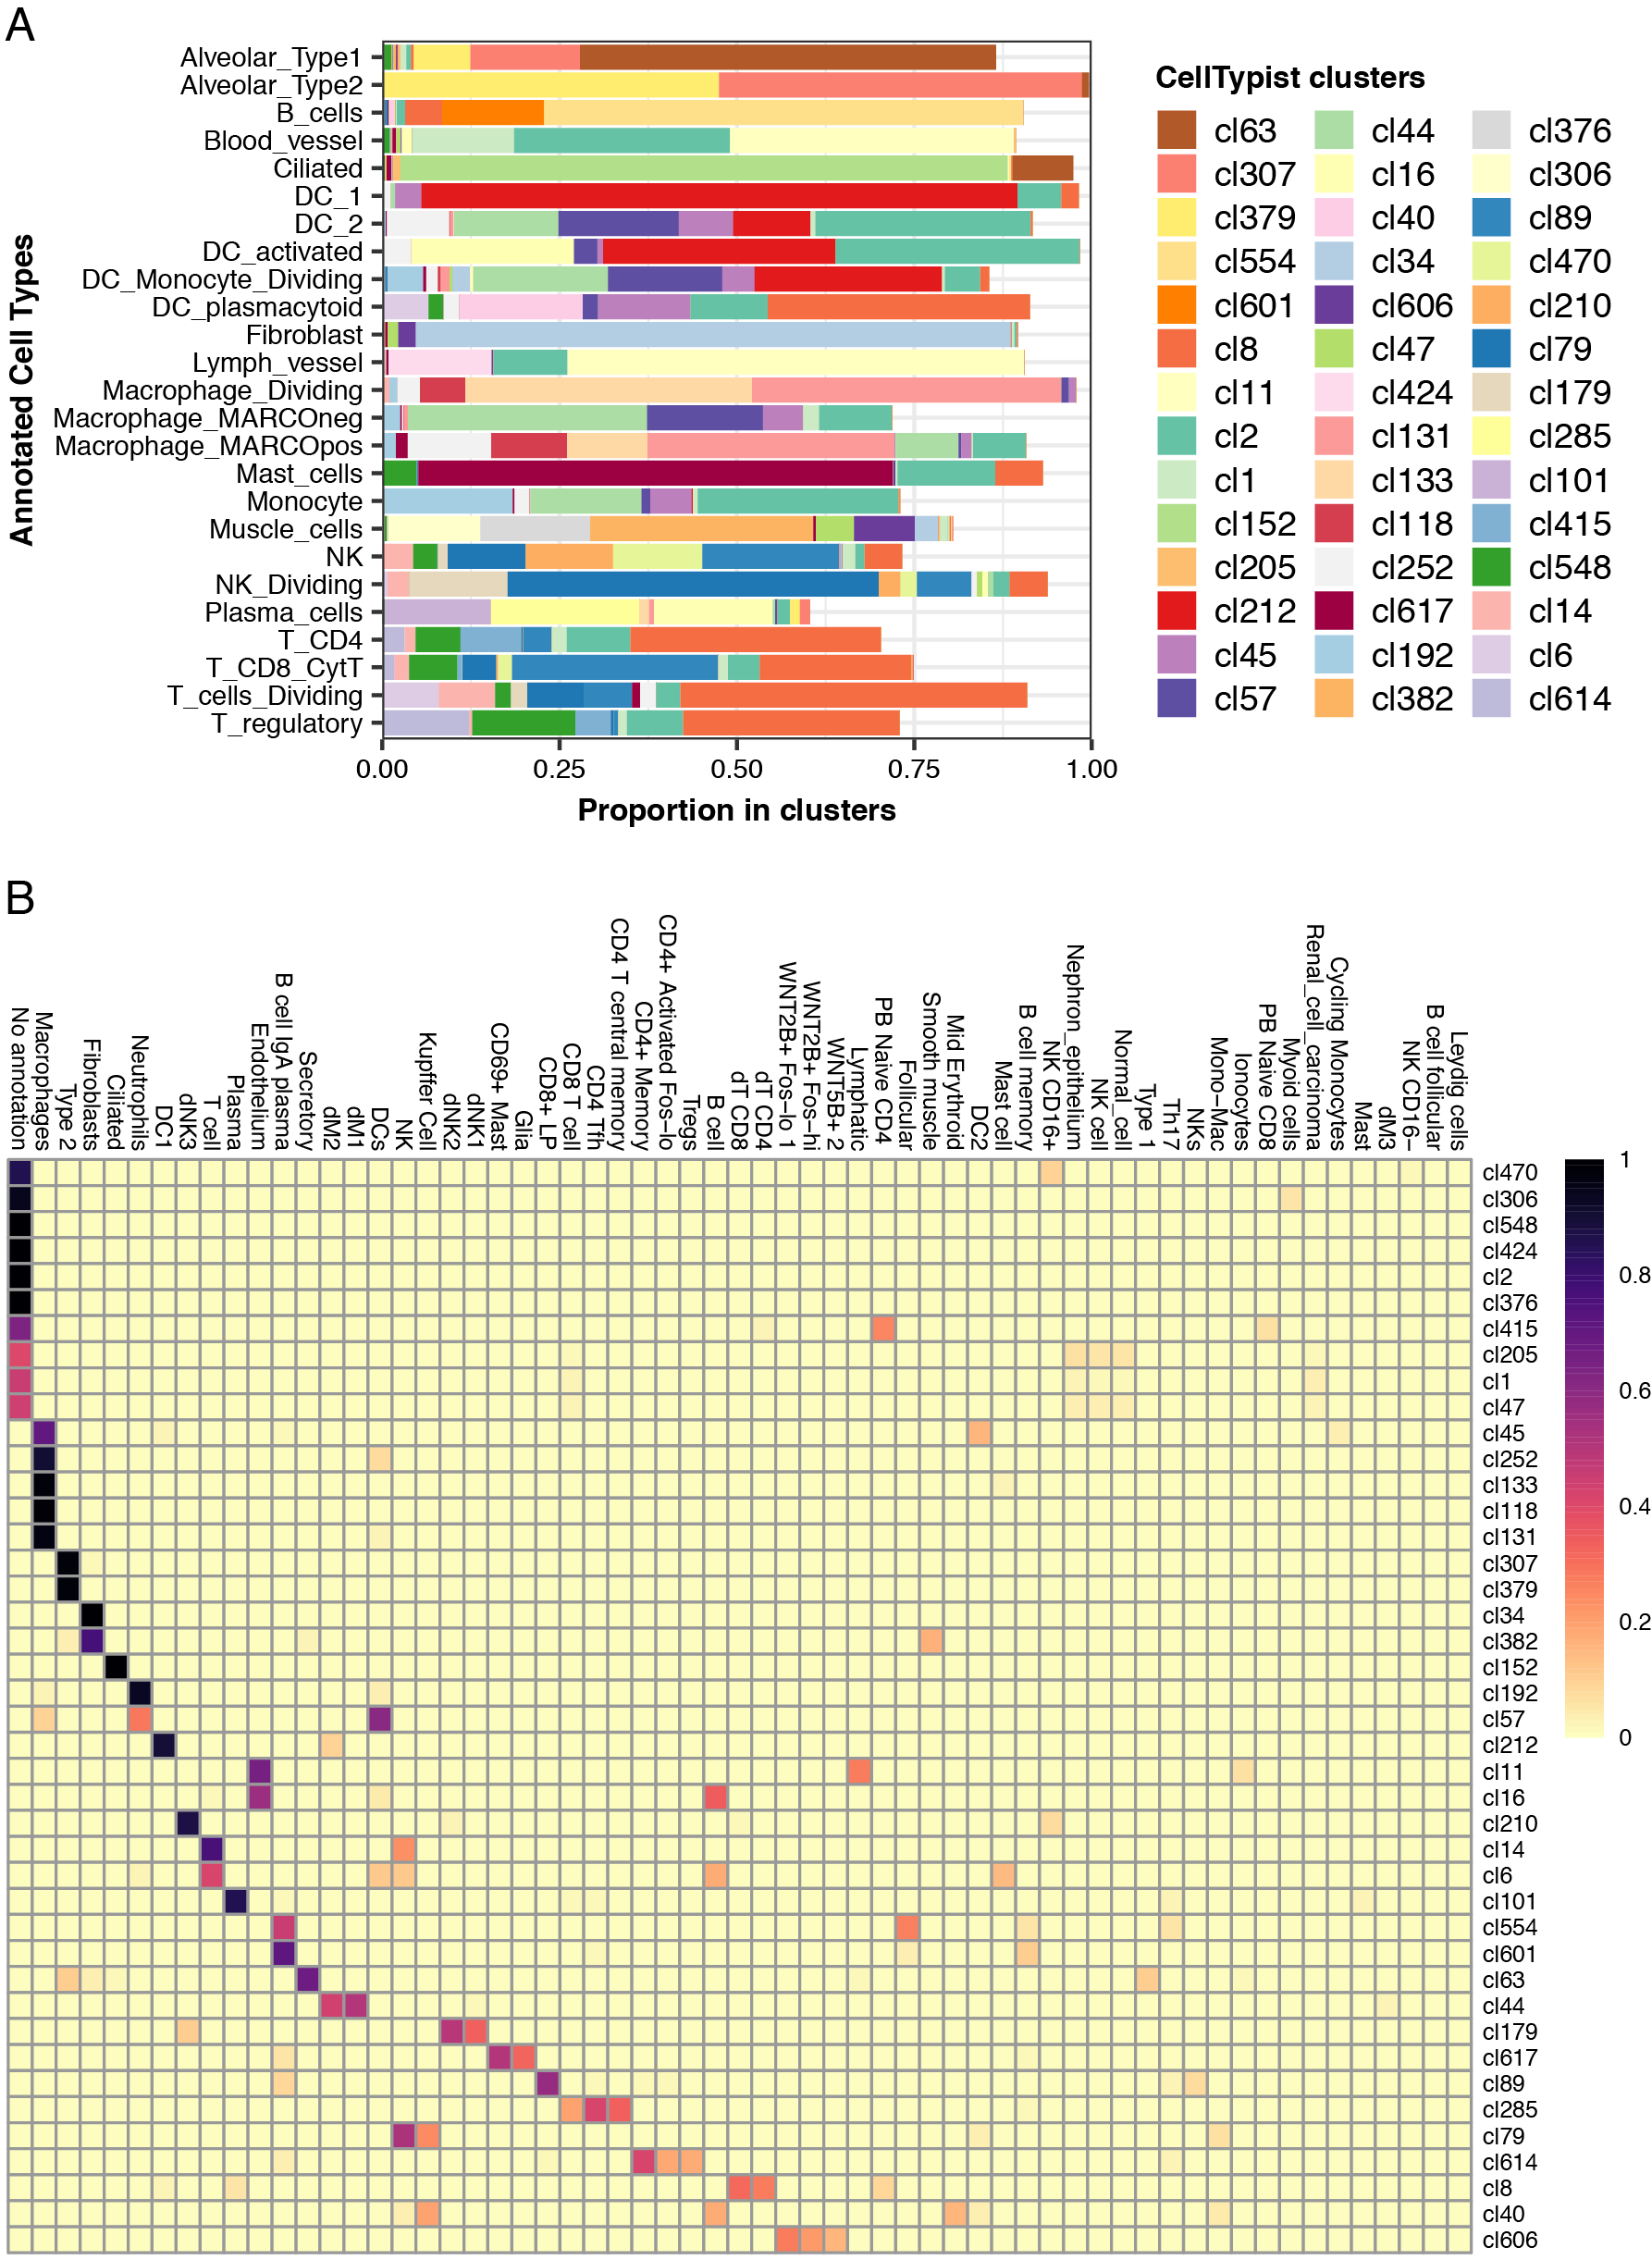
\includegraphics[scale=0.93]{Appendix3/Figs/appB_lung_labs_exp.png} % change word in curlies to change figure
\caption[Matching \textit{CellTypist} predictions in lung with annotations in the data collection]{\textbf{Matching \textit{CellTypist} predictions in lung with annotations in the data collection (Related to Figure~\ref{fig:chap4_preds})}\newline\textbf{(A)} \textit{CellTypist} clusters (thr1 = 0.99, thr2 = 0.8) matched to each original cell type annotation. Only the top 3 clusters per cell type were selected. \textbf{(B)} Proportion of cell type annotations (columns) represented in the \textit{CellTypist} clusters matched to lung.}
\label{fig:appB_lunglabs}
\end{figure}


\begin{figure}[ht!] 
\centering
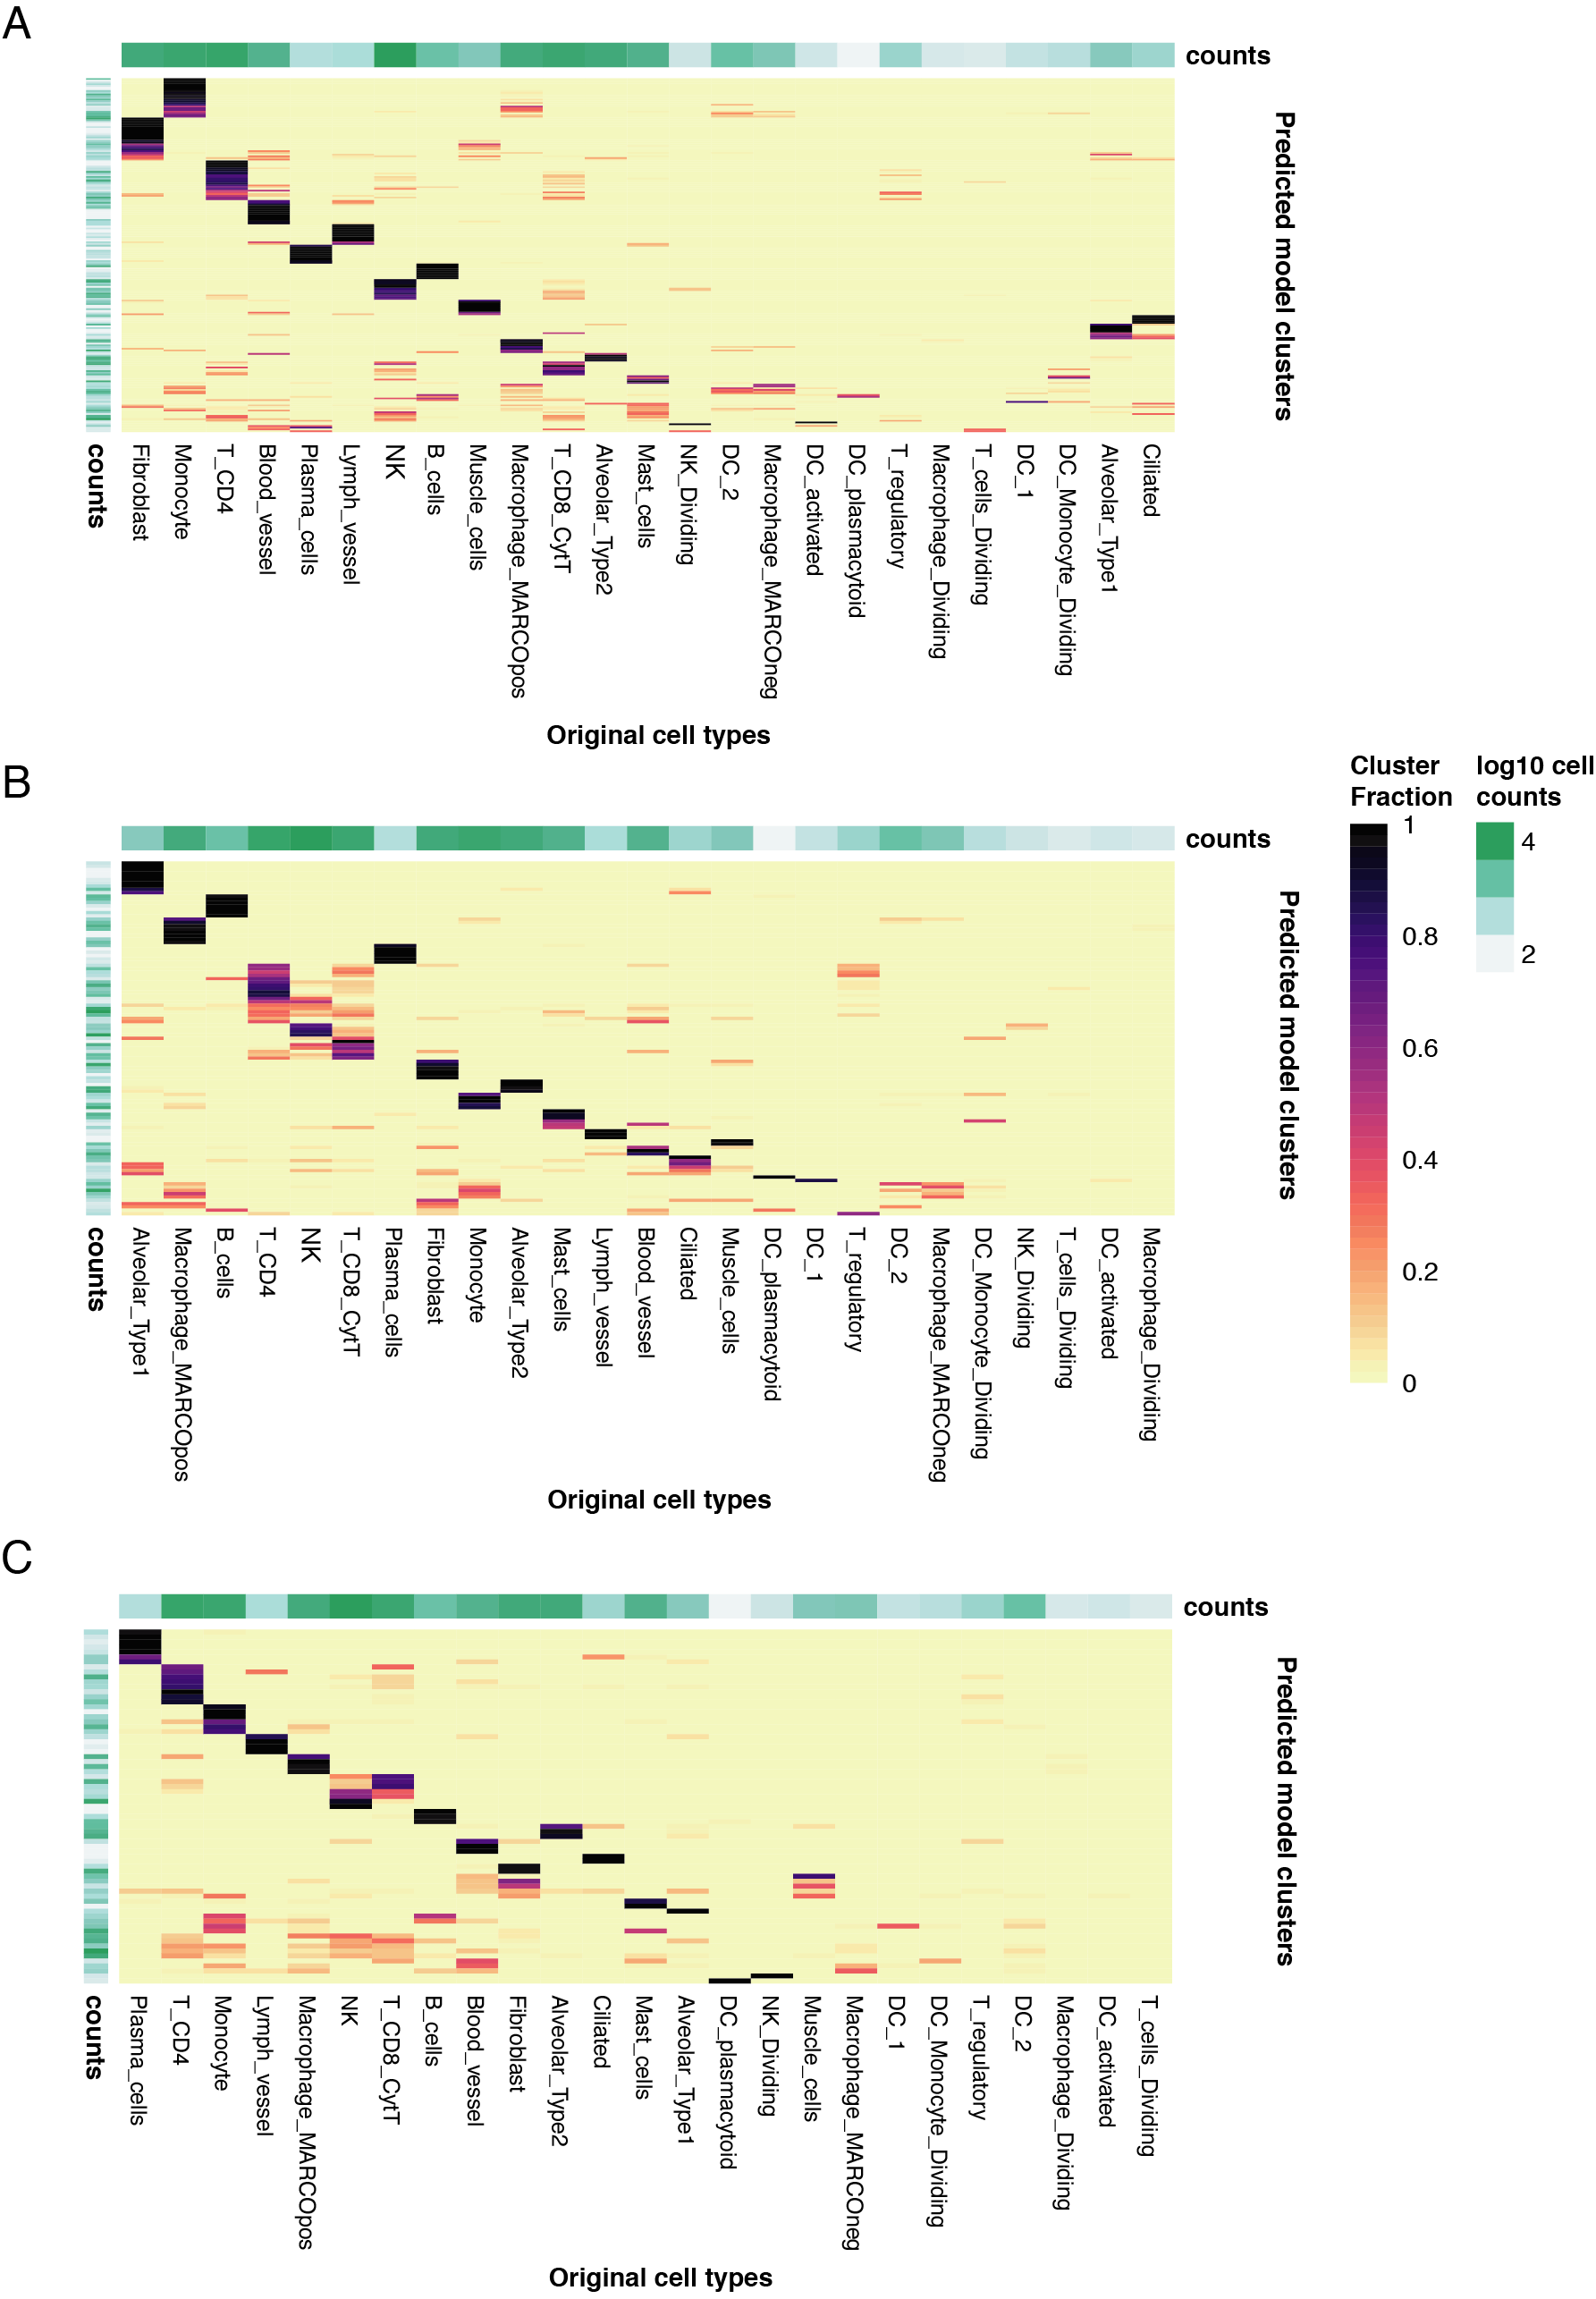
\includegraphics[scale=0.85]{Appendix3/Figs/appB_otherClustFrac_lung.png} % change word in curlies to change figure
\caption[Clusters matching lung annotated cell types in other \textit{CellTypist} models]{\textbf{Clusters matching lung annotated cell types in other \textit{CellTypist} models (Related to Figure~\ref{fig:chap4_preds}B)}\newline Proportion of clusters (rows) matching each annotated cell type (columns) in the models thr1 = 0.4, thr2 = 0.99 \textbf{(A)}, thr1 = 0.25, thr2 = 0.25 \textbf{(A)}, and thr1 = 0.1, thr2 = 0.1 \textbf{(C)}.}
\label{fig:appB_othercl}
\end{figure}


\begin{figure}[ht!] 
\centering
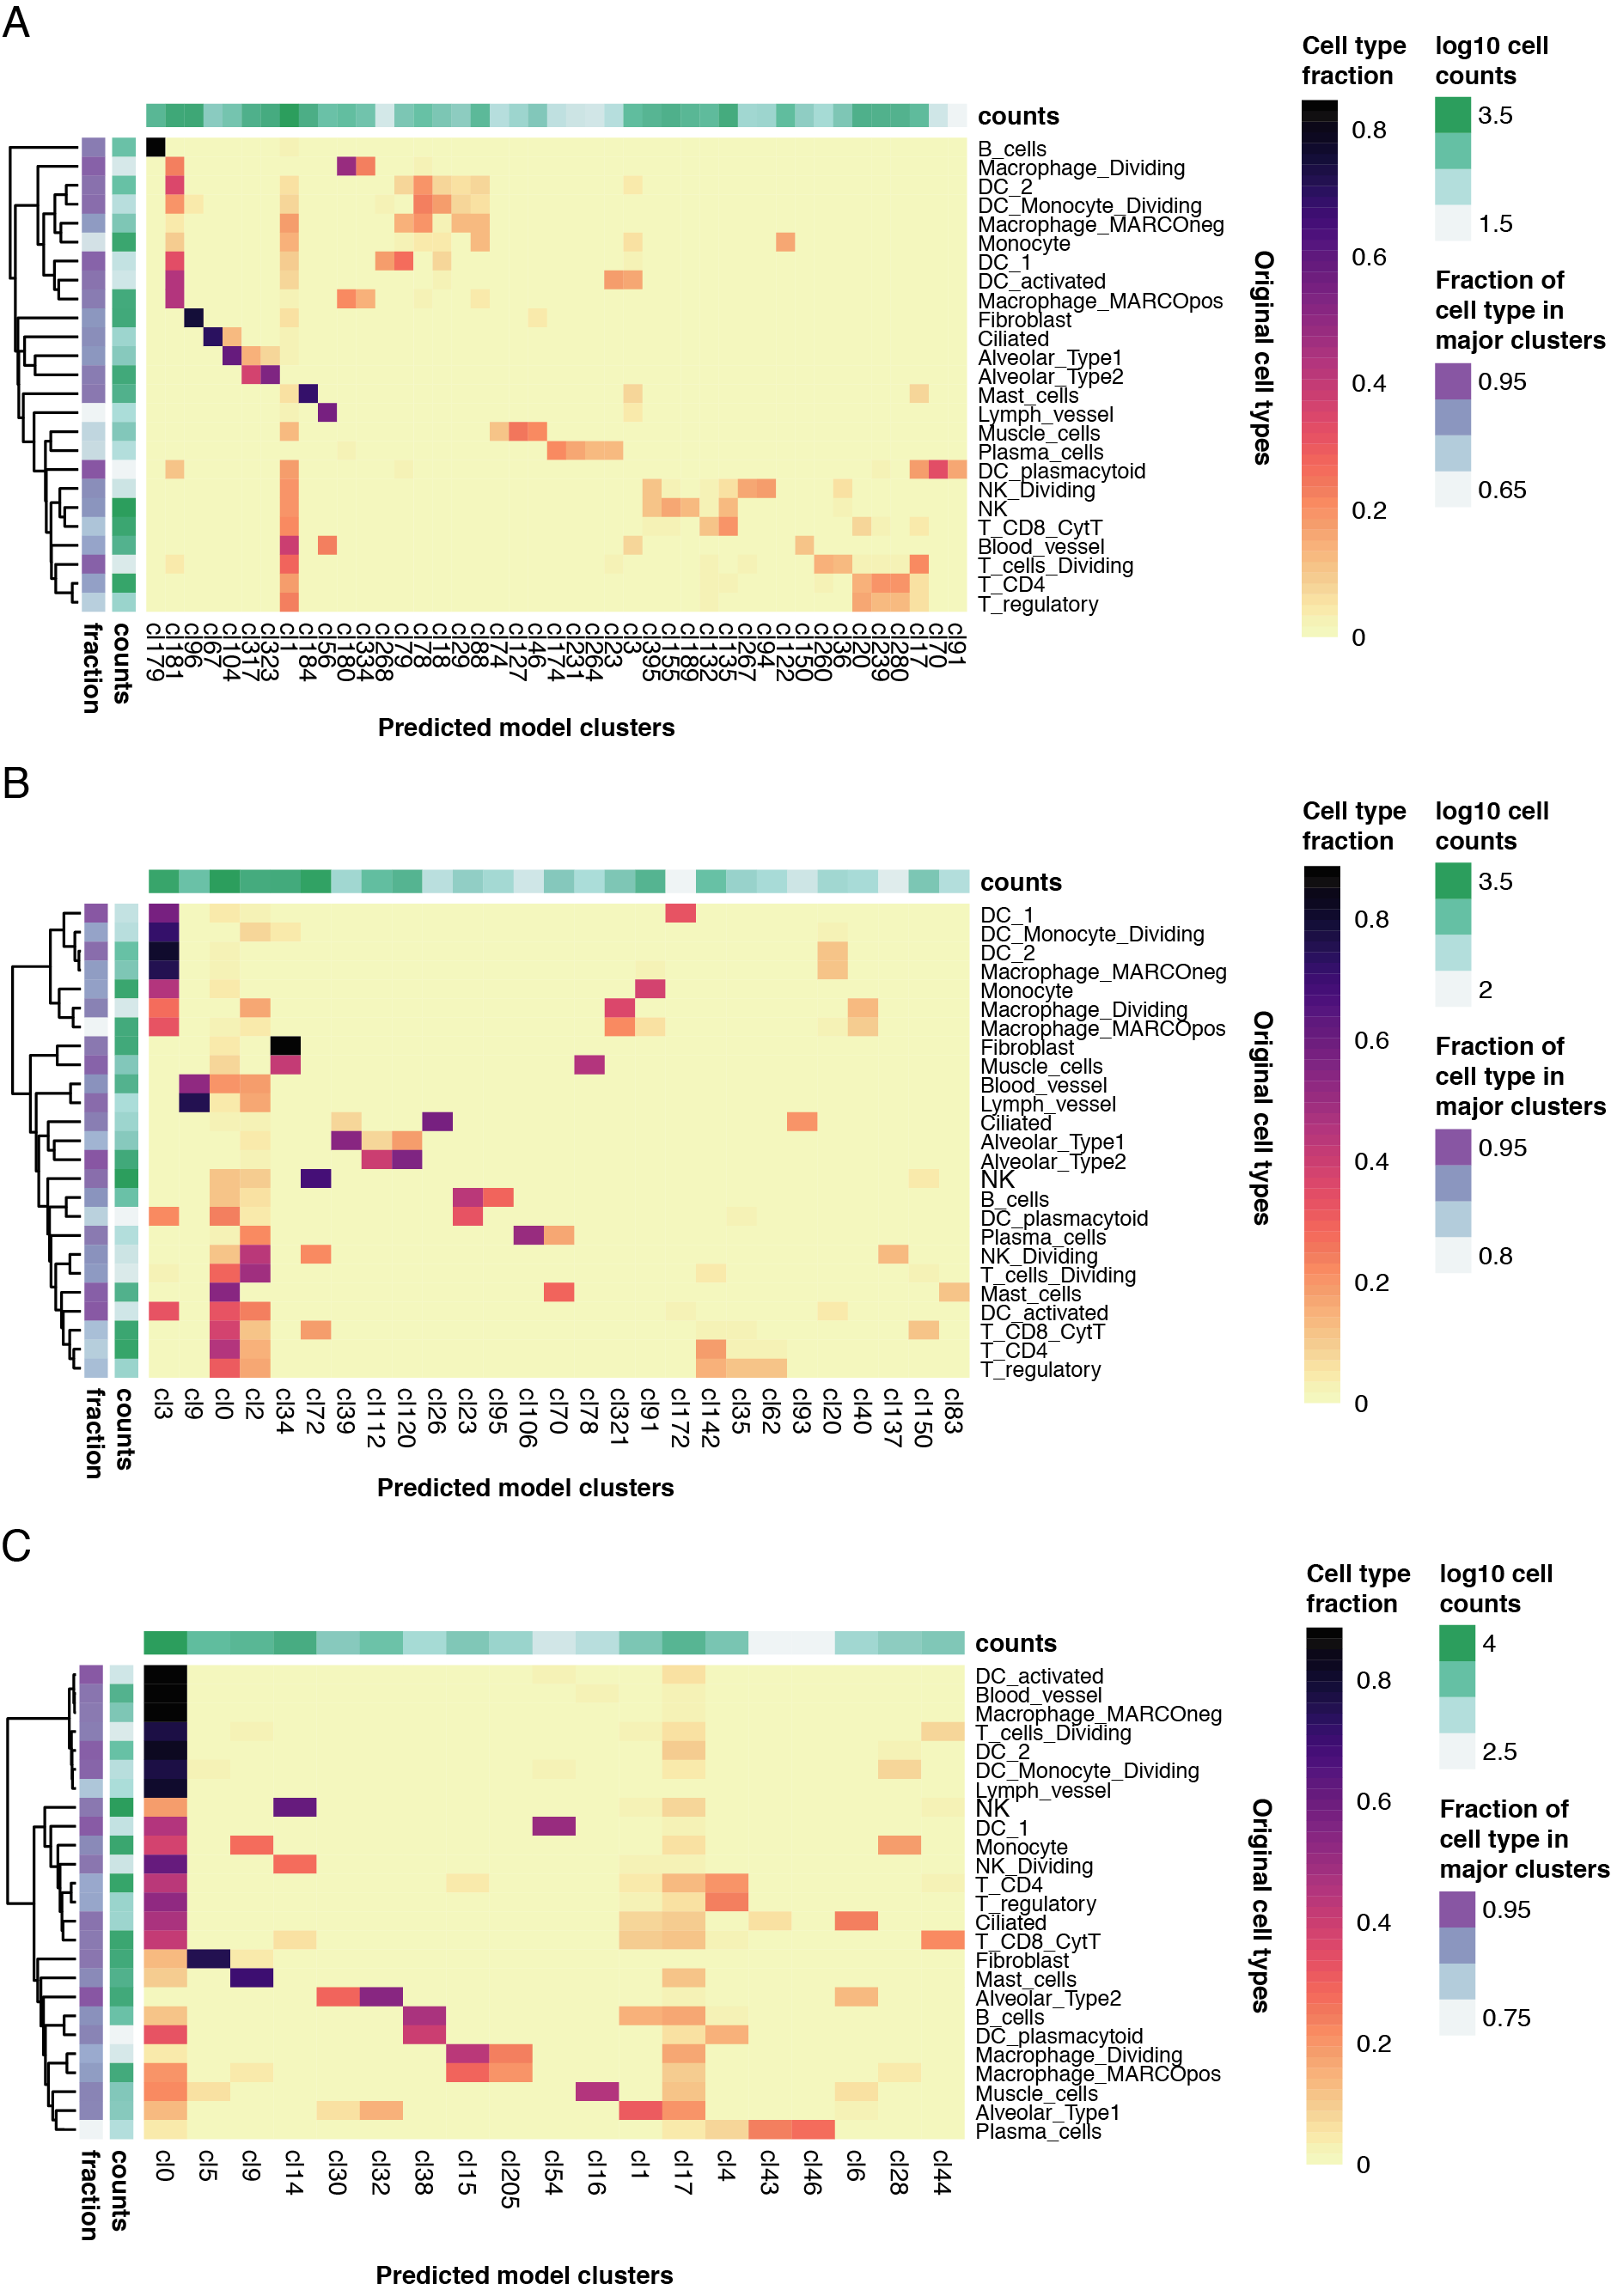
\includegraphics[scale=0.83]{Appendix3/Figs/appB_otherCtFrac_lung.png} % change word in curlies to change figure
\caption[Lung annotated cell types matching clusters in other \textit{CellTypist} models]{\textbf{Lung annotated cell types matching clusters in other \textit{CellTypist} models (Related to Figure~\ref{fig:chap4_preds}C)}\newline Proportion of annotated cell types (rows) included in each cluster (columns) in the models thr1 = 0.4, thr2 = 0.99 \textbf{(A)}, thr1 = 0.25, thr2 = 0.25 \textbf{(A)}, and thr1 = 0.1, thr2 = 0.1 \textbf{(C)}. Only clusters including at least 10\% of a given cell type were included.}
\label{fig:appB_otherct}
\end{figure}


\section{Supplementary Tables}
\label{sectionC1.2}

\begin{table}[pht!] % p for putting it in the next page available
\scriptsize
\caption[Cell types from~\citep{madissoon_lung_2019} with expression programmes enriched in \textit{CellTypist} clusters]{Cell types from~\citep{madissoon_lung_2019} with expression programmes enriched in \textit{CellTypist} clusters}
\centering
\label{table:tab_mad_match}
\begin{tabular}{lll}
  \toprule
Cluster & Tissue & Cell types \\ 
  \midrule
cl430 & Lung & Alveolar\_Type1 \\ 
  cl430 & Oesophagus & Epi\_upper,Epi\_stratified \\ 
  cl433 & Lung & Alveolar\_Type2 \\ 
  cl433 & Spleen & Plasmablast,DC\_1,Monocyte,NK\_dividing,Plasma\_IgG \\ 
  cl429 & Lung & Alveolar\_Type1 \\ 
  cl39 & Lung & T\_CD4,T\_cells\_Dividing,T\_regulatory \\ 
  cl39 & Spleen & T\_CD4\_fh,T\_CD4\_conv,T\_CD4\_reg,T\_CD8\_MAIT,T\_CD4\_naive \\ 
  cl39 & Oesophagus & T\_CD8,T\_CD4,NK\_T\_CD8\_Cytotoxic,Mast\_cell,Lymph\_vessel \\ 
  cl402 & Lung & Alveolar\_Type2,Alveolar\_Type1 \\ 
  cl402 & Oesophagus & Epi\_suprabasal \\ 
  cl318 & Lung & T\_cells\_Dividing,NK\_Dividing,DC\_Monocyte\_Dividing,Macrophage\_Dividing,Alveolar\_Type1 \\ 
  cl318 & Spleen & NK\_dividing,T\_cell\_dividing,B\_Hypermutation,Plasmablast,CD34\_progenitor \\ 
  cl318 & Oesophagus & Epi\_dividing \\ 
  cl416 & Lung & Alveolar\_Type1,Alveolar\_Type2,Ciliated,Lymph\_vessel \\ 
  cl416 & Oesophagus & Glands\_mucous,Epi\_basal,Glands\_duct,Epi\_suprabasal \\ 
  cl263 & Lung & Alveolar\_Type1,Alveolar\_Type2,Ciliated \\ 
  cl263 & Oesophagus & Epi\_stratified,Epi\_basal,Glands\_duct \\ 
  cl2 & Lung & DC\_2,DC\_activated,Lymph\_vessel,DC\_Monocyte\_Dividing,DC\_1 \\ 
  cl2 & Spleen & DC\_1,DC\_activated,DC\_2,DC\_plasmacytoid,T\_CD8\_gd \\ 
  cl2 & Oesophagus & Blood\_vessel,NK\_T\_CD8\_Cytotoxic,Mast\_cell,T\_CD8,Dendritic\_Cells \\ 
  cl1 & Lung & Blood\_vessel \\ 
  cl1 & Oesophagus & Blood\_vessel,Mast\_cell,Dendritic\_Cells,Stroma,NK\_T\_CD8\_Cytotoxic \\ 
  cl548 & Spleen & T\_CD8\_CTL,T\_CD8\_MAIT,T\_CD4\_conv \\ 
  cl548 & Oesophagus & T\_CD4,T\_CD8,NK\_T\_CD8\_Cytotoxic \\ 
  cl80 & Lung & Fibroblast,Muscle\_cells,Lymph\_vessel,Blood\_vessel \\ 
  cl80 & Spleen & T\_CD8\_MAIT,T\_CD8\_CTL \\ 
  cl80 & Oesophagus & Stroma,Epi\_basal,Lymph\_vessel,Glands\_duct,Epi\_suprabasal \\ 
  cl6 & Lung & T\_cells\_Dividing,DC\_Monocyte\_Dividing,DC\_1,DC\_activated,DC\_plasmacytoid \\ 
  cl6 & Spleen & T\_cell\_dividing,DC\_plasmacytoid,T\_CD8\_CTL,B\_Hypermutation,NK\_dividing \\ 
  cl6 & Oesophagus & Dendritic\_Cells,NK\_T\_CD8\_Cytotoxic,T\_CD8,T\_CD4,Mast\_cell \\ 
  cl614 & Lung & T\_CD4,T\_regulatory,T\_cells\_Dividing \\ 
  cl614 & Spleen & T\_CD4\_fh,T\_CD4\_reg,T\_CD4\_conv,T\_CD4\_naive \\ 
  cl614 & Oesophagus & T\_CD4,T\_CD8,NK\_T\_CD8\_Cytotoxic \\ 
  cl262 & Lung & Alveolar\_Type1,DC\_1,DC\_2,DC\_activated \\ 
  cl262 & Oesophagus & Epi\_stratified \\ 
  cl63 & Lung & Alveolar\_Type1,Alveolar\_Type2,Ciliated,Blood\_vessel,Lymph\_vessel \\ 
  cl63 & Spleen & DC\_activated,DC\_1,CD34\_progenitor,DC\_2,T\_CD8\_MAIT \\ 
  cl63 & Oesophagus & Glands\_duct,Epi\_basal,Glands\_mucous,Epi\_suprabasal,Lymph\_vessel \\ 
  cl513 & Lung & T\_CD4,T\_cells\_Dividing,T\_regulatory,Mast\_cells \\ 
  cl513 & Spleen & T\_CD4\_reg,T\_CD8\_MAIT,T\_CD4\_conv,T\_CD4\_fh,T\_cell\_dividing \\ 
  cl513 & Oesophagus & Mast\_cell,T\_CD4,NK\_T\_CD8\_Cytotoxic,T\_CD8 \\ 
  cl89 & Lung & NK\_Dividing,T\_CD8\_CytT,DC\_plasmacytoid,DC\_activated,NK \\ 
  cl89 & Spleen & T\_CD8\_activated,T\_CD8\_gd,T\_CD8\_MAIT,NK\_CD160pos,T\_CD8\_CTL \\ 
  cl89 & Oesophagus & NK\_T\_CD8\_Cytotoxic,T\_CD8,T\_CD4,B\_CD27pos,Mast\_cell \\ 
  cl377 & Lung & Alveolar\_Type2,Alveolar\_Type1 \\ 
  cl11 & Lung & Blood\_vessel,Lymph\_vessel,Muscle\_cells,Fibroblast,Alveolar\_Type2 \\ 
  cl11 & Spleen & B\_mantle,T\_cell\_dividing,NK\_dividing \\ 
  cl11 & Oesophagus & Blood\_vessel,Lymph\_vessel,Stroma,Epi\_basal \\ 
  cl424 & Lung & Lymph\_vessel,Blood\_vessel,Fibroblast \\ 
  cl424 & Oesophagus & Lymph\_vessel,Blood\_vessel \\ 
  cl329 & Lung & Ciliated,Mast\_cells,T\_CD4,Alveolar\_Type1,T\_CD8\_CytT \\ 
  cl329 & Spleen & T\_CD8\_gd,DC\_activated \\ 
  cl329 & Oesophagus & T\_CD4,T\_CD8,Glands\_duct,NK\_T\_CD8\_Cytotoxic,B\_CD27pos \\ 
  cl128 & Lung & Alveolar\_Type1,Alveolar\_Type2 \\ 
  cl128 & Oesophagus & Glands\_mucous,Epi\_stratified \\ 
  cl31 & Lung & Lymph\_vessel,Fibroblast,Alveolar\_Type1 \\ 
  cl31 & Spleen & DC\_activated,T\_CD4\_naive \\ 
  cl31 & Oesophagus & Lymph\_vessel,Epi\_basal \\ 
  cl8 & Lung & T\_cells\_Dividing,T\_CD4,T\_CD8\_CytT,T\_regulatory,DC\_plasmacytoid \\ 
  cl8 & Spleen & T\_CD4\_reg,T\_CD4\_conv,T\_CD8\_activated,T\_cell\_dividing,T\_CD8\_CTL \\ 
  cl8 & Oesophagus & T\_CD4,T\_CD8,NK\_T\_CD8\_Cytotoxic,Mast\_cell,B\_CD27neg \\ 
   \bottomrule
\end{tabular}
\end{table}  
  
\begin{table}[pht!] % p for putting it in the next page available
\scriptsize
\caption[Cell types from~\citep{madissoon_lung_2019} with expression programmes enriched in \textit{CellTypist} clusters (continued 1)]{Cell types from~\citep{madissoon_lung_2019} with expression programmes enriched in \textit{CellTypist} clusters (continued 1)}
\centering
\label{table:tab_mad_match1}
\begin{tabular}{lll}
  \toprule
Cluster & Tissue & Cell types \\ 
  \midrule
cl554 & Lung & B\_cells,DC\_plasmacytoid,DC\_activated,T\_cells\_Dividing \\ 
  cl554 & Spleen & B\_follicular,B\_mantle,B\_Hypermutation \\ 
  cl554 & Oesophagus & B\_CD27pos,B\_CD27neg,T\_CD4,Dendritic\_Cells,NK\_T\_CD8\_Cytotoxic \\ 
  cl425 & Lung & Lymph\_vessel,Blood\_vessel,Muscle\_cells,Fibroblast \\ 
  cl425 & Spleen & DC\_1 \\ 
  cl425 & Oesophagus & Lymph\_vessel,Blood\_vessel,Stroma,Epi\_basal,Glands\_duct \\ 
  cl210 & Lung & NK\_Dividing,NK,T\_cells\_Dividing,DC\_plasmacytoid,DC\_1 \\ 
  cl210 & Spleen & NK\_CD160pos,NK\_FCGR3Apos,T\_CD8\_gd,NK\_dividing,T\_CD8\_MAIT \\ 
  cl210 & Oesophagus & NK\_T\_CD8\_Cytotoxic,T\_CD8,T\_CD4,Dendritic\_Cells,B\_CD27pos \\ 
  cl87 & Lung & T\_CD4 \\ 
  cl87 & Spleen & T\_CD8\_MAIT,Monocyte \\ 
  cl87 & Oesophagus & T\_CD4,T\_CD8,NK\_T\_CD8\_Cytotoxic,Mast\_cell \\ 
  cl47 & Lung & Fibroblast,Muscle\_cells,NK\_Dividing,Blood\_vessel,Lymph\_vessel \\ 
  cl47 & Oesophagus & Stroma,Blood\_vessel,Epi\_basal,Lymph\_vessel \\ 
  cl222 & Lung & Lymph\_vessel,Blood\_vessel,Fibroblast \\ 
  cl222 & Oesophagus & Lymph\_vessel,Blood\_vessel,Stroma \\ 
  cl88 & Lung & Blood\_vessel,Lymph\_vessel,Alveolar\_Type1,DC\_activated,Muscle\_cells \\ 
  cl88 & Spleen & T\_CD8\_MAIT,T\_CD4\_conv,T\_CD4\_naive,DC\_activated \\ 
  cl88 & Oesophagus & Blood\_vessel,Lymph\_vessel,Epi\_basal,Glands\_duct,Stroma \\ 
  cl73 & Lung & T\_cells\_Dividing,T\_CD4,T\_regulatory,DC\_activated \\ 
  cl73 & Spleen & T\_CD4\_reg,T\_CD8\_MAIT,ILC,T\_CD4\_fh,T\_CD4\_conv \\ 
  cl73 & Oesophagus & T\_CD4,T\_CD8,NK\_T\_CD8\_Cytotoxic,Mast\_cell,B\_CD27pos \\ 
  cl606 & Lung & Fibroblast,Muscle\_cells,DC\_activated,Macrophage\_MARCOpos,Macrophage\_MARCOneg \\ 
  cl606 & Spleen & Monocyte,DC\_1,DC\_2,Macrophage \\ 
  cl606 & Oesophagus & Stroma,Mast\_cell,Epi\_suprabasal,Mono\_macro,Lymph\_vessel \\ 
  cl449 & Spleen & T\_cell\_dividing,T\_CD4\_conv,T\_CD4\_fh,B\_Hypermutation,CD34\_progenitor \\ 
  cl449 & Oesophagus & Lymph\_vessel,Blood\_vessel,Glands\_duct \\ 
  cl58 & Lung & T\_regulatory,T\_cells\_Dividing,T\_CD4,T\_CD8\_CytT,Mast\_cells \\ 
  cl58 & Spleen & NK\_CD160pos,T\_CD4\_reg,T\_CD8\_gd,T\_CD8\_MAIT,T\_CD8\_CTL \\ 
  cl58 & Oesophagus & T\_CD8,T\_CD4,NK\_T\_CD8\_Cytotoxic,Mast\_cell,Dendritic\_Cells \\ 
  cl74 & Lung & Alveolar\_Type1 \\ 
  cl74 & Oesophagus & Epi\_basal,Glands\_duct \\ 
  cl147 & Spleen & CD34\_progenitor \\ 
  cl71 & Lung & T\_CD8\_CytT \\ 
  cl71 & Spleen & T\_CD8\_MAIT,T\_CD8\_activated,T\_CD8\_CTL,T\_CD8\_gd \\ 
  cl71 & Oesophagus & T\_CD4,T\_CD8 \\ 
  cl616 & Lung & T\_CD8\_CytT,NK\_Dividing,NK,T\_regulatory,T\_cells\_Dividing \\ 
  cl616 & Spleen & T\_CD8\_activated,T\_CD8\_MAIT,T\_CD8\_gd,NK\_CD160pos,T\_CD4\_fh \\ 
  cl616 & Oesophagus & T\_CD8,NK\_T\_CD8\_Cytotoxic,T\_CD4 \\ 
  cl179 & Lung & NK\_Dividing,NK,T\_cells\_Dividing \\ 
  cl179 & Spleen & NK\_dividing,NK\_CD160pos,T\_CD8\_gd,NK\_FCGR3Apos,ILC \\ 
  cl179 & Oesophagus & NK\_T\_CD8\_Cytotoxic,T\_CD8,Epi\_dividing,T\_CD4,Mast\_cell \\ 
  cl34 & Lung & Fibroblast,Muscle\_cells,Monocyte \\ 
  cl34 & Spleen & Monocyte,T\_CD8\_CTL \\ 
  cl34 & Oesophagus & Stroma,Lymph\_vessel,Dendritic\_Cells,Epi\_basal,Mono\_macro \\ 
  cl271 & Lung & Fibroblast,Muscle\_cells,Lymph\_vessel,Blood\_vessel \\ 
  cl271 & Oesophagus & Stroma,Lymph\_vessel,Epi\_basal,Blood\_vessel,Epi\_suprabasal \\ 
  cl172 & Lung & Lymph\_vessel,Blood\_vessel,Fibroblast \\ 
  cl172 & Oesophagus & Lymph\_vessel,Blood\_vessel,Stroma,Epi\_basal,Epi\_suprabasal \\ 
  cl435 & Lung & Macrophage\_MARCOneg,Macrophage\_MARCOpos \\ 
  cl435 & Spleen & Macrophage,DC\_2,Monocyte \\ 
  cl79 & Lung & NK\_Dividing,NK,T\_CD8\_CytT,T\_cells\_Dividing,T\_regulatory \\ 
  cl79 & Spleen & T\_CD8\_activated,NK\_dividing,T\_CD8\_gd,T\_CD8\_CTL,NK\_CD160pos \\ 
  cl79 & Oesophagus & NK\_T\_CD8\_Cytotoxic,T\_CD8,T\_CD4,Epi\_dividing,Mono\_macro \\ 
  cl36 & Lung & Blood\_vessel,DC\_activated,DC\_Monocyte\_Dividing,DC\_plasmacytoid,Macrophage\_MARCOpos \\ 
  cl36 & Spleen & DC\_2,DC\_activated,DC\_1,B\_follicular,Macrophage \\ 
  cl36 & Oesophagus & Blood\_vessel,Dendritic\_Cells,Mono\_macro,B\_CD27pos,B\_CD27neg \\ 
  cl505 & Spleen & Monocyte \\ 
  cl404 & Lung & Muscle\_cells,Fibroblast \\ 
  cl404 & Oesophagus & Epi\_suprabasal \\ 
   \bottomrule
\end{tabular}
\end{table}  
  
\begin{table}[pht!] % p for putting it in the next page available
\scriptsize
\caption[Cell types from~\citep{madissoon_lung_2019} with expression programmes enriched in \textit{CellTypist} clusters (continued 2)]{Cell types from~\citep{madissoon_lung_2019} with expression programmes enriched in \textit{CellTypist} clusters (continued 2)}
\centering
\label{table:tab_mad_match2}
\begin{tabular}{lll}
  \toprule
Cluster & Tissue & Cell types \\ 
  \midrule
  cl464 & Lung & Macrophage\_MARCOneg \\ 
  cl464 & Spleen & CD34\_progenitor,DC\_2 \\ 
  cl464 & Oesophagus & Dendritic\_Cells \\ 
  cl596 & Lung & T\_CD4,T\_cells\_Dividing,T\_regulatory,Mast\_cells,B\_cells \\ 
  cl596 & Spleen & T\_CD8\_MAIT,T\_CD4\_conv,T\_CD4\_fh,T\_CD4\_reg,T\_CD4\_naive \\ 
  cl596 & Oesophagus & T\_CD8,NK\_T\_CD8\_Cytotoxic,T\_CD4,Dendritic\_Cells,B\_CD27pos \\ 
  cl45 & Lung & DC\_2,Macrophage\_MARCOneg,DC\_1,DC\_Monocyte\_Dividing,DC\_plasmacytoid \\ 
  cl45 & Spleen & DC\_2,DC\_1,DC\_activated,DC\_plasmacytoid,Monocyte \\ 
  cl45 & Oesophagus & Dendritic\_Cells,Mono\_macro,B\_CD27pos,B\_CD27neg,Blood\_vessel \\ 
  cl51 & Lung & DC\_2,Macrophage\_MARCOneg,DC\_1,DC\_activated,DC\_Monocyte\_Dividing \\ 
  cl51 & Spleen & DC\_2,DC\_1,DC\_activated,Monocyte,Macrophage \\ 
  cl51 & Oesophagus & Dendritic\_Cells,Mono\_macro,T\_CD4,B\_CD27pos,B\_CD27neg \\ 
  cl441 & Spleen & T\_CD4\_naive \\ 
  cl432 & Lung & Alveolar\_Type1,Ciliated,Alveolar\_Type2 \\ 
  cl432 & Spleen & B\_mantle \\ 
  cl432 & Oesophagus & Glands\_duct,Glands\_mucous,Epi\_basal \\ 
  cl617 & Lung & DC\_2,Mast\_cells,Muscle\_cells \\ 
  cl617 & Spleen & Monocyte,T\_CD8\_MAIT \\ 
  cl617 & Oesophagus & Mast\_cell,Dendritic\_Cells,Epi\_basal,B\_CD27pos,Mono\_macro \\ 
  cl260 & Lung & DC\_plasmacytoid,Alveolar\_Type1,Ciliated,Monocyte,DC\_activated \\ 
  cl260 & Spleen & CD34\_progenitor \\ 
  cl260 & Oesophagus & Blood\_vessel,Epi\_suprabasal \\ 
  cl452 & Lung & Monocyte \\ 
  cl452 & Spleen & Monocyte \\ 
  cl27 & Lung & Blood\_vessel,Lymph\_vessel,Muscle\_cells \\ 
  cl27 & Oesophagus & Blood\_vessel,Lymph\_vessel,Stroma \\ 
  cl64 & Lung & Blood\_vessel,Lymph\_vessel,Fibroblast,Muscle\_cells \\ 
  cl64 & Spleen & T\_CD4\_conv \\ 
  cl64 & Oesophagus & Blood\_vessel,Lymph\_vessel,Stroma,Epi\_basal \\ 
  cl205 & Lung & T\_CD8\_CytT \\ 
  cl205 & Spleen & T\_CD8\_gd,T\_CD8\_CTL \\ 
  cl252 & Lung & Macrophage\_MARCOpos,Macrophage\_Dividing,DC\_activated,DC\_Monocyte\_Dividing,DC\_2 \\ 
  cl252 & Spleen & DC\_2,DC\_1,NK\_dividing,DC\_activated,CD34\_progenitor \\ 
  cl252 & Oesophagus & NK\_T\_CD8\_Cytotoxic,T\_CD4,Mast\_cell,Mono\_macro,T\_CD8 \\ 
  cl76 & Spleen & Monocyte \\ 
  cl508 & Lung & T\_CD8\_CytT,T\_CD4,T\_regulatory,NK,NK\_Dividing \\ 
  cl508 & Spleen & T\_CD8\_CTL,T\_CD8\_MAIT,T\_CD8\_activated,T\_CD8\_gd,T\_CD4\_fh \\ 
  cl508 & Oesophagus & T\_CD8,T\_CD4,NK\_T\_CD8\_Cytotoxic \\ 
  cl621 & Lung & T\_cells\_Dividing,T\_CD4,T\_regulatory,DC\_activated \\ 
  cl621 & Spleen & T\_CD8\_MAIT,T\_CD4\_reg,T\_cell\_dividing,Monocyte,T\_CD4\_conv \\ 
  cl621 & Oesophagus & T\_CD4,T\_CD8,Dendritic\_Cells,NK\_T\_CD8\_Cytotoxic,Mast\_cell \\ 
  cl512 & Lung & Monocyte,Macrophage\_MARCOneg,Macrophage\_MARCOpos,DC\_1,DC\_2 \\ 
  cl512 & Spleen & Monocyte,DC\_2,Macrophage,DC\_activated,DC\_1 \\ 
  cl512 & Oesophagus & Mono\_macro,Dendritic\_Cells,B\_CD27pos,B\_CD27neg,T\_CD4 \\ 
  cl70 & Lung & DC\_Monocyte\_Dividing,DC\_1,Macrophage\_Dividing,DC\_activated,Macrophage\_MARCOpos \\ 
  cl70 & Spleen & DC\_1,DC\_2,DC\_activated,B\_follicular,B\_mantle \\ 
  cl70 & Oesophagus & Dendritic\_Cells,Blood\_vessel,Mono\_macro,B\_CD27pos,B\_CD27neg \\ 
  cl568 & Lung & Ciliated \\ 
  cl340 & Lung & Fibroblast,Lymph\_vessel \\ 
  cl340 & Spleen & DC\_plasmacytoid \\ 
  cl340 & Oesophagus & Glands\_mucous,Stroma,Epi\_basal,Lymph\_vessel \\ 
  cl57 & Lung & Macrophage\_MARCOneg,DC\_2,DC\_Monocyte\_Dividing,DC\_activated,DC\_1 \\ 
  cl57 & Spleen & DC\_2,Monocyte,DC\_1,DC\_activated,DC\_plasmacytoid \\ 
  cl57 & Oesophagus & Dendritic\_Cells,Mono\_macro,Lymph\_vessel,Mast\_cell,Blood\_vessel \\ 
  cl491 & Lung & Macrophage\_Dividing,DC\_Monocyte\_Dividing,Macrophage\_MARCOpos,DC\_activated,DC\_2 \\ 
  cl491 & Spleen & DC\_2,DC\_1,Monocyte,Macrophage,DC\_activated \\ 
  cl491 & Oesophagus & Dendritic\_Cells,Mono\_macro,B\_CD27neg,T\_CD4,B\_CD27pos \\ 
   \bottomrule
\end{tabular}
\end{table}  
  
\begin{table}[pht!] % p for putting it in the next page available
\scriptsize
\caption[Cell types from~\citep{madissoon_lung_2019} with expression programmes enriched in \textit{CellTypist} clusters (continued 3)]{Cell types from~\citep{madissoon_lung_2019} with expression programmes enriched in \textit{CellTypist} clusters (continued 3)}
\centering
\label{table:tab_mad_match3}
\begin{tabular}{lll}
  \toprule
Cluster & Tissue & Cell types \\ 
  \midrule
  cl100 & Lung & Blood\_vessel,DC\_plasmacytoid,Lymph\_vessel,Muscle\_cells,DC\_2 \\ 
  cl100 & Spleen & DC\_plasmacytoid,DC\_2,B\_follicular,B\_mantle,DC\_1 \\ 
  cl100 & Oesophagus & Blood\_vessel,Dendritic\_Cells,Lymph\_vessel,Stroma,Mono\_macro \\ 
  cl46 & Lung & DC\_activated,DC\_1,DC\_Monocyte\_Dividing,Macrophage\_MARCOneg,Macrophage\_MARCOpos \\ 
  cl46 & Spleen & DC\_activated,DC\_2,DC\_1,B\_follicular,B\_Hypermutation \\ 
  cl46 & Oesophagus & Dendritic\_Cells,Blood\_vessel,Mono\_macro,B\_CD27neg,B\_CD27pos \\ 
  cl44 & Lung & DC\_2,Macrophage\_MARCOneg,DC\_Monocyte\_Dividing,Macrophage\_MARCOpos,Monocyte \\ 
  cl44 & Spleen & Monocyte,DC\_2,DC\_activated,Macrophage,T\_CD4\_conv \\ 
  cl44 & Oesophagus & Mono\_macro,Dendritic\_Cells,T\_CD8,B\_CD27neg,NK\_T\_CD8\_Cytotoxic \\ 
  cl503 & Lung & DC\_2,Macrophage\_MARCOneg,Monocyte,DC\_activated \\ 
  cl503 & Spleen & Monocyte,Macrophage \\ 
  cl503 & Oesophagus & Epi\_basal,Blood\_vessel,Mono\_macro,Glands\_duct \\ 
  cl25 & Lung & \specialcell[t]{Macrophage\_MARCOneg,Macrophage\_MARCOpos,\\DC\_2,Macrophage\_Dividing,DC\_Monocyte\_Dividing} \\ 
  cl25 & Spleen & DC\_2,Monocyte,Macrophage,DC\_1,DC\_plasmacytoid \\ 
  cl25 & Oesophagus & Mono\_macro,Dendritic\_Cells,Mast\_cell,Glands\_duct,Lymph\_vessel \\ 
  cl93 & Lung & Monocyte,Macrophage\_MARCOpos \\ 
  cl93 & Spleen & Monocyte \\ 
  cl485 & Lung & Plasma\_cells,DC\_1 \\ 
  cl485 & Spleen & Plasma\_IgG,Plasma\_IgM,Monocyte \\ 
  cl577 & Lung & Alveolar\_Type2,Alveolar\_Type1 \\ 
  cl577 & Spleen & B\_follicular \\ 
  cl577 & Oesophagus & Epi\_upper \\ 
  cl316 & Lung & Alveolar\_Type1 \\ 
  cl316 & Oesophagus & Glands\_mucous,Glands\_duct,Epi\_upper,Epi\_basal \\ 
  cl220 & Lung & Ciliated \\ 
  cl611 & Lung & T\_CD4,T\_regulatory,DC\_activated,T\_cells\_Dividing,DC\_2 \\ 
  cl611 & Spleen & T\_CD8\_MAIT,T\_CD4\_conv,ILC,T\_CD4\_fh,T\_cell\_dividing \\ 
  cl611 & Oesophagus & NK\_T\_CD8\_Cytotoxic,T\_CD4,T\_CD8 \\ 
  cl242 & Lung & Fibroblast \\ 
  cl242 & Oesophagus & Stroma,Epi\_basal \\ 
  cl458 & Lung & NK\_Dividing,NK,T\_CD8\_CytT \\ 
  cl458 & Spleen & T\_CD8\_CTL,NK\_FCGR3Apos,NK\_CD160pos,NK\_dividing,T\_CD8\_MAIT \\ 
  cl458 & Oesophagus & T\_CD8,NK\_T\_CD8\_Cytotoxic,T\_CD4 \\ 
  cl417 & Lung & Lymph\_vessel,Alveolar\_Type1 \\ 
  cl417 & Spleen & DC\_1 \\ 
  cl417 & Oesophagus & Glands\_duct,Glands\_mucous \\ 
  cl401 & Lung & DC\_2,DC\_activated \\ 
  cl401 & Oesophagus & Glands\_mucous,Glands\_duct \\ 
  cl581 & Lung & Alveolar\_Type2,Alveolar\_Type1,Ciliated \\ 
  cl581 & Oesophagus & Epi\_basal \\ 
  cl592 & Lung & DC\_plasmacytoid \\ 
  cl592 & Spleen & B\_follicular,B\_mantle \\ 
  cl592 & Oesophagus & B\_CD27pos,B\_CD27neg \\ 
  cl376 & Lung & Muscle\_cells,Fibroblast,Ciliated \\ 
  cl376 & Oesophagus & Stroma,Lymph\_vessel,Mast\_cell \\ 
  cl519 & Lung & T\_regulatory,T\_CD4,T\_cells\_Dividing \\ 
  cl519 & Spleen & T\_CD8\_MAIT,T\_CD4\_fh,T\_CD4\_conv,T\_CD4\_reg \\ 
  cl519 & Oesophagus & T\_CD4,NK\_T\_CD8\_Cytotoxic,T\_CD8,Mast\_cell \\ 
  cl35 & Lung & \specialcell[t]{Macrophage\_MARCOpos,DC\_Monocyte\_Dividing,DC\_1,\\Macrophage\_Dividing,Macrophage\_MARCOneg} \\ 
  cl35 & Spleen & DC\_1,DC\_2,DC\_activated,Monocyte,B\_mantle \\ 
  cl35 & Oesophagus & Mono\_macro,Dendritic\_Cells,B\_CD27neg,Glands\_duct,B\_CD27pos \\ 
  cl446 & Lung & T\_CD4,T\_CD8\_CytT,T\_regulatory \\ 
  cl446 & Spleen & T\_CD4\_fh,T\_CD4\_reg,T\_CD8\_MAIT,T\_CD4\_naive \\ 
  cl446 & Oesophagus & T\_CD4,T\_CD8,NK\_T\_CD8\_Cytotoxic \\ 
  cl219 & Lung & Blood\_vessel,Muscle\_cells,Lymph\_vessel,Alveolar\_Type1,Fibroblast \\ 
  cl219 & Oesophagus & Blood\_vessel,Lymph\_vessel,Stroma,Epi\_basal \\ 
     \bottomrule
\end{tabular}
\end{table}  
  
\begin{table}[pht!] % p for putting it in the next page available
\scriptsize
\caption[Cell types from~\citep{madissoon_lung_2019} with expression programmes enriched in \textit{CellTypist} clusters (continued 4)]{Cell types from~\citep{madissoon_lung_2019} with expression programmes enriched in \textit{CellTypist} clusters (continued 4)}
\centering
\label{table:tab_mad_match4}
\begin{tabular}{lll}
  \toprule
Cluster & Tissue & Cell types \\ 
  \midrule 
cl496 & Lung & T\_CD4 \\ 
  cl496 & Spleen & T\_CD4\_conv,T\_CD4\_naive \\ 
  cl69 & Lung & DC\_plasmacytoid,Plasma\_cells,B\_cells,DC\_1,Macrophage\_MARCOneg \\ 
  cl69 & Spleen & B\_follicular,Plasma\_IgM,DC\_plasmacytoid,Plasmablast,B\_mantle \\ 
  cl69 & Oesophagus & B\_CD27neg,B\_CD27pos,Blood\_vessel,Glands\_duct,Dendritic\_Cells \\ 
  cl134 & Spleen & CD34\_progenitor \\ 
  cl28 & Lung & T\_cells\_Dividing,NK\_Dividing \\ 
  cl28 & Spleen & NK\_dividing,T\_cell\_dividing \\ 
  cl14 & Lung & T\_cells\_Dividing,T\_regulatory,T\_CD4,T\_CD8\_CytT,NK\_Dividing \\ 
  cl14 & Spleen & T\_CD8\_CTL,T\_CD4\_reg,T\_CD4\_fh,T\_cell\_dividing,T\_CD4\_conv \\ 
  cl14 & Oesophagus & T\_CD8,T\_CD4,NK\_T\_CD8\_Cytotoxic,Dendritic\_Cells,B\_CD27pos \\ 
  cl40 & Lung & DC\_plasmacytoid,B\_cells,DC\_1,DC\_activated,DC\_2 \\ 
  cl40 & Spleen & B\_follicular,B\_mantle,DC\_plasmacytoid,DC\_activated \\ 
  cl40 & Oesophagus & B\_CD27neg,B\_CD27pos,Dendritic\_Cells \\ 
  cl509 & Lung & DC\_1,DC\_2,Macrophage\_MARCOneg \\ 
  cl509 & Spleen & B\_follicular,B\_mantle \\ 
  cl509 & Oesophagus & Mono\_macro,B\_CD27pos,Dendritic\_Cells,B\_CD27neg \\ 
  cl113 & Lung & DC\_plasmacytoid,DC\_activated \\ 
  cl113 & Spleen & B\_mantle,B\_follicular \\ 
  cl507 & Lung & T\_regulatory,Ciliated \\ 
  cl507 & Spleen & T\_CD4\_naive,T\_CD4\_conv \\ 
  cl102 & Lung & Fibroblast,Muscle\_cells,Lymph\_vessel \\ 
  cl102 & Oesophagus & Stroma,Epi\_basal,Blood\_vessel,Lymph\_vessel \\ 
  cl590 & Lung & T\_CD4,T\_cells\_Dividing,T\_regulatory \\ 
  cl590 & Spleen & T\_CD4\_fh,T\_CD4\_reg,T\_CD4\_naive,T\_CD4\_conv \\ 
  cl590 & Oesophagus & NK\_T\_CD8\_Cytotoxic,T\_CD4 \\ 
  cl422 & Lung & \specialcell[t]{Macrophage\_MARCOneg,DC\_2,DC\_Monocyte\_Dividing,\\Macrophage\_MARCOpos,Macrophage\_Dividing} \\ 
  cl422 & Spleen & DC\_2,CD34\_progenitor,Unknown,NK\_FCGR3Apos,Monocyte \\ 
  cl422 & Oesophagus & Dendritic\_Cells,B\_CD27neg,NK\_T\_CD8\_Cytotoxic,Mono\_macro,T\_CD8 \\ 
  cl106 & Lung & DC\_1,B\_cells,DC\_activated,DC\_2 \\ 
  cl106 & Spleen & B\_follicular,B\_mantle,B\_Hypermutation \\ 
  cl106 & Oesophagus & B\_CD27pos,B\_CD27neg,Dendritic\_Cells,Blood\_vessel,T\_CD4 \\
  cl183 & Lung & Mast\_cells,T\_CD4,DC\_Monocyte\_Dividing,T\_cells\_Dividing,DC\_plasmacytoid \\ 
  cl183 & Spleen & T\_CD8\_MAIT,Monocyte,T\_CD4\_reg,CD34\_progenitor,B\_follicular \\ 
  cl183 & Oesophagus & Mast\_cell,Dendritic\_Cells,NK\_T\_CD8\_Cytotoxic,T\_CD8,T\_CD4 \\ 
  cl68 & Lung & T\_CD4,T\_cells\_Dividing,T\_regulatory,DC\_1,Mast\_cells \\ 
  cl68 & Spleen & T\_CD4\_naive,T\_CD4\_fh,T\_CD4\_conv,ILC,T\_CD4\_reg \\ 
  cl68 & Oesophagus & T\_CD4,NK\_T\_CD8\_Cytotoxic,T\_CD8,Dendritic\_Cells,B\_CD27pos \\ 
  cl192 & Lung & Monocyte,Macrophage\_MARCOpos,DC\_2,DC\_Monocyte\_Dividing,Macrophage\_MARCOneg \\ 
  cl192 & Spleen & Monocyte,DC\_2,Macrophage \\ 
  cl192 & Oesophagus & Mono\_macro,Dendritic\_Cells,Mast\_cell,B\_CD27pos,T\_CD4 \\ 
  cl16 & Lung & DC\_activated,Blood\_vessel,Plasma\_cells,DC\_1,DC\_Monocyte\_Dividing \\ 
  cl16 & Spleen & Plasma\_IgG,Plasmablast,Plasma\_IgM,B\_follicular,B\_mantle \\ 
  cl16 & Oesophagus & Blood\_vessel,B\_CD27neg,B\_CD27pos,Lymph\_vessel,Dendritic\_Cells \\ 
  cl608 & Lung & DC\_Monocyte\_Dividing,T\_cells\_Dividing,NK\_Dividing,DC\_activated,DC\_1 \\ 
  cl608 & Spleen & B\_Hypermutation,T\_cell\_dividing,B\_follicular,DC\_2,NK\_dividing \\ 
  cl608 & Oesophagus & B\_CD27pos,B\_CD27neg,T\_CD4,Epi\_dividing,T\_CD8 \\ 
  cl470 & Lung & NK\_Dividing,NK,T\_CD8\_CytT \\ 
  cl470 & Spleen & NK\_FCGR3Apos,T\_CD8\_CTL,T\_CD8\_MAIT,NK\_dividing,NK\_CD160pos \\ 
  cl470 & Oesophagus & NK\_T\_CD8\_Cytotoxic,T\_CD8 \\ 
  cl53 & Spleen & Platelet,CD34\_progenitor \\ 
  cl479 & Oesophagus & B\_CD27neg \\ 
  cl124 & Lung & Plasma\_cells \\ 
  cl124 & Spleen & Plasma\_IgM,Plasma\_IgG,Plasmablast \\ 
  cl124 & Oesophagus & B\_CD27pos \\ 
  cl131 & Lung & \specialcell[t]{Macrophage\_MARCOpos,Macrophage\_Dividing,Macrophage\_MARCOneg,\\DC\_2,DC\_Monocyte\_Dividing} \\ 
  cl131 & Spleen & Monocyte,DC\_2,DC\_1,Macrophage,B\_follicular \\ 
  cl131 & Oesophagus & Mono\_macro,Glands\_duct,Dendritic\_Cells,B\_CD27pos,Blood\_vessel \\ 
  \bottomrule
\end{tabular}
\end{table}  
  
\begin{table}[pht!] % p for putting it in the next page available
\scriptsize
\caption[Cell types from~\citep{madissoon_lung_2019} with expression programmes enriched in \textit{CellTypist} clusters (continued 5)]{Cell types from~\citep{madissoon_lung_2019} with expression programmes enriched in \textit{CellTypist} clusters (continued 5)}
\centering
\label{table:tab_mad_match5}
\begin{tabular}{lll}
  \toprule
Cluster & Tissue & Cell types \\ 
  \midrule
cl152 & Lung & Ciliated,Alveolar\_Type1,Alveolar\_Type2 \\ 
  cl152 & Oesophagus & Glands\_mucous,Glands\_duct \\ 
  cl306 & Lung & Muscle\_cells,Blood\_vessel,Fibroblast,Lymph\_vessel,Alveolar\_Type1 \\ 
  cl306 & Oesophagus & Stroma,Blood\_vessel,Epi\_basal,Lymph\_vessel,Epi\_suprabasal \\ 
  cl115 & Lung & Monocyte,Macrophage\_Dividing,Macrophage\_MARCOpos,DC\_Monocyte\_Dividing \\ 
  cl115 & Spleen & Monocyte,NK\_CD160pos,T\_CD8\_CTL \\ 
  cl115 & Oesophagus & Mono\_macro,Dendritic\_Cells,T\_CD8,NK\_T\_CD8\_Cytotoxic,Mast\_cell \\ 
  cl601 & Lung & B\_cells,DC\_1,DC\_2,DC\_plasmacytoid,DC\_activated \\ 
  cl601 & Spleen & B\_follicular,B\_mantle,DC\_activated,T\_CD8\_gd \\ 
  cl601 & Oesophagus & B\_CD27pos,B\_CD27neg,Dendritic\_Cells,Mono\_macro,T\_CD4 \\ 
  cl307 & Lung & Alveolar\_Type2,Alveolar\_Type1,DC\_activated,Ciliated,Monocyte \\ 
  cl307 & Spleen & Plasmablast,DC\_activated,DC\_1,Plasma\_IgG,Plasma\_IgM \\ 
  cl307 & Oesophagus & Mast\_cell \\ 
  cl426 & Lung & Lymph\_vessel,Blood\_vessel,DC\_activated,Fibroblast \\ 
  cl426 & Spleen & T\_cell\_dividing,DC\_1,DC\_activated \\ 
  cl426 & Oesophagus & Lymph\_vessel,Blood\_vessel,Stroma \\ 
  cl428 & Lung & Fibroblast,Muscle\_cells,Lymph\_vessel,Blood\_vessel,Alveolar\_Type2 \\ 
  cl428 & Spleen & T\_CD4\_fh \\ 
  cl428 & Oesophagus & Stroma,Lymph\_vessel,Epi\_suprabasal,Blood\_vessel,Epi\_basal \\ 
  cl212 & Lung & DC\_1,DC\_Monocyte\_Dividing,DC\_2,DC\_activated,T\_cells\_Dividing \\ 
  cl212 & Spleen & DC\_1,DC\_2,DC\_activated,B\_follicular,NK\_dividing \\ 
  cl212 & Oesophagus & Dendritic\_Cells,B\_CD27pos,B\_CD27neg,Mono\_macro,NK\_T\_CD8\_Cytotoxic \\ 
  cl85 & Lung & Muscle\_cells,Blood\_vessel,Fibroblast,Lymph\_vessel,Alveolar\_Type1 \\ 
  cl85 & Spleen & B\_follicular,T\_CD4\_conv,B\_mantle \\ 
  cl85 & Oesophagus & Blood\_vessel,Stroma,Lymph\_vessel,Epi\_basal,Epi\_suprabasal \\ 
  cl133 & Lung & Macrophage\_MARCOpos,Macrophage\_Dividing,Mast\_cells,Alveolar\_Type1,Alveolar\_Type2 \\ 
  cl133 & Oesophagus & Dendritic\_Cells,Glands\_duct,Mono\_macro,Epi\_basal \\ 
  cl414 & Lung & DC\_Monocyte\_Dividing,T\_cells\_Dividing,NK\_Dividing,DC\_1,DC\_2 \\ 
  cl414 & Spleen & NK\_dividing,T\_cell\_dividing,B\_Hypermutation,DC\_1,DC\_2 \\ 
  cl414 & Oesophagus & Epi\_dividing,Dendritic\_Cells,Mono\_macro,B\_CD27pos,NK\_T\_CD8\_Cytotoxic \\ 
  cl516 & Lung & T\_regulatory,T\_CD4 \\ 
  cl516 & Spleen & T\_CD4\_reg,T\_CD4\_naive,T\_CD4\_fh,T\_CD4\_conv \\ 
  cl516 & Oesophagus & T\_CD4,NK\_T\_CD8\_Cytotoxic,T\_CD8 \\ 
  cl379 & Lung & \specialcell[t]{Alveolar\_Type2,Alveolar\_Type1,Macrophage\_MARCOneg,\\Macrophage\_Dividing,Macrophage\_MARCOpos} \\ 
  cl379 & Spleen & Macrophage \\ 
  cl379 & Oesophagus & Dendritic\_Cells,Mono\_macro,Glands\_duct \\ 
  cl83 & Lung & Fibroblast,Lymph\_vessel,Blood\_vessel \\ 
  cl83 & Oesophagus & Stroma,Lymph\_vessel,Blood\_vessel \\
  cl412 & Lung & Macrophage\_MARCOneg,DC\_2,DC\_1,DC\_Monocyte\_Dividing,DC\_plasmacytoid \\ 
  cl412 & Spleen & DC\_2,DC\_1,Monocyte,DC\_plasmacytoid,B\_follicular \\ 
  cl412 & Oesophagus & Dendritic\_Cells,Mono\_macro,NK\_T\_CD8\_Cytotoxic,B\_CD27neg,T\_CD4 \\ 
  cl285 & Lung & T\_cells\_Dividing,DC\_plasmacytoid,Plasma\_cells \\ 
  cl285 & Spleen & DC\_activated,Plasmablast,DC\_plasmacytoid,DC\_1 \\ 
  cl285 & Oesophagus & T\_CD8,T\_CD4,NK\_T\_CD8\_Cytotoxic,B\_CD27pos \\ 
  cl281 & Lung & Fibroblast,Lymph\_vessel,Muscle\_cells,Macrophage\_MARCOpos,Blood\_vessel \\ 
  cl281 & Spleen & DC\_1 \\ 
  cl281 & Oesophagus & Epi\_basal,Stroma,Glands\_duct,Blood\_vessel,Lymph\_vessel \\ 
  cl382 & Lung & Muscle\_cells,Fibroblast,Alveolar\_Type1,Lymph\_vessel,Blood\_vessel \\ 
  cl382 & Spleen & T\_CD8\_CTL,T\_cell\_dividing,NK\_dividing,T\_CD8\_activated,T\_CD4\_reg \\ 
  cl382 & Oesophagus & Stroma,Glands\_duct,Epi\_basal,Epi\_suprabasal,Blood\_vessel \\ 
  cl97 & Lung & Muscle\_cells,Fibroblast,DC\_Monocyte\_Dividing,T\_cells\_Dividing,Blood\_vessel \\ 
  cl97 & Spleen & T\_cell\_dividing,NK\_dividing,B\_Hypermutation,Plasmablast \\ 
  cl97 & Oesophagus & Stroma,Epi\_dividing,Epi\_upper,Epi\_suprabasal \\ 
  cl595 & Lung & DC\_plasmacytoid,Mast\_cells,DC\_2,DC\_activated,T\_cells\_Dividing \\ 
  cl595 & Spleen & T\_CD8\_gd,Plasma\_IgG,Plasma\_IgM \\ 
  cl595 & Oesophagus & Mast\_cell,T\_CD4,NK\_T\_CD8\_Cytotoxic,Glands\_mucous,B\_CD27pos \\ 
  \bottomrule
\end{tabular}
\end{table}  
  
\begin{table}[pht!] % p for putting it in the next page available
\scriptsize
\caption[Cell types from~\citep{madissoon_lung_2019} with expression programmes enriched in \textit{CellTypist} clusters (continued 6)]{Cell types from~\citep{madissoon_lung_2019} with expression programmes enriched in \textit{CellTypist} clusters (continued 6)}
\centering
\label{table:tab_mad_match6}
\begin{tabular}{lll}
  \toprule
Cluster & Tissue & Cell types \\ 
  \midrule  
cl75 & Lung & Plasma\_cells,B\_cells \\ 
  cl75 & Spleen & Plasma\_IgG,Plasma\_IgM,Plasmablast \\ 
  cl75 & Oesophagus & B\_CD27pos \\ 
  cl268 & Lung & Fibroblast,Muscle\_cells \\ 
  cl268 & Oesophagus & Stroma \\ 
  cl620 & Spleen & Plasmablast \\ 
  cl273 & Lung & NK\_Dividing,T\_CD8\_CytT,T\_cells\_Dividing,NK,T\_CD4 \\ 
  cl273 & Spleen & T\_CD8\_gd,NK\_CD160pos,T\_CD8\_MAIT,T\_CD8\_activated,T\_CD8\_CTL \\ 
  cl273 & Oesophagus & NK\_T\_CD8\_Cytotoxic,T\_CD8,T\_CD4,Dendritic\_Cells,B\_CD27neg \\ 
  cl543 & Lung & Plasma\_cells \\ 
  cl543 & Spleen & Plasma\_IgM,Plasma\_IgG \\ 
  cl13 & Lung & Muscle\_cells,Fibroblast,DC\_activated,DC\_1,Blood\_vessel \\ 
  cl13 & Spleen & T\_CD8\_gd \\ 
  cl13 & Oesophagus & Stroma,Glands\_duct,Blood\_vessel,Lymph\_vessel,Glands\_mucous \\ 
  cl546 & Lung & B\_cells,DC\_plasmacytoid,DC\_1,Macrophage\_MARCOneg,Plasma\_cells \\ 
  cl546 & Spleen & B\_mantle,B\_follicular,DC\_activated \\ 
  cl546 & Oesophagus & B\_CD27neg,B\_CD27pos,Dendritic\_Cells,Mono\_macro,Blood\_vessel \\ 
  cl23 & Lung & DC\_2,Monocyte,DC\_1,DC\_activated,DC\_Monocyte\_Dividing \\ 
  cl23 & Spleen & DC\_2,Monocyte,DC\_1,DC\_activated,B\_mantle \\ 
  cl23 & Oesophagus & Dendritic\_Cells,Mono\_macro,B\_CD27pos,B\_CD27neg,T\_CD4 \\ 
  cl490 & Lung & NK,NK\_Dividing,Ciliated \\ 
  cl490 & Spleen & NK\_FCGR3Apos,NK\_CD160pos,NK\_dividing \\ 
  cl490 & Oesophagus & NK\_T\_CD8\_Cytotoxic,T\_CD8 \\ 
  cl497 & Lung & DC\_2,DC\_activated,Macrophage\_MARCOneg,DC\_1,DC\_plasmacytoid \\ 
  cl497 & Spleen & B\_follicular,DC\_activated \\ 
  cl497 & Oesophagus & Dendritic\_Cells,Mono\_macro,Blood\_vessel,Glands\_duct \\ 
  cl438 & Lung & DC\_1,DC\_Monocyte\_Dividing,T\_CD4,DC\_2,Macrophage\_MARCOneg \\ 
  cl438 & Spleen & CD34\_progenitor,DC\_1,DC\_plasmacytoid,ILC,B\_Hypermutation \\ 
  cl438 & Oesophagus & T\_CD4,T\_CD8,NK\_T\_CD8\_Cytotoxic,B\_CD27neg,B\_CD27pos \\ 
  cl495 & Lung & NK\_Dividing,T\_cells\_Dividing \\ 
  cl495 & Oesophagus & Epi\_dividing \\ 
  cl110 & Lung & \specialcell[t]{Macrophage\_MARCOpos,Macrophage\_MARCOneg,Lymph\_vessel,\\Mast\_cells,Macrophage\_Dividing} \\ 
  cl110 & Spleen & Macrophage,Monocyte,DC\_plasmacytoid,DC\_2,T\_CD4\_conv \\ 
  cl110 & Oesophagus & Mono\_macro,Stroma,Glands\_duct,Lymph\_vessel,Mast\_cell \\ 
  cl269 & Lung & T\_cells\_Dividing,T\_CD4,T\_CD8\_CytT,NK\_Dividing,NK \\ 
  cl269 & Spleen & T\_CD8\_CTL,T\_CD8\_MAIT,T\_CD8\_activated,T\_CD8\_gd,NK\_CD160pos \\ 
  cl269 & Oesophagus & T\_CD8,NK\_T\_CD8\_Cytotoxic,T\_CD4,Dendritic\_Cells,Mast\_cell \\ 
  cl127 & Lung & Macrophage\_MARCOpos,Macrophage\_Dividing,DC\_2,Monocyte,Macrophage\_MARCOneg \\ 
  cl127 & Spleen & Macrophage,DC\_2,Monocyte,B\_follicular,DC\_1 \\ 
  cl127 & Oesophagus & Mono\_macro,Dendritic\_Cells,B\_CD27neg,B\_CD27pos,Blood\_vessel \\ 
  cl311 & Lung & Muscle\_cells,Fibroblast,Blood\_vessel,Lymph\_vessel,Alveolar\_Type1 \\ 
  cl311 & Spleen & T\_CD8\_CTL,T\_CD4\_fh,T\_CD8\_activated,T\_CD4\_reg,T\_CD4\_conv \\ 
  cl311 & Oesophagus & Stroma,Lymph\_vessel,Blood\_vessel,Epi\_suprabasal,Epi\_basal \\ 
  cl118 & Lung & Macrophage\_MARCOpos,Macrophage\_Dividing,Macrophage\_MARCOneg,DC\_2,Monocyte \\ 
  cl118 & Spleen & Monocyte,DC\_2,Macrophage \\ 
  cl118 & Oesophagus & Mono\_macro,Dendritic\_Cells \\ 
  cl77 & Lung & DC\_plasmacytoid,DC\_activated \\ 
  cl77 & Spleen & DC\_plasmacytoid,B\_follicular,DC\_activated \\ 
  cl77 & Oesophagus & B\_CD27pos,Dendritic\_Cells,Blood\_vessel \\
  cl472 & Lung & NK\_Dividing,NK,T\_CD8\_CytT \\ 
  cl472 & Spleen & T\_CD8\_CTL,NK\_FCGR3Apos,T\_CD8\_MAIT,NK\_CD160pos,T\_CD8\_activated \\ 
  cl610 & Lung & T\_CD4,T\_cells\_Dividing,T\_regulatory \\ 
  cl610 & Spleen & T\_CD4\_fh,T\_CD4\_reg,T\_CD4\_conv,T\_CD4\_naive,T\_CD8\_activated \\ 
  cl610 & Oesophagus & T\_CD8,T\_CD4,NK\_T\_CD8\_Cytotoxic \\ 
  cl180 & Lung & Lymph\_vessel,Blood\_vessel,Fibroblast \\ 
  cl180 & Oesophagus & Lymph\_vessel,Blood\_vessel,Stroma,Glands\_duct,Epi\_basal \\ 
  cl251 & Lung & DC\_1,Plasma\_cells,Monocyte,DC\_activated \\ 
  cl251 & Spleen & Plasma\_IgM,B\_follicular,Plasma\_IgG \\ 
  cl251 & Oesophagus & T\_CD8,T\_CD4,B\_CD27neg \\ 
  \bottomrule
\end{tabular}
\end{table}  
  
\begin{table}[pht!] % p for putting it in the next page available
\scriptsize
\caption[Cell types from~\citep{madissoon_lung_2019} with expression programmes enriched in \textit{CellTypist} clusters (continued 7)]{Cell types from~\citep{madissoon_lung_2019} with expression programmes enriched in \textit{CellTypist} clusters (continued 7)}
\centering
\label{table:tab_mad_match7}
\begin{tabular}{lll}
  \toprule
Cluster & Tissue & Cell types \\ 
  \midrule  
  cl380 & Lung & Fibroblast,DC\_2,DC\_1 \\ 
  cl380 & Spleen & Monocyte \\ 
  cl380 & Oesophagus & Stroma,NK\_T\_CD8\_Cytotoxic,Epi\_basal,Lymph\_vessel,Glands\_duct \\ 
  cl591 & Lung & Plasma\_cells \\ 
  cl591 & Spleen & Plasma\_IgM,Plasma\_IgG,Plasmablast \\ 
  cl591 & Oesophagus & B\_CD27pos \\ 
  cl266 & Lung & Monocyte,DC\_2,Macrophage\_MARCOneg,DC\_1,DC\_activated \\ 
  cl266 & Spleen & Monocyte,DC\_2,DC\_plasmacytoid,DC\_1,Macrophage \\ 
  cl266 & Oesophagus & Dendritic\_Cells,Mono\_macro,B\_CD27pos,NK\_T\_CD8\_Cytotoxic,T\_CD4 \\ 
  cl510 & Lung & Macrophage\_Dividing,DC\_Monocyte\_Dividing \\ 
  cl510 & Spleen & Monocyte \\ 
  cl510 & Oesophagus & Mono\_macro \\ 
  cl101 & Lung & DC\_plasmacytoid,DC\_activated,Mast\_cells,T\_cells\_Dividing,Plasma\_cells \\ 
  cl101 & Spleen & B\_follicular,DC\_activated,Plasmablast,T\_CD8\_activated,T\_CD8\_gd \\ 
  cl101 & Oesophagus & Dendritic\_Cells,B\_CD27pos,Blood\_vessel,Glands\_duct,B\_CD27neg \\ 
  cl24 & Lung & Macrophage\_MARCOneg,DC\_Monocyte\_Dividing,DC\_2,Monocyte,Macrophage\_MARCOpos \\ 
  cl24 & Spleen & Monocyte,DC\_2,DC\_1,Macrophage,B\_mantle \\ 
  cl24 & Oesophagus & Dendritic\_Cells,Mono\_macro,T\_CD4,B\_CD27pos,B\_CD27neg \\ 
  cl473 & Lung & T\_CD4,T\_regulatory,T\_cells\_Dividing,T\_CD8\_CytT,DC\_activated \\ 
  cl473 & Spleen & T\_CD8\_MAIT,T\_CD8\_CTL,T\_CD4\_conv,T\_CD4\_naive,T\_CD4\_fh \\ 
  cl473 & Oesophagus & T\_CD8,T\_CD4,NK\_T\_CD8\_Cytotoxic \\ 
  cl7 & Lung & Muscle\_cells,Fibroblast,Lymph\_vessel,Blood\_vessel,Alveolar\_Type1 \\ 
  cl7 & Spleen & T\_CD8\_CTL \\ 
  cl7 & Oesophagus & Stroma,Blood\_vessel,Lymph\_vessel,Glands\_duct,Epi\_basal \\ 
  cl618 & Lung & T\_cells\_Dividing,T\_regulatory,T\_CD4,B\_cells,DC\_Monocyte\_Dividing \\ 
  cl618 & Spleen & Plasmablast \\ 
  cl618 & Oesophagus & B\_CD27pos,T\_CD8,NK\_T\_CD8\_Cytotoxic,B\_CD27neg \\ 
  cl155 & Lung & T\_cells\_Dividing,DC\_Monocyte\_Dividing,NK\_Dividing,Macrophage\_Dividing,B\_cells \\ 
  cl155 & Spleen & T\_cell\_dividing,B\_Hypermutation,Plasmablast,NK\_dividing,B\_follicular \\ 
  cl155 & Oesophagus & Epi\_dividing,B\_CD27pos,B\_CD27neg \\ 
  cl67 & Lung & Lymph\_vessel,Blood\_vessel,Fibroblast,Muscle\_cells,DC\_Monocyte\_Dividing \\ 
  cl67 & Spleen & DC\_1,NK\_dividing,T\_cell\_dividing,B\_Hypermutation,DC\_2 \\ 
  cl67 & Oesophagus & Lymph\_vessel,Blood\_vessel,Stroma,Glands\_duct,Epi\_basal \\ 
  cl0 & Lung & Blood\_vessel,DC\_Monocyte\_Dividing,Lymph\_vessel,DC\_1,DC\_plasmacytoid \\ 
  cl0 & Spleen & NK\_dividing,B\_Hypermutation,T\_cell\_dividing,CD34\_progenitor,DC\_1 \\ 
  cl0 & Oesophagus & Blood\_vessel,Lymph\_vessel,Dendritic\_Cells,Mono\_macro,B\_CD27pos \\ 
  cl524 & Lung & NK\_Dividing,T\_cells\_Dividing,DC\_Monocyte\_Dividing,NK,Macrophage\_Dividing \\ 
  cl524 & Spleen & NK\_dividing,T\_cell\_dividing,NK\_CD160pos,B\_Hypermutation,NK\_FCGR3Apos \\ 
  cl524 & Oesophagus & Epi\_dividing,NK\_T\_CD8\_Cytotoxic,T\_CD8,T\_CD4 \\ 
  cl514 & Lung & T\_CD8\_CytT,T\_cells\_Dividing,T\_CD4,T\_regulatory \\ 
  cl514 & Spleen & T\_CD8\_activated,T\_CD8\_gd,T\_CD8\_MAIT,T\_CD8\_CTL,T\_CD4\_reg \\ 
  cl514 & Oesophagus & T\_CD4,T\_CD8,NK\_T\_CD8\_Cytotoxic \\ 
  cl474 & Lung & Mast\_cells,DC\_1 \\ 
  cl474 & Spleen & CD34\_progenitor \\ 
  cl474 & Oesophagus & Mast\_cell,Mono\_macro,Dendritic\_Cells,NK\_T\_CD8\_Cytotoxic,T\_CD8 \\ 
  cl619 & Lung & T\_cells\_Dividing,T\_CD4,Monocyte,T\_regulatory,Mast\_cells \\ 
  cl619 & Spleen & T\_CD8\_MAIT,T\_CD4\_reg,T\_CD4\_fh,T\_CD4\_conv,ILC \\ 
  cl619 & Oesophagus & NK\_T\_CD8\_Cytotoxic,T\_CD4,T\_CD8,Dendritic\_Cells,Mast\_cell \\ 
  cl486 & Lung & Monocyte,Macrophage\_MARCOneg,DC\_2,Macrophage\_MARCOpos,T\_CD4 \\ 
  cl486 & Spleen & Monocyte,DC\_2 \\ 
  cl486 & Oesophagus & Mono\_macro,Dendritic\_Cells,B\_CD27neg,NK\_T\_CD8\_Cytotoxic,B\_CD27pos \\ 
  cl502 & Lung & T\_CD8\_CytT,T\_cells\_Dividing,NK\_Dividing,NK \\ 
  cl502 & Spleen & T\_CD8\_CTL,T\_CD8\_activated,T\_CD8\_MAIT,T\_CD8\_gd,T\_CD4\_reg \\ 
  cl502 & Oesophagus & T\_CD4,T\_CD8,NK\_T\_CD8\_Cytotoxic \\ 
  cl501 & Lung & NK,NK\_Dividing \\ 
  cl501 & Spleen & NK\_CD160pos,NK\_FCGR3Apos,NK\_dividing,T\_CD8\_gd \\ 
  cl501 & Oesophagus & NK\_T\_CD8\_Cytotoxic,T\_CD8 \\ 
  cl55 & Lung & Alveolar\_Type1,Lymph\_vessel,Blood\_vessel \\ 
  cl55 & Oesophagus & Epi\_basal,Glands\_duct,Epi\_suprabasal,Glands\_mucous,Blood\_vessel \\ 
  \bottomrule
\end{tabular}
\end{table}  
  
\begin{table}[pht!] % p for putting it in the next page available
\scriptsize
\caption[Cell types from~\citep{madissoon_lung_2019} with expression programmes enriched in \textit{CellTypist} clusters (continued 8)]{Cell types from~\citep{madissoon_lung_2019} with expression programmes enriched in \textit{CellTypist} clusters (continued 8)}
\centering
\label{table:tab_mad_match8}
\begin{tabular}{lll}
  \toprule
Cluster & Tissue & Cell types \\ 
  \midrule  
  cl529 & Lung & T\_CD8\_CytT,NK,NK\_Dividing,Monocyte,T\_CD4 \\ 
  cl529 & Spleen & T\_CD8\_CTL,T\_CD8\_MAIT,T\_CD8\_activated,NK\_FCGR3Apos,NK\_CD160pos \\ 
  cl529 & Oesophagus & NK\_T\_CD8\_Cytotoxic,T\_CD8,T\_CD4,Dendritic\_Cells,Mono\_macro \\ 
  cl26 & Lung & Fibroblast,Muscle\_cells \\ 
  cl26 & Oesophagus & Stroma,Epi\_suprabasal \\ 
  cl60 & Lung & NK\_Dividing,NK,T\_CD8\_CytT,Macrophage\_MARCOpos,DC\_Monocyte\_Dividing \\ 
  cl60 & Spleen & T\_CD8\_CTL,NK\_FCGR3Apos,NK\_CD160pos,T\_CD8\_gd,T\_CD8\_MAIT \\ 
  cl60 & Oesophagus & NK\_T\_CD8\_Cytotoxic,T\_CD8,T\_CD4,Dendritic\_Cells,Mono\_macro \\ 
  cl236 & Lung & Alveolar\_Type1,Alveolar\_Type2,Ciliated,Muscle\_cells,Lymph\_vessel \\ 
  cl236 & Spleen & T\_CD4\_conv,T\_CD8\_MAIT,T\_cell\_dividing,NK\_dividing,T\_CD8\_CTL \\ 
  cl236 & Oesophagus & Epi\_upper,Glands\_duct,Epi\_basal,Glands\_mucous,Epi\_stratified \\ 
  cl538 & Lung & NK\_Dividing,T\_cells\_Dividing \\ 
  cl538 & Spleen & Unknown,NK\_dividing \\ 
  cl538 & Oesophagus & Epi\_dividing \\ 
  cl238 & Lung & Mast\_cells,T\_cells\_Dividing,DC\_plasmacytoid,T\_CD4,T\_regulatory \\ 
  cl238 & Spleen & Plasma\_IgM,T\_CD4\_reg,T\_CD8\_MAIT \\ 
  cl238 & Oesophagus & T\_CD4,T\_CD8,Dendritic\_Cells,NK\_T\_CD8\_Cytotoxic,Glands\_mucous \\ 
  cl439 & Spleen & B\_mantle \\ 
  cl465 & Lung & Alveolar\_Type2 \\ 
  cl465 & Spleen & T\_cell\_dividing,Unknown,B\_Hypermutation \\ 
  cl447 & Lung & T\_CD4 \\ 
  cl447 & Spleen & Unknown \\ 
  cl283 & Lung & T\_regulatory,T\_CD4,T\_cells\_Dividing,T\_CD8\_CytT,DC\_plasmacytoid \\ 
  cl283 & Spleen & T\_CD4\_reg,T\_CD4\_conv,T\_CD8\_MAIT,T\_CD8\_activated,T\_CD4\_fh \\ 
  cl283 & Oesophagus & T\_CD4,T\_CD8 \\ 
  cl52 & Lung & Fibroblast,Muscle\_cells,Lymph\_vessel,Blood\_vessel,Alveolar\_Type1 \\ 
  cl52 & Spleen & T\_CD8\_gd,T\_CD8\_CTL,T\_CD4\_conv,T\_CD8\_MAIT \\ 
  cl52 & Oesophagus & Stroma,Lymph\_vessel,Epi\_basal,Blood\_vessel,Epi\_suprabasal \\ 
  cl615 & Lung & T\_regulatory,T\_CD4,T\_cells\_Dividing,T\_CD8\_CytT \\ 
  cl615 & Spleen & T\_CD4\_fh,T\_CD4\_reg,T\_CD8\_activated,T\_CD8\_gd \\ 
  cl615 & Oesophagus & T\_CD4,T\_CD8,NK\_T\_CD8\_Cytotoxic,B\_CD27neg \\ 
  cl237 & Lung & Plasma\_cells,DC\_activated,T\_regulatory,Mast\_cells \\ 
  cl237 & Spleen & Plasma\_IgM,Plasma\_IgG,B\_follicular \\ 
  cl237 & Oesophagus & T\_CD8 \\ 
  cl443 & Lung & Monocyte,DC\_2,DC\_Monocyte\_Dividing,DC\_1,DC\_activated \\ 
  cl443 & Spleen & Macrophage,T\_CD8\_gd,Monocyte,DC\_activated,NK\_CD160pos \\ 
  cl443 & Oesophagus & Mono\_macro,Dendritic\_Cells,NK\_T\_CD8\_Cytotoxic,B\_CD27neg,T\_CD4 \\ 
  cl626 & Lung & Plasma\_cells,DC\_2 \\ 
  cl626 & Spleen & Plasma\_IgM,T\_CD8\_gd,Plasmablast \\ 
  cl547 & Lung & Plasma\_cells,Alveolar\_Type2,Fibroblast,DC\_Monocyte\_Dividing,DC\_plasmacytoid \\ 
  cl547 & Spleen & Plasma\_IgM,Plasma\_IgG,Plasmablast,DC\_plasmacytoid,B\_follicular \\ 
  cl547 & Oesophagus & Glands\_mucous,B\_CD27pos,Dendritic\_Cells,T\_CD8 \\ 
  cl275 & Lung & Blood\_vessel,Muscle\_cells,Lymph\_vessel,Fibroblast \\ 
  cl275 & Spleen & B\_follicular,CD34\_progenitor \\ 
  cl275 & Oesophagus & Blood\_vessel,Lymph\_vessel,Stroma,Epi\_basal,Epi\_suprabasal \\ 
  cl185 & Lung & T\_cells\_Dividing,T\_CD4,T\_regulatory \\ 
  cl185 & Spleen & T\_CD4\_reg,T\_CD4\_conv,T\_CD8\_activated,T\_CD8\_MAIT,T\_CD4\_fh \\ 
  cl185 & Oesophagus & T\_CD8,T\_CD4,NK\_T\_CD8\_Cytotoxic \\ 
  cl515 & Lung & Monocyte,Macrophage\_MARCOpos \\ 
  cl515 & Spleen & Monocyte,Macrophage,DC\_2,T\_CD8\_MAIT,NK\_CD160pos \\ 
  cl515 & Oesophagus & Glands\_duct,Mono\_macro \\ 
  cl148 & Lung & Lymph\_vessel,Blood\_vessel,Fibroblast,Muscle\_cells,Alveolar\_Type1 \\ 
  cl148 & Spleen & T\_CD8\_gd,DC\_1 \\ 
  cl148 & Oesophagus & Lymph\_vessel,Stroma,Blood\_vessel,Epi\_basal,Glands\_mucous \\ 
  cl569 & Lung & Plasma\_cells,B\_cells,Alveolar\_Type2 \\ 
  cl569 & Spleen & Plasma\_IgM,Plasma\_IgG,Plasmablast,B\_follicular \\ 
  cl569 & Oesophagus & B\_CD27pos,Glands\_mucous,B\_CD27neg \\ 
  cl282 & Lung & Muscle\_cells,Fibroblast,Blood\_vessel,Lymph\_vessel,Alveolar\_Type1 \\ 
  cl282 & Oesophagus & Stroma,Blood\_vessel,Lymph\_vessel,Epi\_basal,Epi\_suprabasal \\
   \bottomrule
\end{tabular}
\end{table}


\begin{table}[pht!] % p for putting it in the next page available
\scriptsize
\caption[Cell types from~\citep{madissoon_lung_2019} with expression programmes enriched in \textit{CellTypist} clusters (continued 9)]{Cell types from~\citep{madissoon_lung_2019} with expression programmes enriched in \textit{CellTypist} clusters (continued 9)}
\centering
\label{table:tab_mad_match9}
\begin{tabular}{lll}
  \toprule
Cluster & Tissue & Cell types \\ 
  \midrule  
  cl314 & Lung & Fibroblast,Muscle\_cells,Lymph\_vessel \\ 
  cl314 & Spleen & DC\_1,DC\_2,DC\_activated \\ 
  cl314 & Oesophagus & Epi\_suprabasal,Stroma \\ 
  cl378 & Lung & Fibroblast,Alveolar\_Type1 \\ 
  cl378 & Oesophagus & Stroma,Epi\_basal,Epi\_suprabasal \\ 
  cl20 & Lung & DC\_2,DC\_1,Monocyte,DC\_Monocyte\_Dividing,DC\_activated \\ 
  cl20 & Spleen & DC\_2,DC\_1,Monocyte,DC\_activated,CD34\_progenitor \\ 
  cl20 & Oesophagus & Dendritic\_Cells,Mono\_macro,T\_CD4,T\_CD8,Mast\_cell \\ 
  cl168 & Lung & T\_cells\_Dividing,T\_CD4,T\_regulatory,T\_CD8\_CytT,DC\_Monocyte\_Dividing \\ 
  cl168 & Spleen & T\_cell\_dividing,T\_CD8\_MAIT,T\_CD4\_fh,T\_CD4\_conv,NK\_dividing \\ 
  cl168 & Oesophagus & NK\_T\_CD8\_Cytotoxic,T\_CD4,T\_CD8,Dendritic\_Cells \\ 
  cl308 & Lung & Alveolar\_Type2,Alveolar\_Type1 \\ 
  cl308 & Oesophagus & Glands\_mucous \\ 
  cl304 & Lung & Blood\_vessel \\ 
  cl304 & Spleen & DC\_1,NK\_dividing \\ 
  cl537 & Lung & T\_cells\_Dividing,NK\_Dividing,DC\_Monocyte\_Dividing,T\_CD4,T\_regulatory \\ 
  cl537 & Spleen & T\_cell\_dividing,NK\_dividing,T\_CD4\_reg,B\_Hypermutation,T\_CD8\_MAIT \\ 
  cl537 & Oesophagus & Epi\_dividing,T\_CD4,T\_CD8,NK\_T\_CD8\_Cytotoxic,B\_CD27pos \\ 
  cl613 & Lung & B\_cells,DC\_plasmacytoid,DC\_1,DC\_Monocyte\_Dividing,DC\_activated \\ 
  cl613 & Spleen & B\_follicular,B\_mantle,B\_Hypermutation \\ 
  cl613 & Oesophagus & B\_CD27pos,B\_CD27neg,Mono\_macro,Dendritic\_Cells \\ 
  cl574 & Lung & Plasma\_cells \\ 
  cl574 & Spleen & Plasmablast,Plasma\_IgM,Plasma\_IgG \\ 
  cl493 & Spleen & Platelet \\ 
  cl550 & Lung & B\_cells,T\_CD4,T\_regulatory,T\_CD8\_CytT,DC\_activated \\ 
  cl550 & Spleen & T\_CD8\_CTL,B\_follicular,B\_mantle,T\_CD8\_MAIT,T\_CD8\_activated \\ 
  cl550 & Oesophagus & T\_CD4,B\_CD27neg,B\_CD27pos,NK\_T\_CD8\_Cytotoxic,T\_CD8 \\ 
  cl492 & Lung & T\_cells\_Dividing,NK\_Dividing,DC\_Monocyte\_Dividing,Macrophage\_Dividing,T\_CD4 \\ 
  cl492 & Spleen & NK\_dividing,B\_Hypermutation,CD34\_progenitor,T\_cell\_dividing,Plasmablast \\ 
  cl492 & Oesophagus & Epi\_dividing,B\_CD27pos,B\_CD27neg,NK\_T\_CD8\_Cytotoxic \\ 
  cl265 & Lung & Plasma\_cells \\ 
  cl265 & Spleen & Plasma\_IgM,Plasma\_IgG,Plasmablast,B\_follicular,NK\_dividing \\ 
  cl265 & Oesophagus & Glands\_mucous \\ 
  cl310 & Lung & Plasma\_cells,DC\_activated,DC\_1,T\_regulatory,Mast\_cells \\ 
  cl310 & Spleen & Plasma\_IgG,Plasma\_IgM,Plasmablast,DC\_plasmacytoid,T\_cell\_dividing \\ 
  cl310 & Oesophagus & B\_CD27pos,Glands\_mucous,B\_CD27neg,NK\_T\_CD8\_Cytotoxic,T\_CD8 \\ 
  cl500 & Spleen & NK\_FCGR3Apos,T\_CD8\_CTL \\ 
  cl576 & Lung & Alveolar\_Type1,Alveolar\_Type2,Macrophage\_MARCOneg \\ 
  cl576 & Spleen & T\_CD8\_activated,T\_CD8\_CTL \\ 
  cl403 & Lung & DC\_Monocyte\_Dividing,T\_cells\_Dividing,NK\_Dividing,Mast\_cells,Monocyte \\ 
  cl403 & Spleen & NK\_dividing,T\_cell\_dividing,Plasmablast,Platelet,B\_Hypermutation \\ 
  cl403 & Oesophagus & Epi\_dividing,Mast\_cell,Dendritic\_Cells,Lymph\_vessel \\ 
  cl240 & Lung & NK\_Dividing,DC\_Monocyte\_Dividing,NK,Macrophage\_Dividing,T\_CD8\_CytT \\ 
  cl240 & Spleen & NK\_dividing,NK\_CD160pos,T\_CD8\_gd,NK\_FCGR3Apos,B\_Hypermutation \\ 
  cl240 & Oesophagus & NK\_T\_CD8\_Cytotoxic,T\_CD8,T\_CD4,Mast\_cell,Mono\_macro \\ 
  cl230 & Lung & T\_regulatory \\ 
  cl549 & Lung & Mast\_cells \\ 
\bottomrule
\end{tabular}
\end{table}
%!TEX root = ../thesis.tex
% ******************************* Thesis Appendix D ********************************

\chapter{Publications contributed to during the PhD degree}
\label{appendix:pubs}
This Appendix lists the publications to which I contributed as part of work developed during my PhD research. List updated at time of submission.\\[2\baselineskip]
Vieira Braga F, Kar G, Berg M, Carpaij O, Polanski K, Simon L, Brouwer S, \textbf{Gomes T}, Hesse L, Jiang J, Fasouli E, Efremova M, Vento-Tormo R, Talavera-López C, Jonker M, Affleck K, Palit S, Strzelecka P, Firth H, … Teichman, SA. (2019) A cellular census of human lungs identifies novel cell states in health and in asthma. Nature Medicine 25: 1153-1163\\[1\baselineskip]
Miragaia, R.*, \textbf{Gomes, T.*}, Chomka, A., Jardine, L., Riedel, A., Hegazy, A., Whibley, N., Tucci, A., Chen, X., Lindeman, I., Emerton G, Krausgruber T, Shields J, Haniffa M, Powrie F, and Teichmann S. (2019) Single-Cell Transcriptomics of Regulatory T Cells RevealsTrajectories of Tissue Adaptation. Immunity 50, 493-504.e7.\\[1\baselineskip]
Lun A, Riesenfeld S, Andrews T, Dao T, \textbf{Gomes T}, and Marioni J (2019) EmptyDrops: distinguishing cells from empty droplets in droplet-based single-cell RNA sequencing data. Genome Biology 20:\\[1\baselineskip]
Henriksson J, Chen X, \textbf{Gomes T}, Ullah U, Meyer K, Miragaia R, Duddy G, Pramanik J, Yusa K, Lahesmaa R, and Teichmann SA. (2019) Genome-wide CRISPR Screens in T Helper Cells Reveal Pervasive Crosstalk between Activation and Differentiation. Cell 176: 882-896.e18\\[1\baselineskip]
Hagai T, Chen X, Miragaia R, Rostom R, \textbf{Gomes T}, Kunowska N, Henriksson J, Park J, Proserpio V, Donati G, Bossini-Castillo L, Vieira Braga F, Naamati G, Fletcher J, Stephenson E, Vegh P, Trynka G, Kondova I, Dennis M, … Teichmann, SA. (2018) Gene expression variability across cells and species shapes innate immunity. Nature 563: 197-202\\[1\baselineskip]
Kunz, DJ; \textbf{Gomes, T}; James, KR; Immune cell dynamics unfolded by single-cell technologies, (2018), Frontiers in immunology, 9, 1435\\[1\baselineskip]
Pramanik J, Chen X, Kar G, Henriksson J, \textbf{Gomes T}, Park J, Natarajan K, Meyer K, Miao Z, McKenzie A, Mahata B, and Teichmann S (2018) Genome-wide analyses reveal the IRE1a-XBP1 pathway promotes T helper cell differentiation by resolving secretory stress and accelerating proliferation. Genome Medicine 10:\\[1\baselineskip]
Miragaia, RJ; Zhang, X; \textbf{Gomes, T}; Svensson, V; Ilicic, T; Henriksson, J; Kar, G; Lönnberg, T. (2018) Single-cell RNA-sequencing resolves self-antigen expression during mTEC development, Scientific Reports, 8, 1, 685, Nature Publishing Group



\end{appendices}

% *************************************** Index ********************************
\printthesisindex % If index is present

\end{document}
